\documentclass[openright]{book}
\usepackage{tocloft}
\usepackage[polish]{babel}
\usepackage[utf8]{inputenc}
\usepackage{float}
\usepackage{enumerate}
\usepackage{listings}
\usepackage{subfig}
\usepackage{graphicx}
\usepackage{mathpazo}
\usepackage[T1]{fontenc}
\usepackage{color}
\usepackage{epstopdf}
\usepackage{amsmath, mathtools}
\usepackage{booktabs}
\usepackage{amsfonts}
\usepackage{amsmath}
\usepackage{tikz}
\usepackage{algpseudocode}

\usepackage[
        unicode=true,
        bookmarks=true,
        bookmarksnumbered=false,
        bookmarksopen=false,
        breaklinks=false,
        pdfborder={0 0 1},
        backref=false,
        colorlinks=false]{hyperref}
		
\hypersetup{
        pdftitle={Elektroniczne systemy diagnostyki medycznej i terapii},
        pdfauthor={Neurocybernetyka}}

\linespread{1.15}
\lstloadlanguages{TeX}

\usepackage{titlesec}
\usepackage{titletoc}
\newcommand{\code}[1]{\texttt{#1}}

\begin{document}

\author{Neurocybernetyka}
\title{\Huge{Elektroniczne systemy diagnostyki medycznej i terapii}}

\maketitle
\tableofcontents{}
\newpage{}

%%%%%%%%%%%%%%%%%%%%%%%%%%%%%%%%%%%%%%%%%%%%%%%%%%%%%%%%%%%%%%%%%%%%%%%%%

\chapter{Lista modułów}
\section{GUI}

\subsection{Wstęp.}
Zadanie polegało na dostosowaniu interfejsu graficznego dla aplikacji służącej do wyświetlania sygnału oraz prezentowania działania algorytmów przetwarzających sygnały EKG. Zgodnie z założeniami projektu aplikacja została napisana w języku C++ przy użyciu Qt, do edycji formularzy zostało użyte narzędzie Qt Creator. 

Projekt składa się z jednego okna głównego oraz 3 okien dialogowych:

\begin{itemize}
\item Główne okno aplikacji – airecgmain
\item Okno dialogowe wybór danych – filebrowser
\item Okno dialogowe zawierające informacje o aplikacji – about
\end{itemize}

\subsection{Okno główne}
Zalecana rozdzielczość ekranu do efektywnego wyświetlania wyników to 1200x800, minimalny rozmiar okna głównego to 1024x768. 

\begin{figure}[H]
\centering
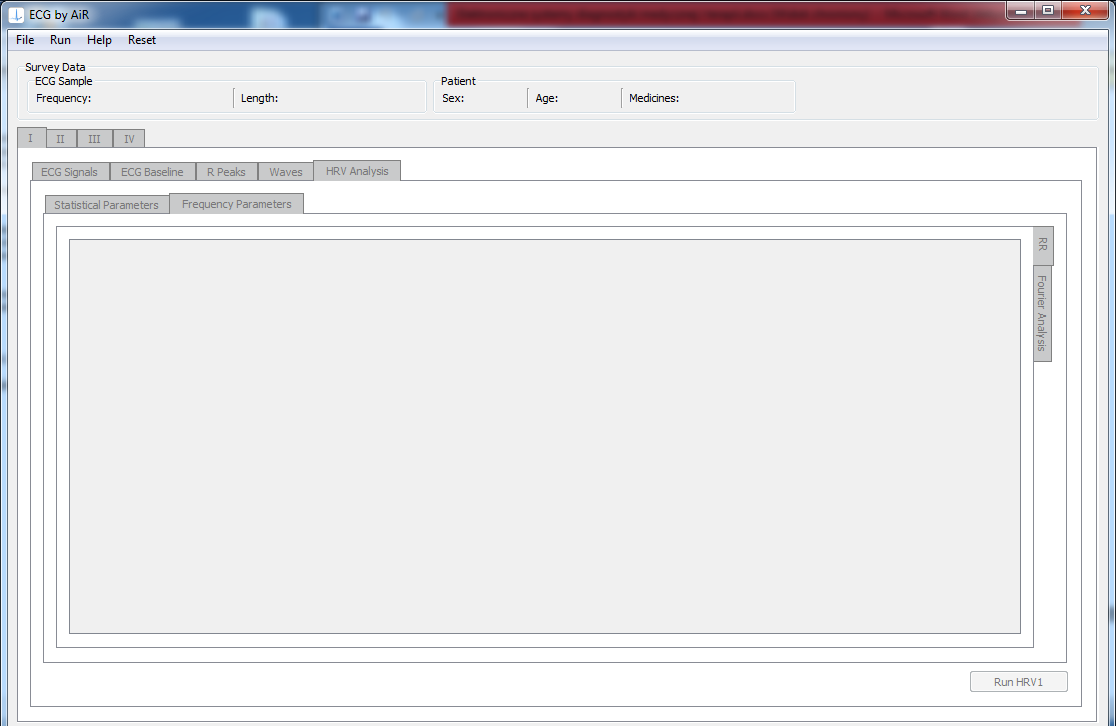
\includegraphics[width=\textwidth]{GUI/img/okno_g}
\label{fig:okno_gi}
\caption{Okno główne programu.}
\end{figure}

Na górze okna głównego znajduje się Menu aplikacji, o następującej strukturze:

\begin{itemize}
\item File
\begin{itemize}
\item Open
\item Exit
\end{itemize}
\item Run
\begin{itemize}
\item Run ECG Baseline
\item Run R Peaks
\item Run Waves
\item HRV Analysis
\item QRS Classification
\item HRT Analysis
\item ST Segment
\item VCG Loop
\item Sig EDR
\item Atrial Fibr
\item QT Disp
\item Sleep apnea
\item RUN ALL
\end{itemize}
\item Help
\begin{itemize}
\item About
\end{itemize}

Opcja File -> Open powoduje uruchomienie okna dialogowego filebrowser, w którym możliwe jest wybranie zestawu danych do przetwarzania.

\begin{figure}[H]
\centering
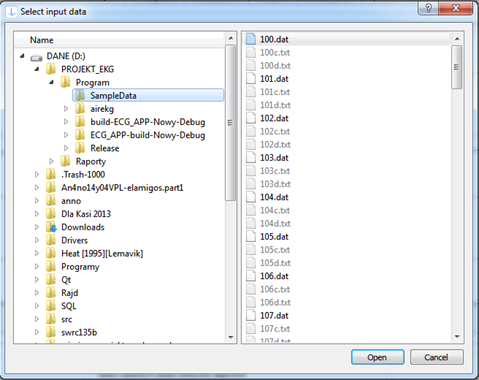
\includegraphics[width=\textwidth]{GUI/img/file_b}
\label{fig:file_b}
\caption{Wybór pliku z danymi.}
\end{figure}

Opcje z grupy Run służą do wywoływania poszczególnych modułów przetwarzających sygnał EKG. Ostatnią z opcji jest RUN ALL wybranie jej powoduje uruchomienie wszystkich modułów EKG w odpowiedniej kolejności. Podczas obliczania odpowiedzi, w dolnej części ekranu pokazywany jest pasek informujący o trwającym przetwarzaniu sygnału.

W grupie Help znajduje się opcja About powoduje ona uruchomienie okna dialogowego, zawierającego informacje o twórcach programu.

Poniżej menu znajdują się pola zawierające dane o sygnale EKG oraz badanym pacjencie: 

\begin{itemize}
\item Częstotliwość pomiaru (Frequency)
\item Długość pomiaru (Length)
\item Płeć (Sex) 
\item Wiek (Age)
\item Przyjmowane leki (Medicines)
\end{itemize}

Po wczytaniu danych, centralną część ekranu zajmuje wykres, przedstawiający sygnał EKG, za pomocą zakładek znajdujących się nad nim  możemy przechodzić do poszczególnych modułów. Moduły zostały podzielone na 4 zakładki w celu ułatwienia poruszania się po programie. W zależności od wybranego modułu, pod wykresem, znajdują się dostępne opcje konfiguracyjne. W każdej zakładce znajduje się przycisk Run pozwalający odpalić konkretny moduł, zaś na dole ekrany do dyspozycji użytkownika jest przycisk RUN ALL uruchamiający wszystkie moduły.
\section{MVC}
\subsection{Moduł wejść}
W projekcie wykorzystane zostały zserializowane dane w formacie binarnym „*.dat”. To oznacza, że program obsługuje tylko pliki z dołączonego do projektu folderu SampleData. W wypadku, kiedy użytkownik chciałby skorzystać z innych danych istnieją dwa rozwiązania:

\begin{itemize}
\item Można wykorzystać skrypt dołączony do projektu (\ref{sec:skrypt}). Aby go uruchomić konieczne jest wcześniejsze pobranie z bazy Physionet oprogramowania ATM.  Ta opcja jest dostępna dla użytkowników,  którzy  chcą pobrać dane zawierające dwa sygnały.
\item Można pobrać oprogramowanie ATM , pobrać odpowiednie pliki i skonwertować je do formatu *.txt . Ta opcja odpowiednia jest dla plików zawierających sygnały z 12 elektrod i wykorzystywana jest tylko w module VCG\_T\_LOOP .
\end{itemize}

Taki sposób wczytywania danych jest optymalny pod względem szybkości działania programu, zdecydowanie utrudnia jednak korzystanie z innego rodzaju danych niż dostarczone. 

\subsection{Struktura aplikacji.}
Istotnym z punktu widzenia rozwoju aplikacji zagadnieniem są współzależności modułów, czyli określenie kolejności wywoływania modułów. Ogólny schemat przedstawiony jest poniżej (\ref{fig:zaleznosci}). Moduły wywoływane są rekurencyjnie w takim sensie, że w przypadku braku potrzebnych danych wywołany zostanie moduł wyżej. W efekcie każdy moduł można uruchomić jednym kliknięciem. W przypadku, w którym odpowiednie dane zostały już przetworzone, wywoływany moduł nie zażąda wywołania modułu nadrzędnego. To oznacza, że po każdej zmianie parametrów wszystkie kolejne moduły należy wywoływać ręcznie, w odpowiedniej kolejności. 

\begin{figure}[H]
\centering
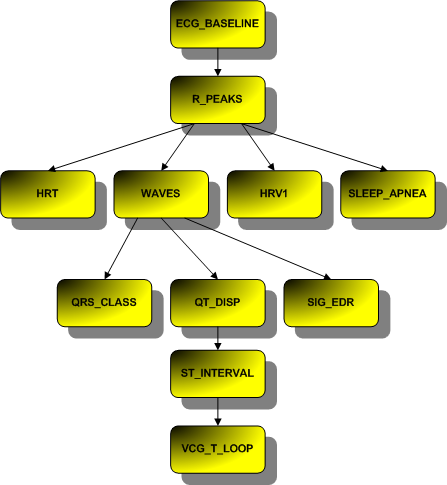
\includegraphics[scale=0.7]{MVC/img/EKG}
\label{fig:zaleznosci}
\caption{Schemat zależności modułow aplikacji}
\end{figure}

Poza modułami w projekcie występują następujące klasy:
\begin{itemize}
\item „appcontroller” czyli klasa zarządzająca całym programem.
\item „airecgmain”, wraz z klasami pomocniczymi, czyli klasa obsługująca GUI.
\item „ecgdata”, wraz z klasami pomocniczymi, czyli klasa przechowująca dane.
\item „ecgentry”, wraz z klasami pomocniczymi, czyli klasa wczytująca dane binarne z pliku.
\end{itemize}

Całość projektu jest tworzona według wzorca Model-View-Controller. Oznacza to, że te trzy części są od siebie wyraźnie rozdzielone. Zarówno widoki (prezentacja wyników), jak i kontroler (interakcja z użytkownikiem) realizowana jest w całości przez GUI. Model (wszystkie obliczenia) wykonywane są w odpowiednich modułach, które nie muszą być dołączane do projektu. Zarządzanie tymi elementami realizowane (czyli silnik aplikacji) realizowane jest przez klasę „appcontroller”. Spełnienie ogólnego wzorca MVC w praktyce oznacza, że klasa appcontroller jest jedyną klasą, która może wymagać modyfikacji po zmodyfikowaniu któregokolwiek innego elementu programu.

\subsection{Logi}

Poza normalnym działaniem aplikacja oferuje również logowanie przebiegu ostatniego wywołania aplikacji z użyciem pakietu QsLog. Do logu zapisywane są najważniejsze zdarzenia i błędy. Raportowany jest także czas wykonania wpisu, co pozwala na oszacowanie szybkości działania poszczególnych modułów, w zależności od wybranych w GUI parametrów. Przykładowy log przedstawiony jest poniżej.

\begin{minipage}{\textwidth}
\begin{verbatim}
 INFO 2014-01-29T22:23:34.965 Program started 
 INFO 2014-01-29T22:24:01.591 Stworzono obiekt typu ecgdata dla pacjenta  "107" . 
 INFO 2014-01-29T22:24:01.756 "649999"  Samples loaded 
 INFO 2014-01-29T22:24:01.841 Reset procedure started: 
 INFO 2014-01-29T22:24:01.841 MVC/ Sleep Apnea deleted 
 INFO 2014-01-29T22:24:01.841 All removed. 
 INFO 2014-01-29T22:24:07.936 Start AtrialFibr 
 INFO 2014-01-29T22:24:07.936 Waves started. 
 INFO 2014-01-29T22:24:07.936 RPeaks stared. 
 INFO 2014-01-29T22:24:07.937 Ecg baseline started. 
 INFO 2014-01-29T22:24:07.937 BASELINE/ Using butterworth filter with coefficiets  "Baseline wander removal (Fs: 360Hz) - [HP, Order: 10, -3db: 0.5Hz]" 
 INFO 2014-01-29T22:24:07.937 MVC/  "V1"  signal will be processed. 
 INFO 2014-01-29T22:24:08.477 Ecg baseline done. 
 INFO 2014-01-29T22:24:08.542 RPeaks/ using Hilbert 
 INFO 2014-01-29T22:24:23.031 RPeaks done. 
 INFO 2014-01-29T22:24:37.838 Waves/ calculated  "2114"  QRS_onset points. 
 INFO 2014-01-29T22:24:37.838 Waves/ calculated  "2114"  QRS_end points. 
 INFO 2014-01-29T22:24:37.838 Waves/ calculated  "1029"  PWaveStart points. 
 INFO 2014-01-29T22:24:37.839 Waves/ calculated  "908"  PWaveEnd points. 
 INFO 2014-01-29T22:24:37.902 GUI/  ecgFrames.Count... "908" 
 INFO 2014-01-29T22:24:37.927 Waves done. 
TRACE 2014-01-29T22:24:37.931 Atrial_FIBR/ calculated parameters: 
 Atrial_FIBR/ PWaveOccurenceRatio:  "0.208941" 
 Atrial_FIBR/ RRIntDivergence:  "0.0319016" 
 Atrial_FIBR/ RRIntEntropy:  "0.219118" 
 INFO 2014-01-29T22:24:37.931 AtrialFibr done 
\end{verbatim}
\end{minipage}

\subsection{Skrypt przetwarzający dane.}
\label{sec:skrypt}

\begin{minipage}{\textwidth}
\begin{verbatim}
REM written by mickl , AGH UST
CLS
@ECHO OFF
ECHO Hello ,
REM ECHO PhysioNet availabl  indexes : 100 -124 , 200-234
REM SET /p index=Please insert record index
SET /a index=100
: loop
IF %index%==125 GOTO assign
IF %index%==235 GOTO quit

ECHO Downloading samples , record #%index%
rdsamp -r mitdb/%index% > %index%a.txt
ECHO Succesfully saved %index%a.txt
ECHO Serializing data
serializer.exe %index%a.txt %index%.dat
DEL %index%a.txt
ECHO Removing 101a.txt
ECHO Downloading annotations, record #%index%
rdann -r mitdb/%index% -a atr > %index%c.txt
ECHO Succesfully saved %index%c.txt
ECHO Downloading notes , record #%index%
wfdbdesc mitdb/%index% >%index%d.txt
ECHO Succesfully saved %index%d.txt

SET /a index=%index%+1
GOTO loop

: assign
SET /a index=200
GOTO loop

: quit
ECHO All records converted
\end{verbatim}
\end{minipage}
\section{Moduł ECG\_BASELINE}

\subsection{Wstęp}

Zagadnienie usuwania zakłóceń z sygnału EKG jest szeroko omawiane w literaturze. Wynika to z popularności badania, a także wyzwania stawianego inżynierom -- sygnał ten ma niewielką amplitudę, a zakłócenia pochodzą z wielu źródeł -- głównie mięśni, elektrod, linii zasilającej urządzenia badawczego i rytmu oddechowego pacjenta \cite{Sayadi2008}.  Kolejnym utrudnieniem jest fakt, że ich pasmo zakłóceń zazwyczaj pokrywa się z sygnałem użytecznym -- zachodzi więc obawa, że wstępne filtrowanie sygnału może zniekształcić jego interesującą część \cite{Jane1992}. 

W ciągu ostatnich dekad wielu naukowców pracowało nad opracowaniem metod usuwania szumu z sygnału EKG. Manpreet Kaur \cite{Kaur2011} w swym przeglądzie porównuje filtry IIR, FIR, średnią kroczącą, metodę splajnów oraz oparty o transformację falkową. Ten ostatni dekomponuje sygnał w bazie db4, a następnie usuwa tę część sygnału, która jest najwolniej zmienna. Filtrem najlepiej odszumiającym sygnał okazał się IIR o zerowym przesunięciu fazowym. Jego wyjście cechowało się najwyższym SNR oraz brakiem modyfikacji sygnału użytecznego. Na chwilę obecną prawdziwe wyzwanie stanowi jednak filtrowanie EKG płodu. Jego odczyt przy szumie pochodzącym od EKG matki jest wyjątkowo trudny \cite{Prasanth2013}. Nastała potrzeba opracowania skuteczniejszych metod filtracji sygnału.

W ostatnich latach popularność zyskała metoda filtracji sygnału w oparciu o adaptacyjny filtr Kalmana, ze względu na jego zdolność do jednoczesnego modelowania zarówno sygnału EKG, jak i izolinii \cite{Sayadi2008,Mneimneh2006}.  Naukowcy z Marquette University w swym artykule \cite{Mneimneh2006} wykazali wyższą skuteczność w usunięciu izolinii dla filtru Kalmana, zbudowanego w oparciu o model autoregresyjny, w porównaniu do średniej kroczącej i metody splajnów rzędu trzeciego. Charakteryzował się on nie tylko mniejszą średnią wariancją błędu, lecz także mniejszym zniekształceniem sygnału użytecznego w porównaniu do pozostałych. Niestety, zastosowane podejście okazało się nieskuteczne w przypadku szybkich zmian poziomu izolinii. Przyjęcie liniowego modelu EKG wydaje się zbytnim uproszczeniem.

Alternatywne podejście, wykorzystujące rozszerzony filtr Kalmana, zostało zaprezentowane w \cite{Sameni2005-1, Sameni2005-2}. Jego genezę stanowiły prace nad stworzeniem generatora EKG, opartego na nielinowym modelu matematycznym, uwzględniającym morfologię kompleksu QPRST i kształtu fali R-R. Jego prostota i elastyczność umożliwiają dobrą estymację sygnału EKG, również w przypadku jego chwilowego zaniku. W ramach swych prac autorzy udostępnili również narzędzie do automatycznej optymalizacji parametrów modelu. Naszym zdaniem wykorzystanie rozszerzonego filtru Kalmana, w oparciu o wyżej wspomniany model, to najbardziej obiecujący sposób na usunięcie szumu z zapisu EKG. Z uwagi na pracę off-line, kwestie złożoności obliczeniowej takiego rozwiązania są mniej ważne od jego ostatecznej skuteczności. 

W module ECG\_BASELINE zaimplementowane zostały następujące metody filtracji sygnału EKG: 
\begin{itemize}
\item Filtr Butterwortha (do usunięcia falowania izolinii oraz szumu sieci elektrycznej 50 Hz)
\item Średnia krocząca
\item Filtr Savitzky'ego-Golay'a
\item Rozszerzony filtr Kalmana
\end{itemize}

\subsection{Proponowane rozwiązanie}

W sekcji tej opisane zostały zaimplementowane filtry, z pominięciem filtru Savitzky'ego-Golay'a, ze względu na brak zmian w jego obrębie w stosunku do poprzedniej wersji modułu ECG\_BASELINE, opisanej w pracy~\cite{Baseline2013}.

\subsubsection{Filtr Butterwortha}

Filtr Butterwortha jest filtrem cyfrowym o nieskończonej odpowiedzi impulsowej (IIR -- \emph{Infinite Impulse Response}. Jest on odpowiednikiem filtru analogowego i ma realizowalną fizycznie transmitancję. W dowolnej chwili, wyjście filtru zależy od $N$ próbek wejściowych i $N$ poprzednich próbek wyjściowych, gdzie $N$ oznacza rząd filtru. Taka budowa prowadzi do problemów w implementacji -- ze względu na niezerowy błąd wynikający ze skończonej długości reprezentacji liczby zmiennoprzecinkowej, filtr IIR wysokiego rzędu będzie niestabilny numerycznie. W celu osiągnięcia odpowiedniej charakterystyki filtru, przy jednoczesnym uniknięciu problemów ze stabilnością numeryczną, filtry o nieskończonej odpowiedzi impulsowej implementuje się jako kaskadowo połączone sekcje filtrów drugiego rzędu. Transmitancja takiej sekcji wyraża się równaniem

\begin{equation}
H(z) = \frac{b_0 + b_1z^{-1} + b_2z^{-2}}{1 + a_1z^{-1} + a_2z^{-2}}
\end{equation}

Bezpośrednie wykorzystanie filtru Butterwortha napotykać może problemy wynikające z silnego, nieliniowego zniekształcenia fazy w okolicy częstotliwości odcięcia. Kolejnym problemem jest duże zniekształcenie sygnału w pierwszych sekundach przetwarzanego sygnału (\emph{transient}), mogące utrudnić działanie algorytmów automatycznej analizy sygnałów EKG. W celu rozwiązania tych problemów, stosuje się nieprzyczynowy filtr o zerowym przesunięciu fazowym, o strukturze przedstawionej na rysunku~\ref{fig:0phase} oraz rozszerza się sygnał o część przebiegu odbitą względem $OX$. Liczbę odbitych próbek oblicza się ze wzoru

\begin{equation}
t_r = \ceil{\min_k\frac{\pi}{\abs{p_k} \cdot \varphi(p_k)}}
\end{equation}

gdzie $p_k$ to bieguny transmitancji filtru, zaś $\varphi(p_k)$ określa argument zmiennej zespolonej $p_k$.

\begin{figure}[H]
\centering
	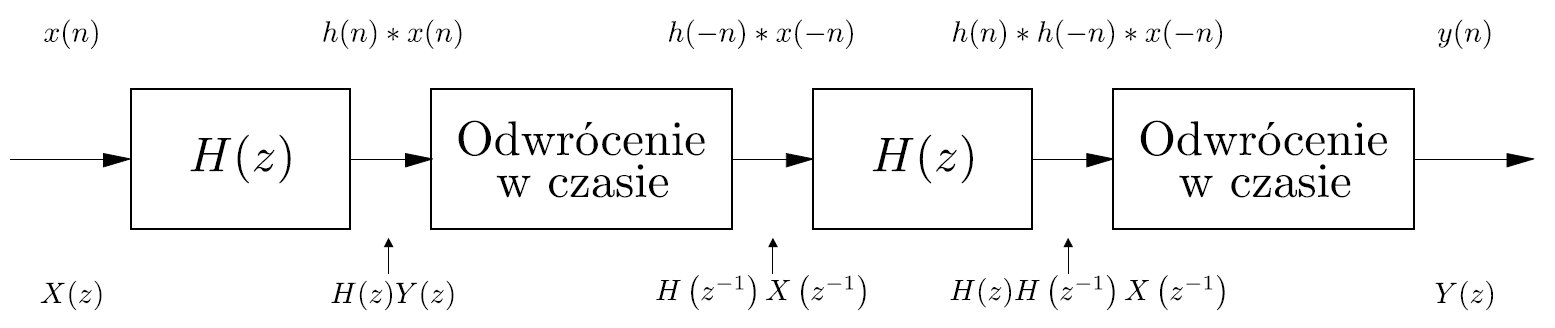
\includegraphics[width=\textwidth]{ECG_BASELINE/figures/butter_0phase.png}
\caption{Struktura nieprzyczynowego filtru o zerowym przesunięciu fazowym. Źródło: \cite{Baseline2013}}
\label{fig:0phase}
\end{figure}

Kolejnym problemem, na jaki natrafić można przy implementacji filtrów IIR jest ich niestabilność. Wszystkie filtry o skończonej odpowiedzi impulsowej (FIR -- \emph{Finite Impulse Response}) są z natury stabilne, ze względu na postać ich transmitancji -- brak w nich sprzężenia zwrotnego, przez co wszystkie ich bieguny znajdują się w początku układu współrzędnych. Filtry IIR posiadają sprzężenie zwrotne, przez co mogą być niestabilne -- w trakcie ich projektowania należy zadbać, aby wszystkie bieguny znajdowały się w obrębie okręgu jednostkowego na płaszczyźnie zespolonej $\mathbb{C}$. Wszystkie filtry opisane w tej pracy spełniają ten warunek.

Dla filtru Butterwortha dostępne w aplikacji są następujące zestawy współczynników:

\begin{itemize}

\item Usunięcie falowania izolinii
\begin{itemize}
\item Rząd filtru: 10 (rząd efektywny: 20)
\item Filtr wysokoprzepustowy, punkt -3db ustawiony na 0.5 Hz
\item Częstotliwości próbkowania: 250/360 Hz
\end{itemize}

\item Usunięcie szumu sieci elektrycznej 50 Hz
\begin{itemize}
\item Rząd filtru: 10 (rząd efektywny: 20)
\item Film pasmowozaporowy, punkty -3db ustawione na 49.5 Hz i 50.5 Hz
\item Częstotliwości próbkowania 250/360 Hz
\end{itemize}

\item Usunięcie 3 składowej harmonicznej szumu sieciowego o częstotliwości 150 Hz
\begin{itemize}
\item Rząd filtru: 10 (rząd efektywny: 20)
\item Filtr pasmowozaporowy, punkty -3db ustawione na 149.5 Hz i 150.5 Hz
\item Częstotliwość próbkowania: 360 Hz
\end{itemize}

\end{itemize}

Współczynniki oraz charakterystyki poszczególnych filtrów zostaną teraz przedstawione dla pojedynczej częstotliwości próbkowania.

\subsubsection{Filtr usuwający falowanie izolinii}

Współczynniki filtru dla częstotliwości próbkowania $f_s=250 Hz$ zebrane zostały w tabeli~\ref{tab:bw_250}. Charakterystyka amplitudowa i charakterystyka fazowa przedstawione zostały na rysunku~\ref{fig:bw_250}.

\begin{table}[H]
\begin{center}
\begin{tabular}{|c|c|c|c|c|}
\hline
        $b_0$ & $b_1$ & $b_2$ & $a_1$ & $a_2$ \\
\hline
        1& -2& 1& -1.99591858803741& 0.996076189822218\\
\hline
        1& -2& 1& -1.98849798039776& 0.988654996236322\\
\hline
        1& -2& 1& -1.98222892979253& 0.982385450614125\\
\hline
        1& -2& 1& -1.97769893355394& 0.977855096677832\\
\hline
        1& -2& 1& -1.97532566755629& 0.975481643282286\\
\hline
\end{tabular}
\caption{Współczynniki filtru Butterwortha do usuwania falowania izolinii dla $f_s=250 Hz$}
\label{tab:bw_250}
\end{center} 
\end{table}

\begin{figure}[H]
\centering
	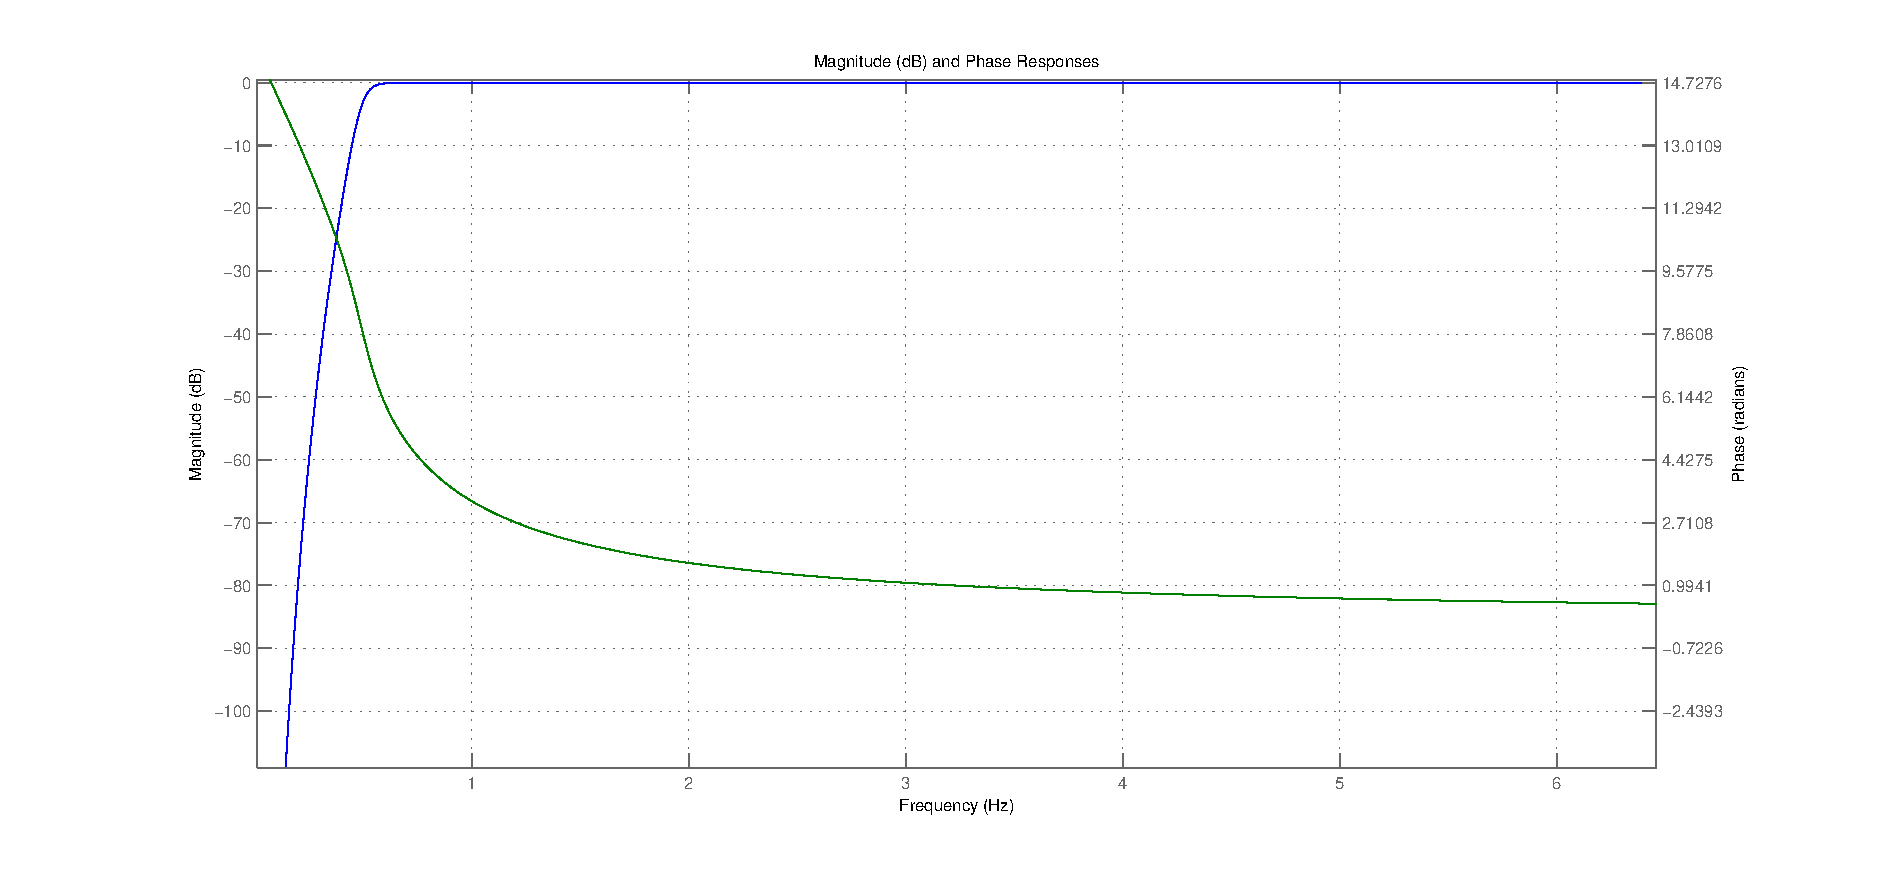
\includegraphics[width=\textwidth]{ECG_BASELINE/figures/bw_250.eps}
\caption{Charakterystyka amplitudowo i charakterystyka fazowa filtru Butterwortha do usuwania falowania izolinii dla $f_s=250 Hz$}
\label{fig:bw_250}
\end{figure}


\subsubsection{Filtr usuwający szum sieci elektrycznej 50 Hz oraz jego 3. harmoniczną}

Współczynniki filtru usuwającego szum sieciowy 50 Hz z sygnału próbkowanego z $f_s = 360$  zebrane zostały w tabeli~\ref{tab:ac_360}. Charakterystyka amplitudowa i charakterystyka fazowa przedstawione zostały na rysunku~\ref{fig:50hz_360}.

\begin{table}[H]
\begin{center}
\begin{tabular}{|c|c|c|c|c|}
\hline
        $b_0$ & $b_1$ & $b_2$ & $a_1$ & $a_2$ \\
\hline
        1& -1.28562417200218& 1& -1.26937327532045&        0.994584016960900\\
\hline
        1& -1.28562417200218& 1& -1.29478401747452&        0.994658733271036\\
\hline
        1& -1.28562417200218& 1& -1.26873553509657&        0.985919061981878\\
\hline
        1& -1.28562417200218& 1& -1.28442034996815&        0.986038923952812\\
\hline
        1& -1.28562417200218& 1& -1.27450176361204&        0.982697263115690\\
\hline
\end{tabular} 
\caption{Współczynniki filtru Butterwortha do usuwania szumu sieciowego 50 Hz dla $f_s=360 Hz$}
\label{tab:ac_360}
\end{center}
\end{table}

\begin{figure}[H]
\centering
	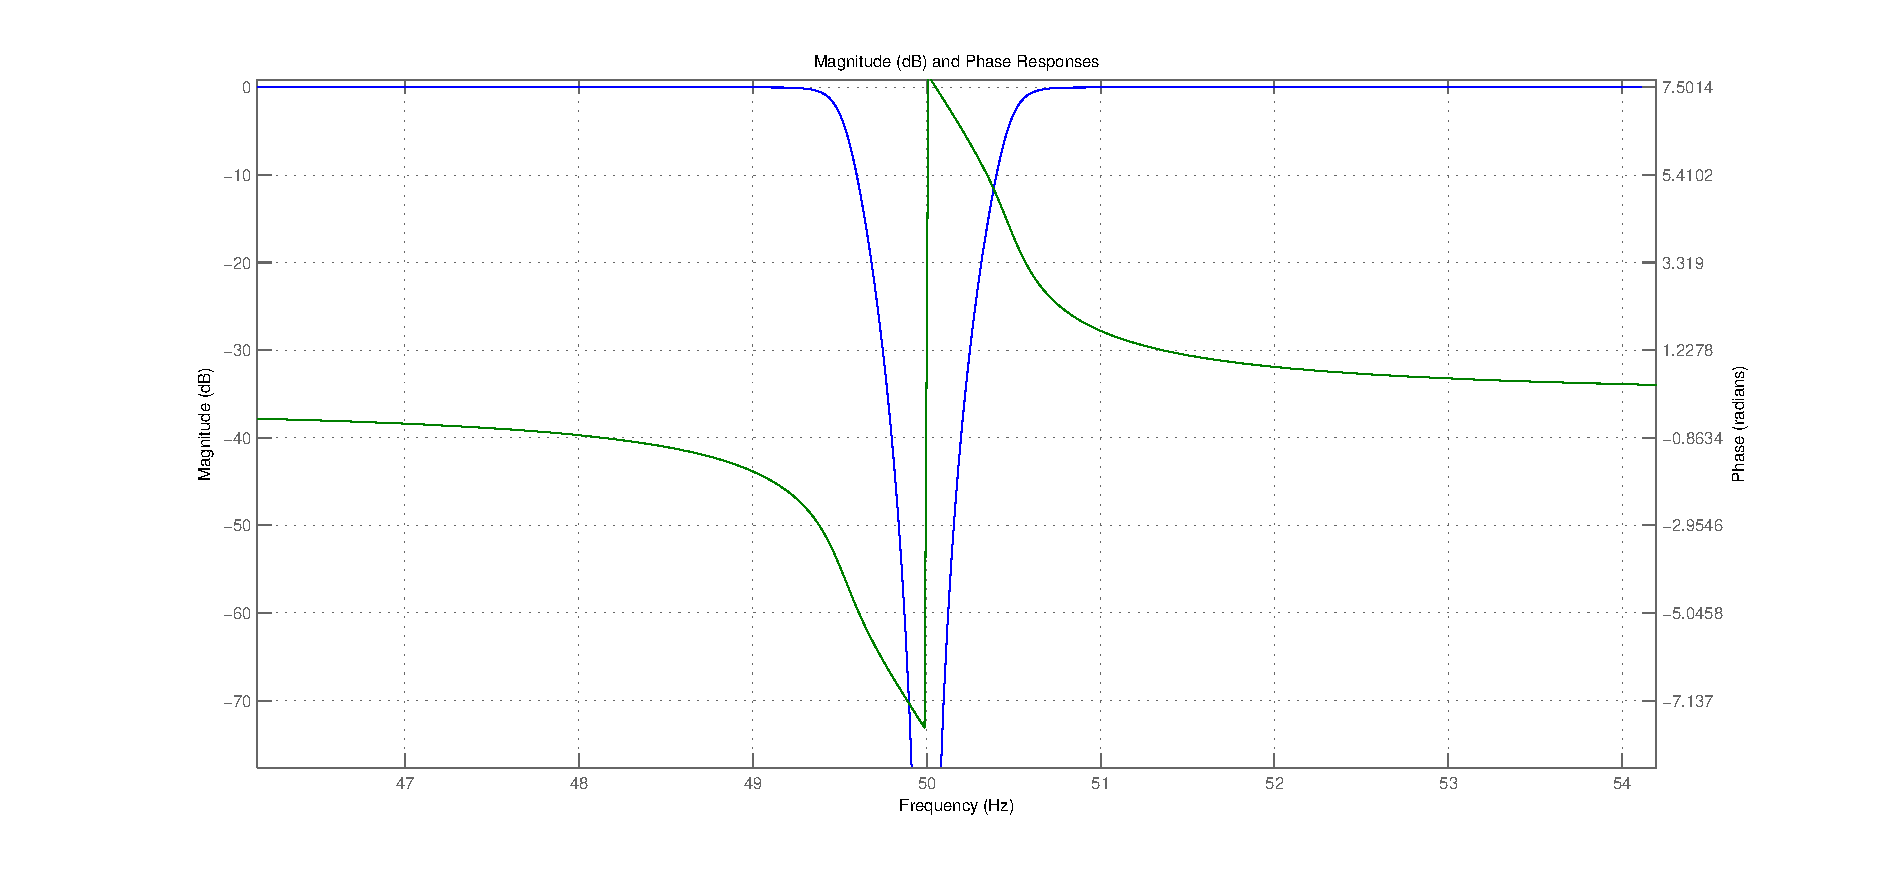
\includegraphics[width=\textwidth]{ECG_BASELINE/figures/50hz_360.eps}
\caption{Charakterystyka amplitudowa i fazowa filtru Butterwortha do usuwania szumu sieciowego 50 Hz dla $f_s=360 Hz$}
\label{fig:50hz_360}
\end{figure}

\newpage{}

Współczynniki filtru usuwającego 3. harmoniczną szumu sieciowego 50 Hz dla częstotliwości próbkowania sygnału $f_s = 360 Hz$ zebrane są w tabeli~\ref{tab:ac_3rd_360}. Charakterystyka amplitudowa i charakterystyka fazowa przedstawione zostały na rysunku~\ref{fig:3rd_360}.

\begin{table}[H]
\begin{center}
\begin{tabular}{|c|c|c|c|c|}
\hline
        $b_0$ & $b_1$ & $b_2$ & $a_1$ & $a_2$ \\
\hline
        1& 1.73211676126764& 1&        1.71899593699765& 0.994544262243386\\
\hline
        1& 1.73211676126764& 1&        1.73568383808774& 0.994698492564272\\
\hline
        1& 1.73211676126764& 1&        1.71472803758620& 0.985855276540036\\
\hline
        1& 1.73211676126764& 1&        1.72512958096071& 0.986102721276756\\
\hline
        1& 1.73211676126764& 1&        1.71713158098109& 0.982697263115690\\
\hline
\end{tabular} 
\caption{Współczynniki filtru Butterwortha do usuwania 3. harmonicznej szumu sieciowego 50 Hz dla $f_s=360 Hz$}
\label{tab:ac_3rd_360}
\end{center}
\end{table}

\begin{figure}[H]
\centering
	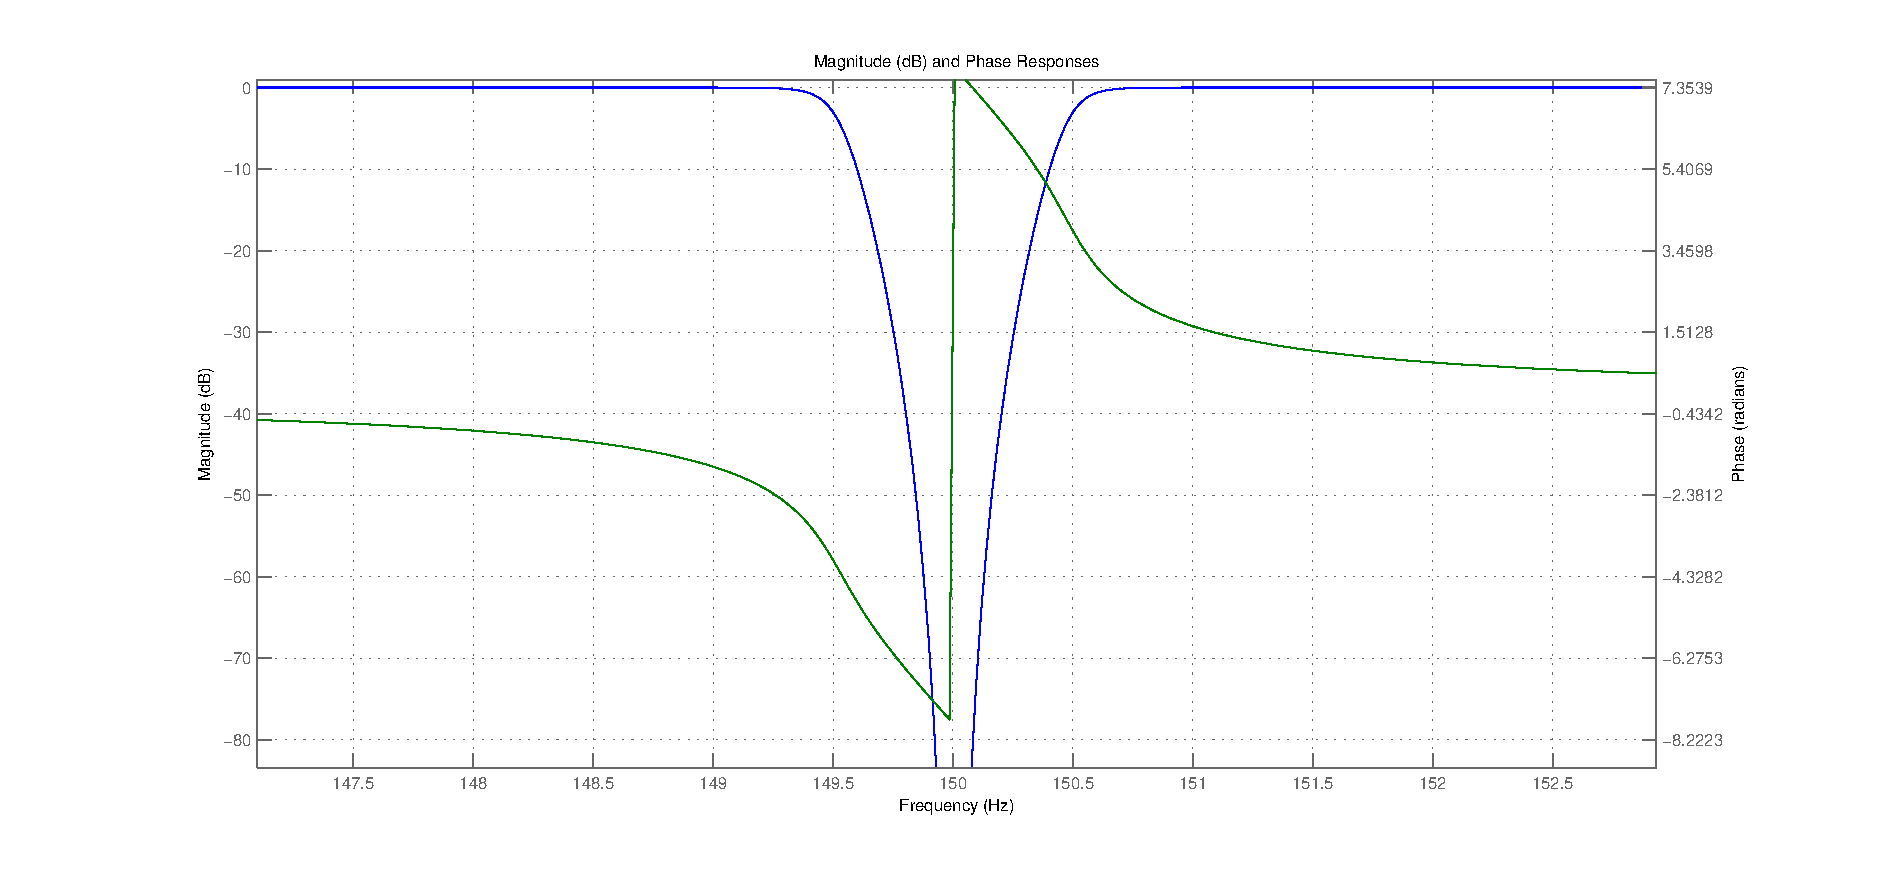
\includegraphics[width=\textwidth]{ECG_BASELINE/figures/3rd_harm_360.eps}
\caption{Charakterystyka amplitudowa i fazowa filtru Butterwortha do usuwania 3. harmonicznej szumu sieciowego 50 Hz dla $f_s=360 Hz$}
\label{fig:3rd_360}
\end{figure}

\subsubsection{Średnia krocząca}

Średnia krocząca (MA -- \emph{Moving Average}) jest jednym z najprostszych filtrów cyfrowych. Równanie średniej kroczącej jest następujące

\begin{equation}
y[i] = \frac{1}{M}\sum_{j=0}^{M-1}x[i - j]
\end{equation}

gdzie $y$ jest sygnałem wyjściowym, $x$ -- sygnałem wejściowym, zaś $M$ to ilość próbek wchodzących w skład średniej. 

Średnia krocząca jest filtrem o działaniu uśredniającym, o właściwościach dolnoprzepustowego filtru o skończonej odpowiedzi impulsowej. W celu zastosowania tego filtru do usunięcia falowania izolinii, konieczne jest odjęcie otrzymanego wyjścia filtru od każdej próbki sygnału wejściowego, zgodnie z równaniem

\begin{equation}
y_{hp}[i] = x[i] - y[i]
\end{equation}

Implementacja średniej kroczącej zawarta w module ECG\_BASELINE zmodyfikowana została w sposób umożliwiający jej wywołanie z podaniem czasu uśredniania $t_a$ oraz częstotliwości próbkowania sygnału $f_s$. Ilość próbek wchodzących w skład średniej $M$ jest wtedy wyliczana z wzoru

\begin{equation}
M = \ceil{t_a \cdot f_s}
\end{equation}


\subsubsection{Rozszerzony Filtr Kalmana}
Konstrukcja filtru Kalmana powstała w oparciu o \cite{Sameni2005-1, Sameni2005-2} i przedstawiona w formie algorytmicznej. Podstawy teoretyczne metody oraz szczegóły poszczególnych kroków algorytmu znajdują się w dalszej części rozdziału.

Algorytm odszumiania zapisu EKG przy użyciu rozszerzonego filtru Kalmana
\begin{enumerate}
\item Usuń izolinię sygnału EKG (np. przy użyciu średniej kroczącej)
\item Zidentyfikuj parametry modelu nieliniowego
\item Dopasuj model do średniego przebiegu wejściowego sygnału
\item Przeprowadź filtrację sygnału, wykorzystując rozszerzony, wygładzający filtr Kalmana
\end{enumerate}

Dyskretny Filtr Kalmana estymuje stan dyskretnego systemu dynamicznego, opisanego liniowym, stochastycznym równaniem różnicowym:
\begin{equation}
 x_k = Ax_{k-1} + Bu_{k-1} + w_{k-1}
\end{equation}
z wyjściem opisanym równaniem:
\begin{equation}
 z_k = Hx_k + \upsilon_k
\end{equation}

Zmienne losowe $w_k, \upsilon_k$ reprezentują odpowiednio szum procesu i pomiaru. Zakładamy, że są one niezależne od siebie i charakteryzują się rozkładem normalnym:
\begin{equation}
\begin{split}
 p(w) \sim N(0,Q) \\
 p(\upsilon) \sim N(0,R)
 \end{split}
\end{equation}

\begin{figure}
\centering
	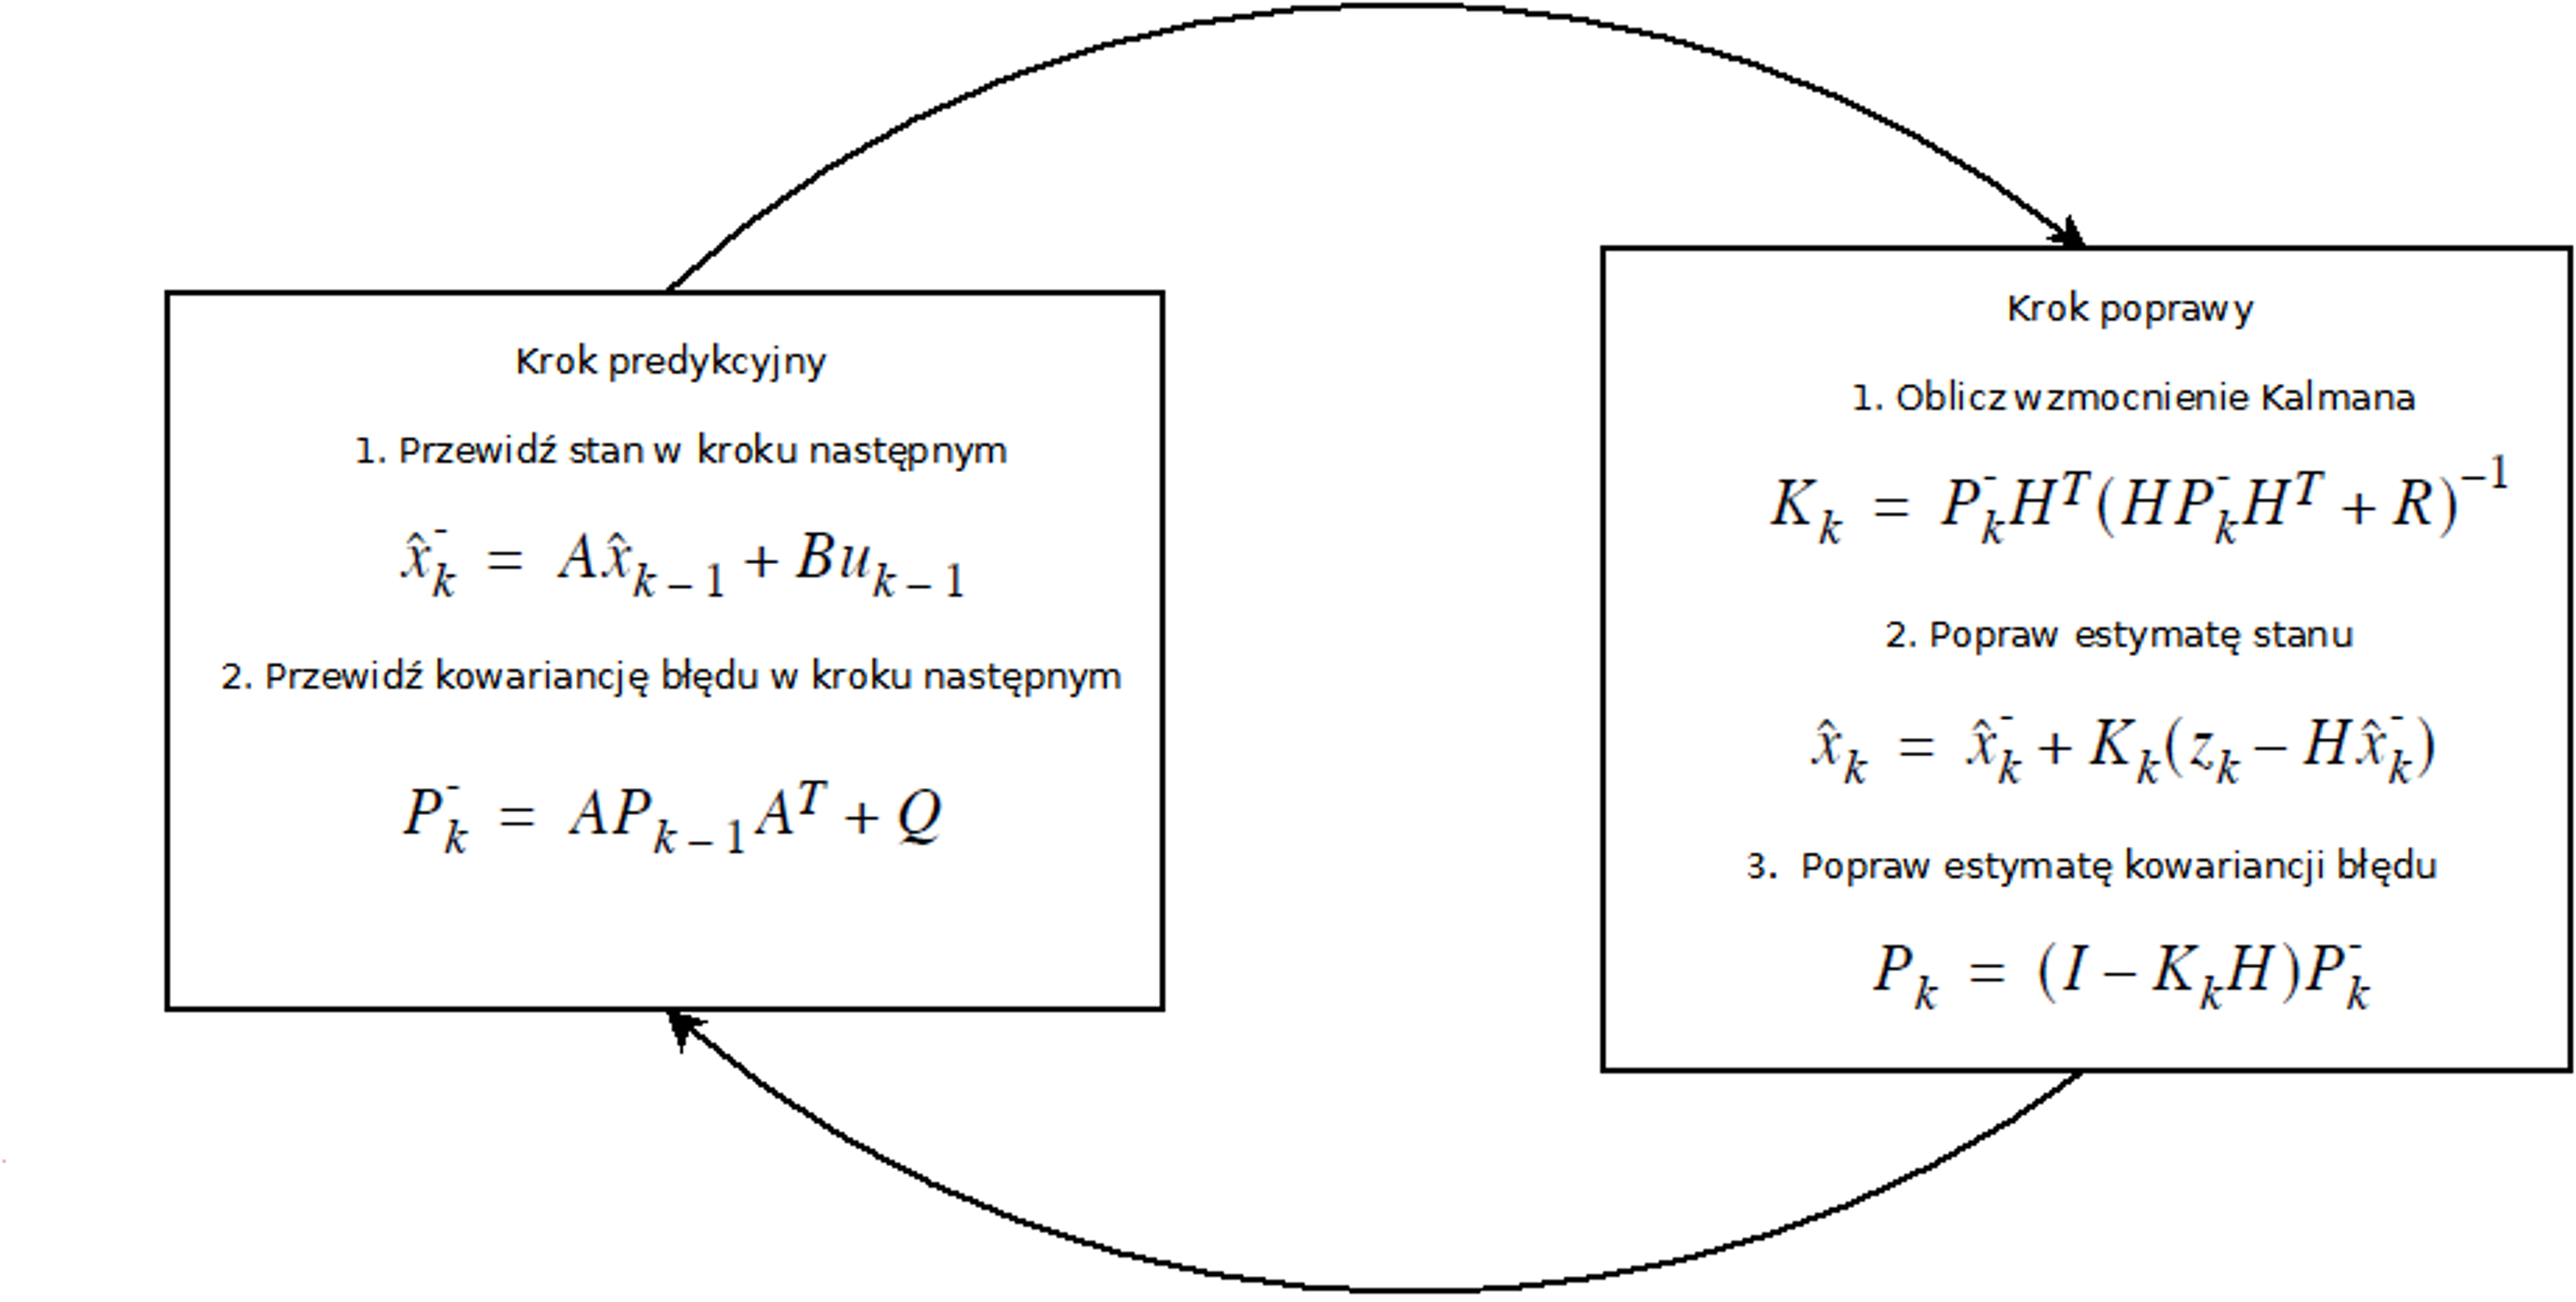
\includegraphics[width=\textwidth]{ECG_BASELINE/figures/KF.png}
\caption{Działanie filtru Kalmana}
\label{Kalman}
\end{figure}

Rysunek \ref{Kalman} przedstawia schemat ideowy dyskretnego filtru Kalmana. W pierwszym kroku („predykcyjnym”) estymowany jest obecny stan modelu na podstawie stanu poprzedniego. Następnie, krok „korekcyjny” służy uwzględnieniu obecnych pomiarów i naniesieniu poprawki na stan. Wpływ stanu poprzedniego i obecnego pomiaru na stan obecny jest determinowany przez macierze $R$ i $Q$, wyznaczane w procesie identyfikacyjnym. Występująca w równaniach macierz $P$ oznacza kowariancję estymaty błędu modelu. Rozszerzony filtr Kalmana, w przeciwieństwie do swej klasycznej wersji, estymuje stan nieliniowego systemu dynamicznego, linearyzując go w otoczeniu stanu poprzedniego, zakładając, że chwilowe wartości $w_k, \upsilon_k$ wynoszą 0. 
Wygładzający filtr Kalmana dokonuje estymacji stanu, wykorzystując wszystkie pomiary sygnału, pobrane w stałych odstępach czasu. Wykorzystano tu fakt, że filtracji sygnału dokonujemy off-line, a zatem wszystkie pomiary zostały już zgromadzone. W tym celu najczęściej wykorzystuje się algorytm Rachua-Tunga-Striebela, który dzieli się na dwa etapy. W pierwszym kroku uruchamia się zwyczajny filtr Kalmana i zachowuje się estymaty stanu $x_{k|k}$ i kowariancje $P_{k|k}$ do użycia w kroku drugim. Następny etap polega na obliczeniu wygładzonych estymat stanu $x_{k|n}$ i kowariancji $P_{k|n}$, zaczynając od końca sygnału, z wykorzystaniem następujących, rekurencyjnych równań:
\begin{equation}
\begin{cases}
	\hat{x}_{k|n} &= \hat{x}_{k|k} + C_k(\hat{x}_{k+1|n} - \hat{x}_{k+1|k}) \\
	P_{k|n} &= P_{k|k} + C_k(P_{k+1|n} - P_{k+1|k})C_{k}^T
\end{cases}
\end{equation}
Gdzie:
\begin{equation}
\begin{split}
	C_k = P_{k|k} \cdot A_{k}^T \cdot P_{k+1|k} ^{-1}
\end{split}
\end{equation}

\subsubsection{Model matematyczny}
W oparciu o \cite{Sameni2005-1}, przyjęty następujący, dyskretny model matematyczny, opisany we współrzędnych biegunowych:
\begin{equation}
\begin{cases}
	\theta[k+1] &= \theta[k] + \omega \Delta \\
	z[k+1] &= \sum_{i \in {P, Q, R, S, T} } \Delta a_i \Delta \theta_i \exp \left({- \frac{\Delta \theta_i^2}{2 b_i^2}} \right) + z[k] + N \Delta
\end{cases}
\label{eq:model1}
\end{equation}

Zmiennymi stanu modelu są: $\theta$ -- faza sygnału i $z$ -- jego amplituda. Ponadto, $\Delta$ to czas próbkowania, a $\Delta \theta_i = (\theta - \theta_i)mod(2 \pi)$. $N$ to addytywny szum, modelujący izolinię oraz inne zakłócenia procesowe. Rzut powyższego modelu na oś $z$ przedstawia sygnał EKG.

W celu wykorzystania powyższego modelu w implementacji rozszerzonego filtru Kalmana, należy również uzyskać jego zlinearyzowaną postać. Przyjmując:
\begin{equation}
\begin{cases}
	\theta[k+1] &= F(\theta, z, \omega, k) \\
	z[k+1] &=  G(\theta, z, a_i, \theta_i, b_i, N, k)
\end{cases}
\label{eq:model-lin1}
\end{equation}

następujące równania przedstawiają zlinearyzowany model ze względu na zmienne stanu $\theta$ i $z$. 

\begin{equation}
\begin{split}
	\frac{\partial F}{\partial z} &= 0 \\
	\frac{\partial F}{\partial \theta} &= \frac{\partial G}{\partial z} = 1 \\
	\frac{\partial G}{\partial \theta} &= \sum_{i \in {P, Q, R, S, T} } - \Delta a_i \left( 1 - \frac{\Delta \theta_i^2}{b_i^2} \right) \exp \left({- \frac{\Delta \theta_i^2}{2 b_i^2}} \right)
\end{split}
\label{eq:model-lin2}
\end{equation}

Podobnie, układ równań~\ref{eq:model-lin3} to wynik linearyzacji równania~\ref{eq:model-lin1} w zależności od szumów procesowych.

\begin{equation}
\begin{split}
	\frac{\partial F}{\partial a_i} &= \frac{\partial F}{\partial b_i} = \frac{\partial F}{\partial \theta_i} = \frac{\partial F}{\partial N} = 0 \\
	\frac{\partial F}{\partial \omega} &= \Delta \\
	\frac{\partial G}{\partial a_i} &= - \Delta \cdot \Delta \theta_i \exp \left({- \frac{\Delta \theta_i^2}{2 b_i^2}} \right), i \in {P, Q, R, S, T} \\
	\frac{\partial G}{\partial b_i} &= - \Delta a_i \frac{\Delta \theta_i^3}{b_i^3} \exp \left({- \frac{\Delta \theta_i^2}{2 b_i^2}} \right) \\
	\frac{\partial G}{\partial \omega} &= 0 \\
	\frac{\partial G}{\partial \theta_i} &= \Delta a_i \left[1 - \frac{\Delta \theta_i^2}{b_i^2} \right] \exp \left({- \frac{\Delta \theta_i^2}{2 b_i^2}} \right) \\
	\frac{\partial G}{\partial N} &= \Delta 
\end{split}
\label{eq:model-lin3}
\end{equation}

Szum procesowy może być oznaczony jako $\underline{w}_k = \left[ a_P,...,a_T,b_P,...,b_T, \theta_P,...,\theta_T,\omega,N \right]$, a $Q_k = E \{\underline{w}_k, \underline{w}_k^T \}$. Tym samym model dynamiczny jest przygotowany do wykorzystania w rozszerzonym filtrze Kalmana.

\subsection{Testy filtrów}

\subsubsection{Filtr Butterwortha}

Wyniki części przeprowadzonych testów nowych zestawów współczynników dla fitru Butterwortha przedstawiono na rysunkach~\ref{fig:bw_removal_comparison},~\ref{fig:bw_removal_zoom},~\ref{fig:50hz_comparison},~\ref{fig:50hz_zoom}.

\begin{figure}[H]
\centering
	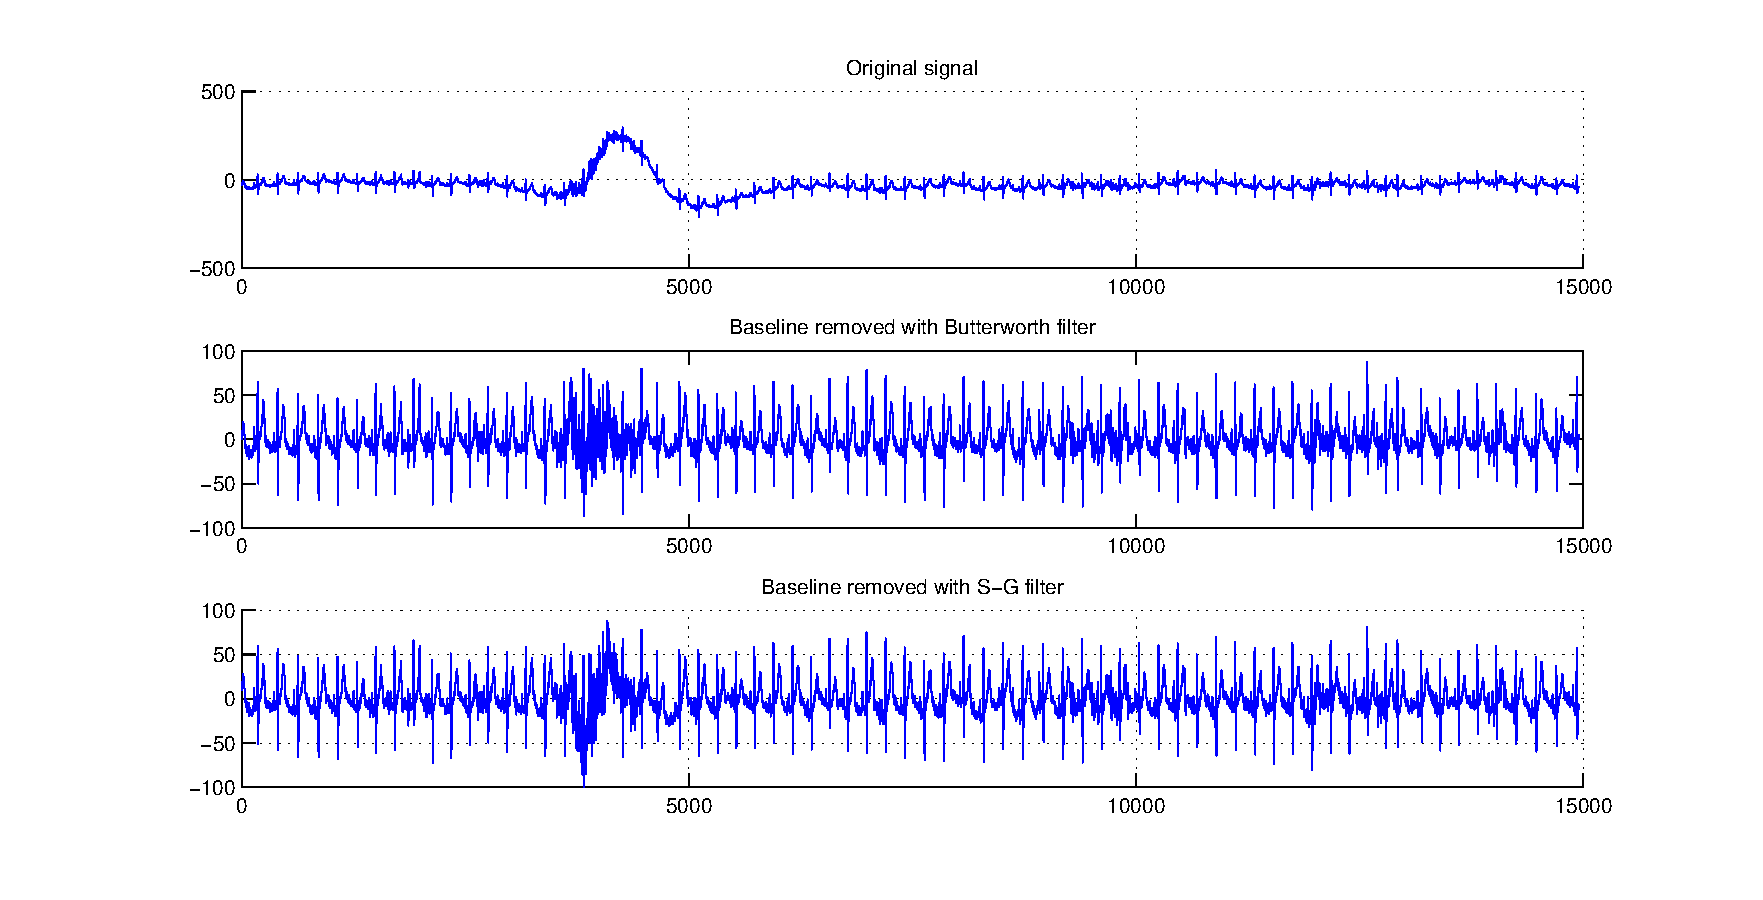
\includegraphics[width=\textwidth]{ECG_BASELINE/figures/250_baseline_comparison.eps}
\caption{Porównanie działania filtru Butterwortha i filtru Savitzky'ego-Golay'a do usuwania falowania izolinii z sygnału próbkowanego z częstotliwością $f_s=250 Hz$}
\label{fig:bw_removal_comparison}
\end{figure}

\begin{figure}[H]
\centering
	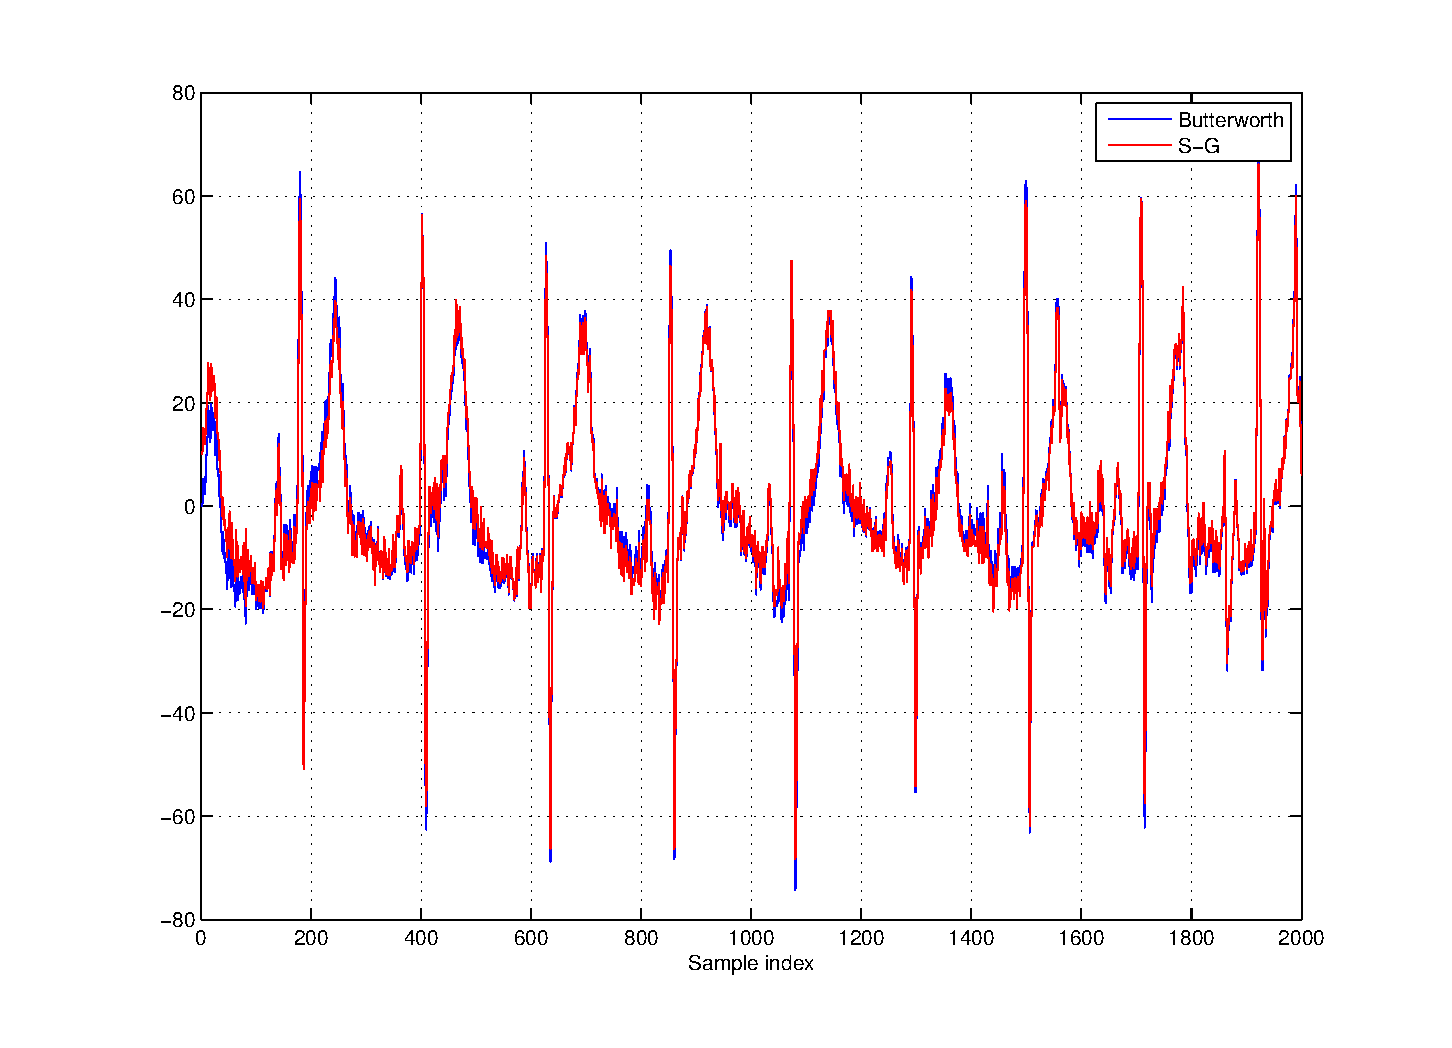
\includegraphics[width=0.7\textwidth]{ECG_BASELINE/figures/zoom_butter_sg.eps}
\caption{Powiększony fragment przebiegów wyjścia filtru S-G i Butterwortha.}
\label{fig:bw_removal_zoom}
\end{figure}

\begin{figure}[H]
\centering
	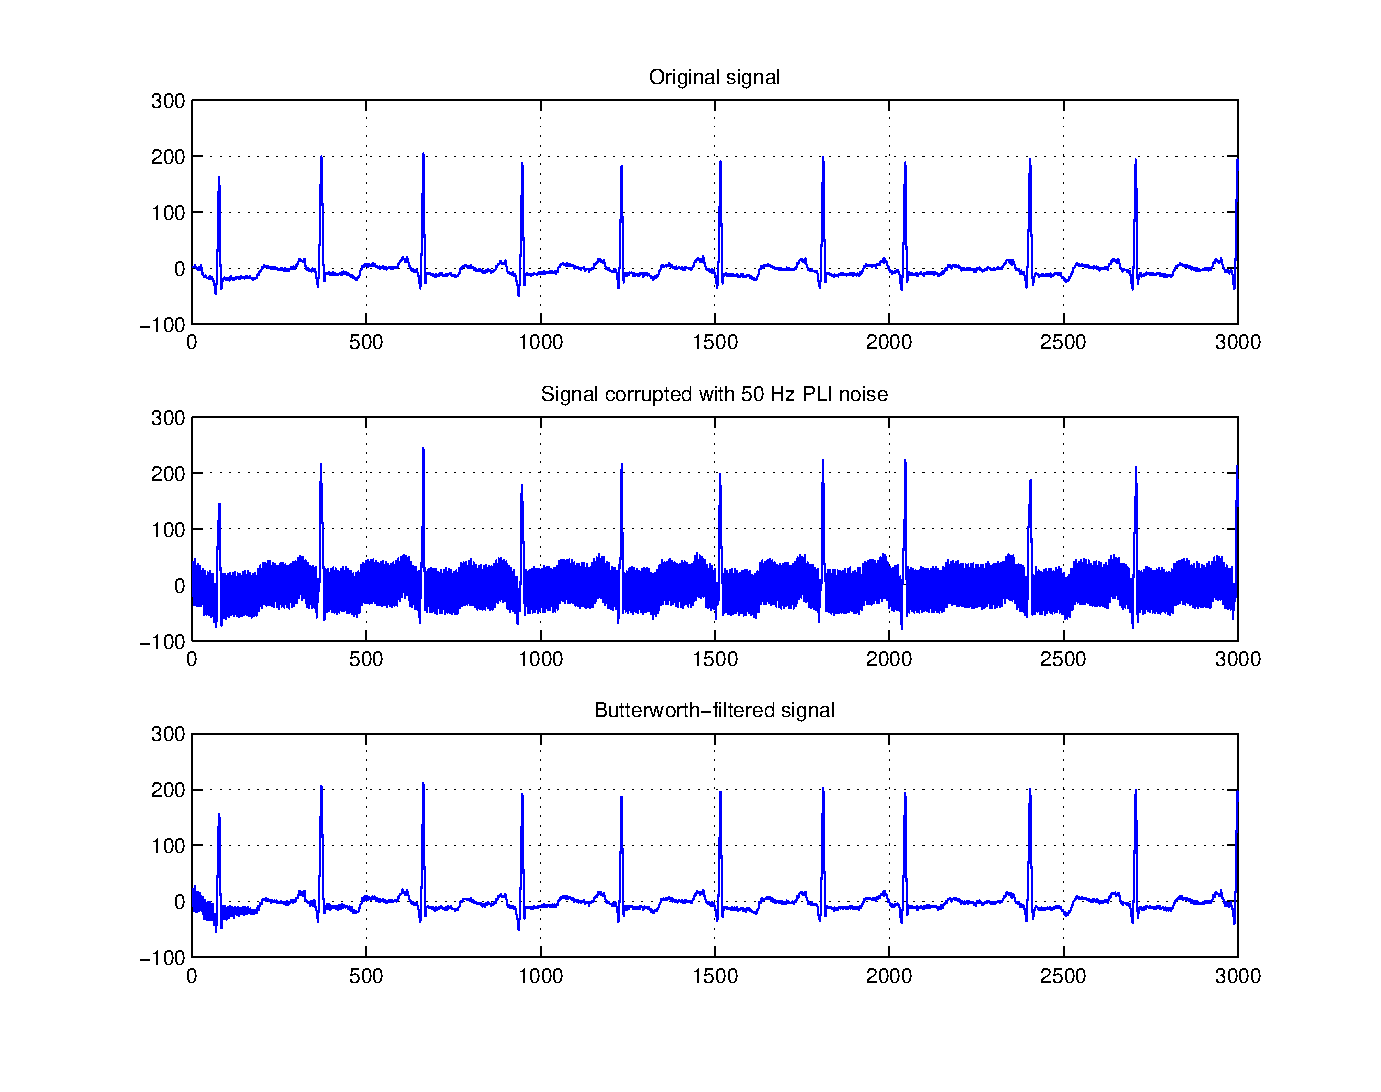
\includegraphics[width=1.05\textwidth]{ECG_BASELINE/figures/50hz.eps}
\caption{Zestawienie sygnałów: przed zaszumieniem, sygnału zaszumionego oraz wyjścia filtru Butterwortha dla szumu sieciowego 50 Hz}
\label{fig:50hz_comparison}
\end{figure}

\begin{figure}[H]
\centering
	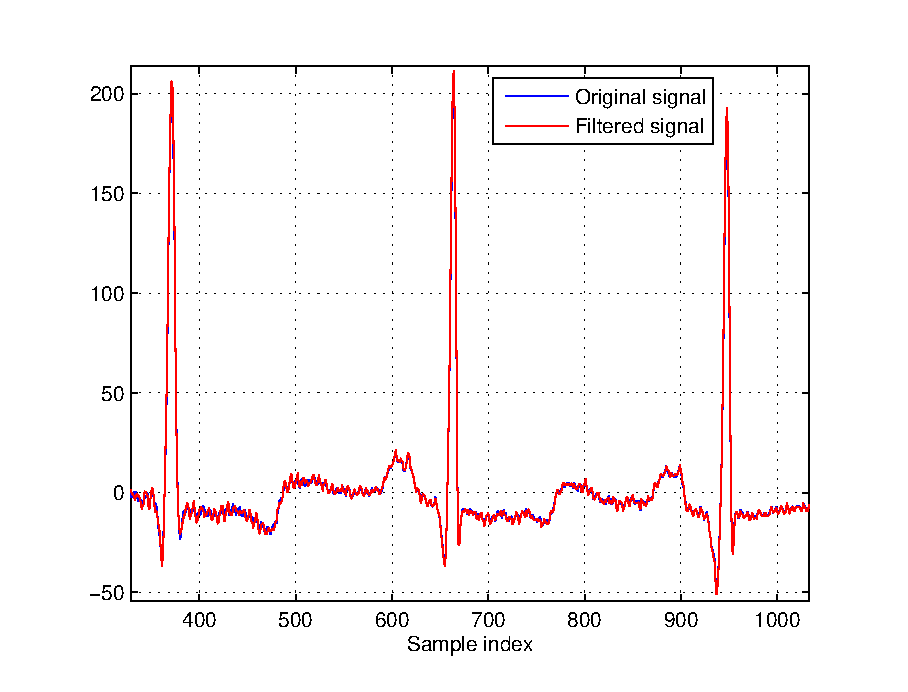
\includegraphics[width=\textwidth]{ECG_BASELINE/figures/50hz_zoom.eps}
\caption{Porównanie wyników filtracji Butterwortha do usuwania szumu sieciowego 50 Hz z sygnałem przed zaszumieniem}
\label{fig:50hz_zoom}
\end{figure}


\subsubsection{Filtr Kalmana}
Rysunek ~\ref{fig:KalmanOutput} przedstawia przykładowy efekt działania rozszerzonego filtru Kalmana, zaś ~\ref{fig:KalmanSNR} - zależność między stosunkiem sygnału użytecznego danych wejściowych i wyjściowych metody. W celu uzyskania mierzalnych wyników, do sygnału wejściowego z usuniętą izolinią dodawano szum biały o zadanej mocy. Zaobserwowano znaczną poprawę sygnału po przeprowadzeniu filtracji, co ma swój wymiar zarówno jakościowy, jak i ilościowy. 

\begin{figure}[H]
\centering
	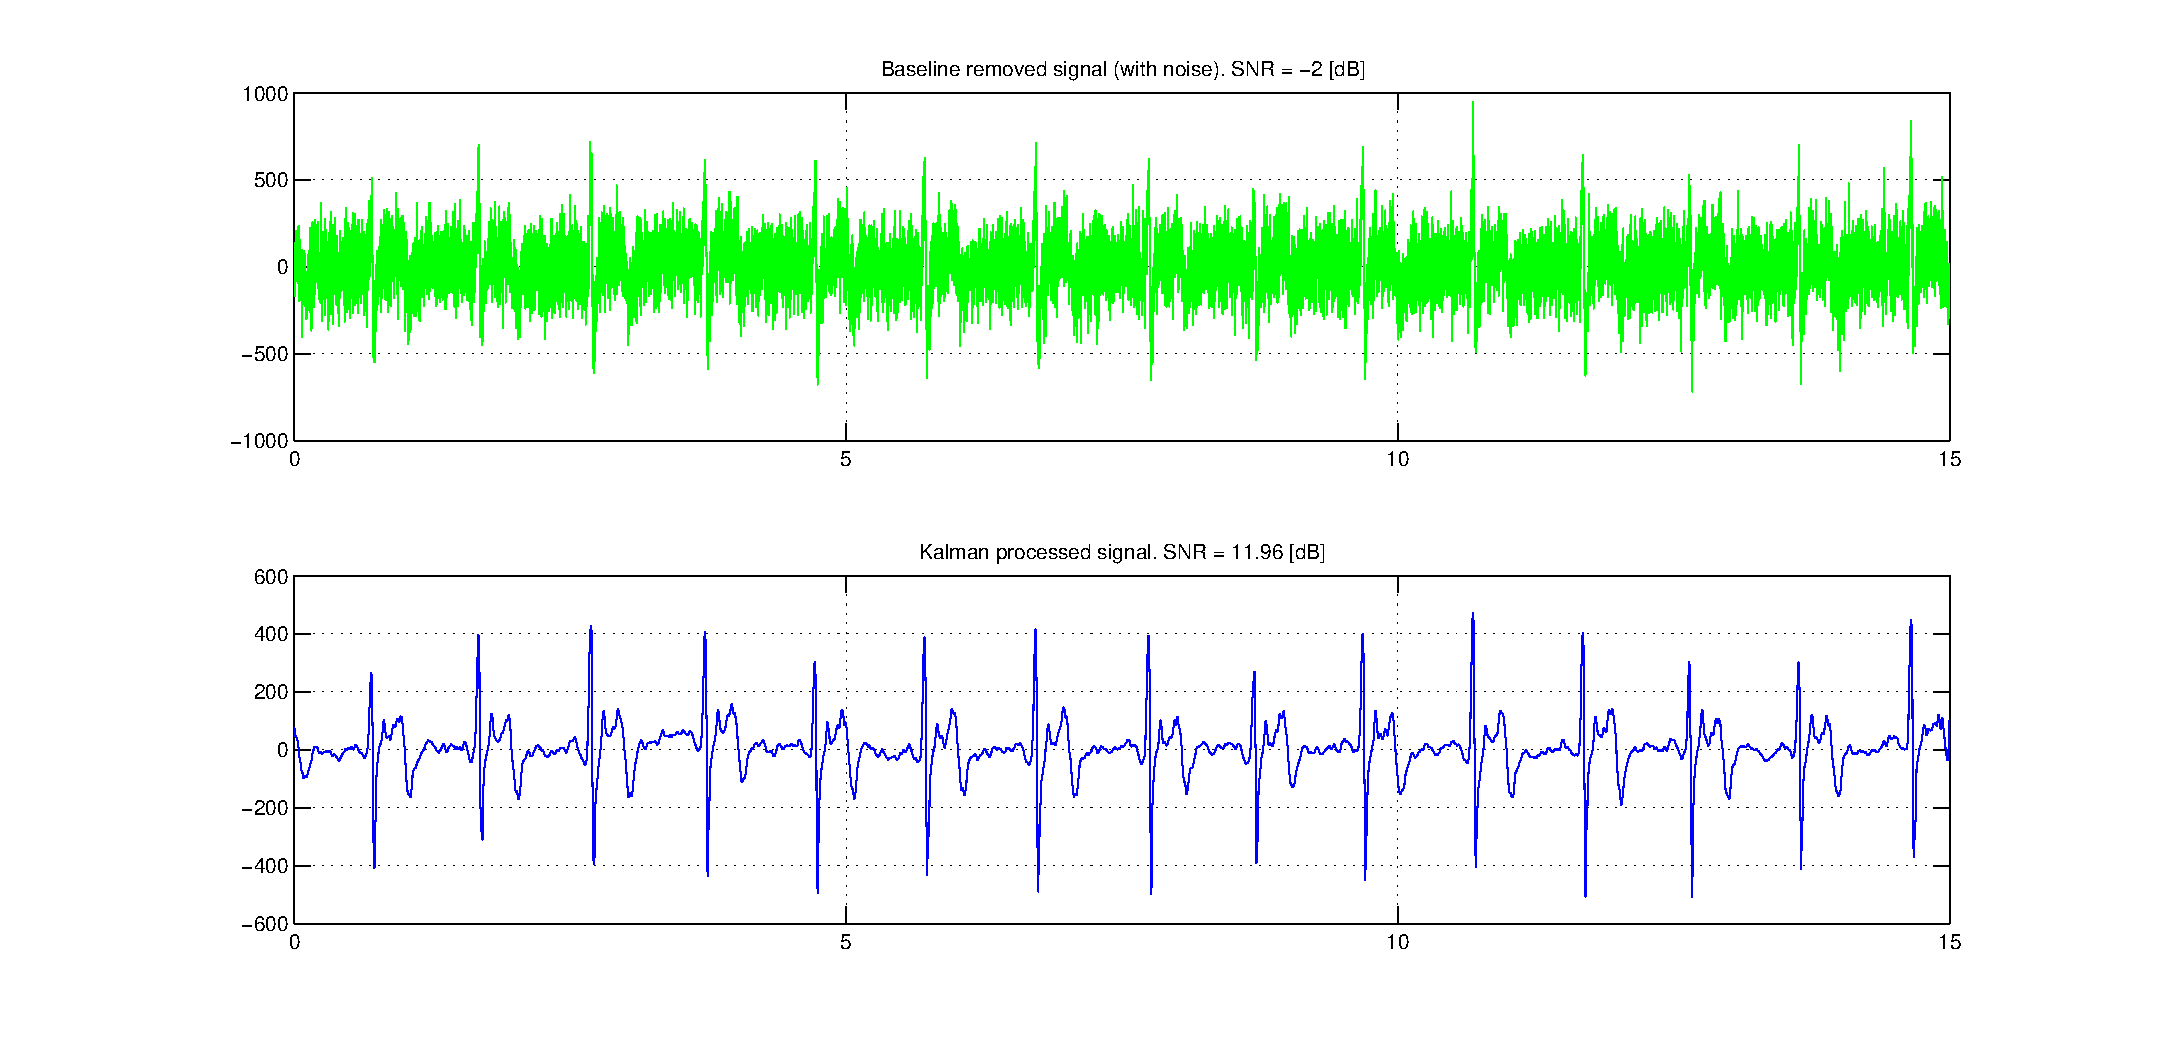
\includegraphics[width=\textwidth]{ECG_BASELINE/figures/hardCoreNoise.eps}
\caption{Wynik filtracji sygnału EKG za pomocą rozszerzonego filtru Kalmana}
\label{fig:KalmanOutput}
\end{figure}

\begin{figure}[H]
\centering
	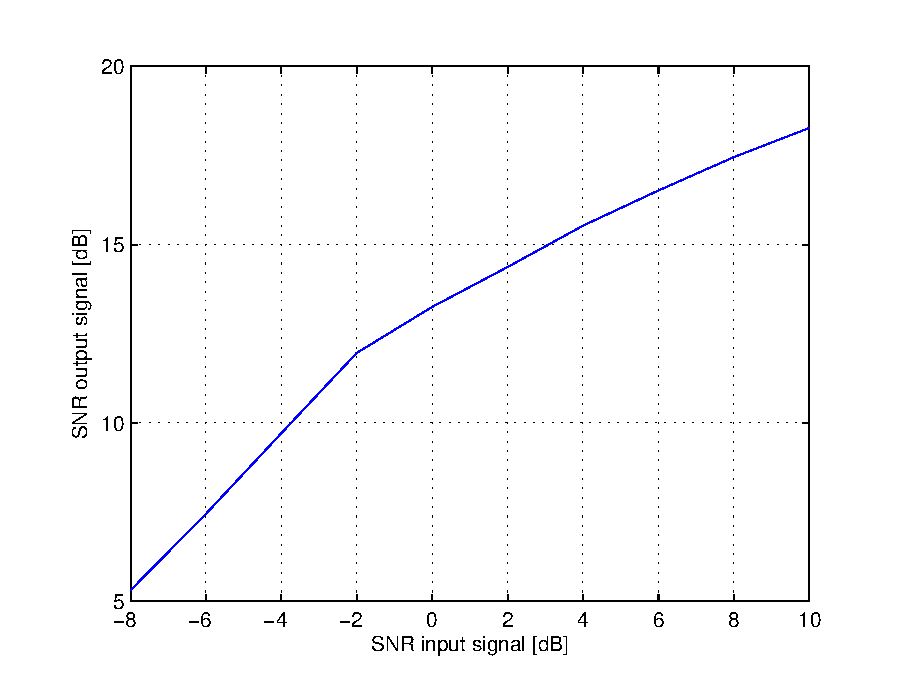
\includegraphics[width=0.9\textwidth]{ECG_BASELINE/figures/snrInOut.eps}
\caption{Zależność między SNR sygnału wejściowego i wyjściowego filtru Kalmana}
\label{fig:KalmanSNR}
\end{figure}



\subsection{Opis implementacji}
Moduł obliczeniowy ECG\_BASELINE zaimplementowany jest w języku C++. Poprawność jego działania testowana była przy użyciu dwóch kompilatorów: Microsoft Visual Studio 2012 oraz gcc w wersji 4.6 (zarówno w wersji MinGW, jak i przeznaczonej dla systemów GNU/Linux).

W module wykorzystane zostały dwie biblioteki zewnętrzne:

\begin{itemize}
\item Eigen -- biblioteka szablonowa C++ zawierająca implementacje operacji macierzowych
\item ALGLIB -- biblioteka C++ zawierająca implementacje wielu algorytmów numerycznych, transformat itp. 
\end{itemize}

Z biblioteki ALGLIB do określenia parametrów modelu syntetycznego sygnału EKG użyta została metoda Levenberga-Marquardta, zaimplementowana w funkcji \texttt{lsfitfit()} z pliku nagłówkowego \texttt{interpolation.h}. 

Średnia krocząca, filtr Butterwortha i filtr Savitzky'ego-Golay'a zaimplementowane zostały funkcje bezstanowe, jednak w porównaniu do poprzedniej wersji, refaktoryzacji uległ interfejs filtru Butterwortha. Do przechowywania współczynników tego filtru utworzona została nowa klasa, przedstawiona w uproszczony sposób na diagramie~\ref{fig:ButterCoefficients_uml}. Wszystkie pola klasy inicjalizowane są w konstruktorze.

\begin{figure}[H]
\centering
	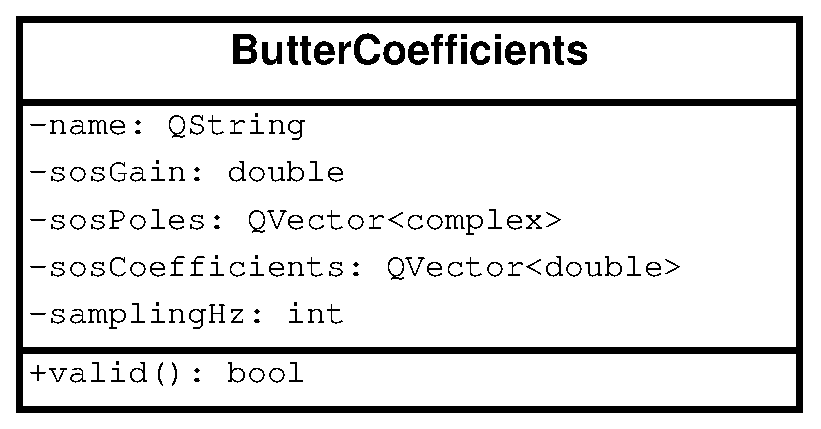
\includegraphics[width=0.4\textwidth]{ECG_BASELINE/figures/ButterCoefficients.eps}
\caption{Diagram UML klasy \textit{ButterCoefficients}}
\label{fig:ButterCoefficients_uml}
\end{figure}

Taka zmiana pozwala na wygodną obsługę wielu zestawów współczynników, a przy użyciu odpowiedniego GUI -- również ich wprowadzanie przez użytkownika. Predefiniowane zestawy współczynników pobiera się przy użyciu funkcji o prototypie \texttt{const QVector<ButterCoefficients>\& predefinedButterCoefficientSets()} zadeklarowanej w pliku nagłówkowym \texttt{butter.h}.

Implementacja filtru Kalmana również udostępnia prosty w użyciu interfejs. Stworzona klasa \textit{KalmanFilter} udostępnia tylko jedną metodę publiczną, zwracającą przefiltrowany sygnał dla surowego wejścia. Metody prywatne odzwierciedlają przedstawiony wyżej algorytm, w razie potrzeby dzielono je na mniejsze części. Powstało w sumie kilkadziesiąt funkcji prywatnych, starano się bowiem, by były one możliwie krótkie i pisane na tym samym poziomie abstrakcji. Metody wykonujące podstawowe operacje na zbiorach danych umieszczono w statycznej klasie \textit{BaseLineUtils}. Poniżej przedstawiono diagram UML klasy \textit{KalmanFilter}, z wyróżnieniem metody publicznej i kilku najważniejszych metod prywatnych. Przedstawione na diagramie atrybuty klasy są ustawiane w jej konstruktorze. Dla filtru Kalmana również utworzono funkcję bezstanową, umożliwiającą filtrowanie podanego wektora próbek.

Podsumowując, dostęp do zaimplementowanych w module metod filtrujących odbywa się poprzez wykorzystanie następujących funkcji bezstanowych, zadeklarowanych w odpowiednich plikach nagłówkowych:

\begin{itemize}

\item \texttt{QVector<double> processMovAvg(const QVector<double> \&signal, int samplingFrequencyHz, double averagingTimeS);}\\ lub \\ \texttt{QVector<double> processMovAvg(const QVector<double>\& signal, int windowSize);}
\item \texttt{QVector<double> processButter(const QVector<double>\& signal, const ButterCoefficients \&coefficients);}
\item \texttt{QVector<double> processSGolay(const QVector<double>\& ecgData, const int deg = 3, const int frame = 500, QVector<double>* baselineModel = 0);}
\item \texttt{QVector<double> processKalman(const QVector<double>\& input, double samplingFrequency);}
\end{itemize}

\begin{figure}[H]
\centering
	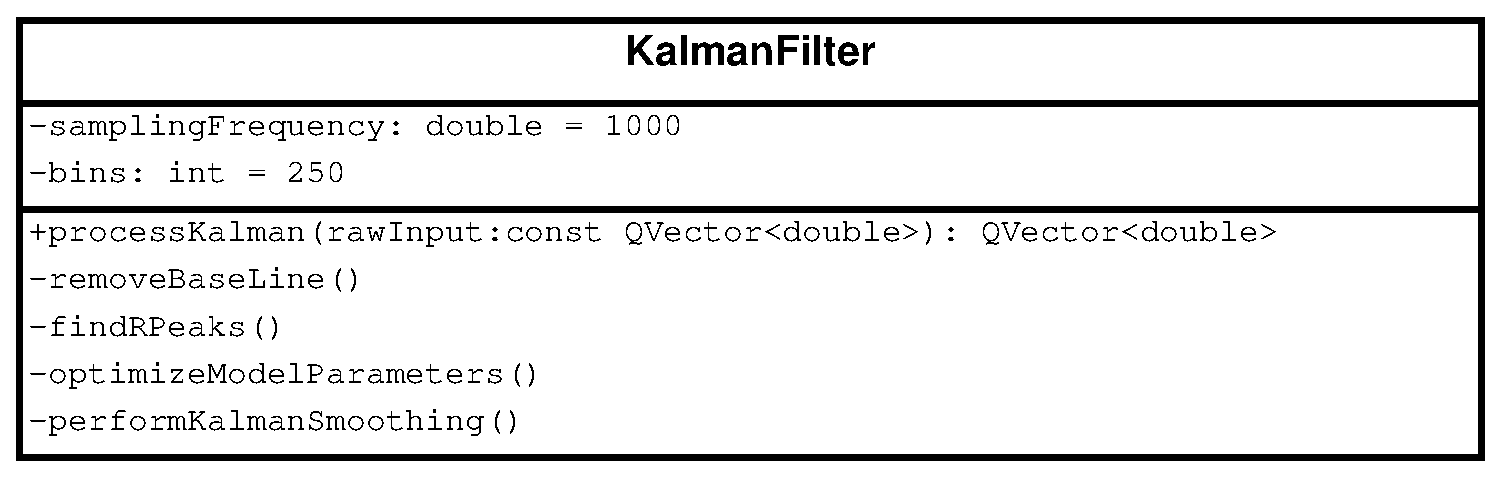
\includegraphics[width=0.7\textwidth]{ECG_BASELINE/figures/KalmanFilter.eps}
\caption{Diagram UML klasy \textit{KalmanFilter}}
\label{KF-UML}
\end{figure}


\subsubsection{Diagramy sekwencji UML}

\begin{figure}[H]
\centering
	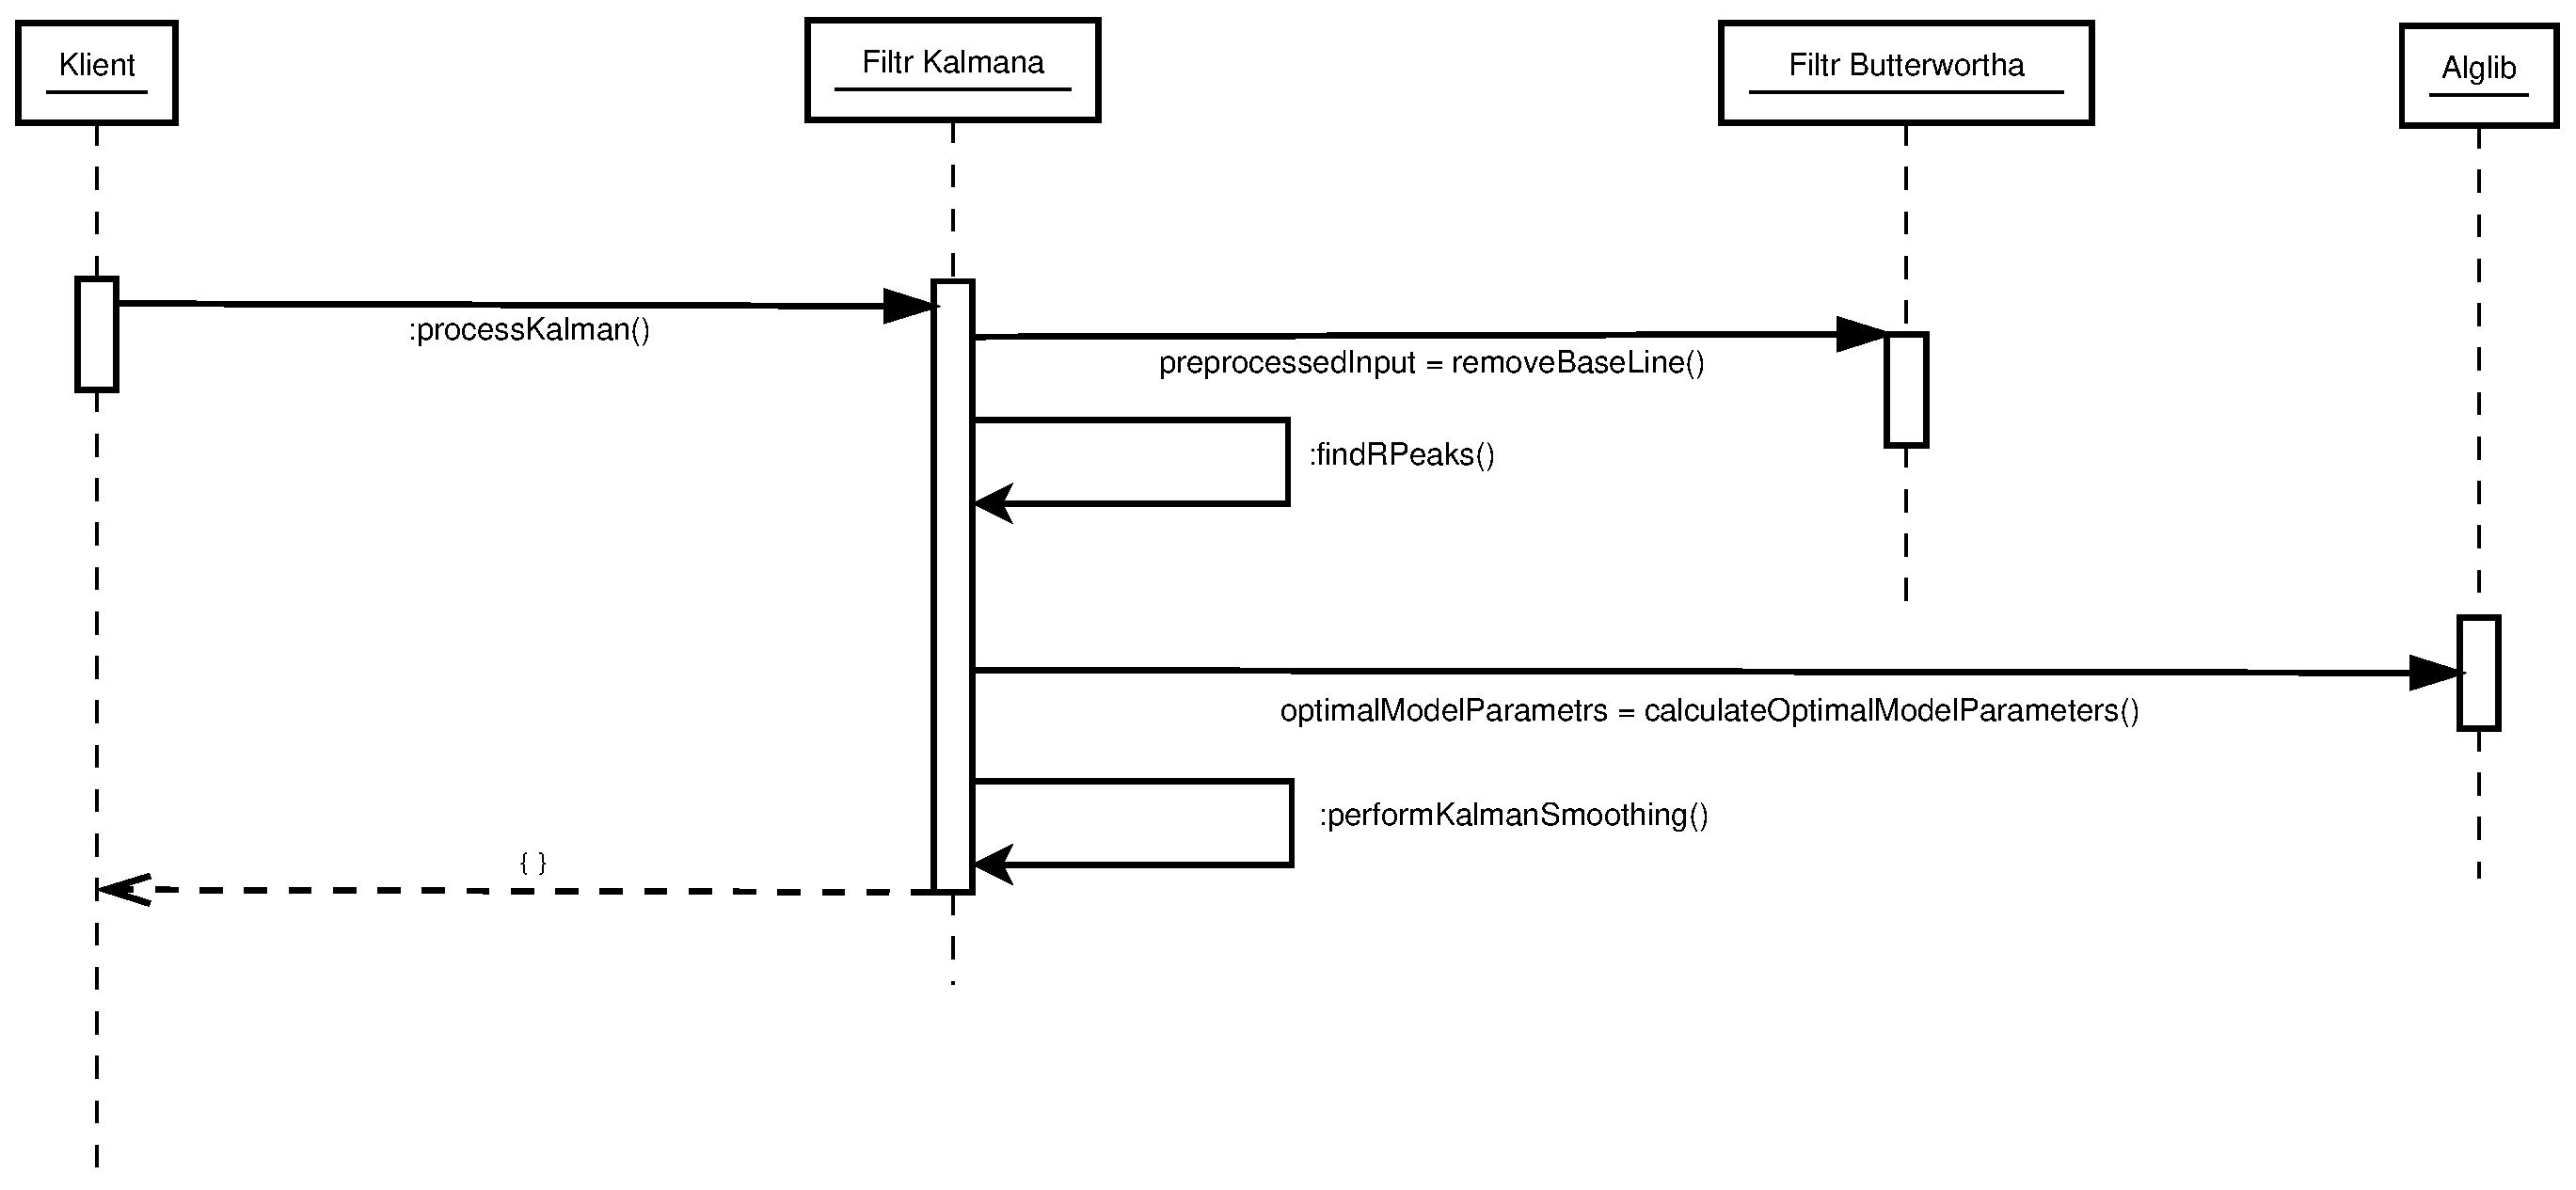
\includegraphics[width=\textwidth]{ECG_BASELINE/figures/KalmanDiagram.eps}
\caption{Diagram sekwencji klasy \textit{KalmanFilter}}
\label{KF-Diagram}
\end{figure}

\begin{figure}[H]
\centering
	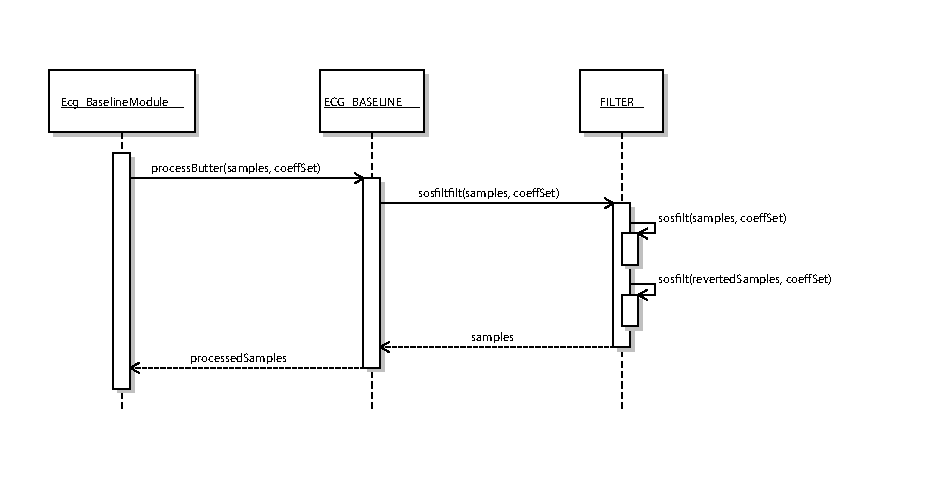
\includegraphics[width=1.1\textwidth]{ECG_BASELINE/figures/butter_seq.pdf}
\caption{Diagram sekwencji dla przypadku użycia filtru Butterwortha.}
\label{MA-seq}
\end{figure}

\begin{figure}[H]
\centering
	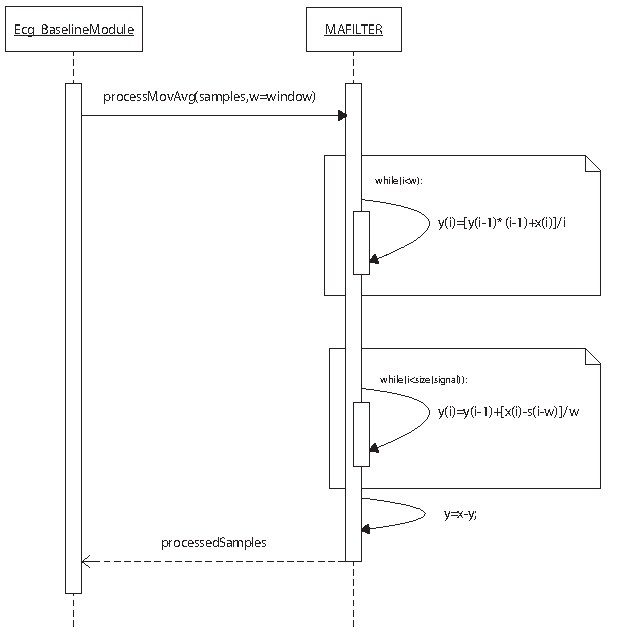
\includegraphics[width=0.8\textwidth]{ECG_BASELINE/figures/ma_seq.pdf}
\caption{Diagram sekwencji dla przypadku użycia średniej kroczącej. Źródło: \cite{Baseline2013}}
\label{MA-seq}
\end{figure}

\begin{figure}[H]
\centering
	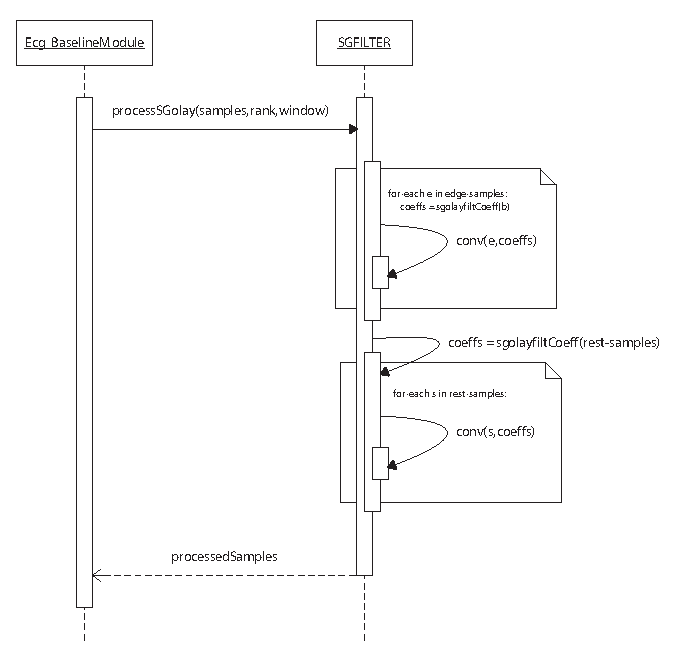
\includegraphics[width=0.8\textwidth]{ECG_BASELINE/figures/sg_seq.pdf}
\caption{Diagram sekwencji dla przypadku użycia filtru Savitzky'ego-Golay'a. Źródło: \cite{Baseline2013}}
\label{MA-seq}
\end{figure}




\subsection{Podsumowanie}
W ramach projektu z powodzeniem zaimplementowano rozszerzony filtr Kalmana dla sygnału EKG, wprowadzono zmiany w interfejsie średniej kroczącej oraz zrefaktoryzowano i dodano nowe zestawy współczynników do filtru Butterwortha. Nowe zestawy współczynników pozwalają na usunięcie z sygnału EKG falowania izolinii oraz szumu sieciowego (50 Hz). 

W przypadku zakłócenia o wielu składowych częstotliwościowych i rozkładzie zbliżonym do normalnego, najlepsze wyniki daje zastosowanie rozszerzonego filtru Kalmana. Jest on znacznie bardziej złożony od typowych filtrów FIR i IIR (jego implementacja w języku C++ wymaga około tysiąca linii kodu) i wymaga znacznie dłuższych obliczeń -- dla zapisu trwającego 30 minut ($f_s = 360 Hz$), czas filtracji wynosi około 45 sekund na komputerze z procesorem klasy Intel i5.

Podsumowując -- usuwanie rzeczywistych zakłóceń w sygnale EKG jest trudne, głównie ze względu na niewielką amplitudę sygnału oraz jego pasmo -- w dużej mierze pokrywające się z pasmem szumów. Problem usunięcia falowania linii izoelektrycznej jest szeroko opisywany w literaturze, zaś zaimplementowane w module ECG\_BASELINE rozwiązania uznać można za spełniające wymagania. Zakłócenia pochodzenia sieciowego (PLI -- \emph{Power Line Interference}) są również niemal całkowicie usuwalne przy użyciu pasmowozaporowych filtrów Butterwortha z odpowiednimi zestawami współczynników. 

\setcounter{secnumdepth}{3}
\section{Moduł R\_PEAKS}
\subsection{Badania literaturowe}

Zadaniem modułu R\_PEAKS jest detekcja załamków R w elektrokardiogramie. Jest to jeden z kluczowych etapów analizy sygnału EKG. Poprawne wykrycie i oznaczenie załamków R umożliwia bowiem wykrycie pozostałych punktów charakterystycznych cyklu pracy serca. Pozwala to dalej np. na przeprowadzenie dokładnej analizy zmienności rytmu serca. Załamki R są częścią tzw. zespołu QRS, który został przedstawiony na rysunku \ref{fig:RPQRS}.
\begin{figure}[H]
\centering

\includegraphics[scale=0.7]{R_PEAKS/img/qrs_class}
\caption{Fragment sygnału EKG z zaznaczonym zespołem QRS (QRS Complex)}
\label{fig:RPQRS}
\end{figure}
Zespół QRS tworzą trzy sąsiadujące ze sobą punkty elektrokardiogramu, które składają się na wychylenie w kształcie wąskiego impulsu. Załamek Q to pierwsze ujemne wychylenie elektrokardiogramu, załamek R to pierwsze dodatnie wychylenie elektrokardiogramu, a załamek S to ostatnie ujemne wychylenie elektrokardiogramu w zespole QRS.

Zespół QRS jest odzwierciedleniem elektrycznej aktywności serca podczas skurczu komorowego. Reprezentuje on pobudzenie, czyli depolaryzację komór serca. Zespół QRS charakteryzuje się najwyższym wychyleniem i najkrótszym czasem trwania, co sprawia, że posiada on szerokie widmo częstotliwościowe. Charakterystyczny kształt tego zespołu oraz czas jego pojawiania się dostarcza najwięcej informacji diagnostycznych o bieżącym stanie serca i dlatego też jest punktem wyjściowym do klasyfikacji schematu cyklu sercowego. Służy też jako podstawa do automatycznego określania rytmu. Wykrycie zespołu QRS dostarcza podstawowych zasad i informacji dla prawie wszystkich automatycznych algorytmów analizy EKG. Czas trwania oraz wysokość zespołu QRS jest zależny od wielu czynników. Przyjmuje się jednak, że dla dorosłego i zdrowego człowieka średni czas trwania zespołu powinien wynosić od 0,06 s do 0,10 s. Wysokość sygnału zaś powinna mieścić się między 0,7 mV a 1,8 mV.

Detekcja załamków R wciąż jest przedmiotem wielu badań oraz licznych prac naukowych. Nie opracowano do tej pory metody, która gwarantowałaby stuprocentową skuteczność działania. Istnieją jednak algorytmy, które zapewniają ponad dziewięćdziesięciodziewięcio procentową skuteczność. Najpowszechniej stosowanym algorytmem jest algorytm Pan-Tompkins. Bazuje on na analizie odpowiednio przefiltrowanego oraz uśrednionego sygnału EKG. Algorytm ten łatwo adaptuje się do dynamiki sygnału. Dzięki temu jest bardzo skuteczny nawet w przypadku nieregularnej pracy serca. Ponadto metoda ta bardzo dobrze spisuje się w systemach czasu rzeczywistego. Wśród pozostałych algorytmów dużą popularnością cieszą się algorytmy oparte na przekształceniach Hilberta oraz transformacji falkowej. Przedmiotem obecnych badań są też metody, które łączyłyby te dwa algorytmy. Pozostałymi algorytmami detekcji załamków R są między innymi metody oparte na sieciach neuronowych, algorytmach genetycznych czy procesach stochastycznych.
\subsection{Koncepcja proponowanego rozwiązania}

W trakcie realizacji modułu R\_PEAKS zdecydowano się na implementację trzech algorytmów detekcji załamków R:
\begin{itemize}
\item algorytm Pan - Tompkins,
\item algorytm bazujący na przekształceniach Hilberta,
\item algorytm bazujący na transformacji falkowej.
\end{itemize}
\subsubsection{Algorytm Pan - Tompkins}

Algorytm ten można podzielić na dwa etapy. Pierwszym jest odpowiednie przygotowanie sygnału poprzez przefiltrowanie go oraz późniejsze jego uśrednienie. Drugim etapem jest znajdowanie załamków R we wcześniej przygotowanym sygnale. Na rysunku \ref{fig:RPPTA} przedstawiono schemat blokowy pierwszego etapu algorytmu.
\begin{figure}[H]
\centering
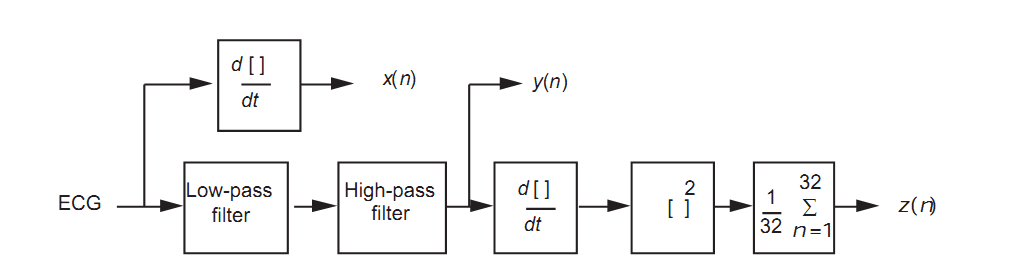
\includegraphics[scale=0.4]{R_PEAKS/img/pan_tompkins_alg}
\caption{Kolejne etapy algorytmu Pan - Tompkins przygotowujące sygnał do detekcji załamków R}
\label{fig:RPPTA}
\end{figure}
\begin{enumerate}[I.]
\item Przepuszczenie sygnału przez filtry dolno i górnoprzepustowy.
\item Różniczkowanie

Celem różniczkowania sygnału jest wytłumienie komponentów niskoczęstotliwościowych oraz wzmocnienie komponentów wysokoczęstotliwościowych charakterystycznych dla zespołów QRS. W tej fazie skorzystano z różniczkowania pięciopunktowego opisanego wzorem:
\begin{equation}
y(nT)=\frac{1}{8}[-x(nT-2T)-2x(nT-T)+2x(nT+T)+x(nT+2T)]
\end{equation}
\item Potęgowanie

Potęgowanie sygnału ma na celu jeszcze większe wzmocnienie próbek sygnału odpowiadających zespołom QRS oraz wytłumienie pozostałych próbek sygnału. Ponadto potęgowania zapewnia nieujemność sygnału.
\begin{equation}
y(nT)=[x(nT)]^2
\end{equation}
\item Całkowanie

Całkowanie sygnału w ruchomym oknie ma na celu jego wygładzenie oraz uzyskanie pojedynczej "fali" w obrębie zespołu QRS. Całkowanie sygnału wyraża się następującym wzorem:
\begin{equation}
y(nT)=\frac{1}{N}\sum\limits_{i=nT-NT}^{nT} x(i)
\end{equation}
Gdzie N to szerokość okna, którą należy odpowiednio dobrać w zależności od częstotliwości próbkowania. Należy mieć tu na uwadze fakt, że zbyt duża wielkość okna spowoduje zlanie się dwóch fal, a zbyt mała z kolei skutkować będzie utworzeniem zbyt dużej liczby fal.
\item Progowanie i detekcja załamków R

W trakcie pracy algorytmu odnajdywane są kolejne maksima lokalne, którą mogą być oznaczone jako załamek R lub jako szum. Wykorzystywane są przy tym dwa progi: THRESHOLD1 i THRESHOLD2. Są one na bieżąco aktualizowane na podstawie estymaty amplitudy załamków R (SPK) i szumu (NPK). Dodatkowo wykorzystywana jest technika searchback z parametrem RRMISSEDLIMIT, który wyznaczany jest na podstawie różnic między kolejnymi załamkami R. Poniżej przedstawiono reguły detekcji załamków R:

\begin{algorithmic}
\If {załamek R wykryto w czasie maksymalnie 200 ms od ostatniego załamka R \textbf{AND} amplituda nowego załamka jest mniejsza od poprzedniego wykrytego}
    \State odrzuć załamek
\ElsIf {nowy załamek R wykryto w czasie ponad 200 ms, a mniej niż 360 ms od ostatniego załamka \textbf{AND} nachylenie sygnału przy nowym maksimum jest przynajmniej równe połowie nachylenia dla poprzedniego maksimum}
    \State dodaj załamek
\ElsIf {wartość wykrytego maksimum jest większa niż THRESHOLD1}
	\State dodaj załamek
\ElsIf{załamek R nie został wykryty przez okres RRMISSEDLIMIT \textbf{AND} w ciągu tego czasu zostały znalezione maksima większe niż THRESHOLD2}
	\State dodaj jako załamek największe znalezione maksimum
\EndIf
\end{algorithmic}
%\begin{itemize}
%\item Jeżeli nowy załamek R wykryto w czasie maksymalnie 200 ms od ostatniego załamka R i amplituda nowego załamka jest mniejsza od poprzedniego wykrytego to ten załamek jest odrzucany.
%\item Jeżeli nowy załamek R wykryto w czasie ponad 200 ms, a mniej niż 360 ms od ostatniego załamka sprawdza się, czy maksymalne nachylenie sygnału przy nowym maksimum jest przynajmniej równe połowie nachylenia dla poprzedniego maksimum. Jeżeli nie, to przyjmuje się, że maksimum jest szumem, np. załamkiem T.
%\item Jeżeli wartość wykrytego maksimum jest większa niż THRESHOLD1, to uznaje się to maksimum za załamek R, w przeciwnym razie jest to szum.
%\item Technika searchback: Jeżeli załamek R nie został wykryty przez okres RRMISSEDLIMIT, a w ciągu tego czasu zostały znalezione maksima większe niż THRESHOLD2, to największe z nich traktowane jest jako załamek R.
%\end{itemize}
W takcie działania algorytmu konieczna jest aktualizacja progów. Są one aktualizowane na podstawie wartości parametrów SPK i NPK, których początkowe wartości są następujące:
\begin{itemize}
\item SPK = średnia z ośmiu maksimów z pierwszych ośmiu sekund badania,
\item NPK = 0.
\end{itemize}
Wartości tych parametrów są aktualizowane w następujący sposób:
\begin{algorithmic}
\If {załamek R został wykryty za pomocą porównania z THRESHOLD1}
    \State $SPK \gets 0.125 PEAK + 0.875 SPK$
\ElsIf {załamek R został wykryty za pomocą porównania z THRESHOLD2}
	\State $SPK \gets 0.250 PEAK + 0.750 SPK$
\Else 
	\State $NPK \gets 0.125 PEAK + 0.875 NPK$
\EndIf
\end{algorithmic}
%\begin{itemize}
%\item jeżeli załamek R został wykryty za pomocą porównania z THRESHOLD1 
%\newline
%SPK = 0.125 PEAK + 0.875 SPK,
%\item jeżeli załamek R został wykryty za pomocą porównania z THRESHOLD2 
%\newline
%SPK = 0.250 PEAK + 0.750 SPK,
%\item jeżeli został wykryty szum
%\newline
%NPK = 0.125 PEAK + 0.875 NPK
%\end{itemize}
Progi natomiast są aktualizowane w następujący sposób:
\newline
THRESHOLD1 = NPK+ 0.25 (SPK-NPK)
\newline
THRESHOLD2 = 0.5 THRESHOLD1

Interwały pomiędzy kolejnymi załamkami R obliczane są jako różnica wystąpienia ich czasów. Jeżeli interwał jest większy niż 0.92 RRAVERAGE2 i mniejszy niż 1.12 RRAVERAGE2, bufor interwałów jest aktualizowany o ostatnią wartość interwału i obliczana jest nowa wartość RRAVERAGE2. Wartość RRMISSEDLIMIT używana w technice searchback jest równa 1.66 RRAVERAGE2 i stanowi czas, w którym poszukiwane są zaginione maksima.
\end{enumerate}
\subsubsection{Algorytm bazujący na przekształceniach Hilberta}
Przekształcenie Hilberta to przekształcenie liniowe. Funkcji x(t) przypisywana jest funkcja xh(t) postaci:
\begin{equation}
x_H = \mathcal{H}\{x(t)\}=\frac{1}{\pi}\int_{-\infty}^\infty \frac{x(\lambda)d\lambda}{t-\lambda}
\end{equation}
W powyższym wzorze występuje dość trudna do wyliczenia niewłaściwa całka Riemanna. W takiej sytuacji należy skorzystać z transformaty Fouriera. Wzór na przekształcenie Hilberta przyjmuje wtedy postać:
\begin{equation}
x_H(t)=Im \{ \mathcal{F}^{-1} \{ \mathcal{F} \{ x(t) \}(\omega)\cdot (-j)sgn(\omega)\}  \}
\end{equation}
W pierwszym etapie algorytmu dokonujemy transformacji Hilberta całego sygnału EKG. Następnie na podstawie sygnałów x(t) oraz xh(t) wyznacza się tzw. obwiednię sygnału postaci:
\begin{equation}
\mathcal{B}(t)=\sqrt{x(t)^2+x_H(t)^2}
\end{equation}
Po wyznaczeniu obwiedni sygnału należy przystąpić do etapu progowania.

\begin{enumerate}[I.]
\item Wyznaczenie początkowej wartości progu

Pierwsza wartość progu powinna być nieco mniejsza niż maksymalna wartość sygnału B(t). Najczęściej spotykana wartość progu to ok. 0,9 wartości maksymalnej sygnału B(t).
\item Wyznaczenie wartości o jaką należy zmniejszać próg w kolejnych iteracjach

Jeżeli za M1 przyjęto maksymalną wartość sygnału B(t), a za M2 wartość minimalną tego sygnału to wartość o jaką należy zmniejszać próg w każdej iteracji wyraża się następującym wzorem:
\begin{equation}
fi=0,01\cdot M1 \cdot x \cdot mantysa(M1-M2)
\end{equation}
\item Wyznaczenie załamków

W tym kroku należy wyliczyć ile próbek sygnału B(t) jest większych od obecnego progu. Jeżeli liczba próbek powyżej progu jest większa od ilości próbek w poprzedniej iteracji to należy zmniejszyć próg o wartość fi i ponownie policzyć próbki powyżej progu. Jeżeli ilość próbek powyżej progu się nie zmieniła to należy przerwać etap progowania.

Ostatnim etapem jest detekcja załamków R. Wyznaczone w etapie progowania próbki powyżej progu będą występować w grupach. W każdej z tych grup znajdować się będzie próbka o największej amplitudzie, która będzie szukanym załamkiem R.
\end{enumerate}
\subsubsection{Algorytm bazujący na transformacji falkowej}

Falki (z ang. wavelet) – rodziny funkcji zbioru liczb rzeczywistych w zbiór liczb rzeczywistych, z których każda jest wyprowadzona z funkcji-matki (z tzw. funkcji macierzystej) za pomocą przesunięcia i skalowania:
\begin{equation}
\psi_{j,k}(t)=\psi(2^j +k)
\end{equation}
gdzie: j,k – liczby całkowite, $\psi$ – funkcja - matka, $\psi_{j,k}$ – falka o skali j i przesunięciu k (zwana też funkcją falkową). Funkcje te dążą do zera lub po prostu wynoszą zero dla argumentów dążących do nieskończoności. Ponadto funkcje te mają energię skupioną w jednym miejscu tzn.
\begin{equation}
\int\limits_{-\infty}^{\infty} \psi(t)dt=0
\end{equation}
Transformacja falkowa dla sygnałów ciągłych jest przekształceniem całkowym:
\begin{equation}
\tilde{s}_{\Psi}=\frac{1}{\sqrt{a}}\int\limits_{-\infty}^{\infty}s(t)\Psi(\frac{t-b}{a})dt
\end{equation}
gdzie:
\begin{itemize}
\item a - parametr skali
\item b - parametr przesunięcia
\item s(t) - sygnał badany zależny od czasu t
\item $\Psi$ - funkcja falkowa
\item $\tilde{s} _\Psi$ - współczynnik falkowy zależny od parametrów a i b
\item $\Psi(\frac{t-b}{a})$ - jądro przekształcenia
\end{itemize}
Zastosowanie transformacji falkowej pozwala rozłożyć sygnał na kilka subpasm (rysunek \ref{fig:RPWS}). Następnie dobiera się odpowiednie subpasma i rekonstruuje sygnał. Tak uzyskany sygnał poddaje się takiej samej procedurze progowania i detekcji załamków R jak w przypadku wcześniej opisywanego algorytmu wykorzystującego przekształcenia Hilberta.
\begin{figure}[H]
\centering
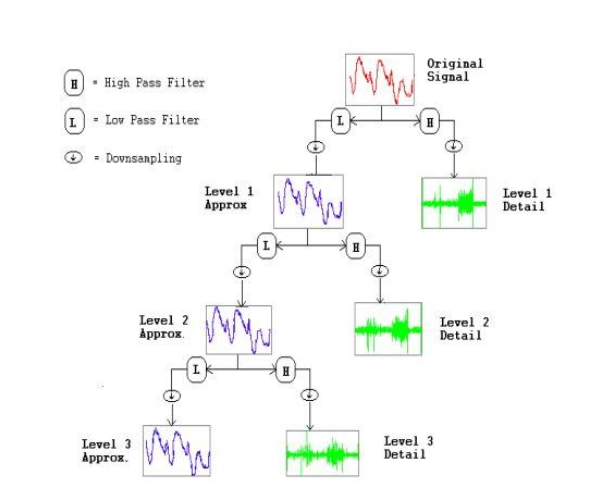
\includegraphics[scale=0.6]{R_PEAKS/img/wavelet_schema}
\caption{Dekompozycja sygnału na subpasma za pomocą transformacji falkowej}
\label{fig:RPWS}
\end{figure}

Działanie algorytmu można przedstawić w następujących krokach:
\begin{enumerate}[I.]
\item Dwukrotna dekompozycja oryginalnego sygnału z wykorzystaniem transformacji falkowej.
\item Wyszukanie próbki o największej wartości w zdekomponowanym sygnale.
\item Znalezienie wszystkich próbek o wartości nie mniejszej niż 30\% wartości próbki znalezionej w poprzednim kroku.
\item Filtracja próbek, które zostały wykryte w poprzednim kroku w celu odrzucenia tych, które należą do tego samego załamka R.
\item Znalezienie indeksów wyszukanych próbek w sygnale po transformacji i przemnożenie ich razy 4 w celu znalezienia w przybliżeniu indeksów próbek w sygnale oryginalnym, które zostały sklasyfikowane jako załamki R.
\item Wyszukanie faktycznego indeksu próbki w oryginalnym sygnale poprzez przeszukanie odpowiedniego przedziału oryginalnego sygnału wokół próbki o indeksie znalezionym w poprzednim kroku.
\end{enumerate}
\subsection{Rezultaty i wnioski}
Zaimplementowane metody w większości przypadków działają dobrze i poprawnie wykrywają załamki R. Ewentualny błąd wynosi co najwyżej kilka próbek. W przypadku sygnałów dosyć zniekształconych zdarzają się sytuacje, że zostały wykryte nadmiarowe załamki R, bądź niektóre z nich nie zostały w ogóle wykryte.

Należy jednak nadmienić, iż metody detekcji załamków R, Pan - Tompkins oraz bazująca na transformacie Hilberta, które zostały zaimplementowane w roku poprzednim przez kolegów Pawła Kasperczyka i Kamila Pękalę działają poprawnie. Z tego powodu zostały również wykorzystane w tegorocznym projekcie. Zostały wprowadzone jednak drobne modyfikacje związane z dopasowaniem tych metod pod API tegorocznego projektu, jak również pewne modyfikacje w sposobie zwracania rezultatów obliczeń funkcji składowych klasy reprezentującej moduł oraz pewne zmiany kosmetyczne związane z formatowaniem kodu. Konsekwencją wynikającą z wykorzystania zaimplementowanych już metod jest to, że są pewne różnice pomiędzy proponowanym w wcześniej rozwiązaniem a rozwiązaniem zastosowanym w programie.

W zaimplementowanej metodzie bazującej na transformacji Hilberta został zastosowany podział sygnału na przedziały. Transformacja dokonywana jest zatem na fragmencie sygnału, po czym otrzymane rezultaty sklejane są w całość. Zgodnie z informacjami zawartymi w raporcie z zeszłorocznego projektu, daje to lepsze rezultaty, niż obliczenia dokonywane na całym sygnale bez podziału na przedziały. Kolejną różnicą jest to, że nie jest obliczany pierwiastek kwadratowy, który występuje we wzorze na obwiednią sygnału. Upraszcza to obliczenia. Podyktowane jest to faktem, iż liczba rzeczywista o większej wartości ma również większy pierwiastek kwadratowy. Również sama metoda detekcji załamków R jest nieco inna niż proponowana w jednym z wcześniejszych rozdziałów. Dokonywana ona jest na podstawie przeglądu fragmentu tablicy \textit{diff} zawierającej posortowane malejąco elementy, które są większe niż $\frac{1}{21}$ maksymalnej wartości z tej. Elementy te są wkładem transformaty Hilberta w obwiednię sygnału, obliczone na podstawie wspomnianego wyżej, uproszczonego wzoru niezawierającego pierwiastka kwadratowego. Próbka sygnału wejściowego, która odpowiada aktualnie przeglądanemu elementowi tablicy, jest odpowiednio daleko od poprzednio zakwalifikowanych jako załamek R próbek, jest również traktowana jako szukany załamek. W przeciwnym przypadku jest odrzucana. Minimalna odległość między załamkami jest oszacowana na podstawie założenia, iż maksymalna częstotliwość pracy serca wynosi 220 uderzeń na minutę. Wyznaczona odległość pomnożona jest jeszcze przez współczynnik wynoszący 0,8. Szerokość fragmentu sygnału poddawanego transformacji Hilberta przyjęta została jako 200 sekund.

Bardzo ważnym elementem detekcji załamków R jest uzyskanie do analizy dobrze przefiltrowanego sygnału, pozbawionego dużych zakłóceń i szumów. Podczas testów poprawności działania modułu został przeprowadzony eksperyment polegający na detekcji załamków R w sygnale nie poddanym filtracji. Metoda Pan - Tompkins mimo wszystko dała w miarę dobre rezultaty, natomiast metoda bazująca na transformacji Hilberta kompletnie nie poradziła sobie z wykryciem pików. Prawdopodobnie główną przyczyną tego faktu jest obecność prostej i odwrotnej transformaty Fouriera w zaimplementowanej metodzie. Metoda oparta na transformacji falkowej, w zaimplementowanym w module algorytmie, wyszukuje załamki, których wartość przekracza pewien ustalony próg wyznaczony w oparciu o próbkę o największej wartości. Z tego powodu obecność zakłóceń o zbyt dużej wartości może powodować zakwalifikowanie tych zakłóceń jako nadmiarowe załamki.

Z racji, iż stosowane algorytmy przeważnie wykrywają trochę mniejszą liczbę załamków niż wynosi ona w rzeczywistości, ciężko było dokonać analizy różnic pomiędzy wynikami zwróconym przez algorytm a wynikami referencyjnymi w sposób automatyczny, przy wykorzystaniu programu. Dla wybranych sygnałów EKG zostały narysowane wykresy z naniesionymi, referencyjnymi i wyznaczonymi przez algorytmy, załamkami R. Sygnał oryginalny był filtrowany przy pomocy filtru Butterwortha. Nie zostały przeprowadzone testy dla innych metod filtracji w oparciu o założenie, że każda z tych metod daje poprawne rezultaty i wyniki detekcji załamków R powinny być podobne dla każdej z metod filtrowania sygnału.
\subsubsection{Analiza rezultatów działania modułu oraz porównanie algorytmów detekcji załamków R na podstawie wybranych sygnałów}
\begin{itemize}
\item Sygnał nr 105
%
%
%
%
Sygnał o numerze 105 został wybrany do analizy efektów działania modułu ze względu na jego ciekawy kształt w drugiej połowie.

\begin{table}[H]
\centering
\label{105peaks}
\caption{Załamki R dla sygnału 105}
\begin{tabular}{|l|c|}
\hline
\multicolumn{2}{|c|}{Sygnał nr 105}\\
\hline
Referencyjne & 2691 \\ \hline
Hilbert & 2607 \\ \hline
Pan - Tompkins & 2554 \\ \hline
Transformata falkowa & 2587 \\ \hline
\end{tabular}
\end{table}

\begin{enumerate}[I.]
\item Algorytm bazujący na transformacji Hilberta

Na wykresie \ref{fig:105HC} zaznaczone zostały czerwonymi kółkami wykryte przez algorytm załamki R, natomiast kwadratami koloru czarnego naniesione są piki referencyjne. Taki sposób oznaczania załamków jest przyjęty dla pozostałych wykresów.

Można odnieść wrażenie, że różnice między załamkami referencyjnymi i tymi znalezionymi przez algorytm są dosyć duże. Jednak po dokonaniu szybkiej analizy wykresu \ref{fig:105HF} nasuwa się wniosek, że różnica nie jest duża, rzędu kilku próbek, a wrażenie dużych różnic spowodowane jest stromym nachyleniem załamka. Można również zauważyć, że wykryte zostały pewne nadmiarowe piki. W związku z tym, należy się spodziewać, że wiele pików zostało również pominiętych. Wynika to z faktu, że sumaryczna ilość załamków wykrytych przez algorytm jest ciut mniejsza niż ilość załamków referencyjnych. Można również stwierdzić, iż załamki referencyjne nie są również idealne. Może to być podyktowane ewentualnymi opóźnieniami powstałymi np. w przypadku filtracji sygnału.
\newpage
\begin{figure}[H]
\centering
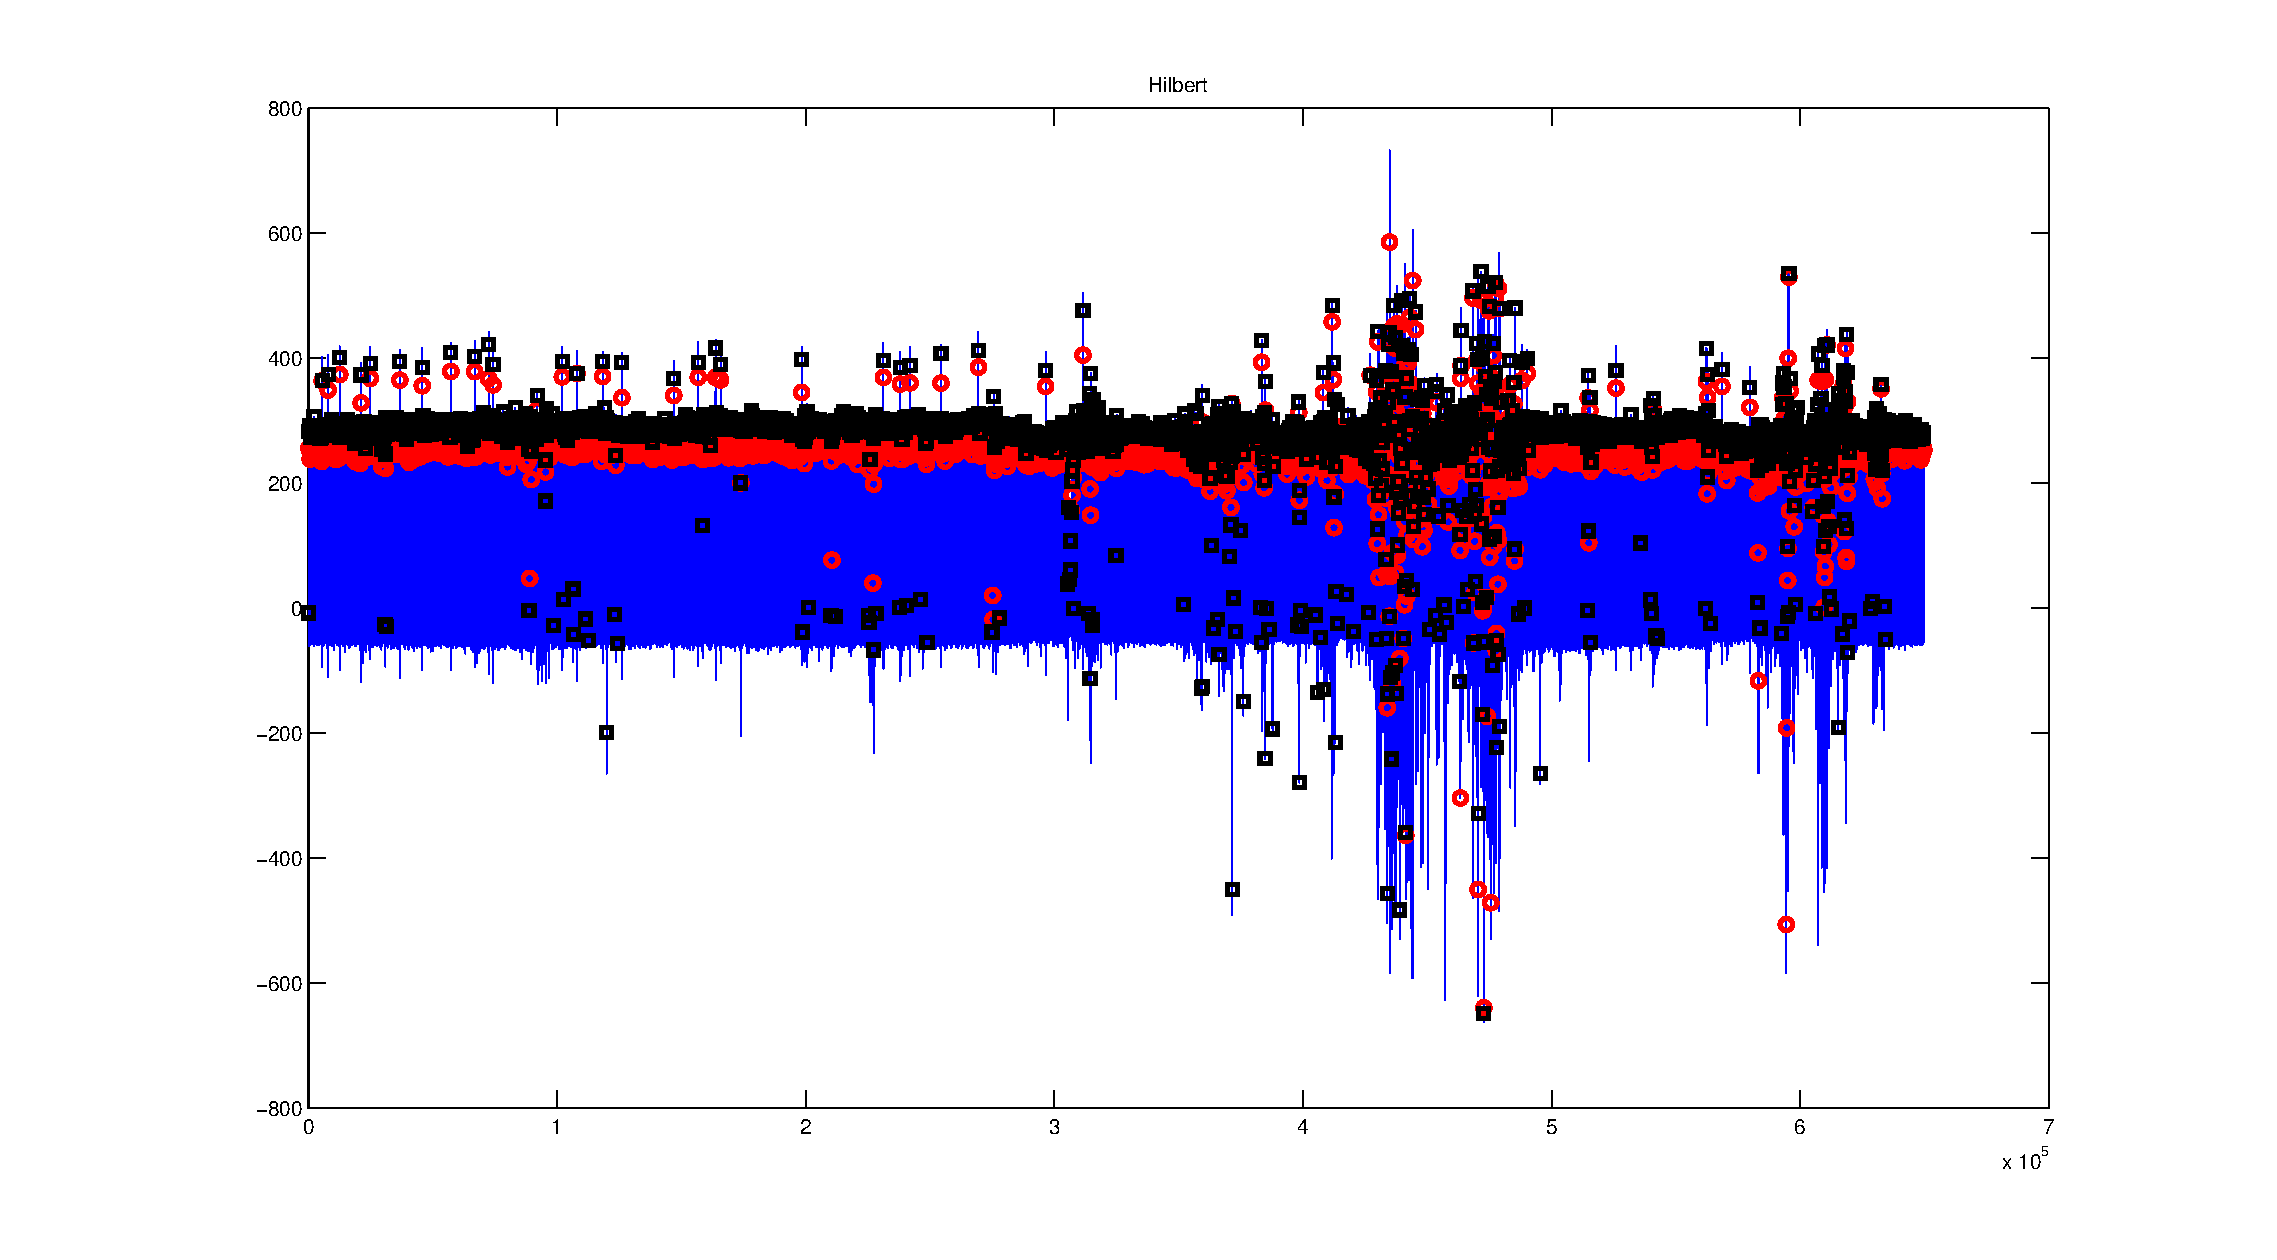
\includegraphics[scale=0.35]{R_PEAKS/wektorowe/105_hilbert_calosc.eps}
\caption{Sygnał nr 105 z naniesionymi pikami R - Hilbert}
\label{fig:105HC}
\end{figure}

\begin{figure}[H]
\centering
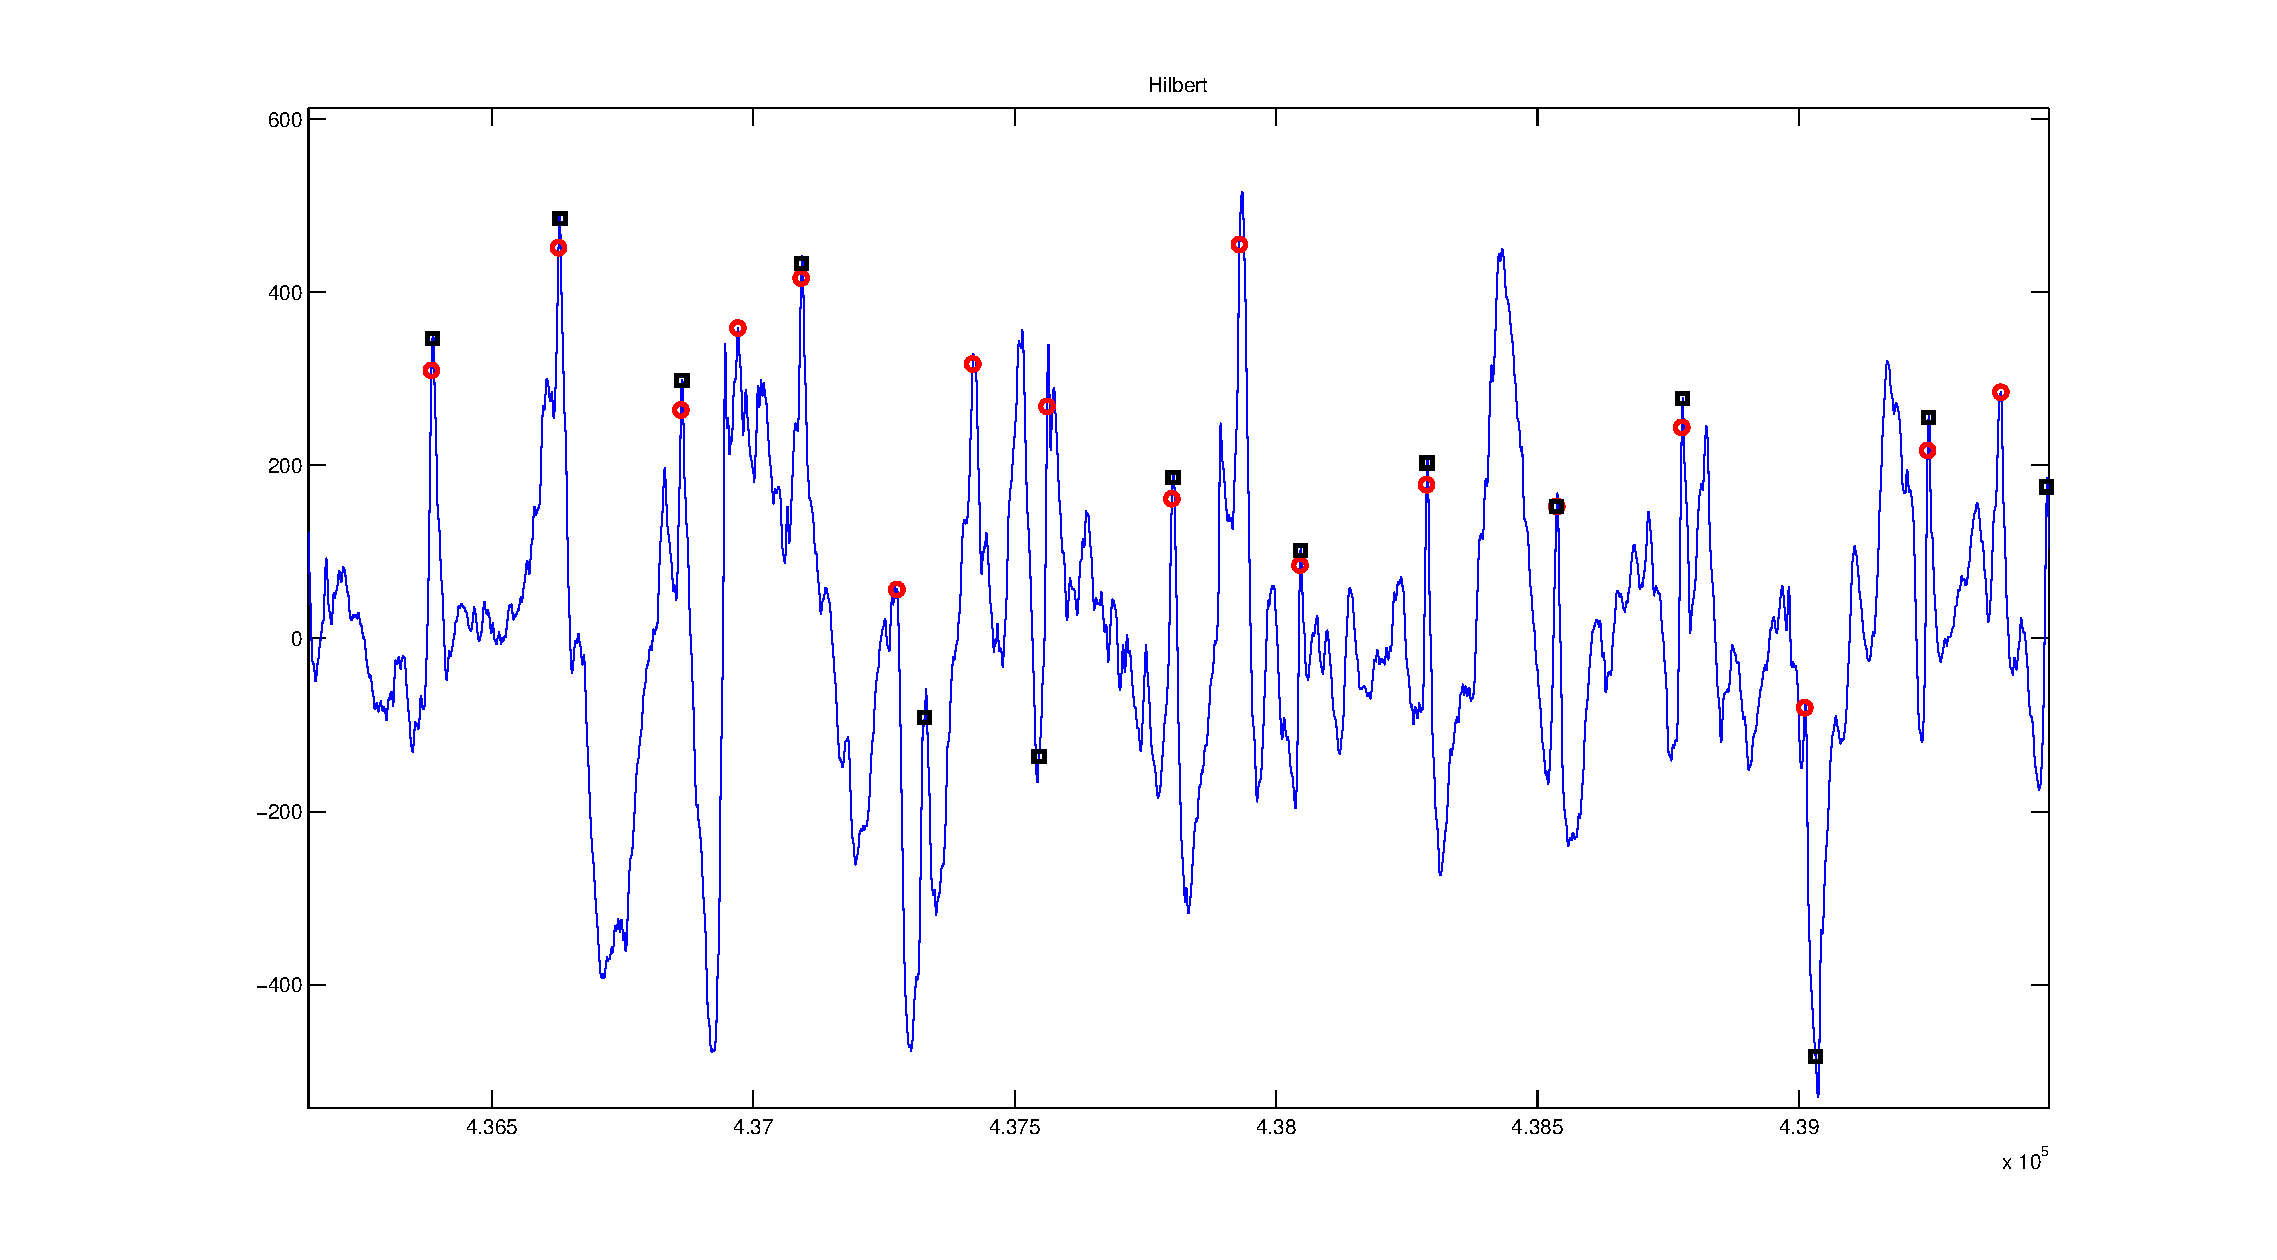
\includegraphics[scale=0.35]{R_PEAKS/wektorowe/105_hilbert_fragment.eps}
\caption{Fragment sygnału nr 105 - Hilbert}
\label{fig:105HF}
\end{figure}
%
%
%
\newpage
\item Algorytm Pan - Tompkins

Dla sygnału o nr. 105, wynik działania algorytmu Pan - Tompkins wydają się być lepsze niż dla algorytmu, który bazuje na przekształceniu Hilberta. Wprawdzie można zauważyć na rysunku \ref{fig:105PTC}, że jest całkiem sporo załamków niewykrytych, lecz te, które zostały znalezione, różnią się niewiele od tych referencyjnych. Analizując fragment sygnału widać, że niejednokrotnie załamki znalezione na drodze działania algorytmu pokrywają się z referencyjnymi, lub różnią się od nich bardzo mało. Podobnie jak w przypadku poprzedniej metody, ilość wykrytych załamków jest nieco mniejsza niż ich faktyczna liczba.

\begin{figure}[H]
\centering
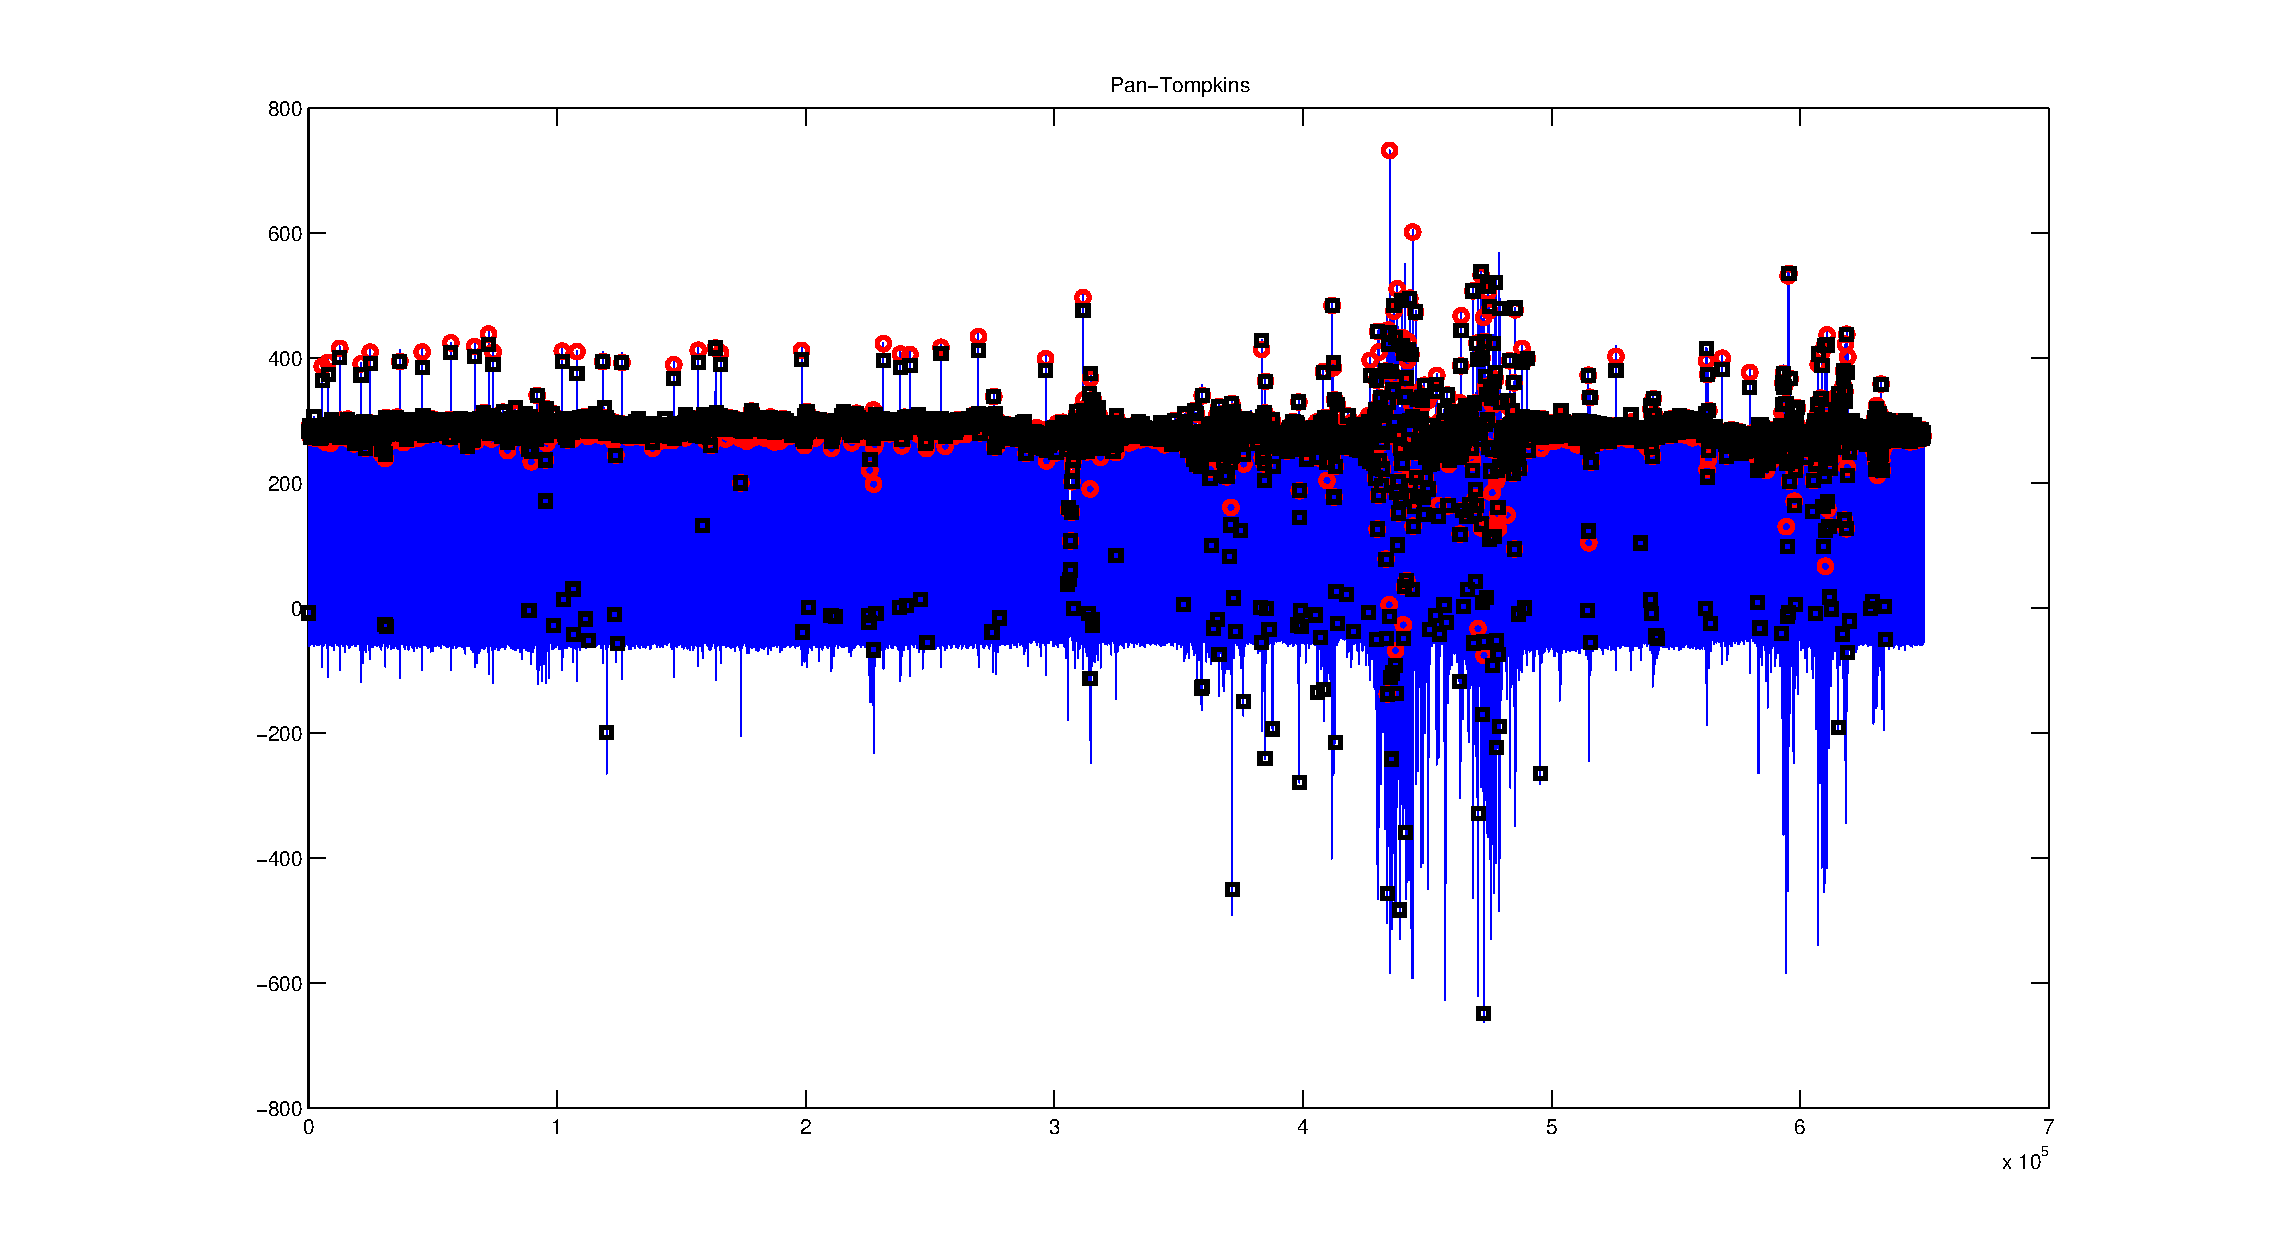
\includegraphics[scale=0.35]{R_PEAKS/wektorowe/105_pan_calosc.eps}
\caption{Sygnał nr 105 z naniesionymi pikami R - Pan - Tompkins}
\label{fig:105PTC}
\end{figure}
\newpage
\begin{figure}[H]
\centering
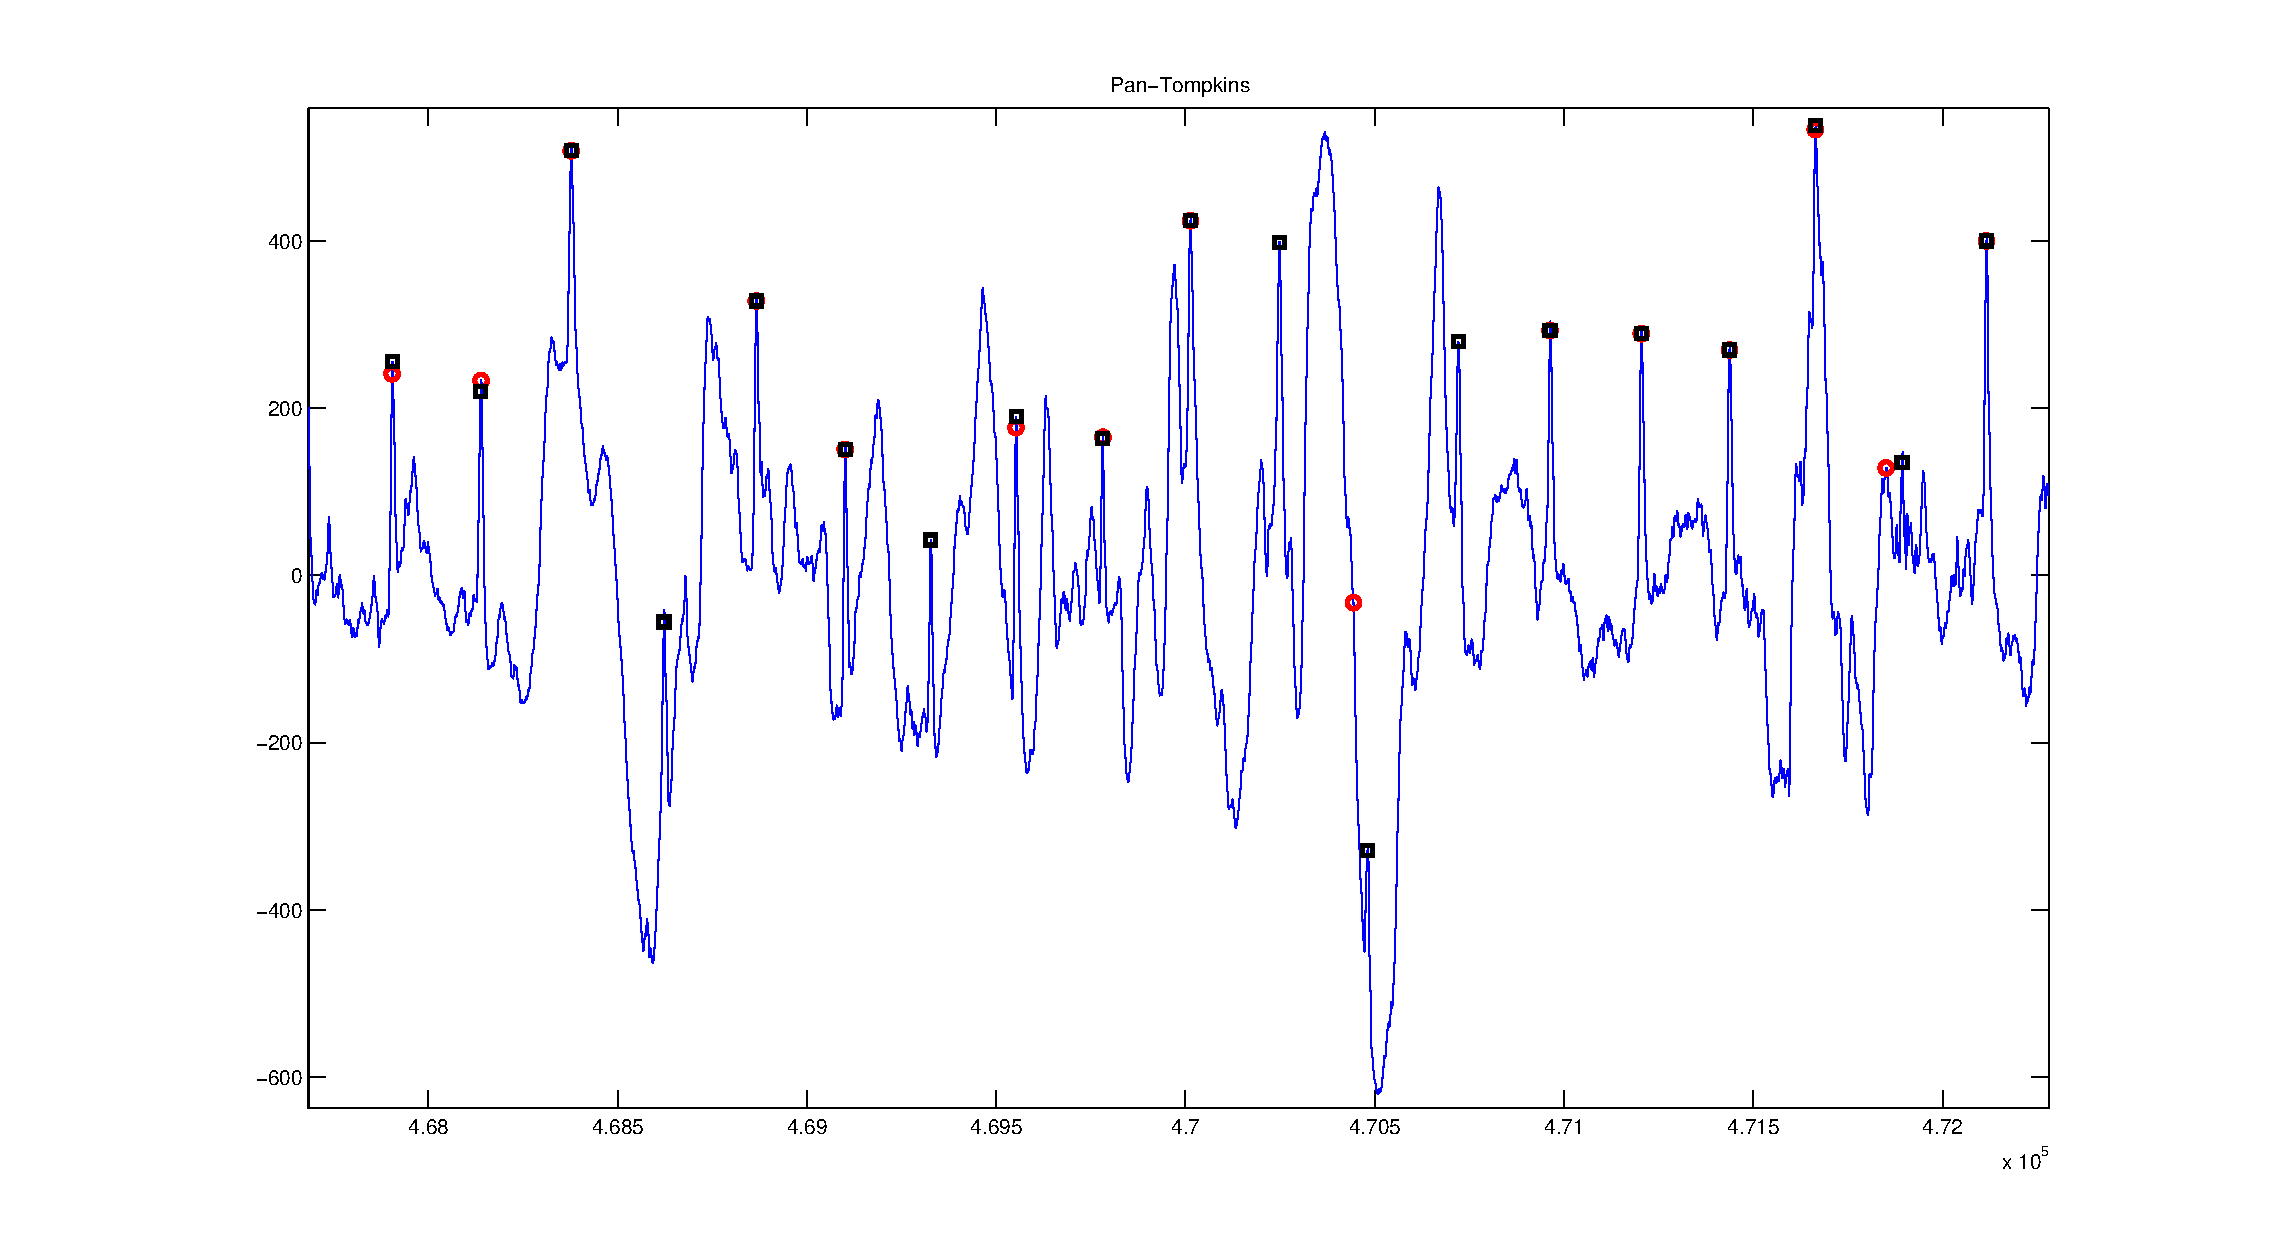
\includegraphics[scale=0.35]{R_PEAKS/wektorowe/105_pan_fragment.eps}
\caption{Fragment sygnału nr 105 - Pan - Tompkins}
\label{fig:105PTF}
\end{figure}
%
%
%
%
\item Algorytm bazujący na transformacji falkowej

Specyfika działania tego algorytmu powoduje, że za przyczyną widocznego na rysunku \ref{fig:105WC}, mniej więcej w dwóch trzecich sygnału wysokiemu załamkowi, dosyć dużo załamków R nie zostało wykrytych. Natomiast w przypadku załamków, które zostały odnalezione, widoczna jest mała różnica w stosunku do załamków referencyjnych. Analiza fragmentu sygnału (rys. \ref{fig:105WF}) pokazuje, że często piki wykryte przez algorytm są lepsze od referencyjnych, lub pokrywają się z nimi.
\newpage
\begin{figure}[H]
\centering
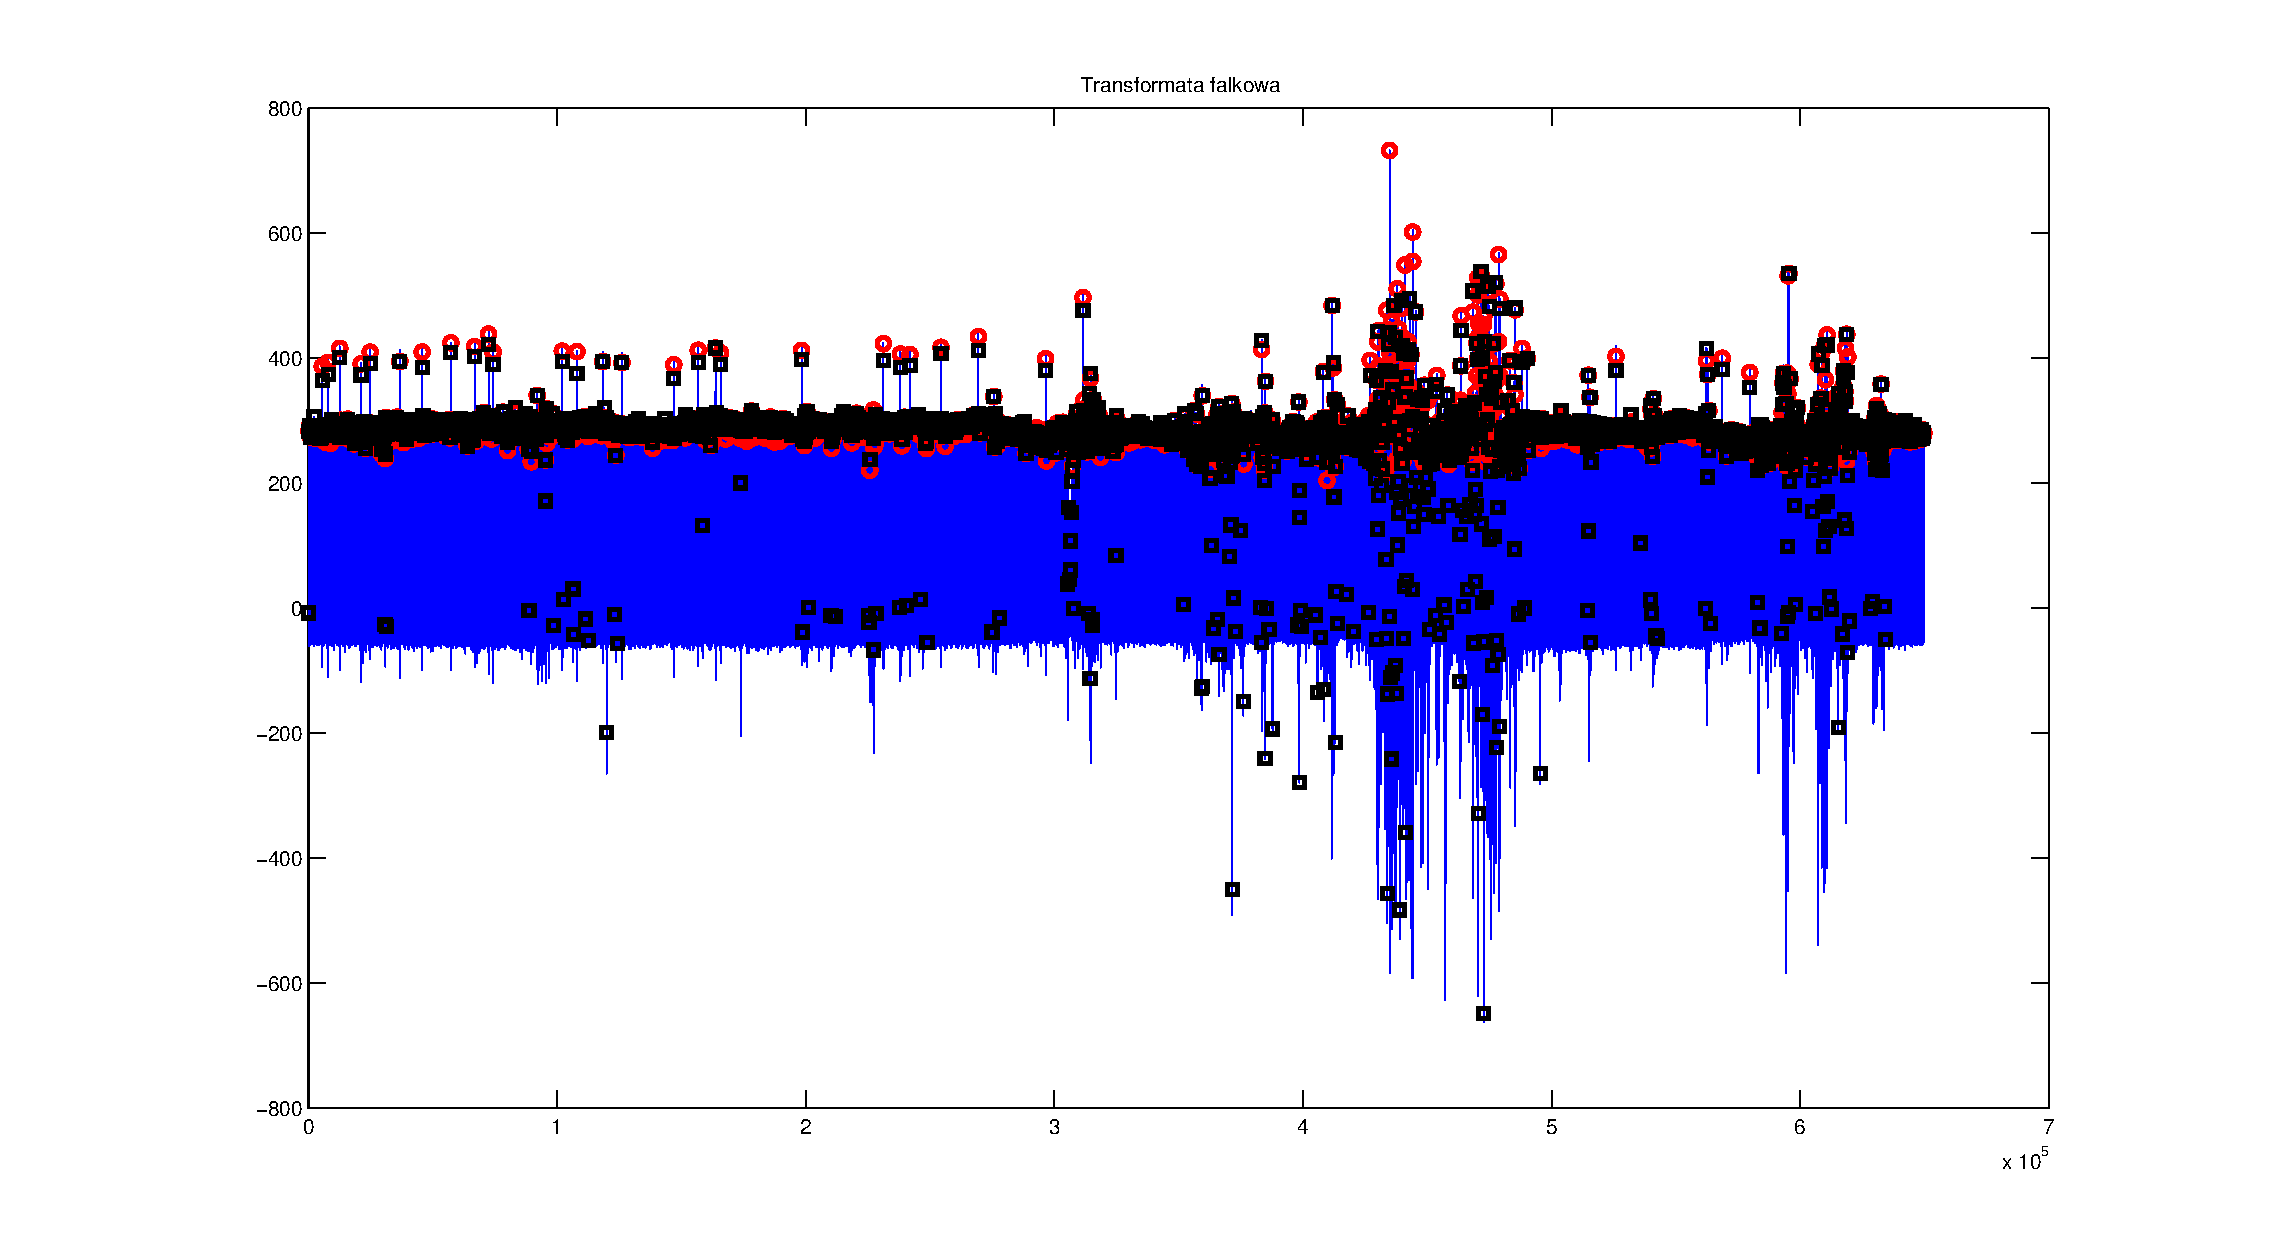
\includegraphics[scale=0.35]{R_PEAKS/wektorowe/105_falka_calosc.eps}
\caption{Sygnał nr 105 z naniesionymi pikami R - transformata falkowa}
\label{fig:105WC}
\end{figure}

\begin{figure}[H]
\centering
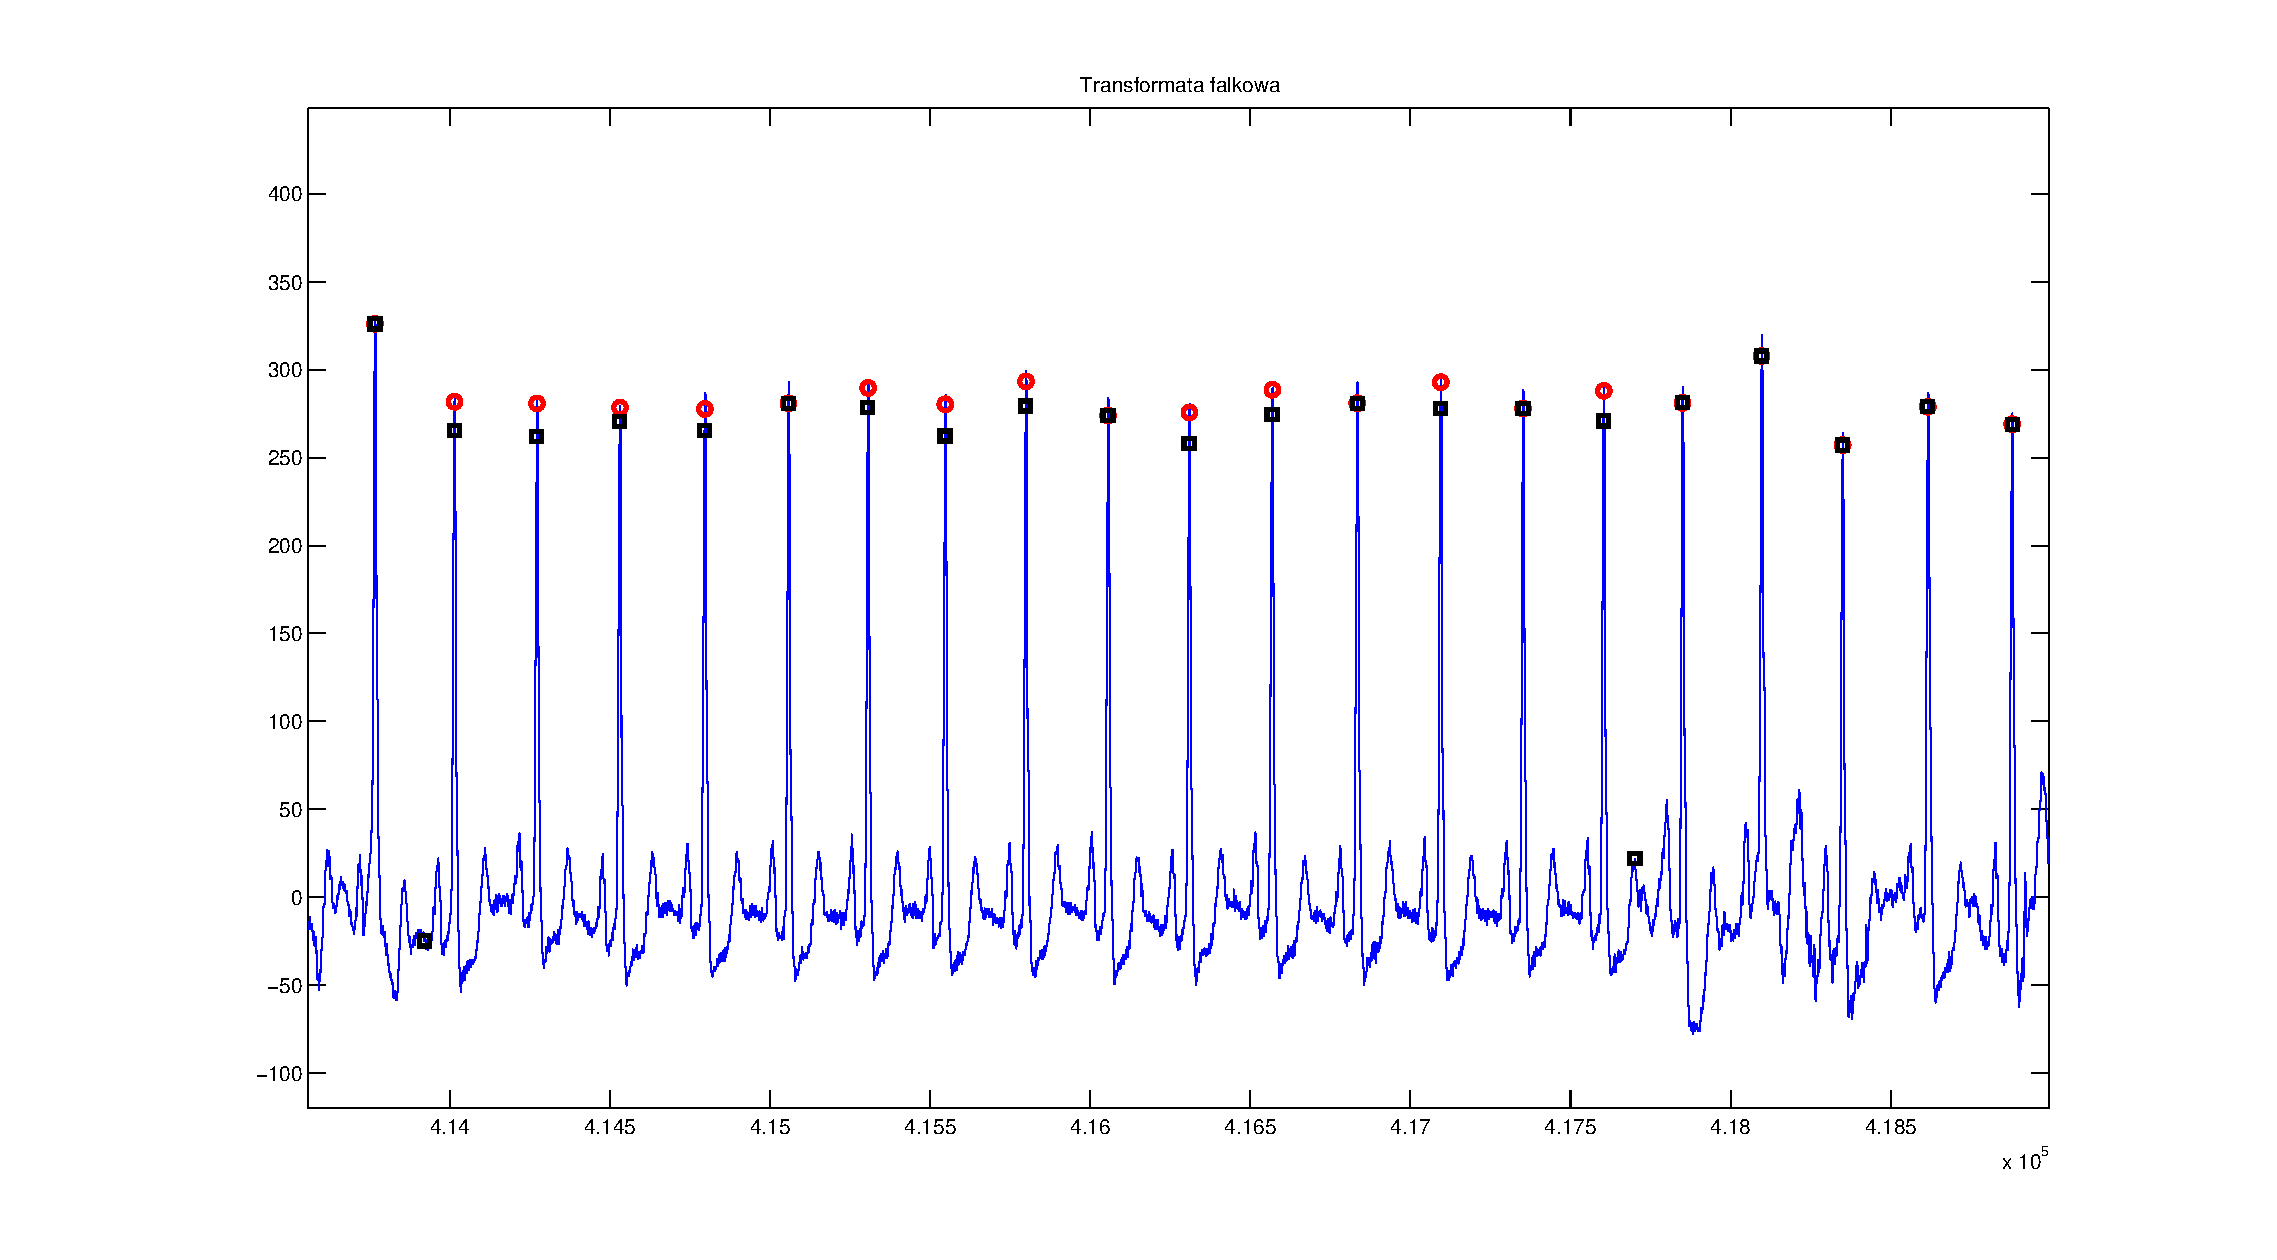
\includegraphics[scale=0.35]{R_PEAKS/wektorowe/105_falka_fragment.eps}
\caption{Fragment sygnału nr 105 - transformata falkowa}
\label{fig:105WF}
\end{figure}
\end{enumerate}
%
%
%
\newpage
\item Sygnał nr 122

Sygnał nr 122 został wybrany ze względu na jego dosyć regularny kształt. Z tego powodu każda z metod bardzo dobrze pozwoliła na detekcje załamków R, co można odnotować czytając dane zawarte w poniższej tabeli.

\begin{table}[H]
\centering
\label{122peaks}
\caption{Załamki R dla sygnału 122}
\begin{tabular}{|l|c|}
\hline
\multicolumn{2}{|c|}{Sygnał nr 122}\\
\hline
Referencyjne & 2479 \\ \hline
Hilbert & 2476 \\ \hline
Pan - Tompkins & 2475 \\ \hline
Transformata falkowa & 2476 \\ \hline
\end{tabular}
\end{table}

\begin{enumerate}[I.]
\item Algorytm bazujący na transformacji Hilberta

Podobnie jak dla sygnału o nr. 105, analiza wykresu \ref{fig:122HC} pozornie może doprowadzić do wniosku, iż różnice między pikami R referencyjnymi oraz wykrytymi na podstawie działania algorytmu bazującego na przekształceniu Hilberta są dosyć znaczne. Wynika to jednak ponownie z faktu, że załamki R są strome i różnica kilku próbek powoduje duże różnice w wartości sygnału, jednak istotą algorytmu detekcji załamków R jest przede wszystkim dostarczenie indeksów próbek.

\newpage
\begin{figure}[H]
\centering
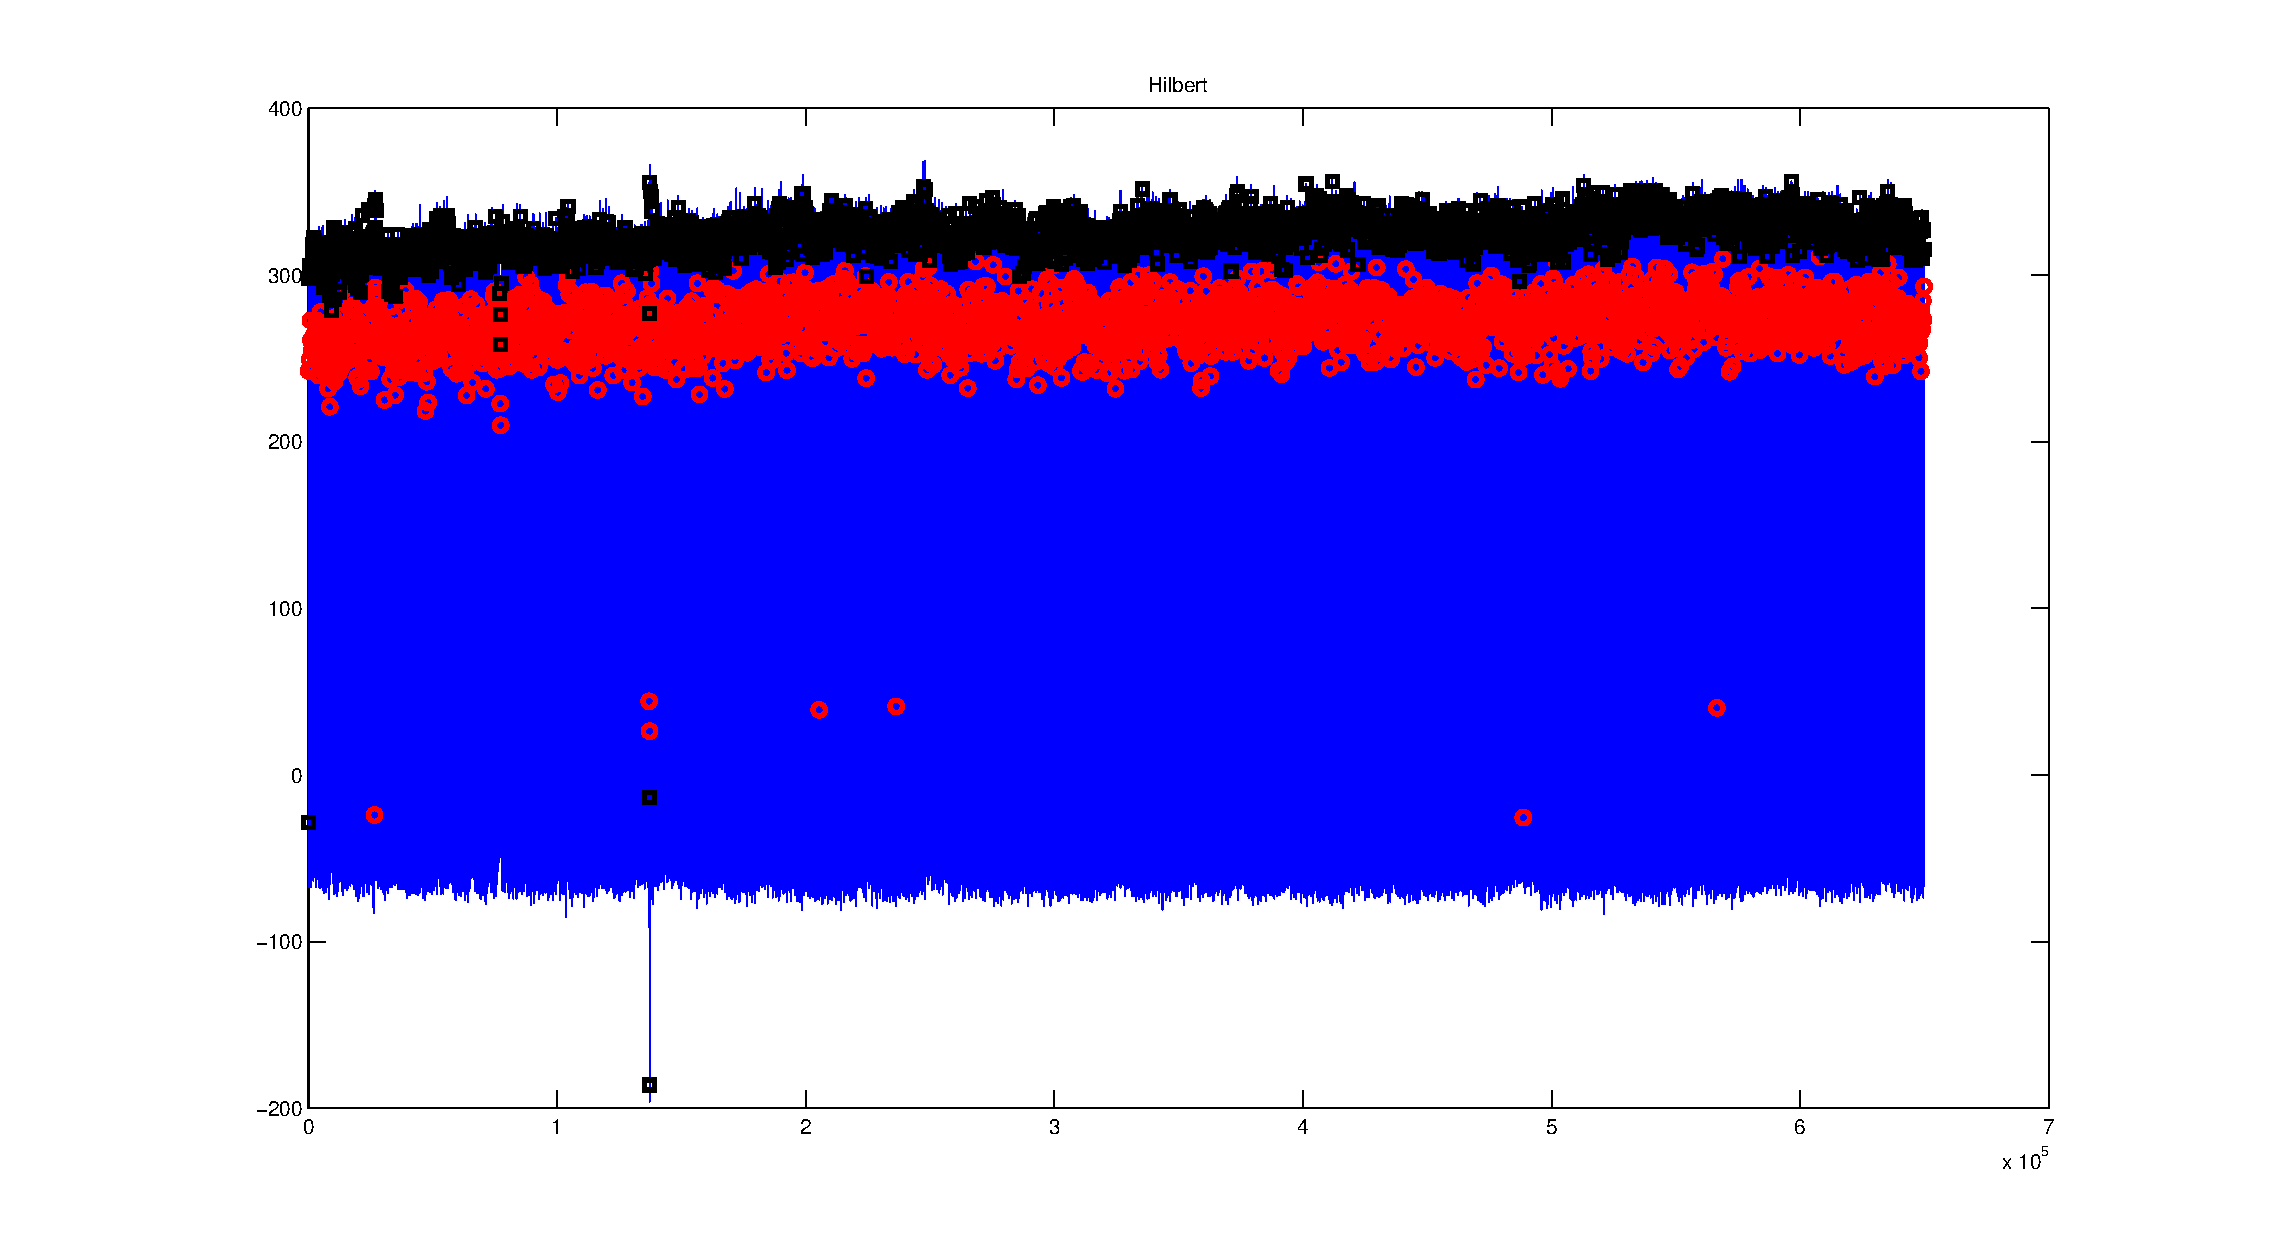
\includegraphics[scale=0.35]{R_PEAKS/wektorowe/122_hilbert_calosc.eps}
\caption{Sygnał nr 122 z naniesionymi pikami R - Hilbert}
\label{fig:122HC}
\end{figure}

\begin{figure}[H]
\centering
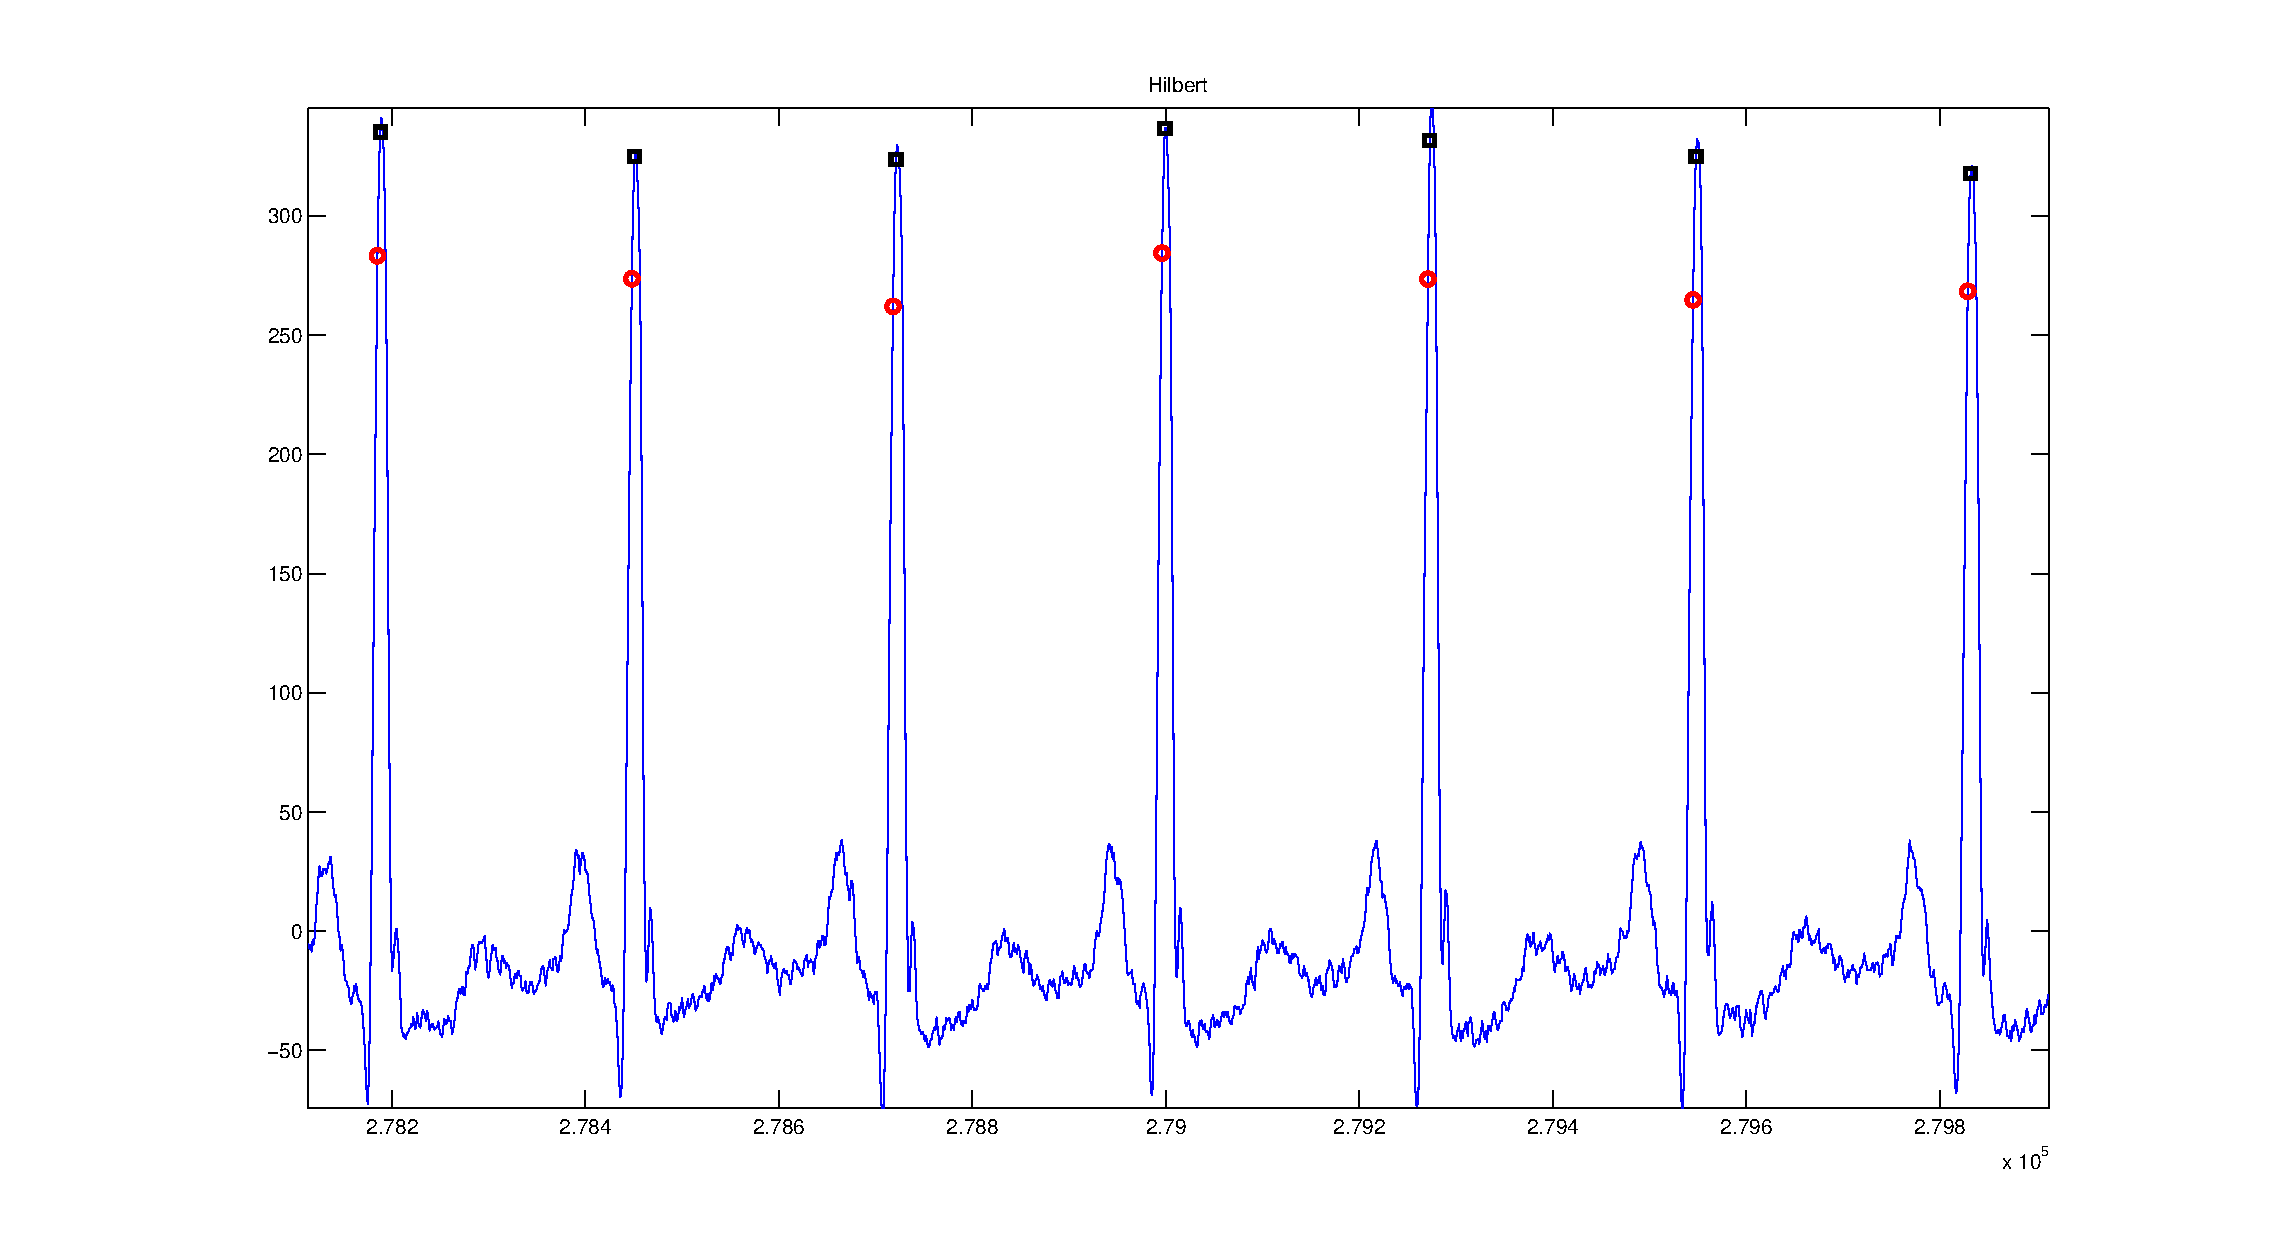
\includegraphics[scale=0.35]{R_PEAKS/wektorowe/122_hilbert_fragment.eps}
\caption{Fragment sygnału nr 122 - Hilbert}
\label{fig:122HF}
\end{figure}
%
%
%
\newpage
\item Algorytm Pan - Tompkins

Na diagramie \ref{fig:122PTC} widać, że różnice pomiędzy załamkami wykrytymi przez algorytm Pan - Tompkins i  referencyjnymi są bardzo małe. Analiza fragmentu sygnału (rys. \ref{fig:122PTF}) tylko to potwierdza. Widać nawet, że niekiedy piki R wykryte przez algorytm są lepsze.

\begin{figure}[H]
\centering
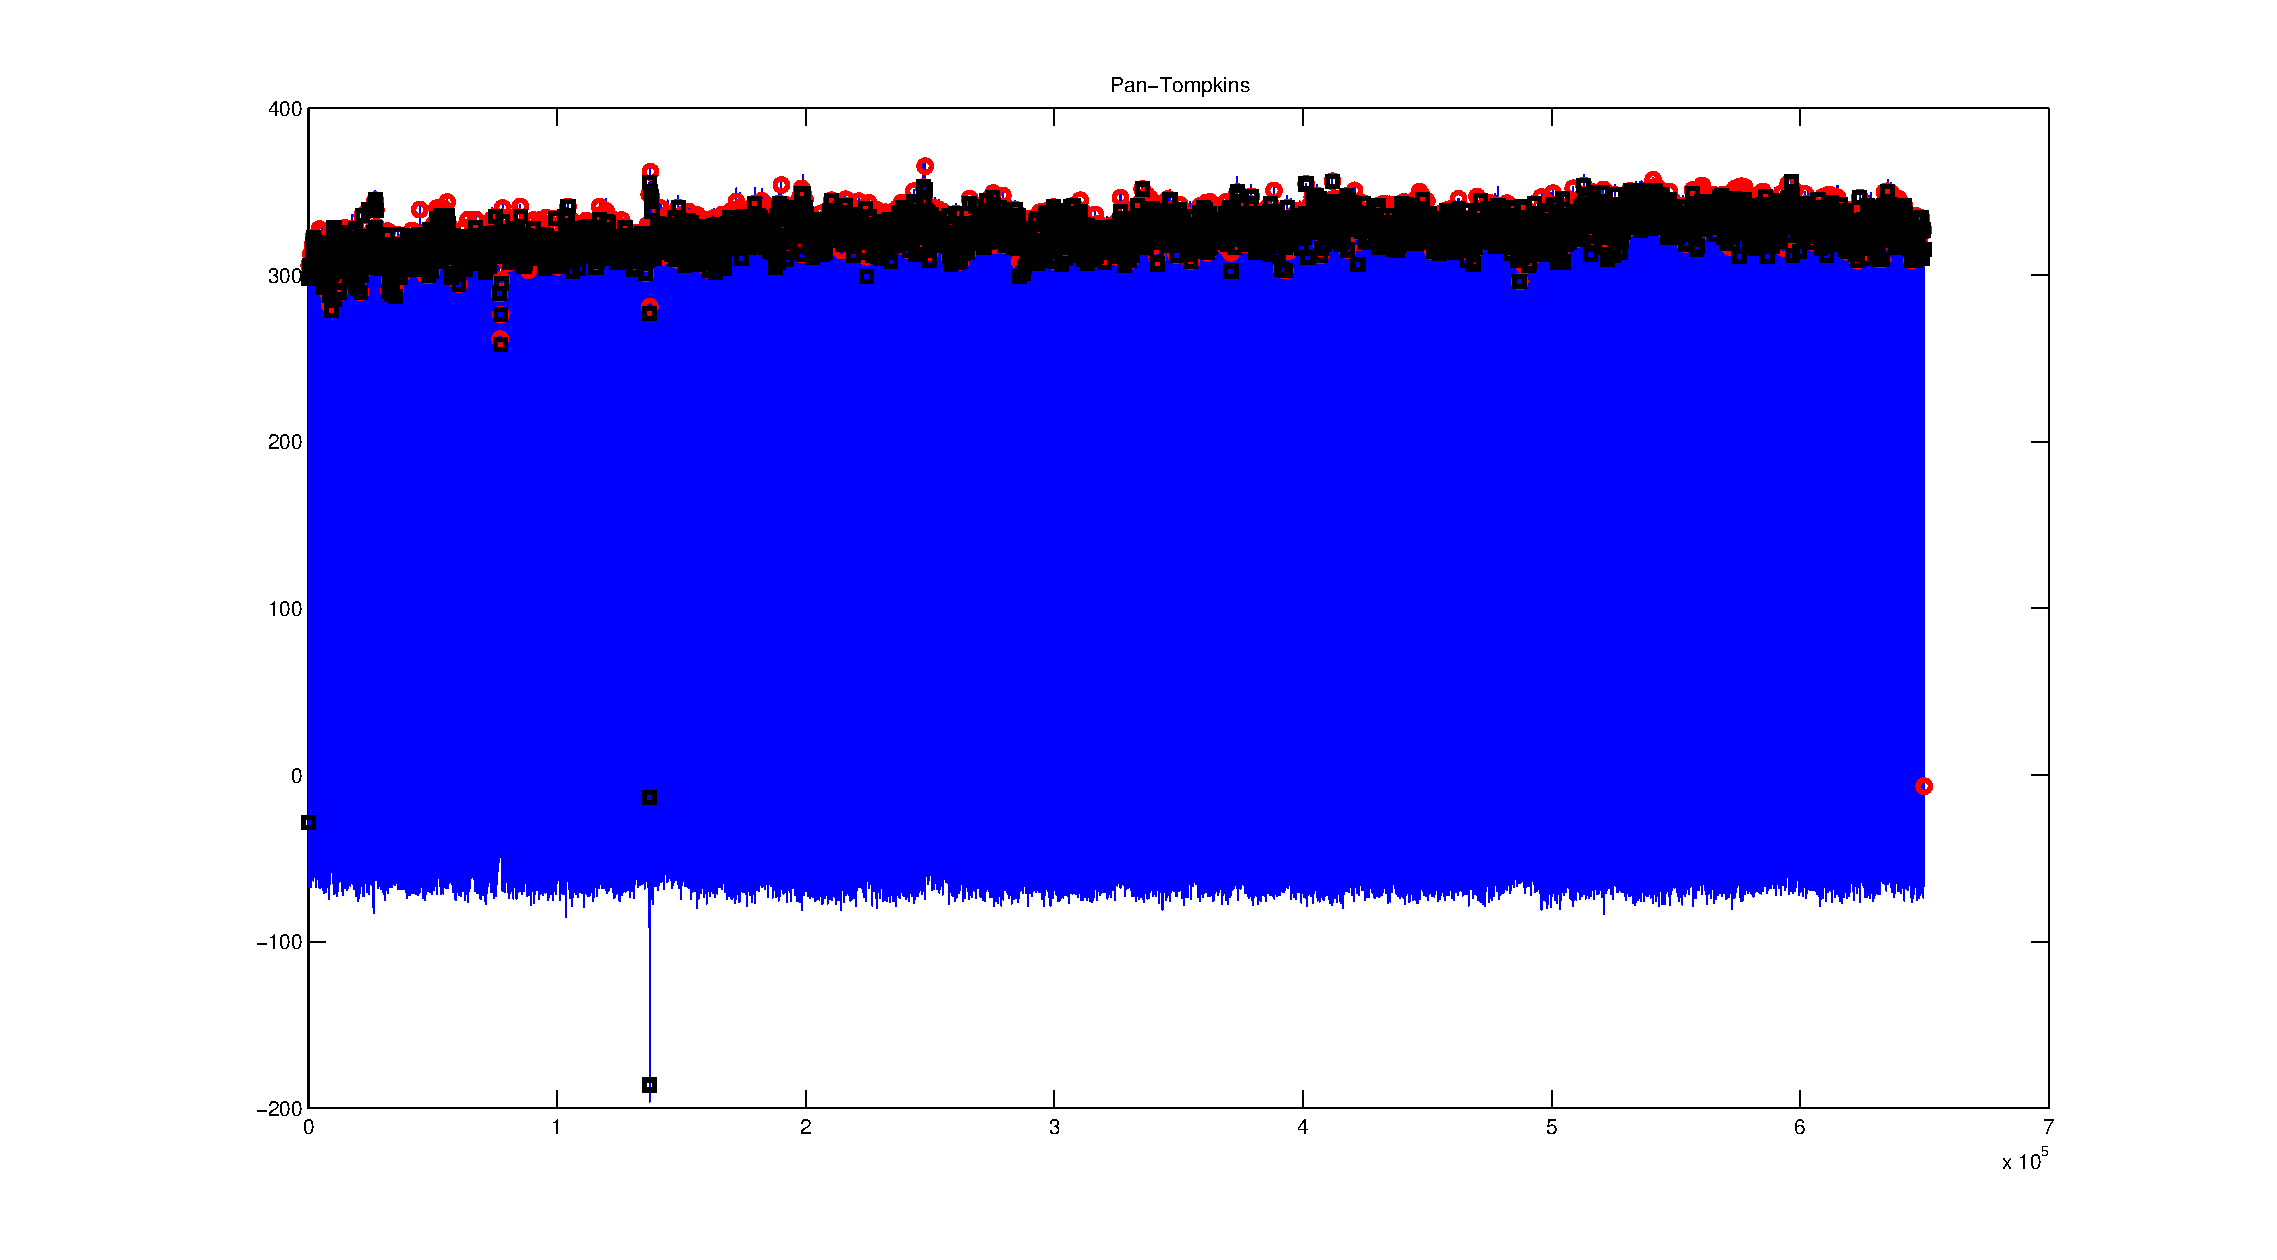
\includegraphics[scale=0.35]{R_PEAKS/wektorowe/122_pan_calosc.eps}
\caption{Sygnał nr 122 z naniesionymi pikami R - Pan - Tompkins}
\label{fig:122PTC}
\end{figure}
\newpage
\begin{figure}[H]
\centering
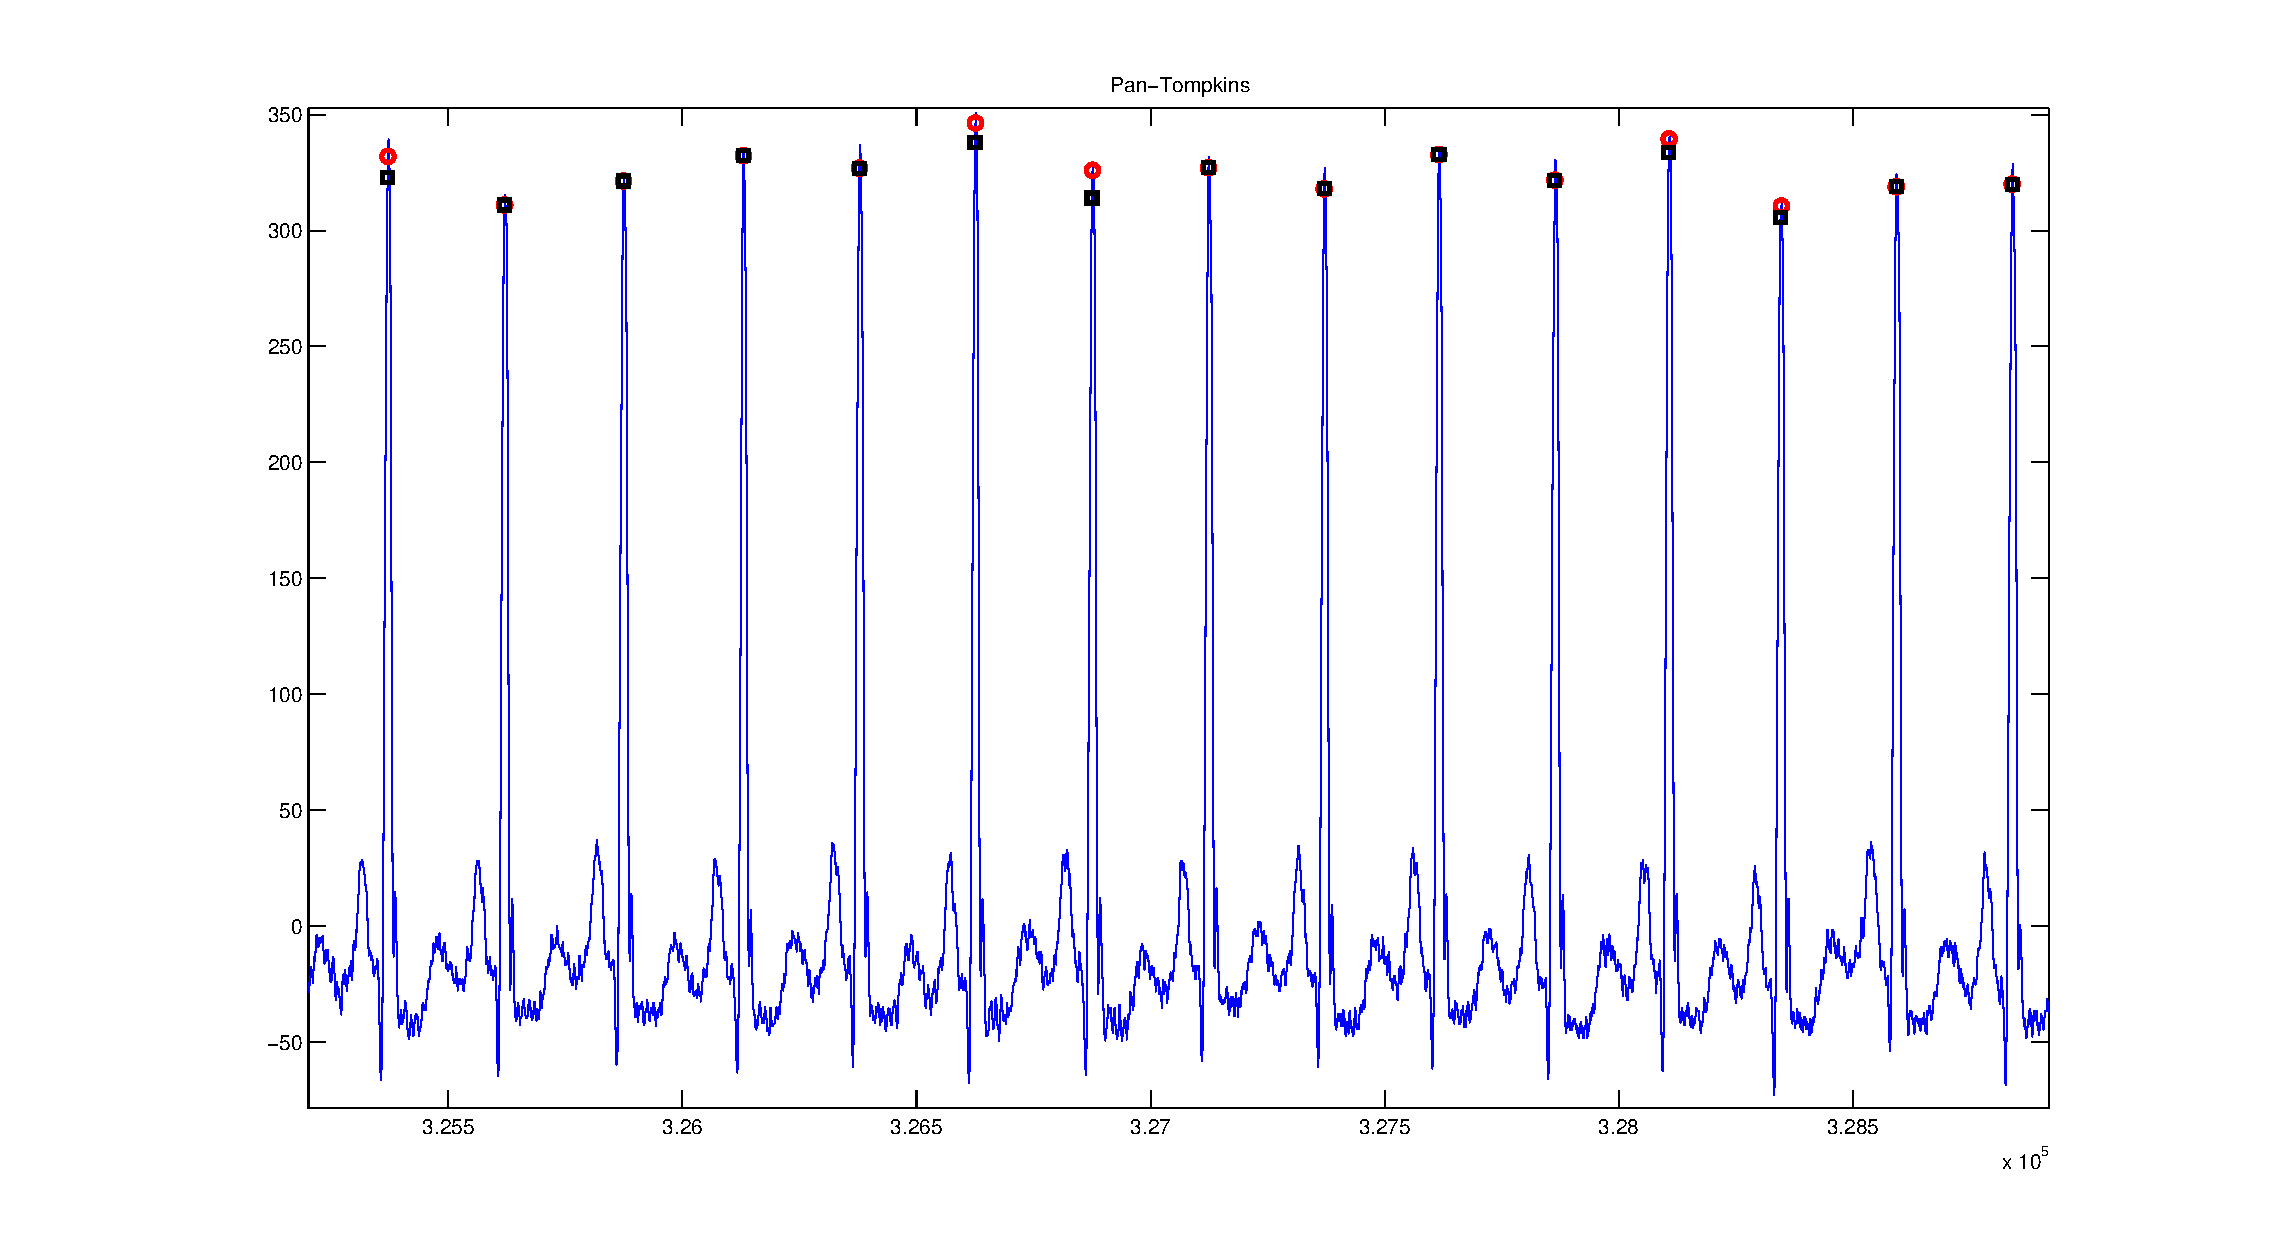
\includegraphics[scale=0.35]{R_PEAKS/wektorowe/122_pan_fragment.eps}
\caption{Fragment sygnału nr 122 - Pan - Tompkins}
\label{fig:122PTF}
\end{figure}
%
%
%
%
\item Algorytm bazujący na transformacji falkowej

Podobnie jak w przypadku algorytmu Pan - Tompkins, algorytm bazujący na transformacji falkowej dostarcza bardzo dobre rezultaty. Wszystkie załamki są o podobnej amplitudzie, więc algorytm nie wprowadza przekłamań. Na fragmencie sygnału (rys. \ref{fig:122WF}) widać, że załamki wykryte przez algorytm pokrywają się z załamkami referencyjnymi, lub są nawet lepsze.
\newpage
\begin{figure}[H]
\centering
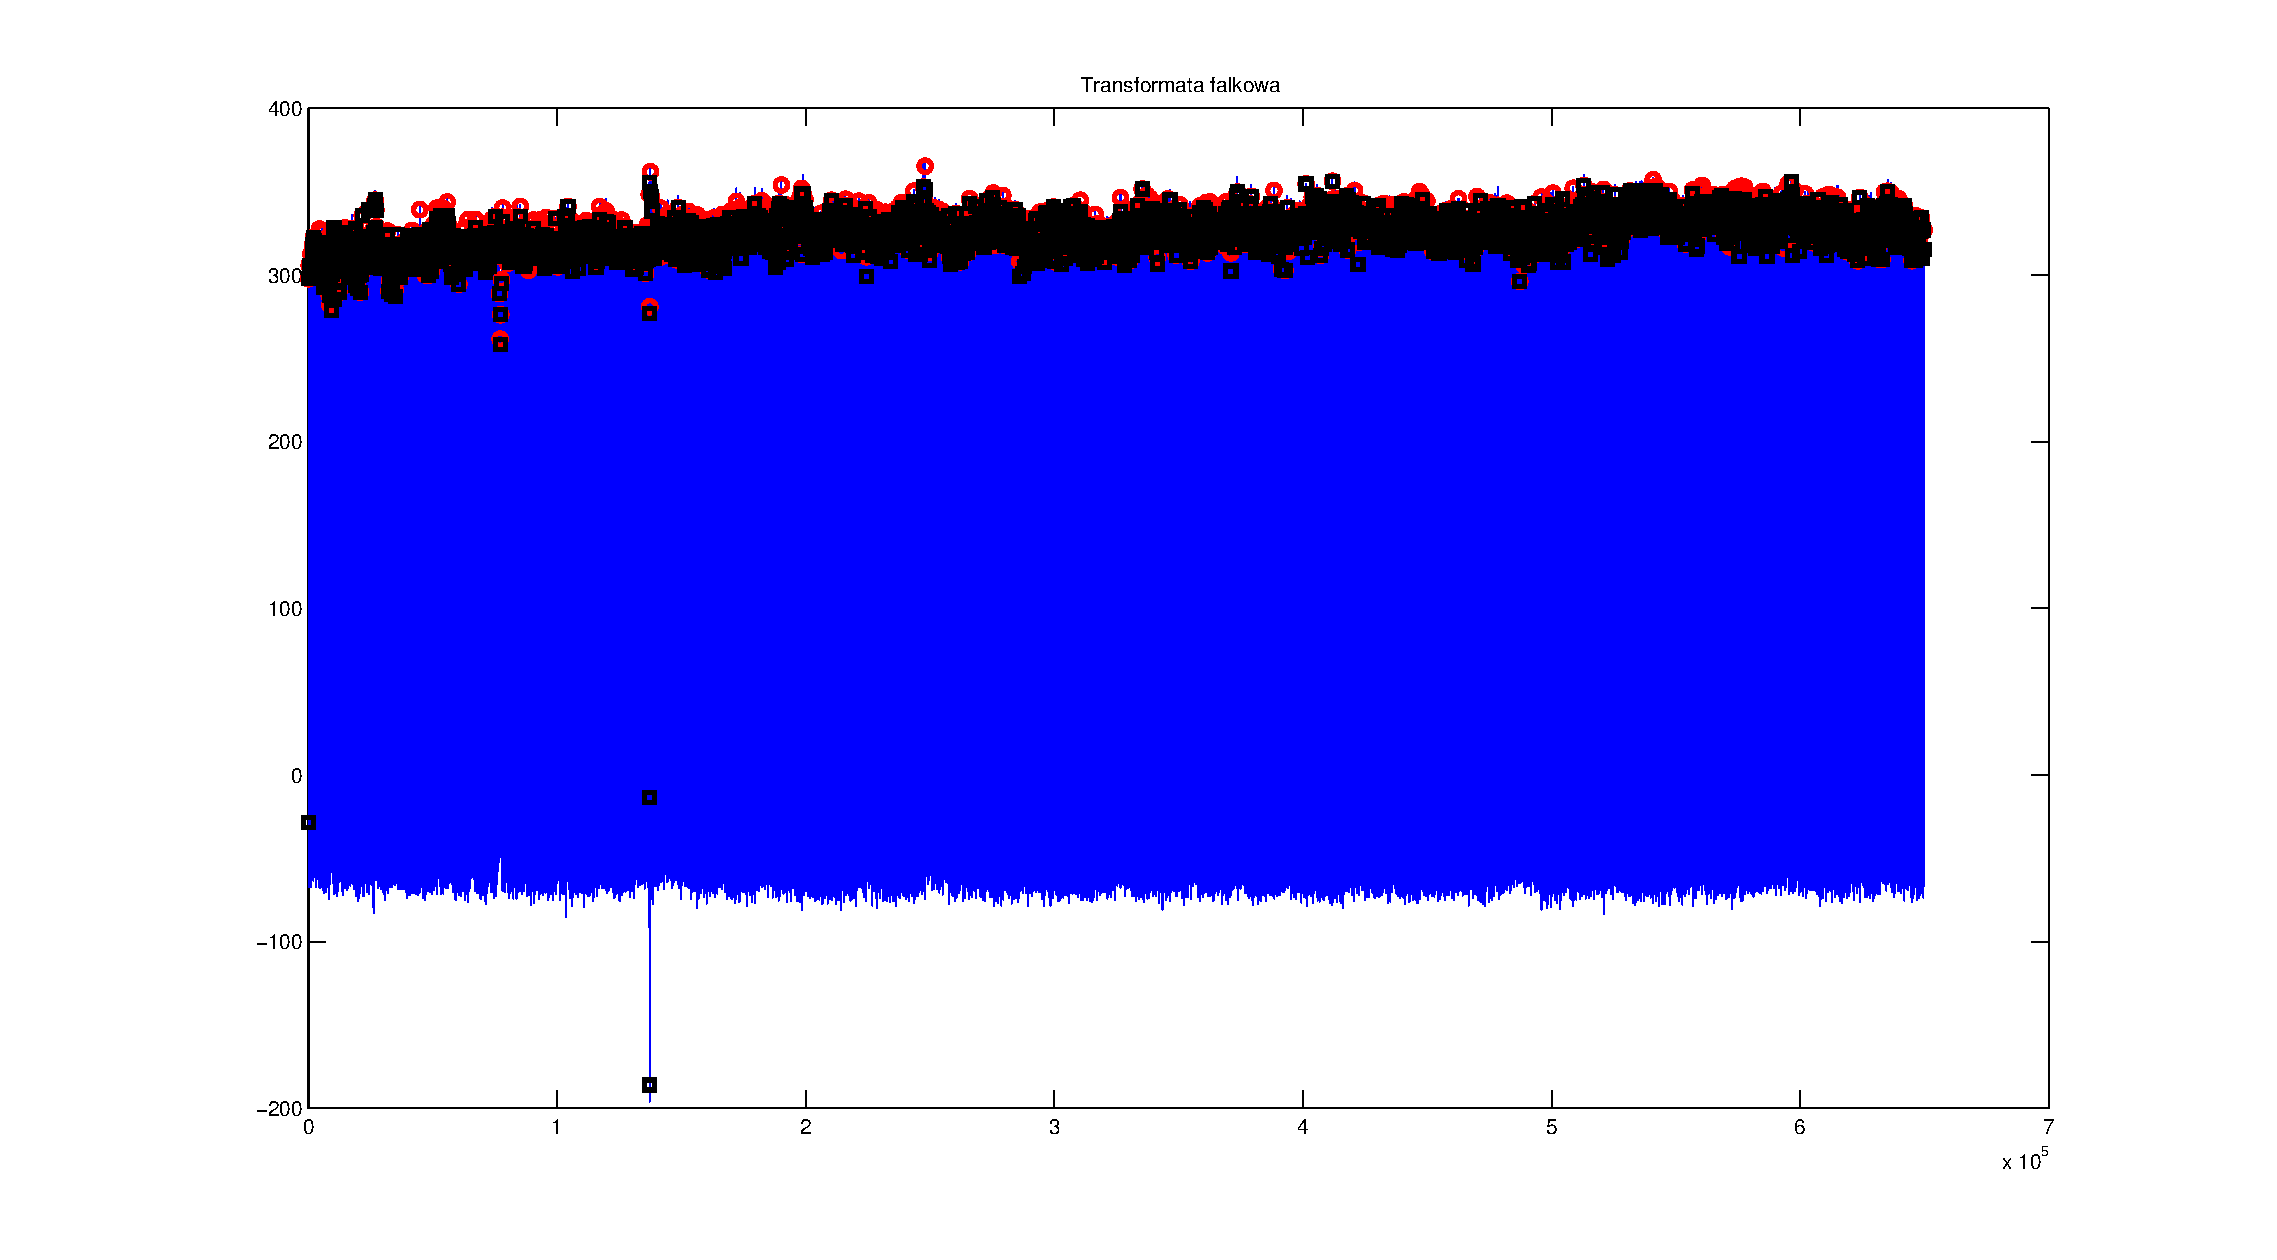
\includegraphics[scale=0.35]{R_PEAKS/wektorowe/122_falka_calosc.eps}
\caption{Sygnał nr 122 z naniesionymi pikami R - transformata falkowa}
\label{fig:122WC}
\end{figure}

\begin{figure}[H]
\centering
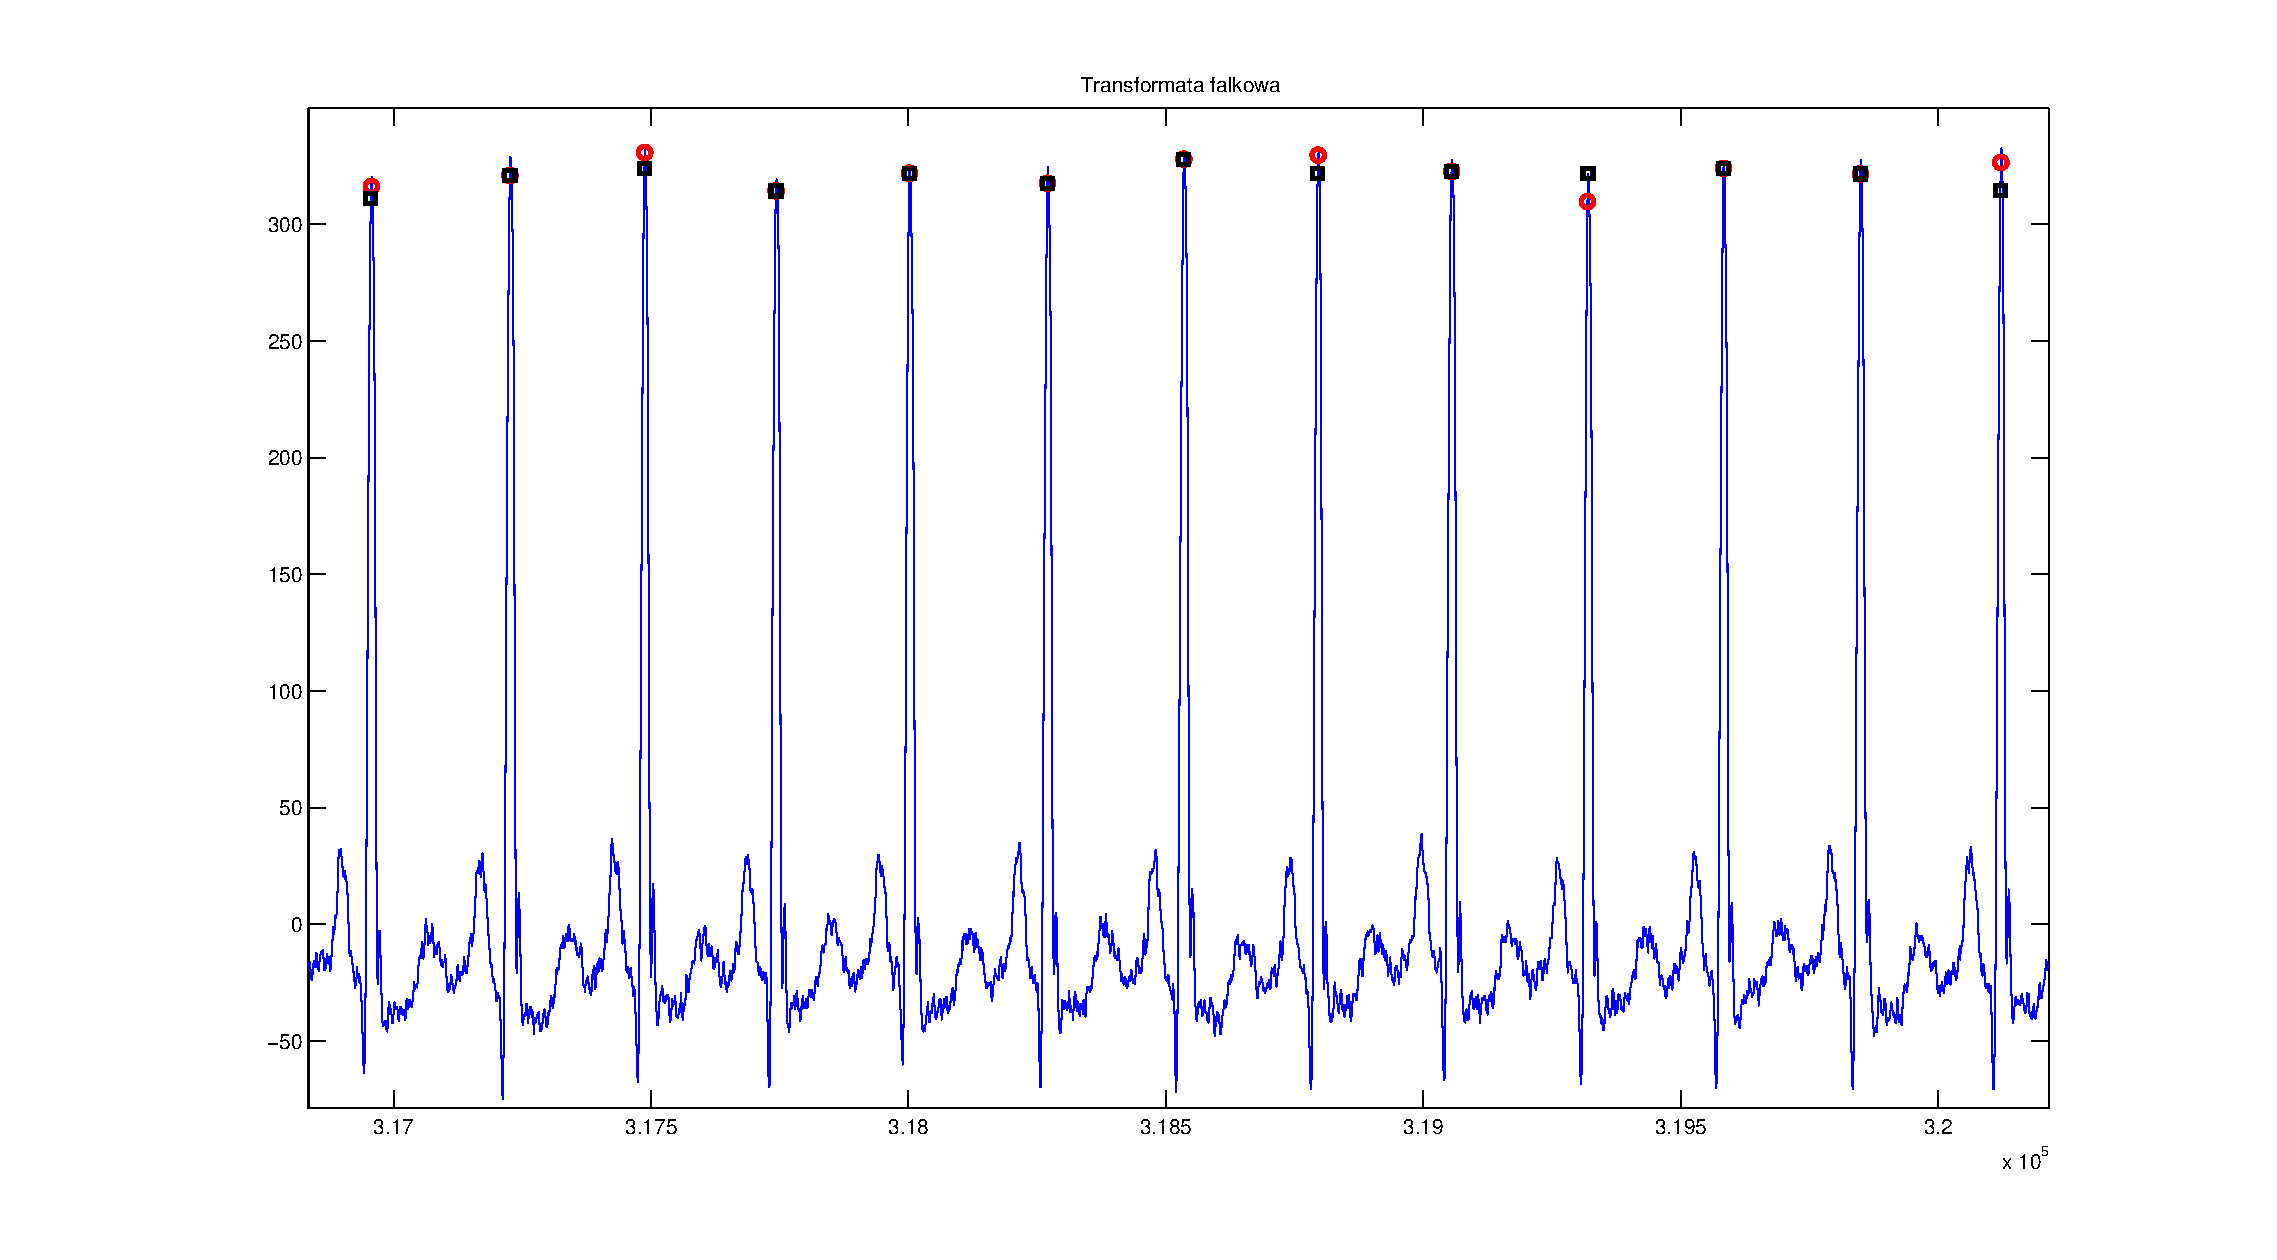
\includegraphics[scale=0.35]{R_PEAKS/wektorowe/122_falka_fragment.eps}
\caption{Fragment sygnału nr 122 - transformata falkowa}
\label{fig:122WF}
\end{figure}
\end{enumerate}
%
%
%
\newpage
\item Sygnał nr 228

Sygnał nr 228 został wybrany ze względu na jego ciekawy, nieregularny kształt. Z tego powodu algorytm bazujący na transformacie falkowej kompletnie zawiódł - wykryto jedynie ok. 25\% wszystkim załamków.

\begin{table}[H]
\centering
\label{228peaks}
\caption{Załamki R dla sygnału 228}
\begin{tabular}{|l|c|}
\hline
\multicolumn{2}{|c|}{Sygnał nr 228}\\
\hline
Referencyjne & 2141 \\ \hline
Hilbert & 2094 \\ \hline
Pan - Tompkins & 1890 \\ \hline
Transformata falkowa & 568 \\ \hline
\end{tabular}
\end{table}

\begin{enumerate}[I.]
\item Algorytm bazujący na transformacji Hilberta

Analizując wykres całego przebiegu sygnału (rys. \ref{fig:228HC}) można dojść do wniosku, że algorytm bazujący na transformacie Hilberta dosyć dobrze wywiązał się z zadania, aczkolwiek różnice są widoczne. Na fragmencie sygnału (rys. \ref{fig:228HF} widać, że w przypadku wykrytych w miarę poprawnie załamków, różnice są rzędu kilku próbek, natomiast widać, również piki, które nie zostały w ogóle wykryte, lub nawet pewne nadmiarowe załamki. Ostatni przypadek oznacza jednak, że w przekroju całego sygnału dużo załamków musiało być pominiętych - liczba wszystkich wykrytych załamków jest mniejsza od liczby pików referencyjnych. 

\newpage
\begin{figure}[H]
\centering
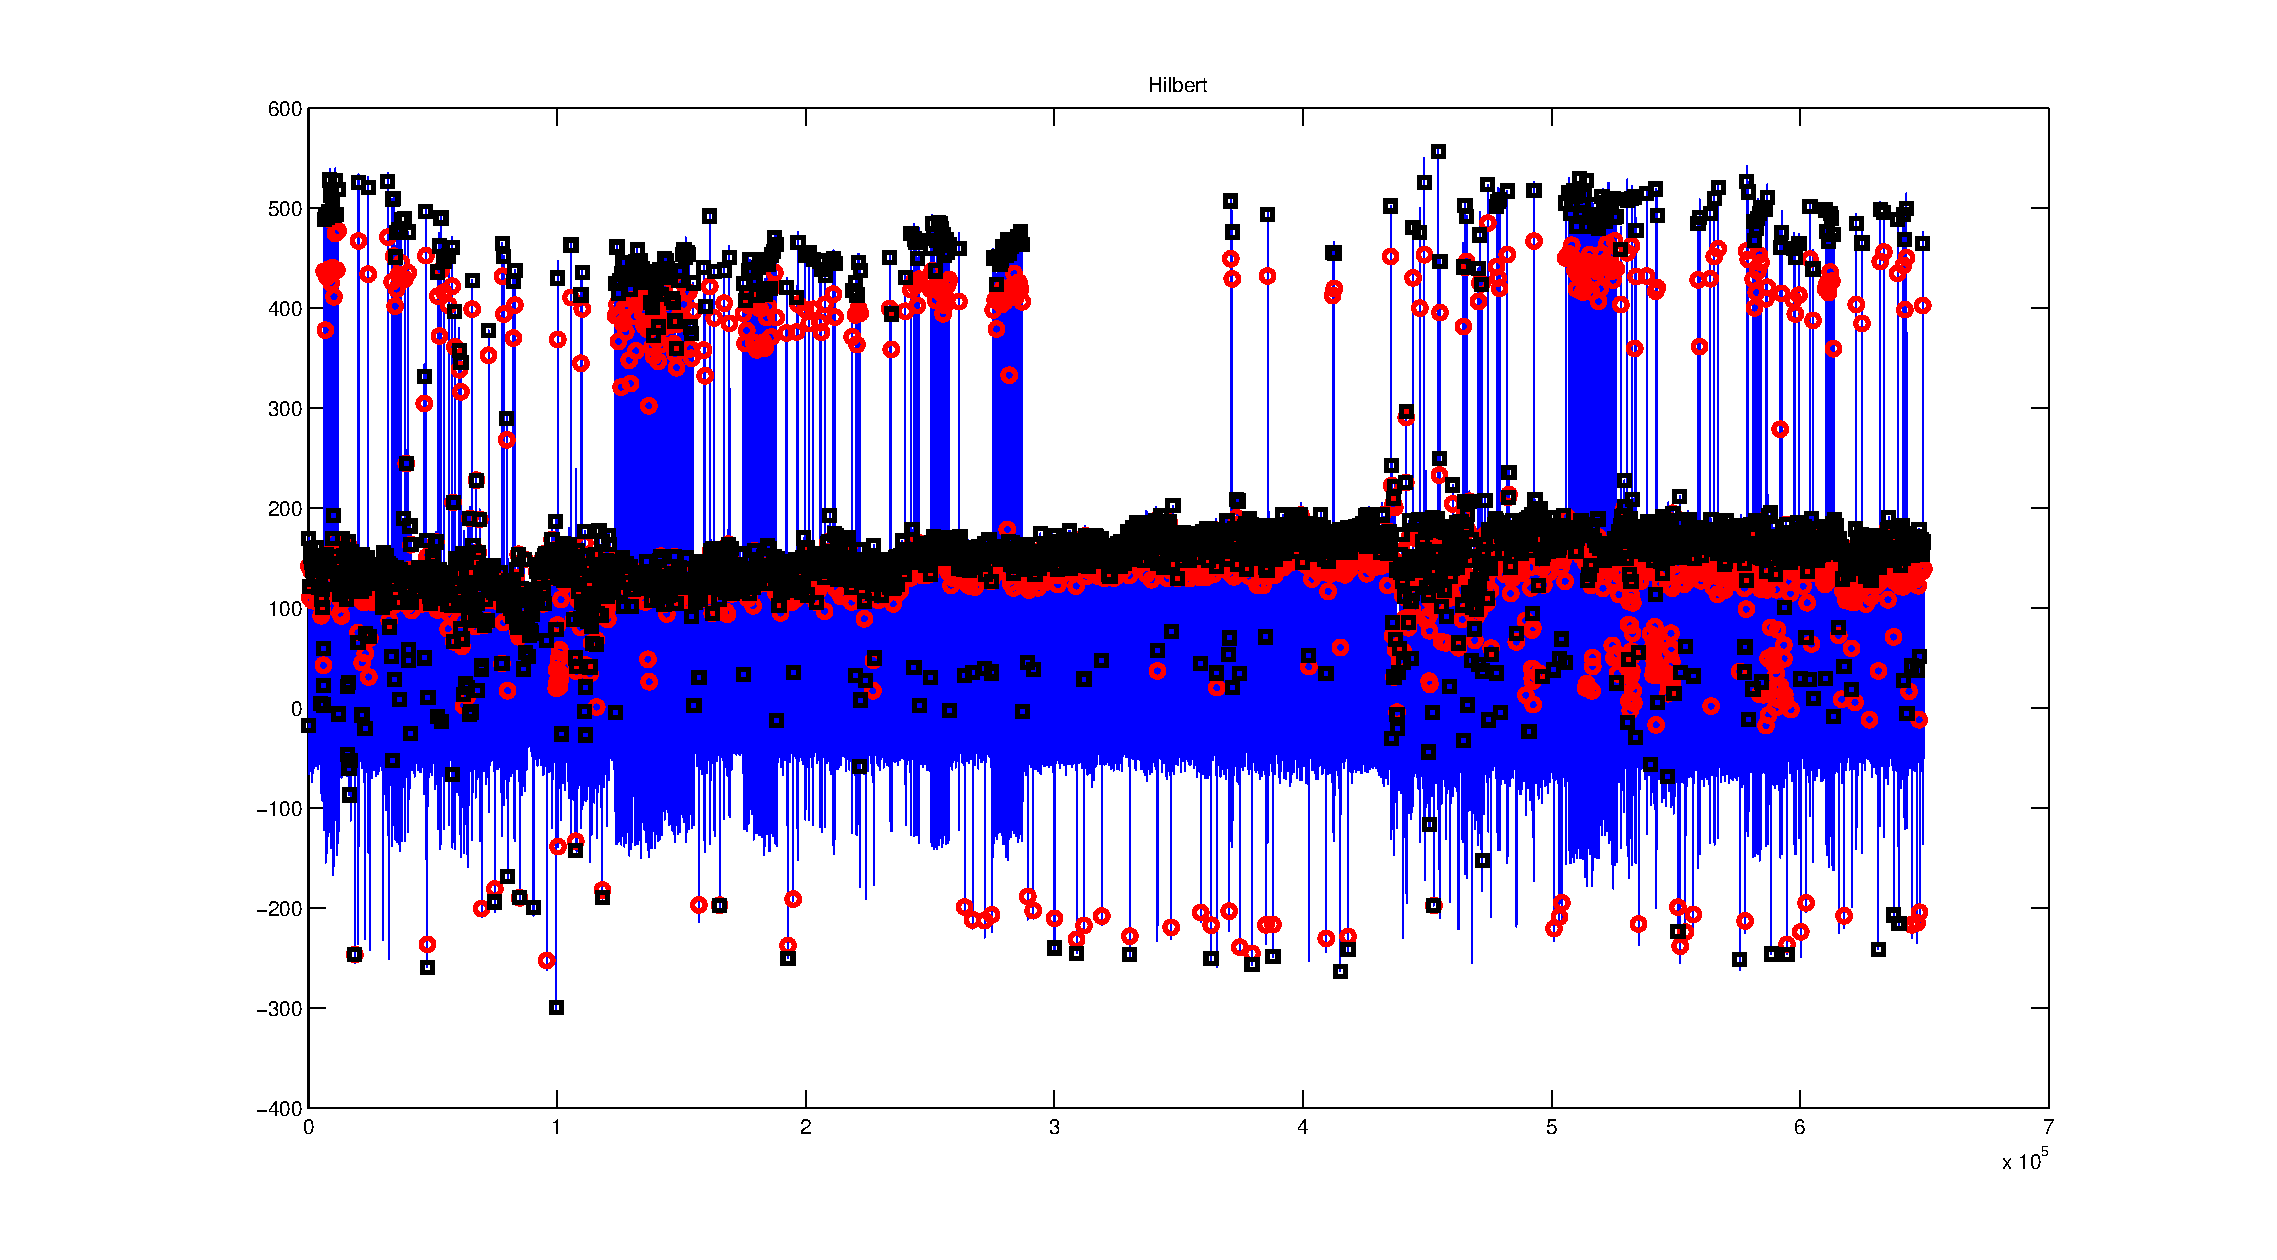
\includegraphics[scale=0.35]{R_PEAKS/wektorowe/228_hilbert_calosc.eps}
\caption{Sygnał nr 228 z naniesionymi pikami R - Hilbert}
\label{fig:228HC}
\end{figure}

\begin{figure}[H]
\centering
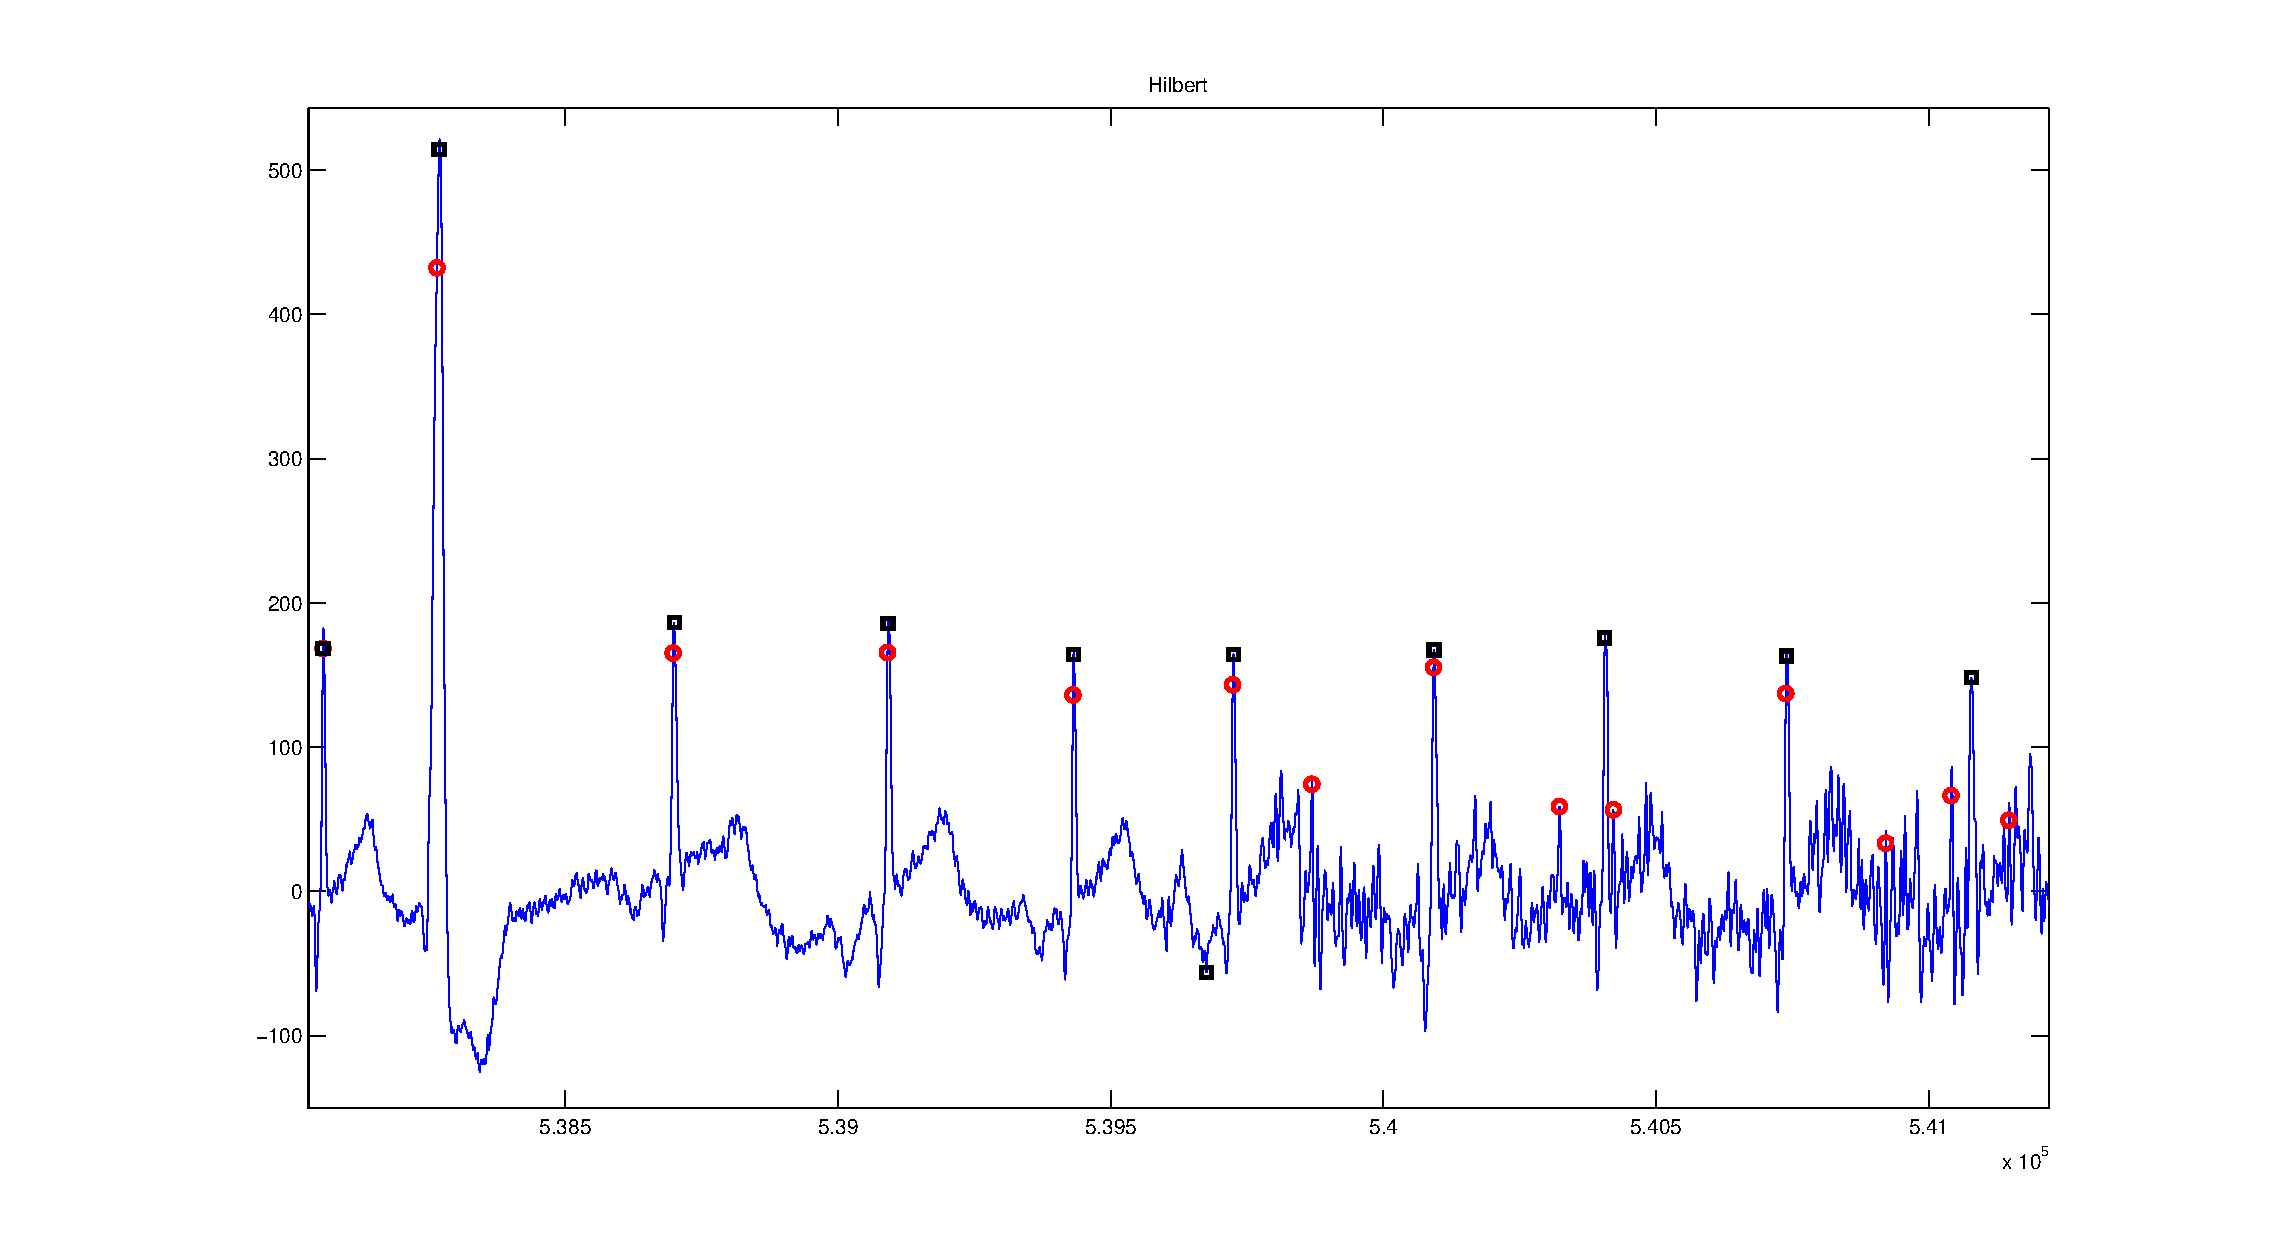
\includegraphics[scale=0.35]{R_PEAKS/wektorowe/228_hilbert_fragment.eps}
\caption{Fragment sygnału nr 228 - Hilbert}
\label{fig:228HF}
\end{figure}
%
%
%
\newpage
\item Algorytm Pan - Tompkins

Na wykresie \ref{fig:228PTC} widać, że wykryto większość załamków i różnice między nimi i referencyjnymi są małe. Analiza fragmentu sygnału tylko to potwierdza - piki wykryte przez algorytm Pan - Tompkins pokrywają się z referencyjnymi, a nieraz nawet są lepsze.

\begin{figure}[H]
\centering
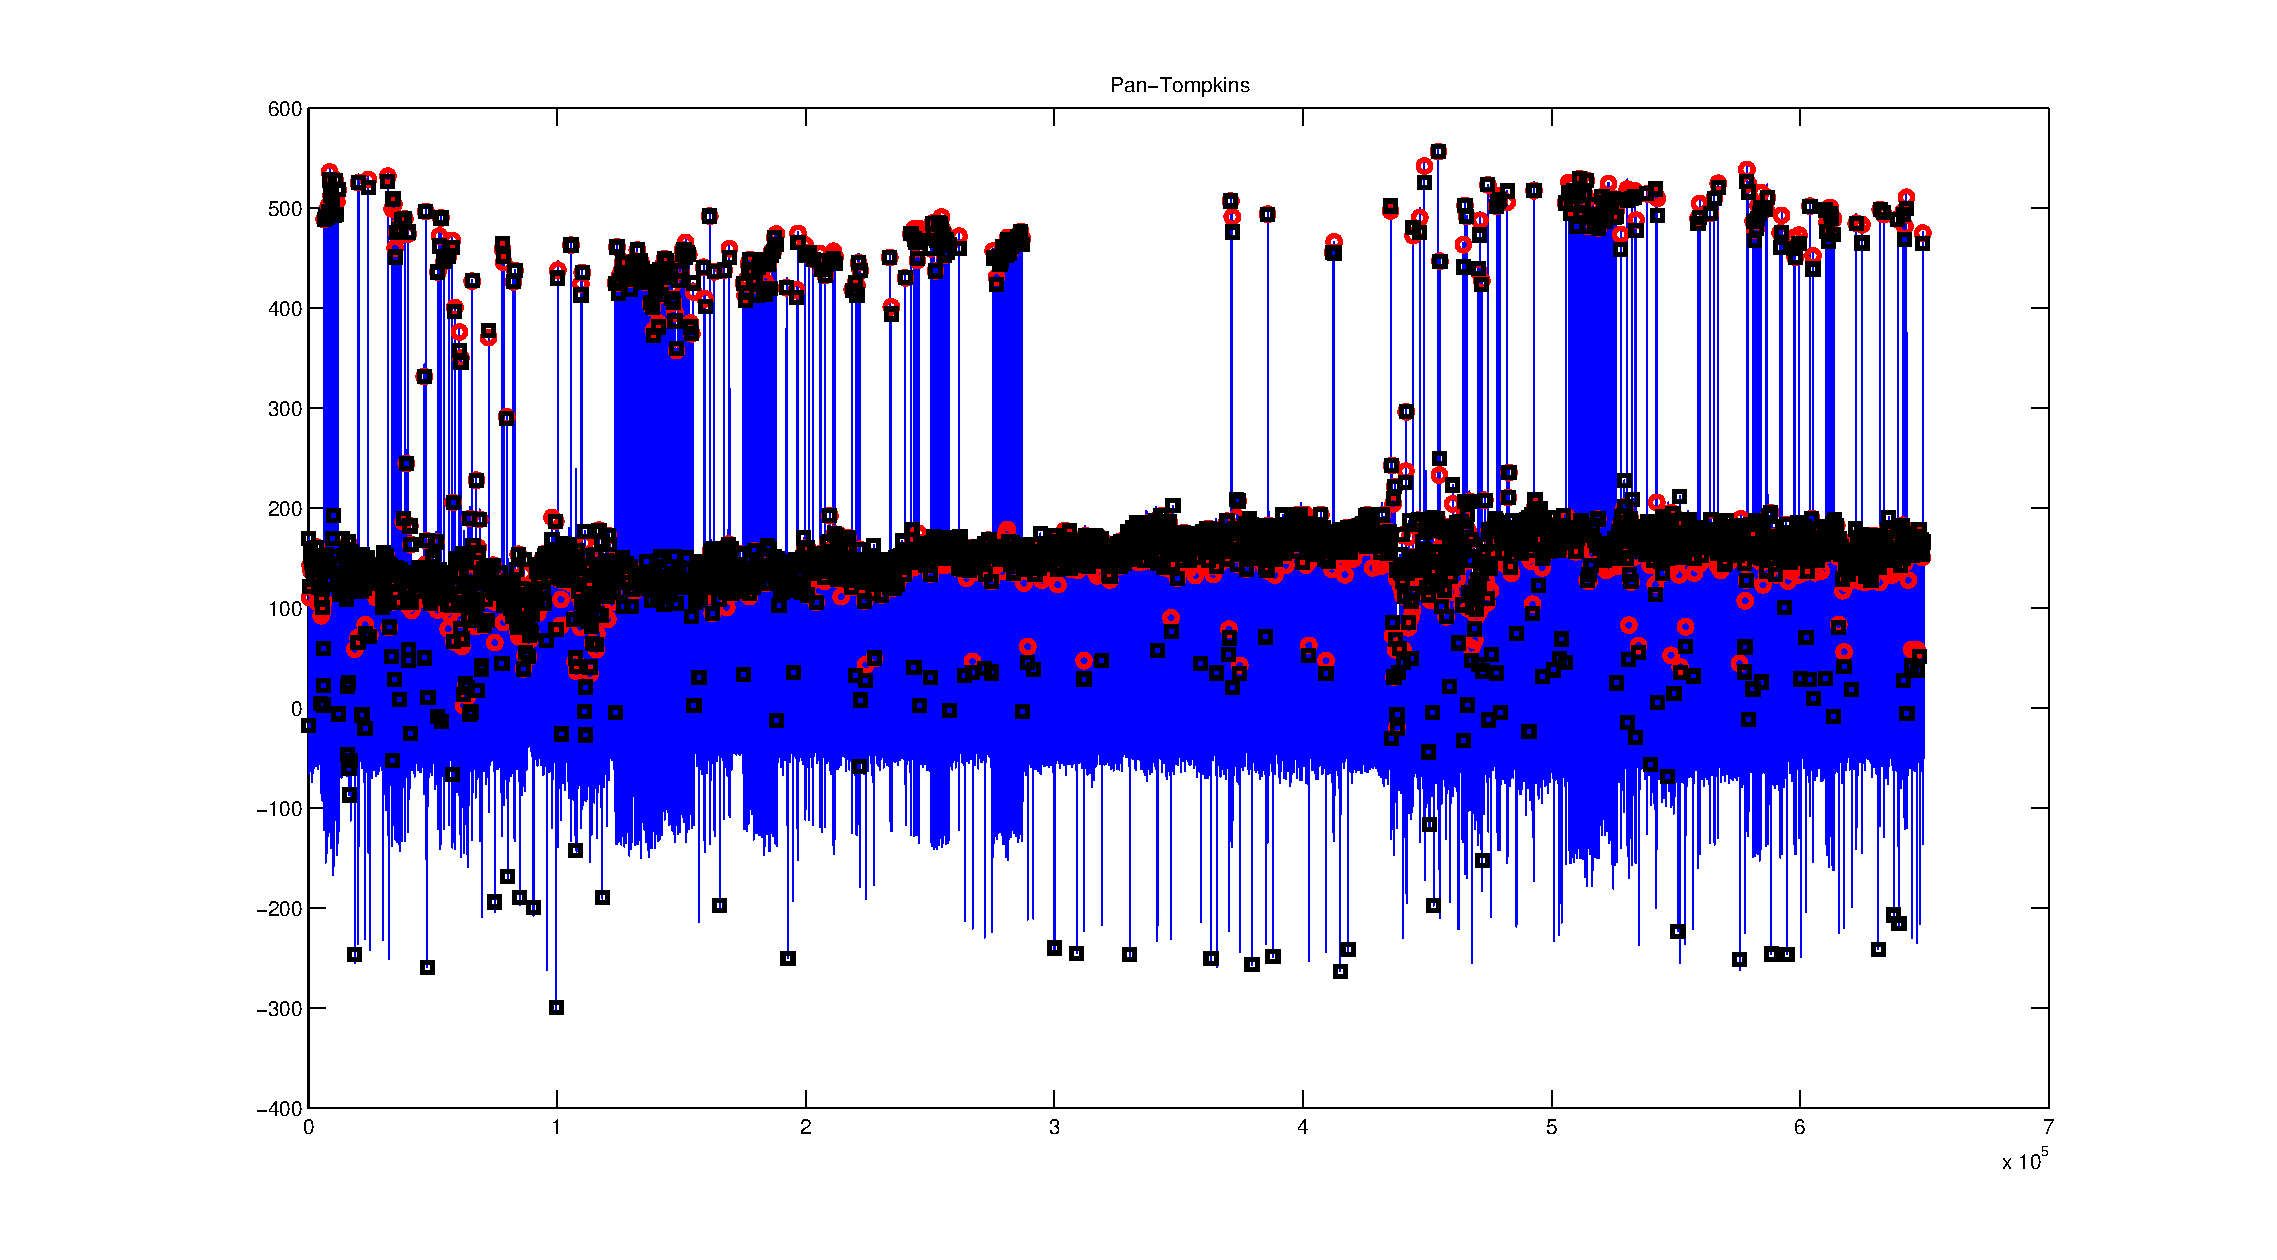
\includegraphics[scale=0.35]{R_PEAKS/wektorowe/228_pan_calosc.eps}
\caption{Sygnał nr 228 z naniesionymi pikami R - Pan - Tompkins}
\label{fig:228PTC}
\end{figure}
\newpage
\begin{figure}[H]
\centering
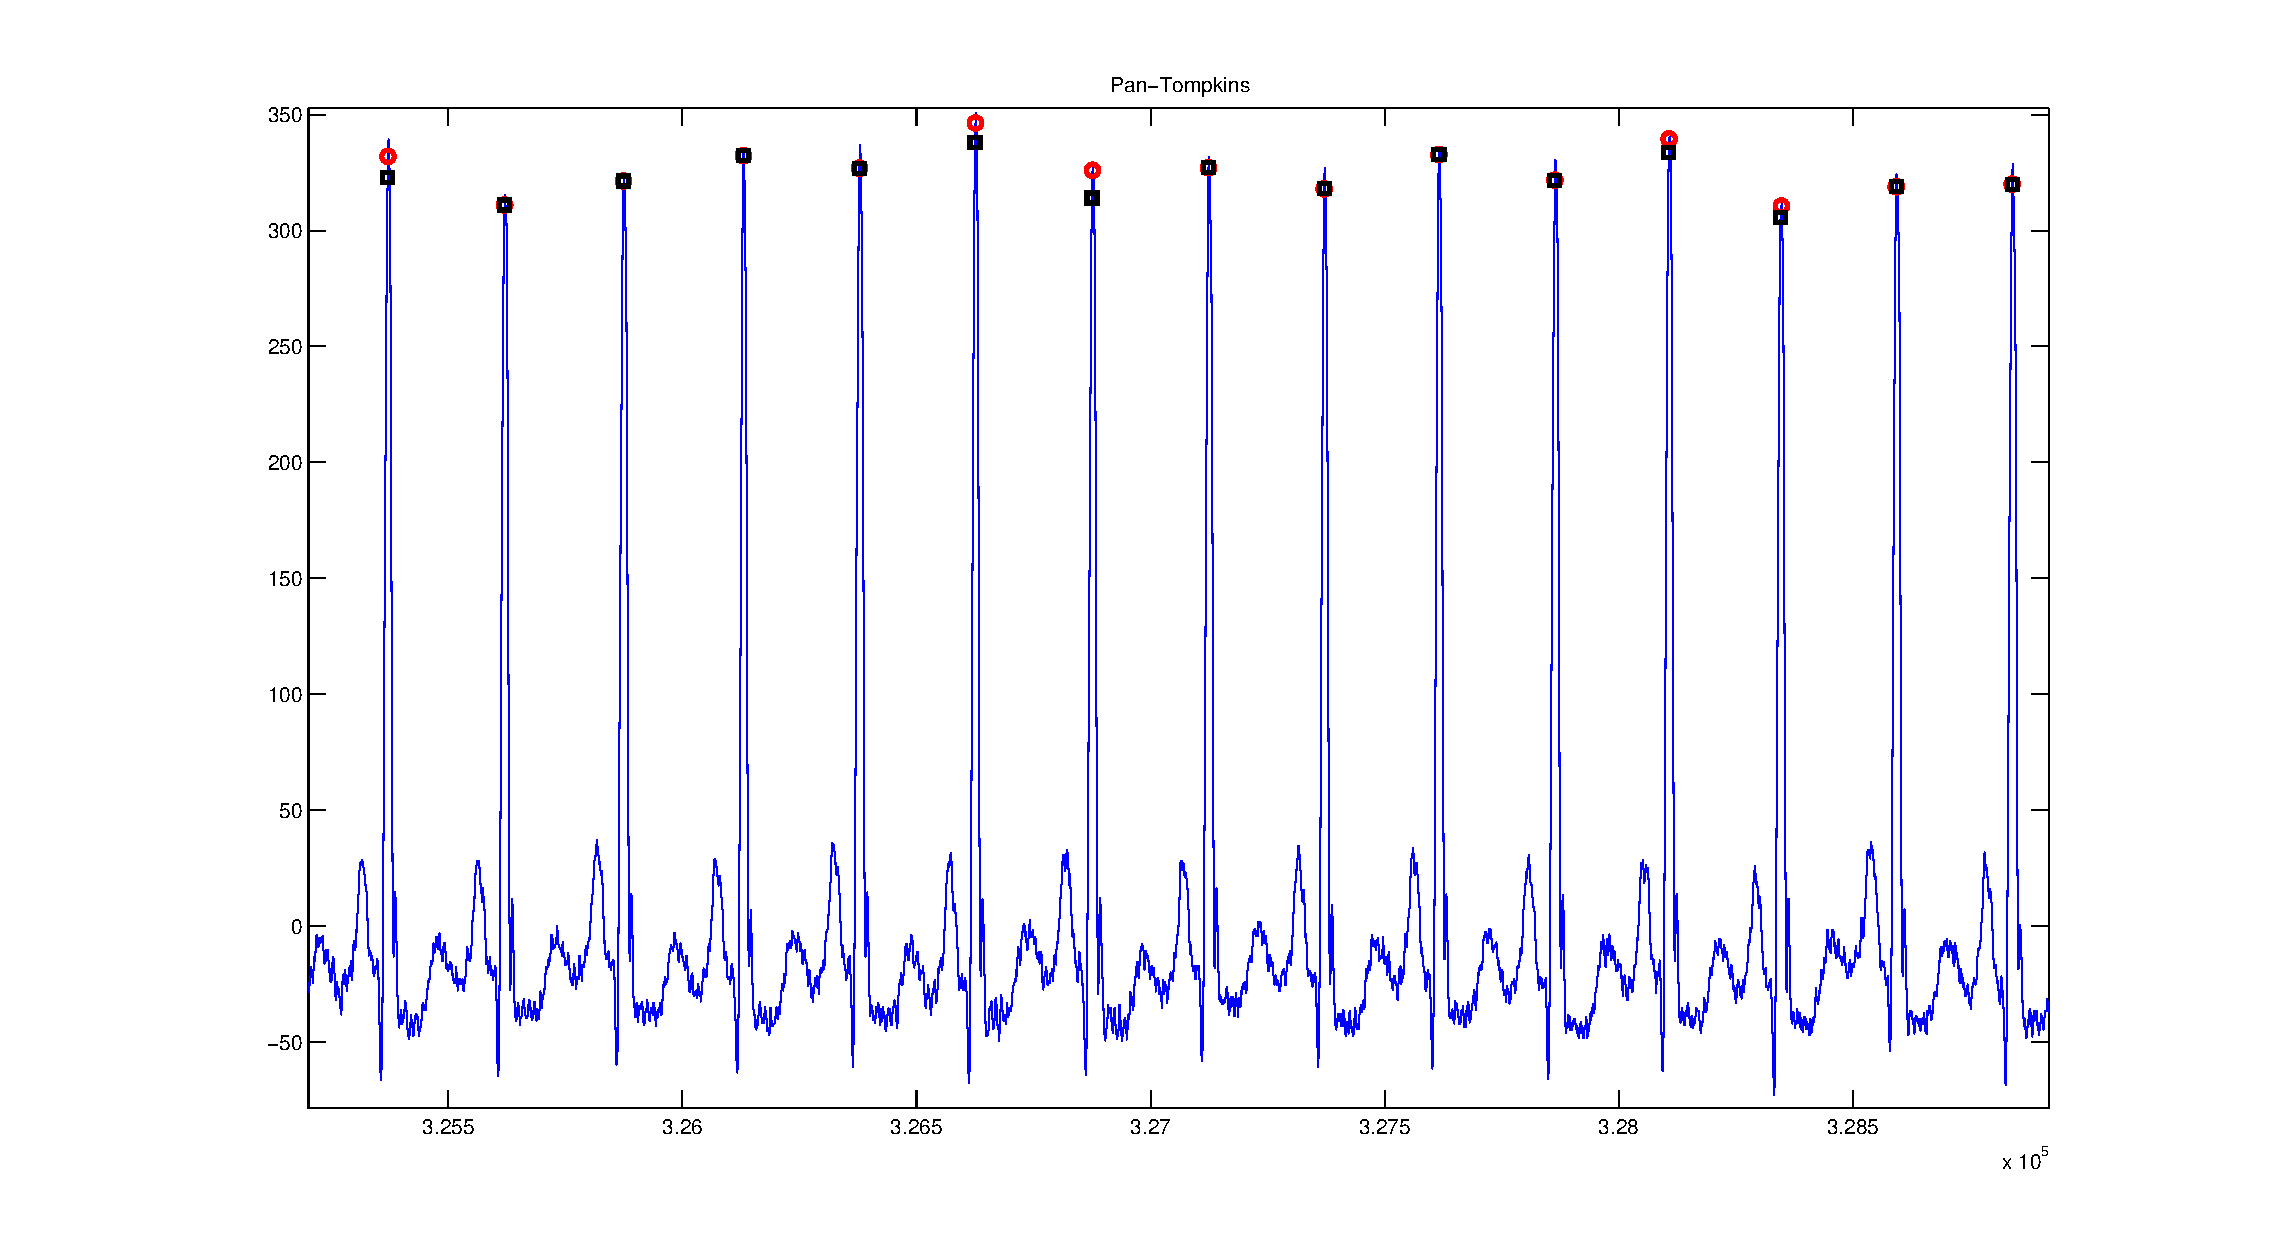
\includegraphics[scale=0.35]{R_PEAKS/wektorowe/122_pan_fragment.eps}
\caption{Fragment sygnału nr 228 - Pan - Tompkins}
\label{fig:228PTF}
\end{figure}
%
%
%
%
\item Algorytm bazujący na transformacji falkowej

Sygnał nr 228 jest dobrym przykładem sygnału, dla którego algorytm opierający swoje działanie na transformacie falkowej nie radzi sobie. Z powodu, iż różnice w amplitudzie sygnału dla niektórych załamków R są znaczne, algorytm może nie wykryć pików o małej wartości. Wprawdzie w przypadku wykrytych załamków rezultaty są dobre, to w kontekście całego sygnału wyniki są słabe. Dobrze widoczne jest to na fragmencie sygnału (rys. \ref{fig:228WF}). Widać bardzo dużo niskich załamków, które zostały pominięte przez algorytm. Piki o dużej amplitudzie zostały wykryte bardzo dobrze.
\newpage
\begin{figure}[H]
\centering
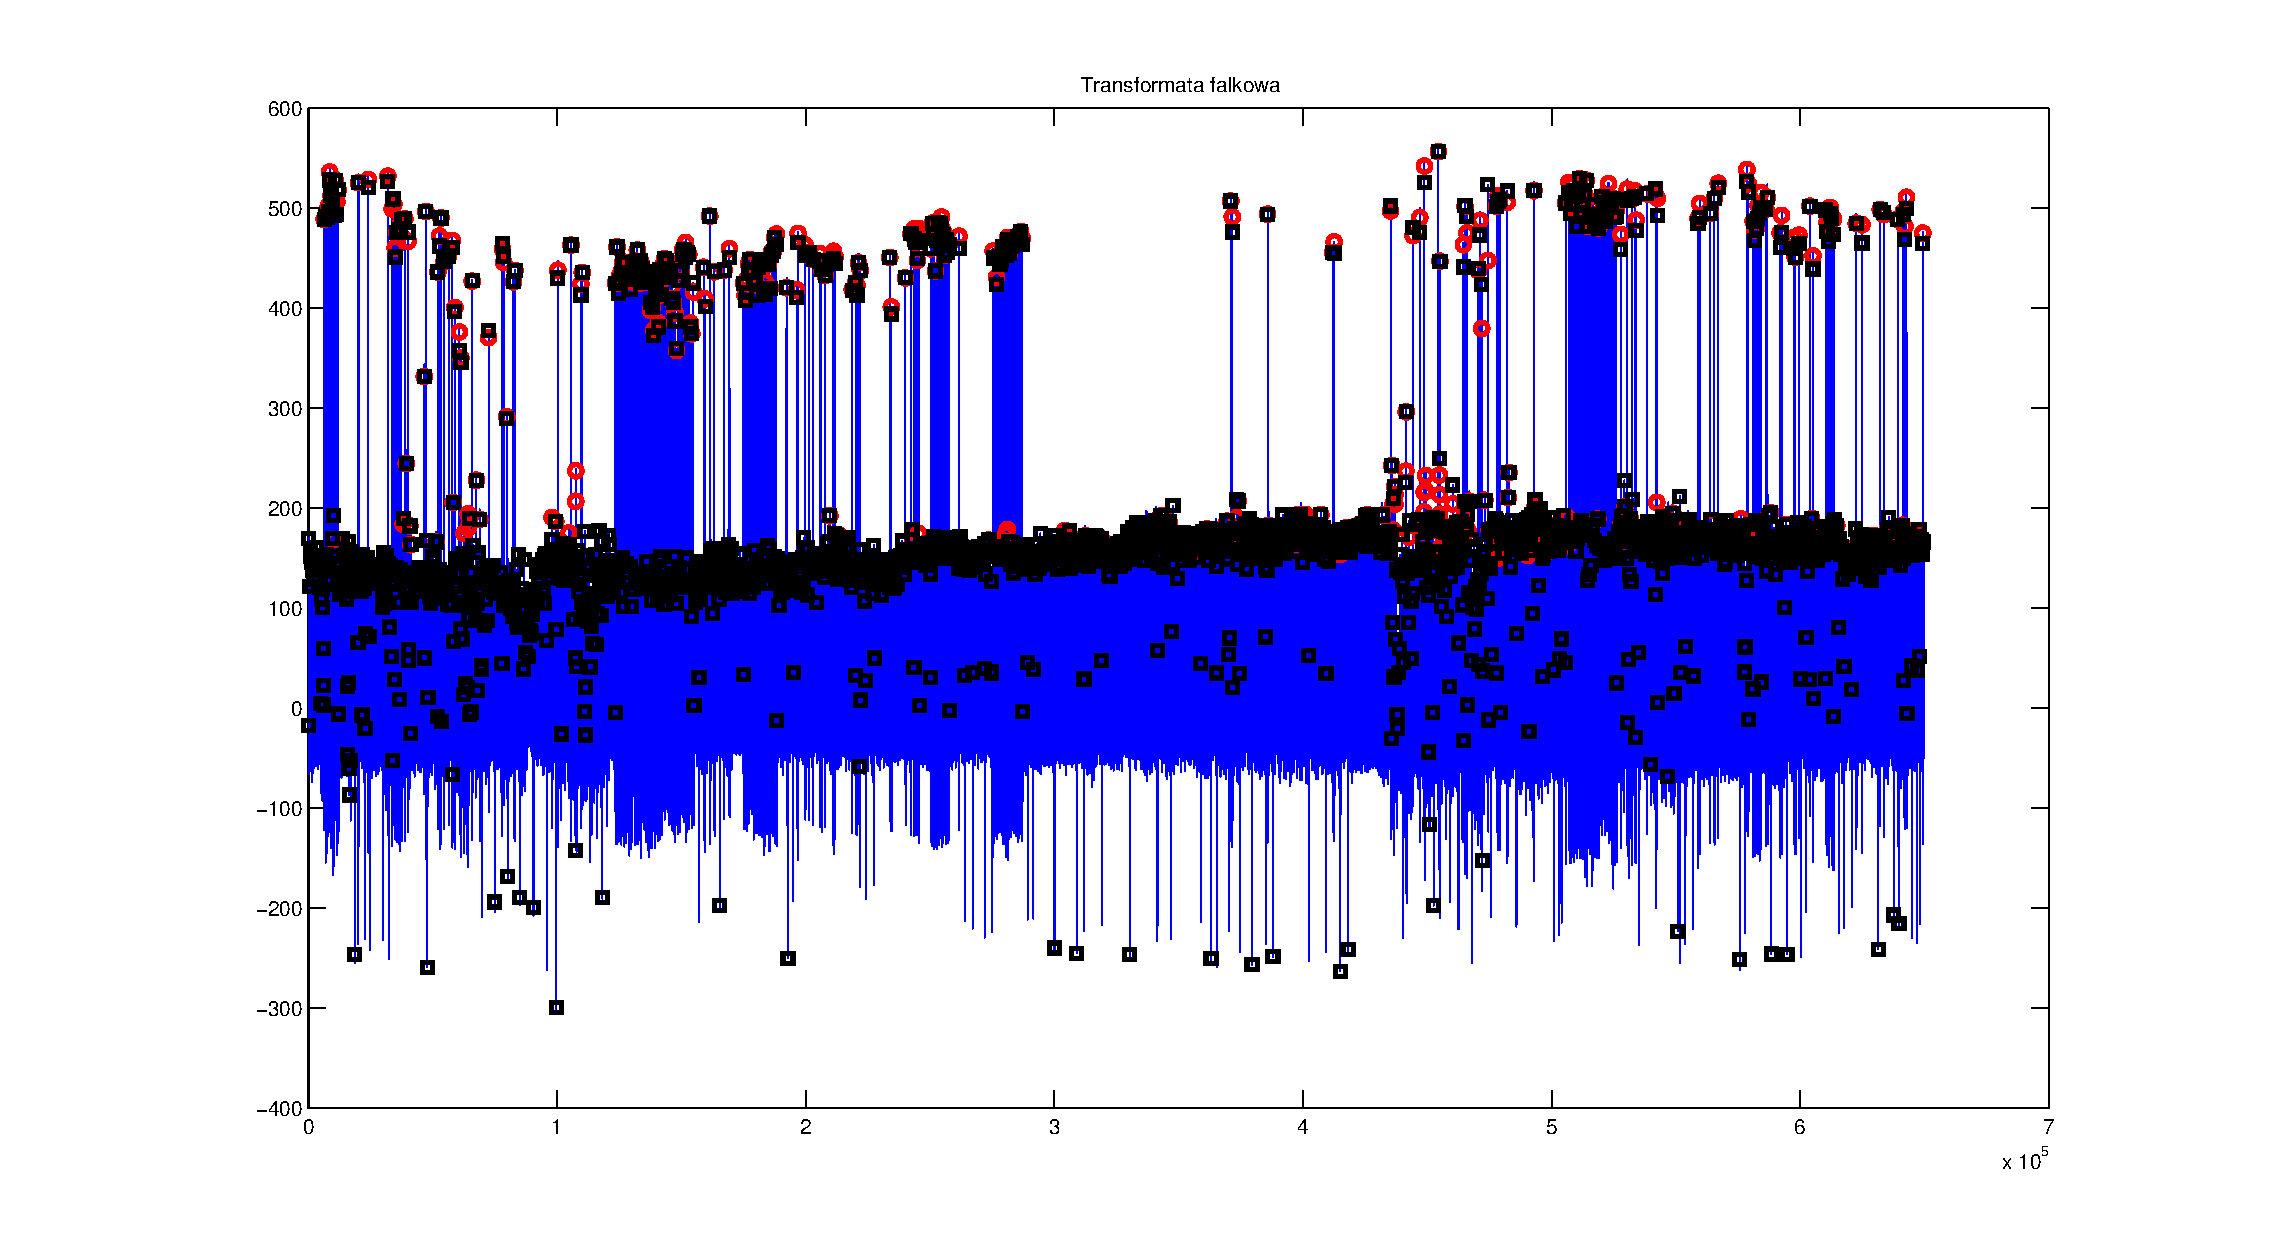
\includegraphics[scale=0.35]{R_PEAKS/wektorowe/228_falka_calosc.eps}
\caption{Sygnał nr 228 z naniesionymi pikami R - transformata falkowa}
\label{fig:228WC}
\end{figure}

\begin{figure}[H]
\centering
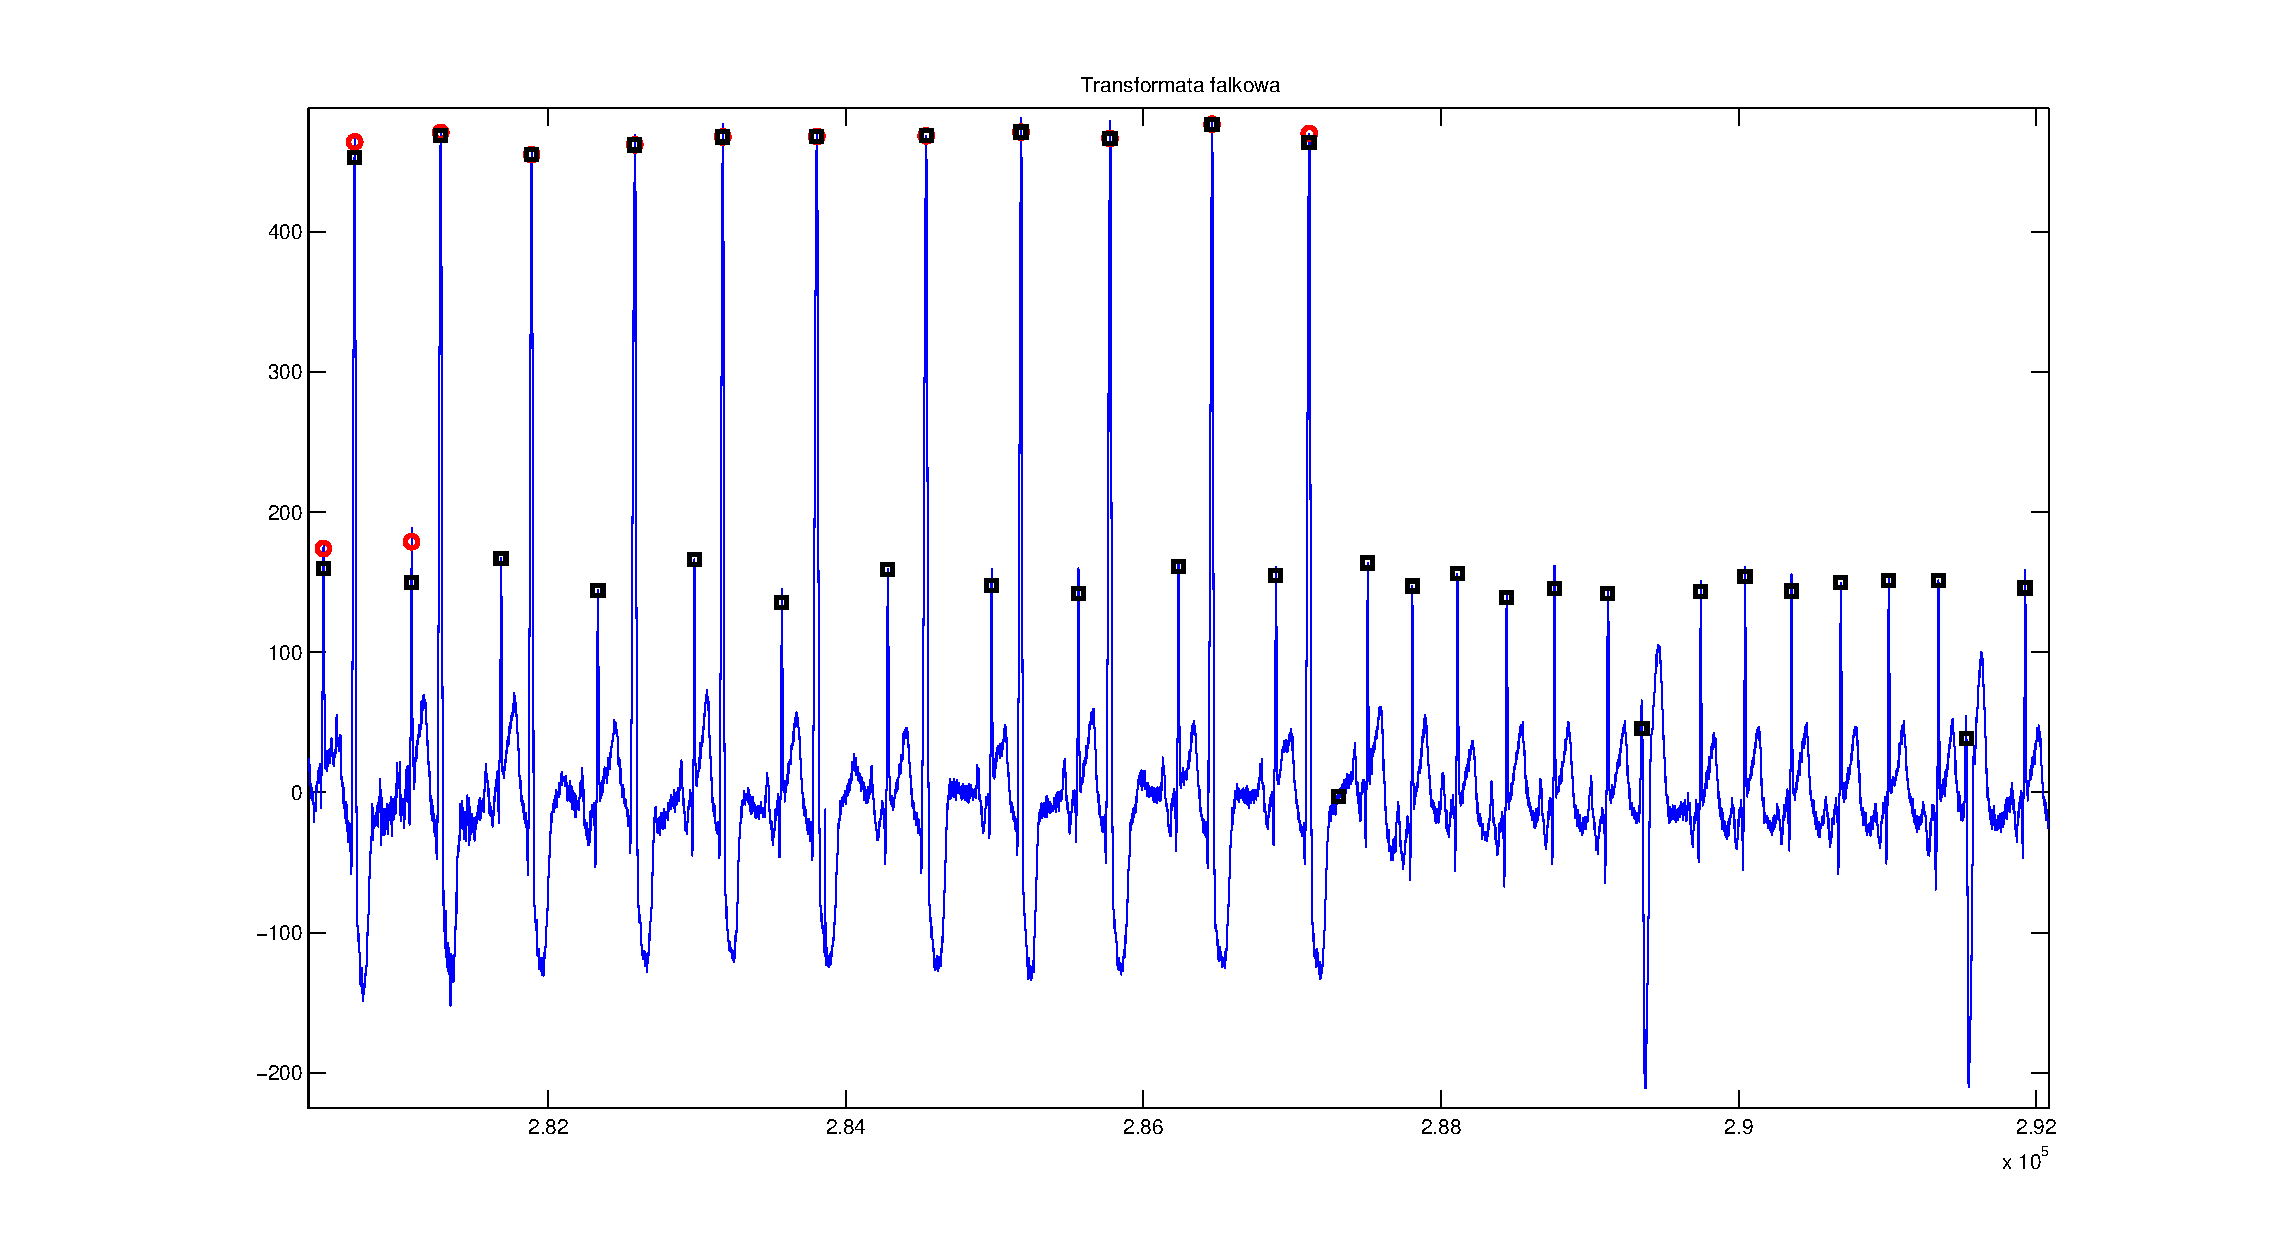
\includegraphics[scale=0.35]{R_PEAKS/wektorowe/228_falka_fragment.eps}
\caption{Fragment sygnału nr 228 - transformata falkowa}
\label{fig:228WF}
\end{figure}
\end{enumerate}
\end{itemize}
\newpage
\subsection{Diagramy klas}
\begin{tikzpicture}
  \begin{class}[text width=10cm]{RpeaksModule}{0,0}
    \attribute{SAFETYCOEFFICIENT : static const double = 0.8}
    \attribute{MAXBPM : static const unsigned short = 220}
    \attribute{THRESHOLDDIVISOR : static const double = 20}
    \attribute{PTLPM : static const unsigned int = 9}
    \attribute{PTHPM: static const unsigned int = 56}
    \attribute{PTMWN: static const unsigned int = 58}
    \attribute{filteredSignal : QVector<double>}
    \attribute{ecgSignal : const QVector<double> \&}
    \attribute{itVect : QVector<unsigned int>}
    \attribute{frequency : double}
    
	\operation{fft(x, result)}
    \operation{ifft(x, result)}
    \operation{fftHilbertWindowed(x, result, windowlength, windowoverlap)}
    \operation{fftHilbert(x, result)}
    \operation{setHilbertRPeaks(peaks, dt)}
    \operation{PTLowPassFilter(data, reset): double}
    \operation{PTHighPassFilter(data, reset): double}
    \operation{PTDerivative (data, reset): double}
    \operation{PTSquaringFunction data): double}
    \operation{PTMovingWindowIntegral(data, reset): double}
    \operation{Maximum(begin, end, values): PairDoubleUnsignedInt}
    \operation{PanTompkinsDo(signal, result)}
    \operation{PanTompkinsSetPeaks(filter, movingWindow)}
    \operation{PeakMS(index, signal): PairDoubleUnsignedInt}
    \operation{QRSCheck(rpCandidate, rpLast, threshold, slope): int}
    \operation{falka(x, result)}
    \operation{getEvenSamples(x, result)}
    \operation{getOddSamples(x, result)}
    \operation{findGreaterEqualThan(x, coeff, result)}  
    \operation{RpeaksModule(filteredSignal, freq)}
	\operation{hilbert()}
	\operation{panTompkins()}
	\operation{wavelet()}
	\operation{getPeaksIter(): const RpeaksIterVector \&}
	\operation{getPeaksIndex(): const QVector<unsigned int> \&}
	\operation{ecgBegin(): const RpeaksIter}
  \end{class}
\end{tikzpicture}\\

\noindent \begin{tikzpicture}
  \begin{class}{DiffSorter}{0,0}
    \operation{DiffSorter()};
    \operation{operator()(a, b): bool};
  \end{class}
\end{tikzpicture}\\

\noindent \begin{tikzpicture}
  \begin{class}{PeaksCutSorter}{0,0}
    \operation{PeaksCutSorter(scope)};
    \operation{operator()(a, b): bool};
  \end{class}
\end{tikzpicture}

\newpage
\subsection{Literatura}
[1] Farahabadi A., Farahabadi E., Parsa M. Mahjoob1, Rabbani Hossein. R Peak Detection in Electrocardiogram Signal Based on an Optimal Combination of Wavelet Transform, Hilbert Transform, and Adaptive Thresholding. \textit{Journal of Medical Signals \& Sensors} 2011, nr 2, s. 91-98.\\

\noindent [2] Augustyniak Piotr. \textit{Przetwarzanie sygnałów elektrodiagnostycznych}. Kraków, Uczelniane Wydawnictwo Naukowo-Dydaktyczne, 2001, ISBN 83-88400-37-2.\\

\noindent [3] Pięciak Tomasz, \textit{Elektrokardiografia (EKG)}.\\

\noindent [4] Goszcz Sławomir, Kokoć Kamil. \textit{Detekcja i synchronizacja reprezentacji uderzeń serca (zespół QRS)}.\\

\noindent [5] Kasperczyk Paweł, Pękala Kamil. \textit{Raport z modułu obliczeniowego R\_PEAKS}. Kraków 2013.\\

\noindent [6] Hennig Carsten, Köhler Bert-Uwe, Orglmeister Reinhold. The Principles ofSoftware QRS Detection. \textit{IEEE ENGINEERING IN MEDICINE AND BIOLOGY}, January/February 2002.\\

\noindent [7] Bhujanga Rao A., Narayana K.V.L., Wavelet based QRS detection in ECG using MATLAB. \textit{Innovative Systems Design and Engineering} 2011, nr 7, s.\\ 60-69.\\

\noindent [8] Simranjit Singh Kohli, Nikunj Makwana, Nishant Mishra, Balwalli Sagar. Hilbert Transform Based Adaptive ECG R-Peak Detection Technique. \textit{International Journal of Electrical and Computer Engineering (IJECE)} 2012, nr 5, s. 639-643.
\section{Moduł VCG\_T\_LOOP}

\section{Moduł SIG\_EDR}
\subsection{Badania literaturowe}
		Moduł SIG\_EDR jest odpowiedzialny za wyodrębnienie sygnału oddechu z elektrokardiogramu. Przykładowy przebieg EKG wraz z odpowiadającym mu sygnałem oddechowym zaprezentowany został na Rys.~\ref{fig:ecg_oddech}. Wiedza na temat sposobu oddychania pacjenta jest przydatna przy analizie długoterminowej w celu wykrycia np. bezdechów sennych. Otrzymana w ten sposób informacja nie wymaga użycia dodatkowego sprzętu, mogącego zakłócić naturalny rytm oddechowy.
\begin{figure}[ht]
\centering
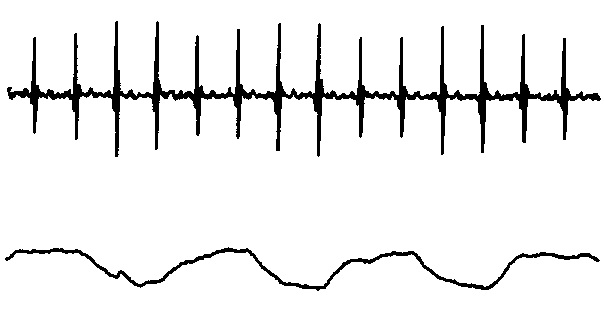
\includegraphics[width=12cm]{SIG_EDR/img/ecg_oddech.jpg}
\caption{EKG (przebieg górny) wraz z sygnałem oddechowym (przebieg dolny)}
\label{fig:ecg_oddech}
\end{figure}
 
		Sposób podejścia do problemu nie zmienił się znacznie w przeciągu lat. Istnieje kilka metod, które zyskały uznanie ze względu na swoją skuteczność tudzież prostotę obliczeniową i łatwość implementacji.
	   
		Pierwszą z nich jest metoda zaproponowana przez Felblinger et al. Polega ona na badaniu amplitudy pików R. Metoda ta wykorzystuje fakt, iż spośród wszystkich faz  EKG piki R podlegają największej modulacji podczas oddychania (w wyniku zmiany impedancji klatki piersiowej). W momencie nabrania powietrza oraz trzymania go w klatce piersiowej jej impedancja rośnie, przez co amplituda pików R maleje, odwrotnie w momencie wydychania – amplituda rośnie. Przekłada się ona zatem bezpośrednio na sposób oddychania. Aby otrzymać ciągły sygnał oddechowy pacjenta należy wykonać interpolację pików R funkcjami sklejanymi (sygnał może zostać poprawnie odtworzony, gdyż prawie zawsze częstość skurczów serca jest przynajmniej dwa razy większa od częstości oddychania – zostaje spełnione twierdzenie o próbkowaniu).  Otrzymany w ten sposób sygnał reprezentuje sposób oddychania pacjenta. Algorytm ten jest łatwy w implementacji oraz dosyć efektywny, wymaga jednak podania dobrze przefiltrowanego sygnału EKG na wejście (niezwykle istotna jest eliminacja falowania izolinii).
	   
		Kolejna metoda również opiera się na badaniu pików R. Tutaj jednak liczony jest czas trwania fali R. W tym celu w pierwszej kolejności liczona jest pochodna sygnału EKG w oknie czasowym o długości 40 ms (+/- 20 ms od piku R). Pochodna ta generuje jedno minimum oraz jedno maksimum lokalne (dla danego piku R). Wartości różnic czasowych pomiędzy minimum a maksimum umieszcza się na wykresie w funkcji czasu wystąpienia danego piku R. Następnie otrzymane punkty interpoluje się funkcjami sklejanymi, otrzymując w ten sposób sygnał EDR. Obie przytoczone metody zostały porównane w pracy Murtaza M. Lakdawala „Derivation of the respiratory rate signal from a single lead ECG”. Została w niej również zaprezentowana metoda łącząca wyniki otrzymane z obu metod.
	   
		Jedną z bardziej znanych metod jest ta zaproponowana przez Moody et al. Wykorzystuje ona sygnał z dwóch odprowadzeń. Metodę tą, podobnie jak poprzednie, realizuje się na odfiltrowanym sygnale EKG. Sygnał oddechu wyznaczany jest na podstawie zmiany kąta nachylenia głównego wektora sercowego w stosunku do osi jednego z wyprowadzeń. W celu wyznaczenia takiego wektora należy obliczyć pole powierzchni wartości bezwzględnej z kompleksów QRS dla każdego z wyprowadzeń. Następnie, aby wyznaczyć poszukiwane nachylenie, należy obliczyć arctg ze stosunku obu otrzymanych powierzchni (Rys.~\ref{fig:moody_alg}). W ten sposób dla każdego kompleksu QRS otrzymujemy jedną wartość nachylenia głównego wektora sercowego. Aby wygenerować ciągły sygnał oddechowy należy otrzymane punkty interpolować funkcjami sklejanymi. Algorytm ten zakłada ortogonalność wyprowadzeń. Jeżeli jednak warunek ten nie jest spełniony to generowany jest stały błąd, który nie ma znaczącego wpływu na wyznaczanie nachylenia głównego wektora sercowego.
	   
\begin{figure}[ht]
\centering
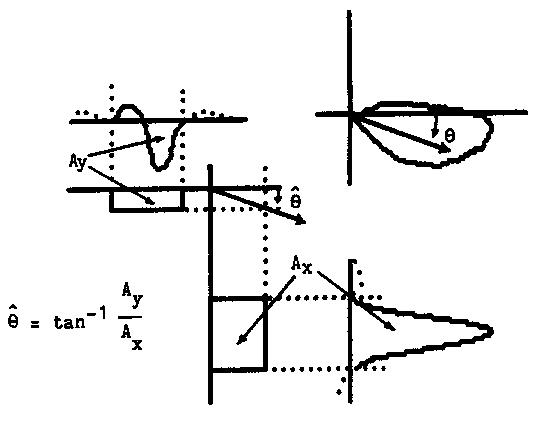
\includegraphics[width=12cm]{SIG_EDR/img/moody_alg.jpg}
\caption{Sposób wyznaczania nachylenia głównego wektora sercowego od osi jednego z wyprowadzeń.}
\label{fig:moody_alg}
\end{figure}
\newpage
		Istnieją również algorytmy wykorzystujące większą liczbę wyprowadzeń. Nie zostały one jednak rozpatrzone, ze względu na wykorzystanie w projekcie jedynie dwóch wyprowadzeń.
	   
 
\subsection{Koncepcja proponowanego rozwiązania}
 
		Z racji stosunkowo niewielkiego poziomu skomplikowania algorytmów zdecydowano się na implementację dwóch spośród wymienionych, tj. pierwszego (analiza amplitudy pików R) oraz ostatniego (badanie odchylenia głównego wektora sercowego od osi jednego z wyprowadzeń) celem porównania działania.
	   
		W przypadku pierwszego algorytmu zostały wykorzystane informacje pochodzące z modułu odpowiedzialnego za wykrywanie pików R (R\_PEAKS). Moduł ten wysyła indeksy próbek, dla których został wykryty pik R. Wartości sygnału z próbek o zadanych indeksach są następnie  interpolowane metodą funkcji sklejanych. Rząd wielomianu determinowany jest na podstawie najlepszego dopasowania do interpolowanego sygnału.   Otrzymana za pomocą interpolacji krzywa stanowi sygnał oddechowy.
 
		Drugi algorytm wykorzystuje informacje pochodzące z modułu odpowiedzialnego za detekcję punktów charakterystycznych sygnału EKG (WAVES). Schemat blokowy algorytmu został przedstawiony na poniższym rysunku (Rys.~\ref{fig:graf}):
	   
\begin{figure}[ht]
\centering
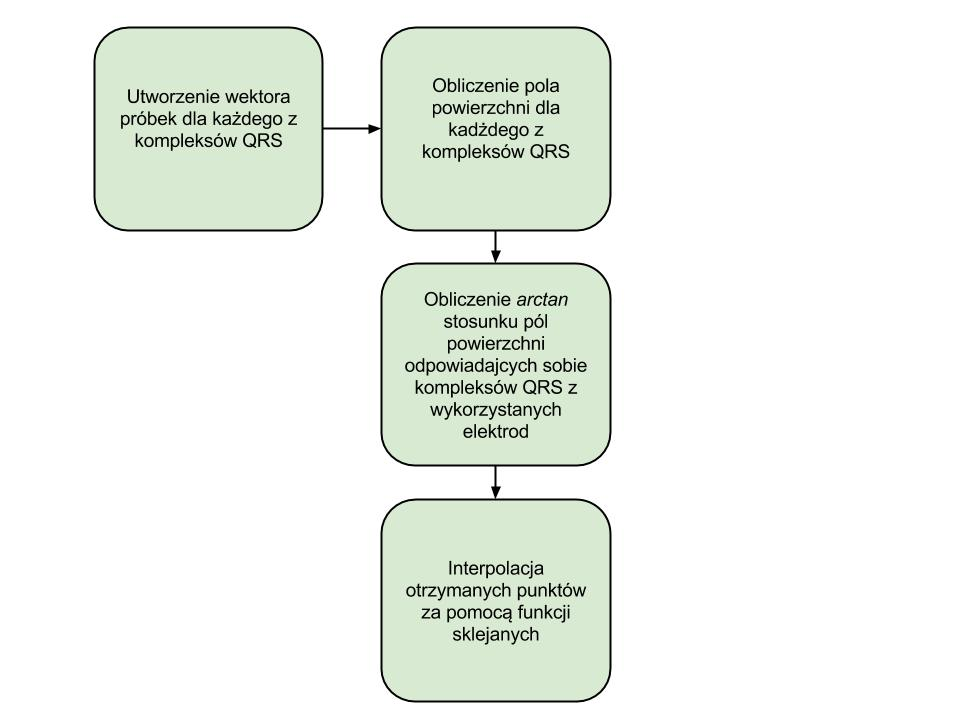
\includegraphics[width=12cm]{SIG_EDR/img/graf.jpg}
\caption{Schemat blokowy realizujący odczytywanie sygnału EDR z wykorzystaniem modułu WAVES}
\label{fig:graf}
\end{figure}   
	   
		 Na podstawie otrzymanych punktów QRSonset oraz QRSend wyznaczane jest pole powierzchni każdego z kompleksów QRS, zarówno z pierwszej, jak i z drugiej elektrody. Pole powierzchni kompleksu jest proporcjonalne do średniej amplitudy sygnału. Zakładając ortogonalność osi wyprowadzeń, $\arctan$ ze stosunku pól powierzchni obu kompleksów daje w wyniku kąt odchylenia głównego wektora sercowego od jednej z osi wyprowadzeń. Jeżeli wyprowadzenia nie są ortogonalne pojawia się błąd pomiaru. Jest on jednak stały dla całego sygnału i nie ma wpływu na wyznaczanie sygnału oddechu pacjenta.
 
		Obie metody charakteryzują się wysoką dokładnością odtwarzania sygnału oddechowego. Nie wymagają wykonywania dużej ilości obliczeń oraz są stosunkowo proste w implementacji. Dodatkową zaletą pierwszej z nich jest wykorzystanie do obliczeń sygnału z jednego odprowadzenia.
	   
\subsection{Rezultaty i wnioski}
 
		Działanie modułu zostało przedstawione na poniższych obrazkach (Rys.~\ref{fig:aplikacja_1}) oraz Rys.~\ref{fig:aplikacja_2}).
	   
\begin{figure}[h]
\centering
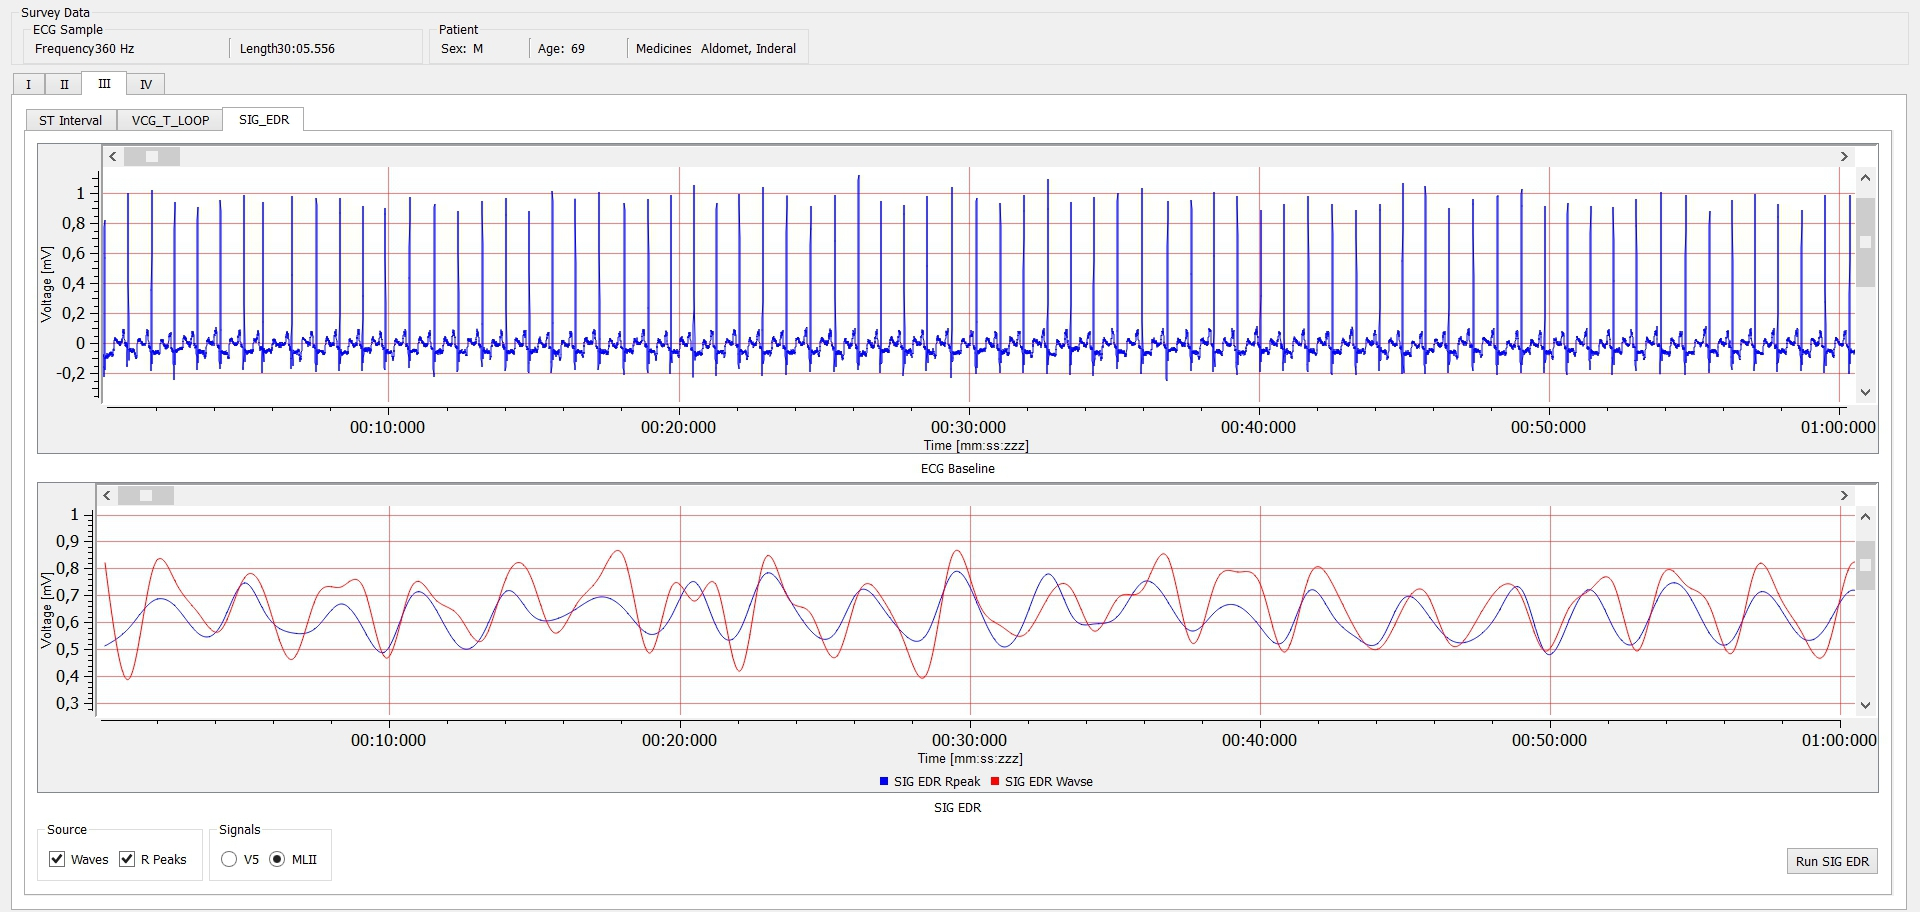
\includegraphics[width=12cm]{SIG_EDR/img/aplikacja_1_1.jpg}
\caption{Działanie modułu dla rekordu 100, pierwsza minuta sygnału}
\label{fig:aplikacja_1}
\end{figure}
 
\begin{figure}[h]
\centering
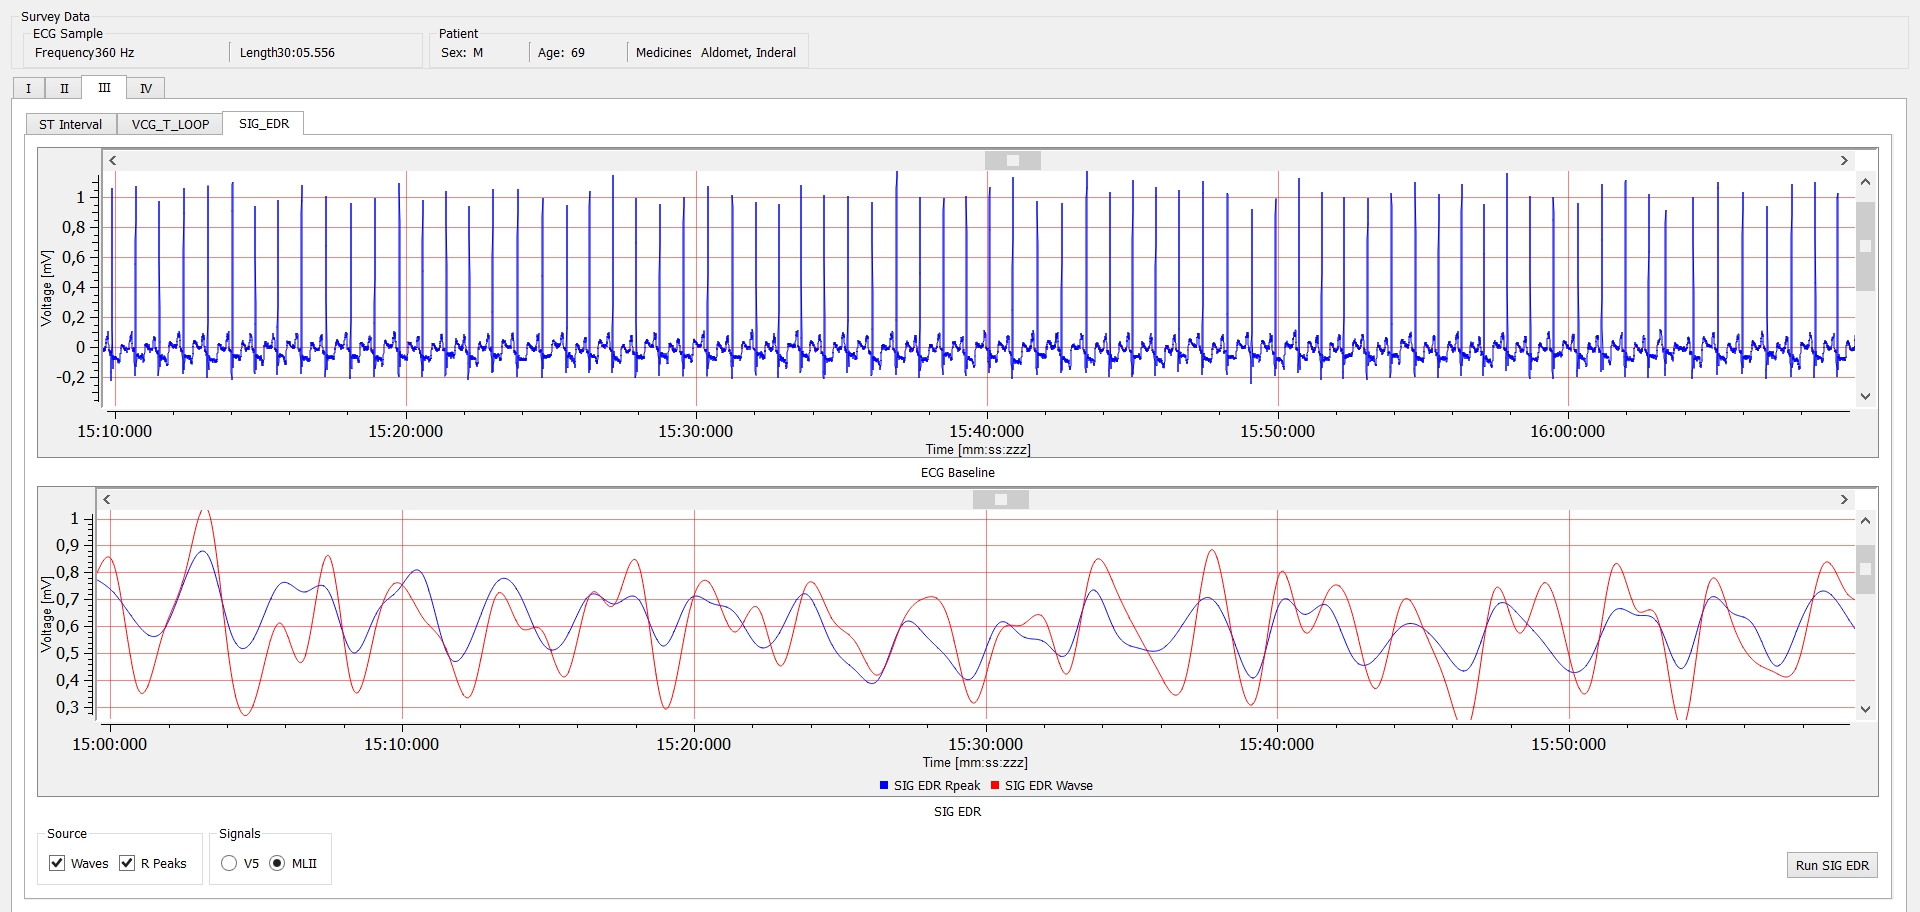
\includegraphics[width=12cm]{SIG_EDR/img/aplikacja_2_2.jpg}
\caption{Działanie modułu dla rekordu 100, piętnasta minuta sygnału}
\label{fig:aplikacja_2}
\end{figure}
 
		Niestety, z braku dostępu do rzeczywistego sygnału oddechowego dla posiadanych danych, przebiegi nie mogły zostać porównane w sposób analityczny. Jedynym sposobem sprawdzenia poprawności otrzymanego sygnału EDR było porównanie kształtu przebiegu z sygnałem ECG, a następnie porównanie z wzorcowymi sygnałami, uzyskanymi przy pomocy aparatury do mierzenia oddechu (PRT). Z tej przyczyny skupiono się na przeprowadzeniu porównania otrzymanych danych w celu weryfikacji poprawności zastosowanych algorytmów.
	   
		Dane zostały porównane w następujący sposób:
		\begin{itemize}
		\item obliczenie różnicy pomiędzy wartościami próbek stanowiących R-piki z wartościami                                   otrzymanymi w wyniku działania modułu
		\item porównanie wartości zwracanych w wyniku zastosowania drugiego algorytmu (Moody) z                               wartościami uzyskanymi z poprzedniego algorytmu
		\item obliczenie odchylenia poszczególnych różnic od średniej różnicy badanego przebiegu                          (odchylenie standardowe)
		\end{itemize}
	   
		Obliczone wartości zostały zgromadzone w tabeli zbiorczej(Tab. ~\ref{tabela_wynikow}). \newline
 
\begin{table}[ht]
\centering
\begin{tabular}{|c|c|c|c|c|c|c|c|c|c|}
\hline
	R1 & R2 & QRS & RR1 & R1Q & R2Q & WR1 & WR2 & WR3\\
\hline
		0,514&0,774&0,822&-0,260&-0,307&-0,047&0,554&0,340&0,308\\
		0,580&0,951&0,392&-0,371&0,188&0,559&0,665&0,155&0,298\\
		0,678&0,960&0,797&-0,282&-0,120&0,163&0,576&0,153&0,098\\
		0,658&0,903&0,747&-0,246&-0,090&0,156&0,540&0,123&0,105\\
		0,557&0,911&0,632&-0,354&-0,075&0,279&0,648&0,108&0,018\\
		0,591&0,888&0,572&-0,297&0,019&0,316&0,591&0,014&0,055\\
		0,747&0,991&0,769&-0,244&-0,022&0,222&0,538&0,055&0,039\\
		0,643&0,921&0,713&-0,278&-0,070&0,208&0,572&0,104&0,053\\
		0,563&0,948&0,466&-0,385&0,097&0,482&0,679&0,064&0,221\\
		0,581&0,909&0,699&-0,328&-0,118&0,210&0,622&0,151&0,051\\
		0,670&0,933&0,733&-0,263&-0,063&0,200&0,557&0,096&0,061\\
		0,571&0,878&0,723&-0,307&-0,152&0,155&0,601&0,185&0,106\\
		0,494&0,861&0,468&-0,367&0,026&0,392&0,661&0,007&0,132\\
		0,695&0,936&0,728&-0,241&-0,032&0,208&0,535&0,066&0,052\\
		0,652&0,908&0,685&-0,256&-0,033&0,223&0,550&0,067&0,038\\
		0,512&0,849&0,623&-0,337&-0,111&0,226&0,631&0,144&0,035\\
		0,557&0,919&0,536&-0,362&0,021&0,383&0,656&0,012&0,122\\
		0,718&0,957&0,774&-0,239&-0,056&0,183&0,533&0,089&0,078\\
		0,634&0,881&0,775&-0,247&-0,141&0,106&0,541&0,174&0,155\\
		0,609&0,901&0,564&-0,293&0,045&0,337&0,587&0,011&0,076\\
		0,649&0,965&0,664&-0,316&-0,015&0,301&0,610&0,048&0,041\\
		0,693&0,908&0,772&-0,215&-0,078&0,136&0,509&0,111&0,125\\
		0,647&0,883&0,832&-0,236&-0,185&0,050&0,530&0,219&0,210\\
		0,558&0,929&0,486&-0,371&0,073&0,443&0,665&0,039&0,182\\
		0,626&0,935&0,734&-0,310&-0,108&0,202&0,604&0,141&0,059\\
		0,751&0,959&0,680&-0,208&0,072&0,280&0,502&0,039&0,019\\
		0,581&0,897&0,733&-0,317&-0,153&0,164&0,611&0,186&0,097\\
		0,571&0,929&0,421&-0,358&0,151&0,509&0,652&0,117&0,248\\
		0,777&0,963&0,826&-0,186&-0,049&0,137&0,480&0,082&0,124\\
		0,703&0,911&0,697&-0,208&0,006&0,214&0,502&0,027&0,047\\
		0,567&0,915&0,632&-0,348&-0,065&0,283&0,642&0,098&0,022\\
		0,564&0,968&0,472&-0,404&0,092&0,496&0,698&0,059&0,235\\
		0,716&0,993&0,711&-0,278&0,005&0,282&0,572&0,029&0,021\\
		0,659&0,950&0,690&-0,291&-0,032&0,259&0,585&0,065&0,001\\
 
\hline
\end{tabular}
\caption{Porównanie wartości próbek R-pików z obu elektrod oraz metody wykorzystującej moduł WAVES.
			R1 - wartości próbek z pierwszej elektrody, R2 - wartości próbek z drugiej elektrody, QRS - wartości próbek otrzymanych metodą wykorzystującą moduł WAVES, RR1 - różnice pomiędzy wartościami odpowiadających próbek z R1 i R2, R1Q - różnice pomiędzy wartościami odpowiadających próbek z R1 i QRS, R2Q - różnice pomiędzy wartościami odpowiadających próbek z R2 i QRS, WR1, WR2, WR3 - odchylenia od średniej różnicy dla kolejnych par (odpowiednio RR1, R1Q oraz R2Q) }
\label{tabela_wynikow}
\end{table}
	   
 
		Przeprowadzone badania miały na celu sprawdzenie czy kształt sygnału oddechowego jest taki sam dla każdej z zastosowanych metod. Badana różnica pomiędzy poszczególnymi sygnałami EDR powinna być zatem stała, bądź jak najbardziej zbliżona do stałej. Wynika to z faktu, iż w rzeczywistości mamy do czynienia z jednym sygnałem oddechowym, który jest taki sam dla każdej z zastosowanych metod. Niezależnie od zastosowanej metody, wyniki powinny mieć podobny kształt, mogą się jednak różnić wartościami, wynikającymi z różnych odległości elektrod od serca, a tym samym mocą sygnału. Na wykresie skutkuje to wertykalnym przesunięciem przebiegu i jego lekką deformacją.
	   
		Kształt przebiegu sygnału EDR w niewielkim stopniu odbiega od kształtu sygnałów wzorcowych, otrzymanych z pneumatycznej aparatury pomiarowej. Głównymi czynnikami generującymi różnice pomiędzy sygnałami EDR są nienaturalne różnice występujące pomiędzy badanymi próbkami, a tym samym wykrytymi pikami R, które są filarem stosowanego algorytmu. Podobne problemy występują w przypadku drugiego z algorytmów, gdyż jest on zależny od obu próbek. Dodatkowo nie wszystkie wykryte obszary QRS, z których ten algorytm korzysta, są poprawne.
	   
\subsection{Diagram klasy}
\begin{tikzpicture}
%       \begin{class}[text width = 9cm]{sig_edr}{0,0}
%               \attribute{+ signal_one; : const QVector<double>}
%               \attribute{+ signal_two :const QVector<double>}
%               \attribute{+ EDRsignal_RPeaks_one : QVector<double> }
%               \attribute{+ EDRsignal_RPeaks_two : QVector<double>}
%               \attribute{+ EDRsignal_Waves : QVector<double>}
%               \attribute{+ EDRsignal : std::vector<double>}
%               \attribute{+ Integrals_one :  QVector<double>}
%               \attribute{+ Integrals_two :  QVector<double>}
%              
%               \operation{+ sig_edr(\&signal_one : const QVector<double>,\\
%                       \&signal_two : const QVector<double>)}
%               \operation{+ sig_edr(\&signal_one : const QVector<double>,\\
%                       \&signal_two : const QVector<double>,\\
%                       \&RPeaksIterators_one : const QVector<unsigned int>,\\
%                       \&RPeaksIterators_two : const QVector<unsigned int>)}
%               \operation{+ sig_edr(\&signal_one : const QVector<double>,\\
%                       \&signal_two : const QVector<double>,\\
%                       \&QRSonsetIterators_one : const vector_it,\\
%                       \&QRSonsetIterators_two : const vector_it,\\
%                       \&QRSendIterators_one : const vector_it,\\
%                       \&QRSendIterators_two : const vector_it)}
%               \operation{+ new_RPeaks_signal(\&signal_num : int,\\
%                       \&RPeaksIterators : const QVector<unsigned int>) : void}
%               \operation{+new_Waves_signal(\&QRSonsetIterators_one : const vector_it,\\
%                       \&QRSonsetIterators_two : const vector_it,\\
%                       \&QRSendIterators_one : const vector_it,\\
%                       \&QRSendIterators_two : const vector_it) : void}
%               \operation{+ retrieveEDR_QVec(\EDR_type : int,\\
%                       \&signal_num : int) : QVector<double>*}
%               \operation{+ retrieveEDR_StdVec(\EDR_type : int,\\
%                       \&signal_num : int) : std::vector<double>*}
%               \operation{- integral( &value : QVector<double>) : double}
%               \operation{- calculate_signal_from_QRS(\&QRSIntegrals_one : const QVector<double>,\\
%                       \&QRSIntegrals_two : const QVector<double>) : void}
%       \end{class}
%      
 
\end{tikzpicture}


\section{Moduł WAVES}

\subsection{Badania literaturowe}

Celem niniejszej pracy było zaimplementowanie oraz przetestowanie działania algorytmu  detekcji punktów charakterystycznych syganłu EKG. W tym początku i końca zespołu QRS (QRS-onset i QRS-end) oraz fali P (P-onset i P-end). Numery próbek załamków R przyjmowane są  jako dane wejściowe wraz z przefiltrowanym sygnałem. Graficznie opisywane punkty przedstawione zostały na rysunku ~\ref{fig:Waves_EKG}.


\begin{figure}[h]
\centering
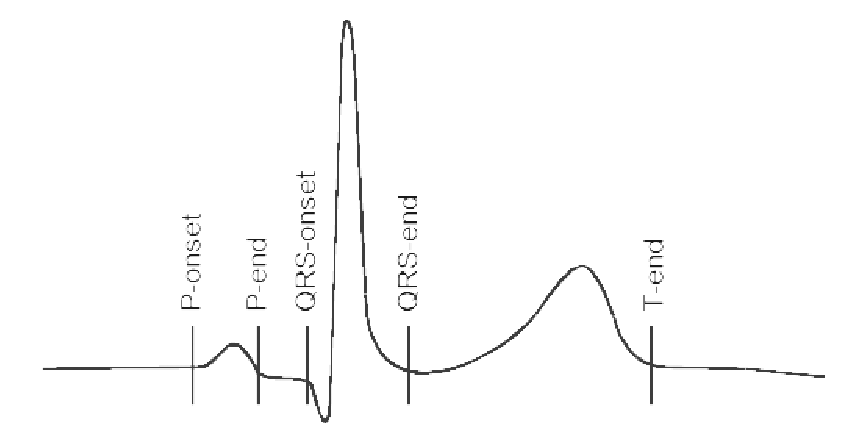
\includegraphics[width=\textwidth,keepaspectratio] {Waves/img/EKG_pts.eps}
\caption{Sygnał EKG z punktami charakterystycznymi. Źródło: \cite{Waves_PSED}}
\label{fig:Waves_EKG}
\end{figure}

Zespół QRS jest fragmentem zapisu elektrokardiograficznego odpowiadającego depolaryzacji, czyli pobudzeniu prawej i lewej komory serca. Czas jego trwania oraz kształt niosą wiele informacji na temat aktualnej kondycji serca. Dzięki swojemu charakterystycznemu kształtowi oraz wysokiej energii stanowi on często podstawę wszystkich automatycznych systemów analizy sygnałów EKG. 
Mimo intensywnych prac na przestrzeni przeszło trzydziestu lat programowe wyznaczanie zespołu QRS wciąż stanowi wyzwanie dla projektantów. Bardzo duże zróżnicowanie morfologiczne analizowanych sygnałów powoduje, że do tej pory nie opracowano detektora działającego ze stu procentową dokładnością. W ostatnich latach dynamiczny rozwój techniki pozwolił na stosowanie czasochłonnych algorytmów o dużej złożoności obliczeniowej (wyjątkiem są tu urządzenia przenośne, ze względów na bateryjne zasilanie). Zaowocowało to szeregiem nowych podejść do problemu detekcji punktów charakterystycznych zespołu QRS. W literaturze odnaleźć można algorytmy oparte o sztuczne sieci neuronowe, algorytmy genetyczne, przekształcenia falkowe, banki filtrów cyfrowych, ukryte modele Markowa, transformatę Hilberta oraz heurystyczne metody, w większości oparte o nieliniowe przekształcenia \cite{Waves_TPoSQD} \cite{Waves_Pieciak}. Cechą wspólną niemal wszystkich rozwiązań jest odpowiednie przygotowanie próbek sygnału do analizy, czyli filtracja sygnału mająca na celu usunięcie zakłóceń mięśniowych, sieciowych 50/60 Hz, zmiennej impedancji elektrod oraz artefaktów powstałych wskutek ruchu pacjentów podczas badania.
Fala P odpowiada natomiast depolaryzacji przedsionków serca i w warunkach prawidłowych występuje na schemacie zapisu elektrokardiograficznego przed zespołem QRS. Stanowi ona logiczny początek pojedynczego cyklu pracy serca. Jak w przypadku zespołu QRS automatyczne wyznaczanie początku i końca fali P cieszy się wśród projektantów dużym zainteresowaniem. Podobnie nie stworzono wciąż bezbłędnego algorytmu detekcji, gdyż wykrywanie załamka P nie jest zadaniem prostym. Ma na to wpływ parę czynników, z których można wymienić: zmienną amplitudę fali, możliwą interferencję z innymi falami występującymi w sygnale EKG, a nawet czasem brak występowania. W literaturze można znaleźć wiele przykładów badających problematykę znalezienia załamka P. Stosowane na świecie metody bazują na:
\begin{itemize}
\item pochodnych sygnału \cite{Waves_ANAfPDitES}
\item transformacie fazowej sygnału \cite{Waves_aNMfADoEFPBotPT}    \cite{Waves_ProjZeszlyRok}
\item filtrowaniu sygnału filtrami górnoprzepustowymi \cite{Waves_ARPfPDaSiHR12E}
\item transformacie falkowej \cite{Waves_DoCPoEUQSWT}
\end{itemize}
W zależności od wybranej metody algorytmy różnią się między sobą dokładnością jak i złożonością obliczeniową. Autorzy algorytmu bazującego na 9 punktowej pochodnej sygnału \cite{Waves_ANAfPDitES} zapewniają o skuteczności ok 90 procent, co nie jest wartością przekonującą. W przypadku zastosowania transformaty fazowej wyniki znalezione w publikacji \cite{Waves_aNMfADoEFPBotPT} są obiecujące: ponad 98\% procentowa wykrywalność oraz mała złożoność obliczeniowa. Skuteczność algorytmu mogła być ostatecznie sprawdzona podczas realizacji Projektu EKG \cite{Waves_ProjZeszlyRok} w ramach zajęć laboratoryjnych z przedmiotu Elektroniczne systemy diagnostyki medycznej i terapii w roku 2012/2013, kiedy został on zaimplementowany właśnie do wykrywania fali P. Niestety opracowane wyniki nie dają jednoznacznej odpowiedzi na pytanie co do przydatności algorytmu. Wynika to z tego, iż w pracy \cite{Waves_ProjZeszlyRok} znajdują się jedynie procentowe wykrycia ilości początków fali i końców P  w stosunku do znalezionych załamków R w sygnale. O ile w przypadku badania jakości wykrycia zespołów QRS taka metoda jest akceptowalna, to wiązanie ilości wykrytych początków i końców fali P z ilościami wykrytych załamków R jest niewłaściwe. Nie wiadomo także, czy wykryte załamki to faktycznie załamki P, czy może kawałki uchwyconego załamka T. Dlatego też, jedynym możliwym sposobem na weryfikację algorytmu jest porównanie otrzymanych punktów z wartościami referencyjnymi, którą zaproponowano w tej pracy.

\subsection{Koncepcja proponowanego rozwiązania}

\subsubsection{QRS-onset i QRS-end}

W trakcie realizacji moduły Waves, do wyznaczenia punktów charakterystycznych zespołu QRS zdecydowano się na algorytm bazujący na wyznaczaniu wskaźnika będącego wartością obszaru wyznaczonego obwiednią analizowanego zespołu. Algorytm ten, opisany szczegółowo w pracy \cite{Waves_QRSAlg} , można podzielić na cztery etapy, które zostały opisane poniżej (Detekcja załamka R opisana w pracy \cite{Waves_QRSAlg} została pominięta gdyż pozycja załamka R przyjmowana jest jako parametr wejściowy z innego modułu). 

\begin{description}
\item[Filtracja pasmowa]
Celem filtracji jest przekształcenie sygnału faworyzując cechy zespołu QRS, jednocześnie osłabiając cechy innych elementów elektrokardiogramu i zakłóceń. Częstotliwości odcięcia filtru pasmowego są odmienne dla detekcji QRS-onset i QRS-end i wynoszą odpowiednio [0.5 40] Hz oraz [5 30] Hz. Realizację filtru oparto o algorytm FFT (ang. Fast Fourier Transform). W tym celu  
wyznaczono transformatę całego sygnału, zastąpiono niechciane częstotliwości zerami, a następnie obliczono odwrotną transformatę wykorzystując algorytm IFFT (ang. Inverse Fast Fourier Transform).

\item[Wyznaczanie Obwiedni]
Obwiednia zbudowana jest z przefiltrowanego sygnału (części rzeczywistej) oraz jego przekształcenia Hilberta (części urojonej). Transformata Hilberta rzeczywistego sygnału x(t) zdefiniowana jest wzorem ~\ref{eq:Waves_HT1}.

\begin{equation} \label{eq:Waves_HT1}
x_H = \mathcal{H}\{x(t)\}=\frac{1}{\pi}\int_{-\infty}^\infty \frac{x(\lambda)d\lambda}{t-\lambda}
\end{equation}

Zamiast korzystać bezpośrednio z definicji można także wyznaczyć ją w domenie częstotliwości zgodnie z ~\ref{eq:Waves_HT2}.

\begin{equation} \label{eq:Waves_HT2}
X_H (j \omega) = X(j \omega) \cdot [-j \cdot sgn(\omega)]
\end{equation}

Następnie jeśli jako ECG oznaczymy rzeczywistą części sygnału przefiltrowanego, a jako ECGH część urojoną przekształcenia Hilberta sygnału to obwiednie możemy zdefiniować jako ~\ref{eq:Waves_ENV}.

\begin{equation} \label{eq:Waves_ENV}
ECG_{e} (k) = \sqrt{ECG^2 (k)+ ECG_{H}^2 (k) }
\end{equation}

Rysunek ~\ref{fig:Waves_ENV} pokazuje przykładowy zespół QRS wraz z wyznaczoną dla niego obwiednią . 

\begin{figure}[h]
\centering
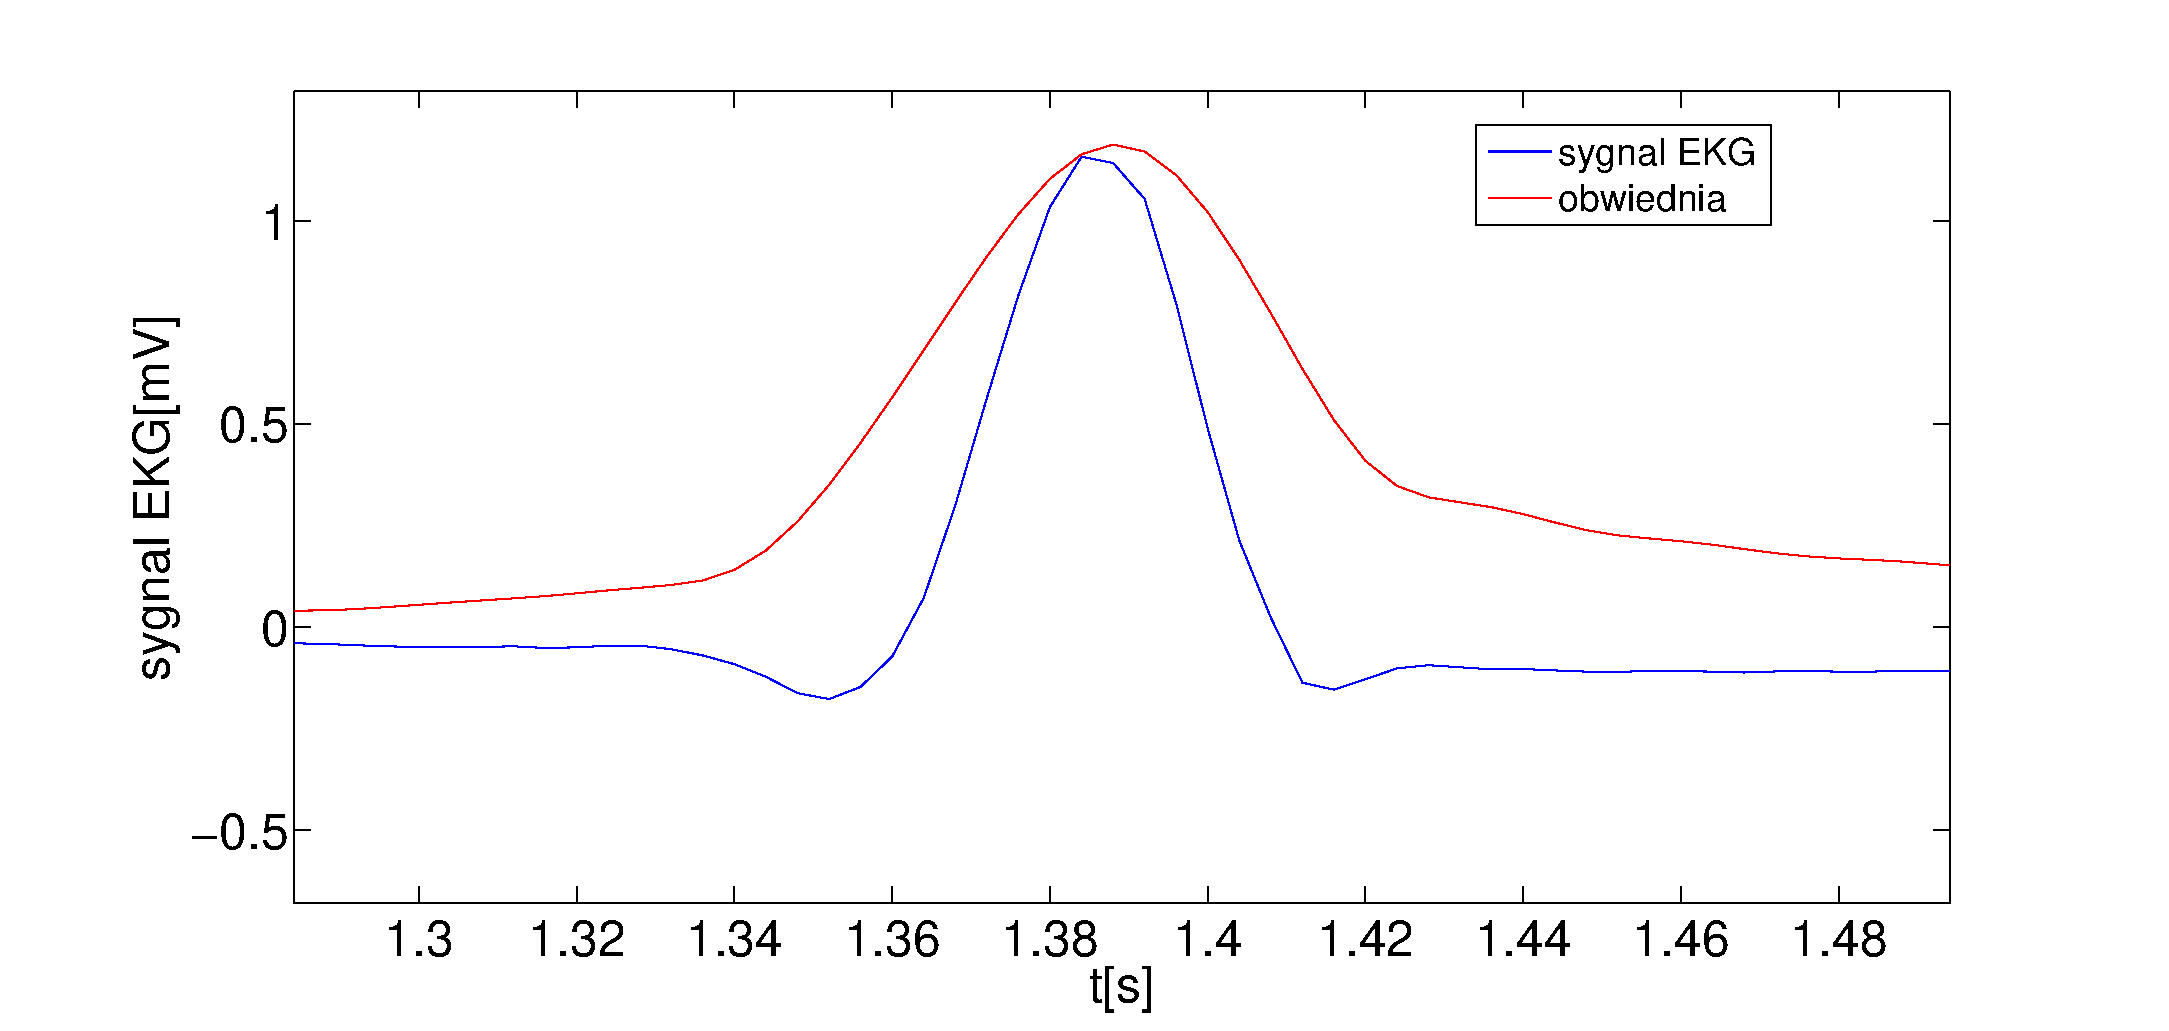
\includegraphics[scale=0.7] {Waves/img/Envelope.eps}
\caption{Sygnał EKG wraz z odpowiadającą mu obwiednią.}
\label{fig:Waves_ENV}
\end{figure}

Należy zauważyć, że wypłaszczenia obwiedni zbiegają się z początkiem i końcem zespołu QRS. Fakt ten zostanie wykorzystany w późniejszych krokach do detekcji punktów QRS-onset i QRS-end.

\item[Wyznaczanie Okna]
W celu ograniczenia zakresu poszukiwania punktów charakterystycznych zespołu QRS, zdefiniowane zostały wstępne okna w każdym cyklu pracy serca. Ze względu na czas trwania zespołu od 60 do 110 ms zdecydowano się na przeszukiwanie sygnału 100 ms przed wystąpieniem załamka R i 100 ms po nim odpowiednio dla QRS-onset i QRS-end. Taka szerokość okna powinna zapewnić objęcie pożądanych punktów, jednocześnie nie zachodząc na falę P i T. W związku z powyższym skuteczność algorytmu w sposób oczywisty zależy od poprawności wykrycia załamków R.

\item[Wyznaczanie wskaźnika powierzchni]
 Ostatnim i kluczowym krokiem algorytmu jest wyznaczenie wskaźnika powierzchni w oknie przesuwnym. Wszystkie poniższe czynności wykonywane są dla każdego cyklu serca, tylko w opisanych w poprzednim kroku oknach. Algorytm zostanie opisany na podstawie detekcji punktu QRS-end, dla ułatwienia rozpatrzony zostanie czas ciągły. Dla punktu QRS-onset postępowanie jest analogiczne i nie będzie w pracy opisane. Dla poniższych rozważań przyjęto następujące oznaczenia (patrz rysunek ~\ref{fig:Waves_A_t}):


env(t) - obwiednia sygnału w czasie, \newline
$t_1 $ i $t_2$  początek i koniec obwiedni, \newline
$t_p$ - punkt szczytowy obwiedni, \newline
$L = t_{1}-t_{2}$ - długość obwiedni pojedynczego zespołu QRS. \newline
W – szerokość okna przesuwnego

\begin{figure}[h]
\centering
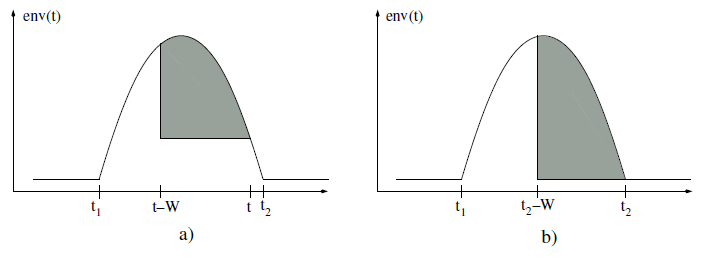
\includegraphics[width=\textwidth,keepaspectratio] {Waves/img/A_t.png}
\caption{Ilustracja wskaźnika powierzchni A(t) - szare obszary, Źródło: \cite{Waves_QRSAlg}}
\label{fig:Waves_A_t}
\end{figure}

Wykorzystany algorytm opiera się na wyznaczeniu wskaźnika A(t), który osiąga maksymalną wartość dla czasu równego $t_2$. Wyznaczany jest on przez całkowanie w oknie przesuwnym o szerokości W (wyznaczenie wartości W omówione będzie w dalszej części). W każdej chwili czasu wskaźnik może być wyliczony jako ~\ref{eq:Waves_A_t}:

\begin{equation} \label{eq:Waves_A_t}
A(t)=\int_{t-W}^t [env(\tau)-env(t)]d\tau
\end{equation}

Wskaźnik ten jest polem powierzchnią pod wykresem obwiedni w obszarze [t-W, t], ale nad poziomą linią przechodzącą przez punkt (t, env(t)). Zobrazowano to na rysunku ~\ref{fig:Waves_A_t}.
W związku z dużym zróżnicowaniem wartości L, szerokość okna W będzie osobno strojona dla każdego zespołu QRS. Jak wynika z rysunku ~\ref{fig:Waves_W0}, dla poprawnej detekcji QRS-end, wskaźnik powierzchni 2.4 powinien być wyznaczany w oknie W spełniającym zależność: $t_2 - t_p < W < L$.

\begin{figure}[h]
\centering
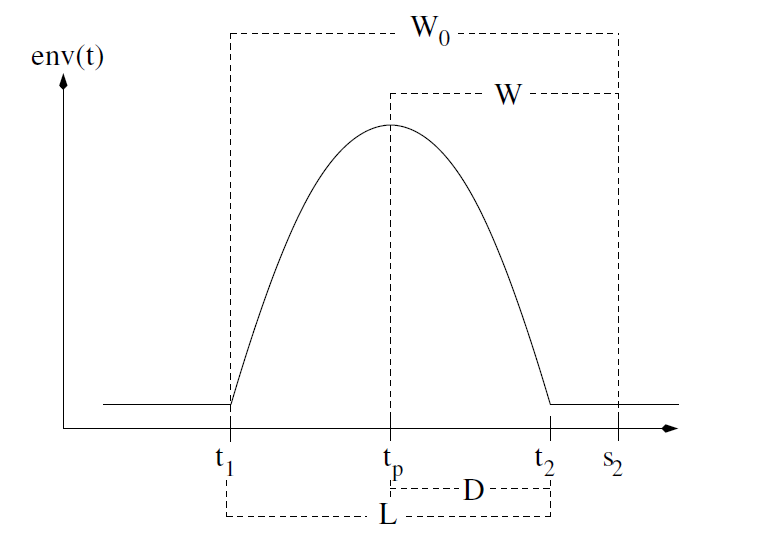
\includegraphics[width=\textwidth,keepaspectratio] {Waves/img/W0.png}
\caption{Dwuetapowy wybór okna W, Źródło: \cite{Waves_QRSAlg}}
\label{fig:Waves_W0}
\end{figure}
Kiedy wartość W jest zbyt duża, przykładowo równa $W_0$, wtedy wskaźnik przyjmuje największą wartość dla końca okna, w punkcie oznaczonym $s_2$ na rysunku ~\ref{fig:Waves_W0}. Jeśli $W_0$  nie jest zbyt duże, punkt $s_2$ powinien leżeć wystarczająco blisko $t_2$ aby spełniać warunek $s_2 - t_p < L$. W związku z tym brana jest wartości szerokości okna równa $W = s_2 - t_p$ i powtórnie wyznaczany jest wskaźnik A(t).
Podsumowując powyższe rozważania krok algorytmu można podzielić na dwie fazy: \newline
1. Obliczenie wskaźnika powierzchni dla okna przesuwnego $W=W_0$, gdzie $W_0$ jest szerokością okna opisaną w poprzednim kroku (100 ms). Wyznaczenie wartości $s_2$ maksymalizującej wskaźnik A(t) oraz wartości tp będącej maksimum obwiedni w oknie $W_0$. \newline
2. Ponowne obliczenie wskaźnika powierzchni dla okna przesuwnego o szerokości $W= s_2 - t_p$. Punkt QRS-end jest punktem maksymalizującym wskaźnik A(t).
\end{description}

\subsubsection{P-onset i P-end}
Brak rzetelnej oceny we wcześniej pracy \cite{Waves_ProjZeszlyRok} spowodował, że podjęto decyzję o ponownej implementacji algorytmu wykrywania fali P za pomocą transformaty fazowej i poprawnej weryfikacji jego skuteczności. Szczegółowe informacje co do metody można znaleźć w publikacji \cite{Waves_aNMfADoEFPBotPT}
Transformata fazowa sygnału polega na zamienieniu próbki EKG we wskaz w płaszczyźnie zespolonej wg wzoru ~\ref{eq:Waves_yN}:

\begin{equation} \label{eq:Waves_yN}
y[n]=Rv+j \cdot x[n], dla n=1,2...,N
\end{equation}

Sygnał po transformacie składa się zatem ze rzeczywistej stałej części Rv i urojonej części x[n], będącą wartością sygnału w próbce n. Moduł i faza wskazu jest obliczany jako: \newline
$M[n]=\sqrt{Rv^2+x[n]^2}$ \newline
$\phi [n]= arctan(\frac{x[n]}{Rv})$ \newline
Wykrywanie fali P dokonuje się na podstawie badania wartości fazy $\phi$, obliczanej w odpowiednim oknie.

\begin{figure}[h]
\centering
\includegraphics[width=\textwidth,keepaspectratio] {Waves/img/dzialania_fazowej.jpg}
\caption{Zależność między fazą $\phi$ a badanym sygnałem EKG. Źródło: \cite{Waves_aNMfADoEFPBotPT}  }
\label{fig:Waves_DzialFaz}
\end{figure}

Dzięki tej transformacji można odwzorować niewielką amplitudę fali P w funkcję arcustangens zawierającym wartości z przedziału [-pi/2,pi/2], co ułatwia jej wykrycie. Wykrywanie fali P za pomocą tego algorytmu polega najpierw na znalezieniu maksimum lokalnego fali P (P-middle), a następnie dokonania niezależnego wykrycia początku i końca fali (P-onset i P-end). Schematy blokowe wykrycia punktów P-middle i P-onset (P-end jest analogiczny) są zamieszczone na rysunkach ~\ref{fig:Waves_SchemPMid} oraz ~\ref{fig:Waves_SchemPOnset}

\begin{figure}[h!]
\centering
\includegraphics[scale=0.8] {Waves/img/schemat_Pmiddle.jpg}
\caption{Schemat blokowy algorytmu wykrywającego P-MIDDLE  }
\label{fig:Waves_SchemPMid}
\end{figure}

\begin{figure}[!h]
\centering
\includegraphics[scale=0.8] {Waves/img/schemat_P_oneset.jpg}
\caption{Schemat blokowy algorytmu wykrywającego P-ONSET (dla P-END jest podobny)  }
\label{fig:Waves_SchemPOnset}
\end{figure}

\subsection{Rezultaty i wnioski}
Ewentualne użycie oprogramowania do detekcji zespołów QRS w urządzeniach medycznych wymaga dokładnego testowania i oceny skuteczności. Zgodnie z literaturą \cite{Waves_TPoSQD} działanie algorytmów ocenia się na podstawie dwóch parametrów: czułości - $S_e$ (ang. sensitivity) i poprawnej wykrywalności - +P (ang positive predictivity). Wskaźniki te definiuje się odpowiednio jako ~\ref{eq:Waves_Se}, ~\ref{eq:Waves_plusP}:

\begin{equation} \label{eq:Waves_Se}
S_e=\frac{TP}{TP+FN}
\end{equation}
oraz
\begin{equation} \label{eq:Waves_plusP}
+P=\frac{TP}{TP+FP}
\end{equation}
gdzie: \newline
TP - (ang. true positive) ilość próbek wykrytych poprawnie \newline
FP - (ang. false positive) ilość próbek wykrytych błędnie \newline
FN - (ang. false negative) ilość zespołów QRS dla których algorytm nie zwrócił wyników \newline
Implementacja algorytmu zespołu QRS wyklucza możliwość występowania FN, dla każdego wejściowego załamka R zawsze zwraca parę punktów oznaczających QRS-onset o QRS-end. W związku z tym czułość algorytmu zawsze wynosi jeden. Inaczej jest dla algorytmu detekcji fali P. Ponieważ jak pisano wcześniej fala P może być przysłonięta, algorytm najpierw dokonuje oceny czy fala P istnieje. Jeśli stwierdzi brak fali P naturalnie nie wyznacza jej punktów charakterystycznych. W takiej sytuacji może zaistnieć FN, w przypadku gdy algorytm pominie  faktycznie istniejącą falę P. Dlatego, w tym przypadku wyznaczane będą oba wskaźniki. Ponadto algorytm bazuje na wartości interwału pomiędzy kolejnymi załamkami R, dlatego zwraca jedną parę mniej wykrytych początków i końców fali P niż podano wejściowych załamków R. W związku z powyższym konieczne jest też podanie kolejnych R-peaków, bez przerw. Założenie to nie jest spełnione dla wszystkich adnotacji z wykorzystanej bazy referencyjnej, dlatego do testów tego algorytmu brano tylko część adnotacji do pierwszej przerwy.   
Testy przeprowadzono wykorzystując sygnały z bazy QT database dostępnej na stronie http://physionet.org. Baza ta zawiera sto-pięć piętnastominutowych sygnałów z zaznaczonymi przez ekspertów punktami charakterystycznymi dla zespołu QRS, fali P, T oraz U. W każdym sygnale zostało oznaczone co najmniej 30 cykli. Szczegółowy opis bazy danych odnaleźć można w pracy \cite{Waves_aDfEoAfMoQaOWIitE}. Na potrzeby testów, w celu uniknięcia propagacji błędów z innych modułów wykorzystano referencyjne położenia załamków R jako daną wejściową. Punkt uznawano za poprawnie wykryty gdy jego odległość od odpowiedniego punktu referencyjnego była mniejsza od pięciu próbek. Wartości wskaźnika poprawnej wykrywalności (+P), a w przypadku fali P także czułości ($S_e$) zebrano w tabeli ~\ref{tab:Waves_tabela1} oraz tabeli ~\ref{tab:Waves_tabela2} .

\begin{table}[h!]
\caption{Wyniki algorytmu poszukującego QRS-onset i QRS-end}
\label{tab:Waves_tabela1}
\begin{tabularx}{\textwidth}{|c|X|X|X|X|X|}
  \hline
sygnał &
ilość cykli  &
TP $QRS_{onset}$ &
TP \hspace{2mm}  $   QRS_{end}$ &
+P $QRS_{onset}$  &
+P \hspace{2mm} $  QRS_{end}$  \\
\hline
sel100 & 30 & 29 & 30 & 96,67 & 100,00 \\
sel103 &
30  &
29  &
29  &
96,67 &
96,67 \\
sel114 &
50 &
37 &
47 &
74,00 &
90,00 \\
sel116 &
50 &
45 &
49 &
90,00 &
98,00 \\
sel117 &
30 &
30 &
28 &
100,00 &
93,33 \\
sel123 &
30 &
29 &
28 &
96,67 &
93,33 \\
sel213 &
30 &
24 &
25 &
80,00 &
83,33 \\
sel223 &
31 &
29 &
29 &
 93,55 &
93,55 \\
sel230 &
50 &
37 &
50 &
74,00 &
100,00 \\
sel231 &
50 &
50 &
47 &
100,00 &
94,00 \\
sel233 &
30 &
29 &
28 &
96,67 &
93,33 \\
sel803 &
30 &
27 &
29 &
90,00 &
96,67 \\
sel808 &
30 &
30 &
29 &
100,00 &
96,67 \\
sel811 &
30 &
27 &
29 &
90,00 &
96,67 \\
sel820 &
30 &
30 &
29 &
100,00 &
96,67 \\
\hline \hline
\multicolumn{4}{|r|}{średnia:}   &
 92,00 &
96,40 \\
\hline

\end{tabularx}
\end{table}

\begin{table}[!h]
\caption{Wyniki algorytmu poszukującego QRS-onset i QRS-end}
\label{tab:Waves_tabela2}
\begin{tabularx}{\textwidth}{|c|p{0.8cm}|X|X|X|p{0.7cm}|p{0.8cm}|p{0.8cm}|X|X|}
\hline
sygnał &
ilość  cykli &
TP $P_{onset}$ &
TP $P_{end}$ &
FN $P_{onset}$ &
FN $P_{end}$&
 $S_e$ $P_{onset}$ &
 $S_e$ $P_{end}$ &
+P  $P_{onset}$  &
+P  $P_{end}$ \\
\hline
sel100 &
29 &
26 &
29 &
0 &
0 &
100,00 &
100,00 &
89,66 &
100,00 \\
sel103 &
29 &
29 &
24 &
0 &
0 &
100,00 &
100,00 &
100,00  &
80,76 \\
sel114 &
29 &
18 &
23 &
2 &
2 &
90,00 &
92,00 &
66,67  &
85,19 \\
sel116 &
49 &
30 &
31 &
0 &
0 &
100,00 &
100,00 &
61,22  &
63,27 \\
sel117 &
29 &
20 &
21 &
0 &
0 &
100,00 &
100,00 &
68,97  &
72,41 \\
sel123 &
29 &
21 &
22 &
0 &
0 &
100,00 &
100,00 &
72,41  &
75,86 \\
sel213 &
29 &
3 &
20 &
0 &
0 &
100,00 &
100,00 &
10,34  &
68,97 \\
sel223 &
30 &
29 &
27 &
0 &
0 &
100,00 &
100,00 &
96,67  &
90,00 \\
sel230 &
33 &
13 &
12 &
20 &
20 &
39,39 &
37,5 &
100,00 &
92,31 \\
sel231 &
49 &
41 &
47 &
0 &
0 &
100,00 &
100,00 &
83,67  &
95,92 \\
sel233 &
29 &
15 &
14 &
0 &
0 &
100,00 &
100,00 &
51,72  &
48,28 \\
sel803 &
29 &
24 &
26 &
0 &
0 &
100,00 &
100,00 &
82,76  &
89,66 \\
sel808 &
29 &
10 &
28 &
0 &
0 &
100,00 &
100,00 &
34,48  &
96,55 \\
sel811 &
29 &
23 &
28 &
0 &
0 &
100,00 &
100,00 &
79,31  &
96,55 \\
sel820 &
27 &
21 &
24 &
1 &
1 &
95,45 &
96,00 &
77,78  &
88,89 \\
\hline \hline
\multicolumn{6}{|r|}{średnia:}   &
94,99 &
95,03 &
71,71 &
82,97 \\
\hline

\end{tabularx}
\end{table}

Jak pokazuje tabela ~\ref{tab:Waves_tabela1} algorytm detekcji punktów charakterystycznych zespołu QRS działa z zadowalającą dokładnością. Świadczy to o poprawności implementacji algorytmu w stworzonym module. Przykładowe działanie algorytmu detekcji punktów QRS-onset i QRS-end dla sygnału sel100 pokazano na rysunku ~\ref{fig:Waves_sel100}.

\begin{figure}[h!]
\centering
\includegraphics[width=\textwidth,keepaspectratio] {Waves/img/sel100.eps}
\caption{Sygnał sel100 z bazy QT-Database}
\label{fig:Waves_sel100}
\end{figure}

Rysunek ~\ref{fig:Waves_sel100} pokazuje także że jakość dostępnych adnotacji nie jest najlepsza. Punkty oznaczone jako Qrs-end znajdują się na załamkach S, co może spowodować (dla silnie ujemnych wartości załamka S) zaklasyfikowanie poprawnie wykrytego punktu jako błędny.   
Najsłabsze wyniki dla QRS-onset, różniące się o 18\% od średniej, uzyskano dla sygnału sel114. Wyniki +P dla punktu QRS-end nie spadły dla żadnego z testowanych sygnałów poniżej 90\%. Ponownie najsłabiej algorytm poradził sobie z sygnałem sel114, dla którego wynik różnił się od średniej o 6,4\%. Sytuacja taka ma miejsce ze względu na kształt sygnału sel114.
Występuje tam przy załamku R drugi, mający zbliżoną wartość, peak sygnału. Powoduje to zaburzenie kształtu obwiedni, która powinna być funkcją dzwonową obejmującą cały zespół QRS. Skutkuje to błędnym działaniem algorytmu. Sytuację przedstawia rysunek ~\ref{fig:Waves_Error}.

\begin{figure}[h!]
\centering
\includegraphics[width=\textwidth,keepaspectratio] {Waves/img/Error.eps}
\caption{Trudny przypadek dla algorytmu detekcji QRS-end oraz QRS-onset}
\label{fig:Waves_Error}
\end{figure}

Jak widać na rysunku ~\ref{fig:Waves_Error}, algorytm dla pierwszego zespołu QRS wykrywa jego koniec w miejscu, w którym ''podwojona obwiednia'' osiąga minimum. W przyszłości błąd ten można by rozwiązać badając czy obwiednia ma dwa maksima lokalne. Jeśli tak należy poszukiwać końca ''drugiej części'' obwiedni.

W przypadku fali P czułość algorytmu jest zadowalająca, choć zdarzają się rekordy, gdzie spada ona poniżej 50\% (według tabeli ~\ref{tab:Waves_tabela2}). Gorzej jest natomiast z wykrywalnością: średnio 71\% dla fali P-ONSET i prawie 83\% procent dla fali P-END. Dzieje się tak wskutek odbiegającego od oryginału kształtu załamka P. W badanych sygnałach bardzo często fala P przyjmowała kształt przedstawiony na rysunku ~\ref{fig:Waves_PrzykP}:

\begin{figure}[h!]
\centering
\includegraphics[width=\textwidth,keepaspectratio] {Waves/img/przykladowy_P.jpg}
\caption{Przykładowy załamek P z oznaczonym początkiem P-ONSET (kolor zielony), maksimum P-MIDDLE (kolor czarny) oraz końcem P-END(kolor czerwony).  }
\label{fig:Waves_PrzykP}
\end{figure}

Problem tkwi w położeniu P-MIDDLE; gdy znajduje się on zaraz na początku fali lub na jej końcu, okno (o długości 100 ms) łapie za długi odcinek sygnału leżący poza falą P i na niej może znaleźć nieprawidłowe punkty. Takie sytuacje, jak się okazało w badanych sygnałach zdarzają się bardzo często, dlatego też często punkty nie zgadzają się z punktami naniesionymi przez ekspertów. Problem nie jest łatwy do rozwiązania, gdyż stawiając ostrzejszy warunek na pochodną fazy otrzymujemy punkty P-ONSET i P-END na fali P, ale są one wtedy zbyt późne (dla początku) i zbyt wczesne dla (dla końca) w stosunku do wartości referencyjnych, więc mimo optycznego polepszenia sytuacji (wykryte punkty nie wypadają poza falę P), wykrywalność algorytmu staje się gorsza (gdyż przyjmuje się, że punkt został wykryty prawidłowo, gdy między nim a wartością referencyjną występuje maks 5 próbek różnicy. 
Doświadczenia pokazały,że algorytm w postaci proponowanej w publikacji \cite{Waves_aNMfADoEFPBotPT} może być zastosowany jedynie do zgrubnej detekcji granic fali P, gdyż nie jest wystarczająco dokładny i dla bardzo zniekształconej fali P daje słabe rezultaty. Aby zwiększyć jego wykrywalność, należało by może  wprowadzić zmienną długość okna po wykryciu punktu P-middle w zależności od zaistniałej sytuacji  lub też po wykryciu tego punktu zastosować inny algorytm.

\subsection{Diagramy klasy i sekwencji}
\subsubsection{Diagram klasy}
\begin{tikzpicture}
  \begin{class}[text width=12cm]{Waves}{0,0}
    \attribute{- qrs\_onset :  QVector<QVector<double>::const\_iterator>> }
    \attribute{- qrs\_end :  QVector<QVector<double>::const\_iterator>> }
    \attribute{- p\_onset :  QVector<QVector<double>::const\_iterator>> }
    \attribute{- p\_end :  QVector<QVector<double>::const\_iterator>> }
        \attribute{- fs :  double }

    \operation{+calculate\_waves(ECG : QVector<double> \&, R\_peaks : vector\_it\&, Fs : double)}
    \operation{+get\_qrs\_onset() : const QVector<QVector<double>::const\_iterator>> \&}
    \operation{+get\_qrs\_end() : const QVector<QVector<double>::const\_iterator>> \&}
    \operation{+get\_p\_onset() : const QVector<QVector<double>::const\_iterator>> \&}
    \operation{+get\_p\_end() : const QVector<QVector<double>::const\_iterator>> \&} 
    \operation{-set\_qrs\_onset(ECG : QVector<double>\&,R\_peaks : vector\_it\&)}
    \operation{-set\_qrs\_end(ECG : QVector<double\&,vector\_it\&)}
    \operation{-set\_p\_onset(ECG : QVector<double>\&, R\_peaks : vector\_it\&)}
    \operation{-set\_p\_end(ECG : QVector<double>\&, R\_peaks : vector\_it\&)}
        
  \end{class}
\end{tikzpicture}
\subsubsection{Diagram sekwencji}
\begin{sequencediagram}
	\newthread{t}{ : Controller}
	\newinst[2]{i}{ : Waves}

%	\begin{messcall}{t}{prepare()}{i}
%	\end{messcall}

	\begin{call}{t}{calculate\_waves()}{i}{}
		\begin{callself}{i}{set\_qrs\_onset()}{}
		\end{callself}
		\begin{callself}{i}{set\_qrs\_end()}{}
		\end{callself}		
		\begin{callself}{i}{set\_p\_onset()}{}
		\end{callself}
		\begin{callself}{i}{set\_p\_end()}{}
		\end{callself}
			
	\end{call}
	\begin{call}{t}{get\_qrs\_onset()}{i}{qrs\_onset}
	\end{call}
	\begin{call}{t}{get\_qrs\_end()}{i}{qrs\_end}
	\end{call}
	\begin{call}{t}{get\_p\_onset()}{i}{p\_onset}
		\end{call}
	\begin{call}{t}{get\_p\_end()}{i}{p\_end}

	\end{call}		
\end{sequencediagram}

%\end{sequencediagram}
\section{Moduł HRV1}



\section{Moduł QRS\_CLASS}
Zadaniem modułu R\_PEAKS jest detekcja załamków R w elektrokardiogramie. Jest to jeden z kluczowych etapów analizy sygnału EKG. Poprawne 

\section{Moduł ST\_INTERVAL}

\section{Moduł SLEEP\_APNEA}
\subsection{Badania literaturowe}
Bezdech senny, okresowe zaprzestanie oddychania podczas snu, jest często nierozpoznawalną wadą dróg oddechowych występującą u milionów ludzi na całym świecie, powodującą zwiększenie zachorowalności oraz śmiertelności. Za bezdech senny uważa się przerwy w wentylacji płuc dłuższe niż 10 sekund lub spłycenie oddechu poniżej 50\%.

Obecna technologia wykrywania bezdechu sennego wymaga monitorowania pacjenta podczas snu w specjalnie wyposażonych laboratoriach. Ze względu na koszty i niedogodności związane z badaniem polisomnograficznym,  dużo tańszym i łatwiejszym sposobem jest wdrażanie technik wykrywania dolegliwości za pomocą algorytmów specjalnych algorytmów. W ostatnich kilku latach, niektóre badania skupiały się na rozwijaniu automatycznych narzędzi do detekcji bezdechu sennego, na podstawie analizy sygnału EKG z różnymi technikami przetwarzania sygnału i rozpoznawania dolegliwości [1]. Niektóre badania stosowały funkcje wyodrębniania z sygnału EKG informacji jak HRV (zmienność rytmu zatokowego), amplitudy zespołu QRS, obszary pików R. Uzyskane wyniki pozwoliły stworzyć różne stopnie klasyfikacji między osobami zdrowymi, a cierpiącymi na bezdech senny.  Spośród różnych metod klasyfikacji można wyróżnić transformatę Fouriera, transformatę Hilberta oraz analizę czasowo-częstotliwościową. Bardzo popularną metodą jest wykorzystywanie sieci neuronowych[2], klasyfikacja na podstawie sąsiedztw – algorytm KNN (algorytm k-najbliższych sąsiadów), klasyfikacja przy pomocy SVM (maszyna wektorów nośnych) oraz Naive Bayes(naiwny klasyfikator bayesowski)[3].

Algorytmy wykorzystujące sieci neuronowe oraz metody klasyfikacji opisane wyżej, cechują się dużym skomplikowaniem. By stworzyć poprawne kryterium klasyfikacji potrzebna jest duża ilość cech, które mogą wskazać czy badana osoba cierpi na bezdech senny czy nie. Implementacja tak złożonego i rozbudowanego algorytmu pochłonęłaby zbyt dużo czasu. Ze względów czasowych oraz technicznych zdecydowano się skorzystać z algorytmu opisanego w dokumencie [4].  Metoda ta cechuje się stosunkowo łatwą i zrozumiałą implementacją. Dodatkowo osiąga zadowalające efekty - twórcy publikacji uzyskali około 90\% skuteczności w wykrywaniu dolegliwości.
Autorzy metody zauważyli, że bezdech senny zmienia dynamikę pracy serca. U ludzi chorych, w okresach długotrwałego bezdechu sennego, tętno zwykle pokazuje cykliczne wzrosty i spadki związane z fazą bezdechu i wznowienia oddychania. Cykle, które mają tendencje do drgań przy częstotliwości między 0,01 i 0,04 Hz, są charakterystyczne dla osób cierpiących na bezdech senny i nie występują u zdrowych pacjentów.

\subsection{Koncepcja proponowanego rozwiązania}
Na podstawie algorytmu opisanego w dokumencie [4] powstała koncepcja rozwiązania problemu wykrycia bezdechu sennego:
\begin{enumerate}
 \item \textbf{Obliczenie interwałów RR}
 
 Danymi wejściowymi, które były podstawą rozważań, były piki typu R. By przejść do kolejnego etapu wyznaczania bezdechu sennego należało wyznaczyć tzw. interwały RR, a więc odległości pomiędzy kolejnymi pikami R.
 \item \textbf{Zastosowanie filtru uśredniającego interwały RR}
 
 Wyznaczony sygnał okazał się mocno zaszumiony. Dalsza praca na nieczytelnym, zaszumionym sygnale wiązałaby się ze stopniowym narastaniem błędów w każdym kolejnym kroku algorytmu. By uniknąć tego niepożądanego efektu zastosowany został filtr uśredniający.
 \item \textbf{Przeprókowanie sygnału na częstotliwość 1Hz}
 
 Początkowo, uzyskany sygnał był próbkowany nierównomiernie. Uniemożliwiało to dalsze poprawne rozważania m.in. zadowalające wyznaczenie transformaty Hilberta, a w konsekwencji błędne działanie modułu. Dlatego sygnał został przepróbkowany na częstotliwość jednego herca, tak by próbki występowały w odstępach sekundowych.
 \item \textbf{Filtracja dolno i górno-przepustowa}
 
 W celu eliminacji nagłych, nienaturalnie dużych skoków amplitudy oraz wstępnej normalizacji przepróbkowanego sygnału, dokonano filtracji dolno i górno przepustowej. Sygnał po wykonaniu wszystkich poprzednich kroków był gotowy do zastosowania transformaty Hilberta.
 \item \textbf{Zastosowanie transformaty Hilberta oraz wyznaczenie sygnału amplitudowego i częstotliwościowego}
 
 Sygnał poddany został transformacie Hilberta, którą dla funkcji g(t) przedstawia równanie:
 \begin{equation}
 \widehat{g}(t) = \frac{1}{\pi}\int\limits_{-\infty}^{\infty} \frac{g(\tau)}{t-\tau} d\tau
 \end{equation}
 Jest to splot funkcji g(t) z funkcją:
 \begin{equation}
 h(t) = \frac{1}{\pi t}
 \end{equation}
 
 W każdym punkcie sygnału wyznaczane jest widmo amplitudowa i częstotliwościowe Hiberta, z których to bezpośrednio wyznaczone zostanie występowanie bezdechu sennego.
 \item \textbf{Filtracja uśredniająca oraz normalizacja sygnału amplitudowego}
 
 By uniknąć zaszumień i błędnych wyników ponownie dokonano filtracji uśredniającej. Natomiast amplituda została dodatkowo poddana operacji normalizacji. Operacja ta została zastosowana tak, by średnia wartość amplitudy w przedziale czasu równa była 1.
 \item \textbf{Obliczenie minimalnej amplitudy Hilberta oraz maksymalnej częstotliwości Hilberta}
 
 Obliczenie minimalnej amplitudy Hilberta, która była wskaźnikiem na podstawie którego stwierdzano występowanie dolegliwości wyliczono z wzoru:
 \begin{equation}
 ampl = a+\frac{b(mid +1)}{2}
 \end{equation}
  gdzie: a=0.3, b=1.85, mid - środkowa wartość między maksymalną a minimalną amplitudą.
  
 Obliczenie minimalnej częstotliwości Hilberta, która również była wskaźnikiem na podstawie którego stwierdzano występowanie bezdechu sennego:
 \begin{equation}
 freq = 0.4mid
 \end{equation}
  gdzie: mid - środkowa wartość między maksymalną a minimalną częstotliwością.
 \item \textbf{Oznaczenie próbek, w których wystąpił bezdech senny}
 Bezdech senny był wyznaczany na podstawie amplitudy i częstotliwości Hilberta. Przekroczenie przez amplitudę,wyznaczonej w poprzednim punkcie, minimalnej amplitudy Hilberta oznaczało występowanie bezdechu sennego. Podobnie z częstotliwością. W miejscach gdzie spadała poniżej maksymalnej częstotliwości Hilberta występował bezdech senny.
\end{enumerate}

\subsection{Rezultaty i wyniki}

Działanie programu oraz wizualizację danych wyjściowych przedstawiono na Rys. ~\ref{fig:gui1}
\begin{figure}[H]
\centering
\includegraphics[scale=0.4]{SLEEP_APNEA/img/gui1.png}
\caption{GUI aplikacji dla modułu SLEEP APNEA}
\label{fig:gui1}
\end{figure} 
Na wykresie powyżej linią niebieską zaznaczono znormalizowany sygnał amlitudy, linią zieloną wartość maksymalnej amplitudy hilberta oraz pionowymi, czarnymi liniami - okresy w których wykryto bezdech senny. Pod krzywymi przedstawiono rówież ocenę bezdechu sennego w dziedzinie czasu i częstotliwości.

Program został również przetestowany dla pięciu próbek danych, pobranych z internetowej bazy danych Physionet. Algorytm analizował dane próbkowane z częstotliwością 100Hz.
Na każdym z wykresów zostały przedstawione następujące elementy:
\begin{enumerate}
 \item \textbf {\color{blue}Znormalizowana amplituda sygnału}
 \item \textbf {\color{black}Maksymalna amplituda Hilberta}
 \item \textbf {\color{red}Okres bezdechu sennego}
 \item \textbf {\color{green}Okres bezdechu sennego}
 \item {Podsumowanie danych wyjściowych}
\end{enumerate}

Poniżej zamieszczono wykresy dla pięciu zestawów danych.
\newpage
\begin{figure}[H]
\centering
\includegraphics[scale=0.7, angle=90]{SLEEP_APNEA/img/apnea1.png}
\caption{Wykres końcowy programu dla danych a01}
\label{fig:apnea_1}
\end{figure} 
\newpage
\begin{figure}[H]
\centering
\includegraphics[scale=0.7, angle=90]{SLEEP_APNEA/img/apnea2.png}
\caption{Wykres końcowy programu dla danych a02}
\label{fig:apnea_2}
\end{figure}
 \newpage
\begin{figure}[H]
\centering
\includegraphics[scale=0.7, angle=90]{SLEEP_APNEA/img/apnea3.png}
\caption{Wykres końcowy programu dla danych a03}
\label{fig:apnea_3}
\end{figure} 
\newpage
\begin{figure}[H]
\centering
\includegraphics[scale=0.7, angle=90]{SLEEP_APNEA/img/apnea4.png}
\caption{Wykres końcowy programu dla danych a04}
\label{fig:apnea_4}
\end{figure}
\newpage
\begin{figure}[H]
\centering
\includegraphics[scale=0.7, angle=90]{SLEEP_APNEA/img/apnea5.png}
\caption{Wykres końcowy programu dla danych a05}
\label{fig:apnea_5}
\end{figure} 
\newpage

Poniżej przedstawiono tabelę porównawczą dla omawianych wyżej przykładów. Są w niej zawarte wyniki badań specjalistów z Physionetu oraz wyniki sporządzonego algorytmu. 


\textbf{Współczynnik} opisywany w tabeli jest liczony następująco:
 \begin{equation}
 wsp =\frac{apnea}{ (end-begin)} 
 \end{equation}
gdzie: \newline
begin - numer pierwszej próbki rekordu \newline
end - numer ostatniej próbki rekordu \newline
apnea - ilość próbek w których wykryto bezdech senny \newline


\textbf{Ilość przedziałów} mówi o liczbie niezależnych odcinków czasu w całym sygnale, gdzie wykryto bezdech senny

\begin{table}[!ht]
  \centering
  \begin{tabular}{|c|c|c|c|c|}
    \hline
  &\multicolumn{2}{|c|}{Physionet}&\multicolumn{2}{|c|}{Algorytm} \\
    \hline
Dane&Współczynnik&Ilość przedzialów&Współczynnik&Ilość przedzialów \\
    \hline
    a01 & 95,69 & 3 & 97,71 & 10 \\
    a02 & 77,61 & 11 &  69,83 & 40 \\
    a03 & 45,37 & 11 &  67,86 & 28 \\
    a04 & 91,65 & 3 & 91,41 & 8 \\
    a05 & 57,62 & 15 & 83,97 & 36 \\
    \hline
  \end{tabular}
\caption{Tabela porównawcza dla danych pobranych z Physionetu oraz danych wyjściowych algorytmu }
\end{table}
Jak można zauważyć, zaimplementowany przez nas algorytm w większości przypadków identyfikuje bezdech senny w większej ilości próbek w porównaniu z badaniami pochodzącymi z bazy Physionetu. Taka zależność może byś spowodowana:
\begin{enumerate}
 \item Błędnym wykryciem R-pików
 \item Utratą części danych po etapach filtracji i przepróbkowania
 \item Wyliczaniem progowej wartości amplitudy na podstawie stałych współczynników
\end{enumerate}

W przypadku rekordu zdrowego człowieka algorytm wykrywa bezdech senny, ze względu na to, iż wartość progowa amplitudy jest ściśle powiązana z maksymalną i minimalną wartością amplitudy przetworzonego sygnału. Aby wyeliminować ten błąd należałoby wykrywać bezdech senny nie tylko na podstawie wyliczonej wartości progowej, ale także uwzględniając zewnętrze dane statystyczne, niezależne od badanego rekordu.
\subsection{Literatura}
[1] T. Penzel, J. McNames, A. Murray, P. de Chazal, G. Moody, and B. Raymond, “Systemantic compratition of different algorithms for apnoea detection based on electrocardiogram recordings,” Med. Biol. Eng. Comput.,vol. 40, no. 4, pp. 402–407, Jul. 2002.
\newline \newline
[2] Mendez M.O., Bianchi A.M., Matteucci M., Cerutti S., Penzel T.,” Sleep Apnea Screening by Autoregressive Models From a Single ECG Lead”, IEEE Transactions on Biomedical Engineering, Vol. 52, No. 12, 2009, pp. 2838-2850 
\newline \newline
[3] Isa S.M., Fanany M.I., Jatmiko W., Arymurthy A.M., “Sleep Apnea Detection from ECG Signal: Analysis on Optimal Features, Principal Components”, and Nonlinearity, International Conference on Bioinformatics and Biomedical Engineering, 2011, pp. 1-4 
\newline \newline
[4] J. E. Mietus, C. K. Peng, P. Ch. Ivanov, A. L. Goldberger, “Detection of Obstructive Sleep Apnea from Cardiac Interbeat Interval Time Series”, Beth Israel Deaconess Medical Center and Harvard Medical School, Poston, USA
\includegraphics[scale=1.4]{SLEEP_APNEA/img/blank.png}
\subsection{Diagram klas}
\begin{tikzpicture}
  \begin{class}[text width=15cm]{SleepApnea}{0,0}
    \attribute{dataFreq : int=samplingFreqency}
    \attribute{window : int = 41}
    \attribute{lfilt : int = 32}
    \attribute{windowMedian : int = 60}

    \operation{sleepApnea(samplingFreqency : const int)}
   \operation{sleepApnea plots(tabRpeaks : QVector<unsigned int>)}
    \operation{sleepApnea output(tabRpeaks : QVector<unsigned int>)}
    \operation{guiOutput(tabRpeaks : QVector<unsigned int>)}

    \operation{RRintervals(samplingFreqency : const int)}
    \operation{averangeFilter(tab RR : QVector<QVector<double> >)}
    \operation{resample(tabRRnew : QVector<QVector<double> >)}
    \operation{HpLpFilter(\&tabRes : QVector<QVector<double> >)}
    \operation{hilbert(tabRes : QVector<QVector<double> >,\&hAmp : QVector<QVector<double> >,\&hFreq : QVector<QVector<double> >)}
    \operation{freqAmpFilter(\&hAmp : QVector<QVector<double> >,\&hFreq : QVector<QVector<double> >)}
    \operation{medianFilter(\&hAmp : QVector<QVector<double> >,\&hFreq : QVector<QVector<double> >)}
    \operation{apneaDetection(tabAmp : QVector<QVector<double> >, tabFreq : QVector<QVector<double> >)}
  \end{class}
\end{tikzpicture}
\includegraphics[scale=0.8]{SLEEP_APNEA/img/blank.png}
\section{Moduł ATRIAL\_FIBR}
\subsection{Badania literaturowe}
Celem jest wykrycie u osoby badanej migotania przedsionków (ang. \textit{Atrial Fibrillation}). 
Jest to zaburzenie polegające na nieskoordynowanym pobudzeniu przedsionków serca. 
Ryzyko zgonu u osoby chorej wzrasta dwukrotnie, a problem dotyczy $1-2\%$ ogółu populacji.
Migotanie przedsionków zazwyczaj jest bezobjawowe, zaburzenie jest wykrywane przypadkowo,
lub po udarze niedokrwiennym mózgu.
Zwykle występuje u pacjentów z organiczną chorobą serca, ale również może wystąpić u osób zdrowych.
Możliwe do zaobserwowania objawy to duszności, kołatanie serca, ból w klatce piersiowej czy zawroty głowy.

Sygnał EKG u chorego charaktreryzuje się następującymi własnościami:
\begin{itemize}
  \item brak załamków P
  \item odstępy R-R nieregularne
  \item obecna fala migotania
  \item zespoły QRS zwykle wąskie
\end{itemize}
\begin{figure}[ht]
\centering
\includegraphics{ATRIAL_FIBR/img/AF_ecg.jpg}
\caption{Sygnał EKG dla osoby chorej i prawidłowy rytm zatokowy} \label{fig:AF_ecg}
\end{figure}

Rysunek \ref{fig:AF_ecg} na górym zapisie przedstawia sygnał EKG dla osoby chorej na migotanie przedsionków,
natomiast dolny zapis prezentuje prawidłowy rytm zatokowy.
Wykres osoby chorej wyraźnie przedstawia wszystkie podane symptomy.

Literatura podawała kilka czynników mogących wskazywać na występowanie u pacjenta migotania przedsionków. 
Jeden artykuł [1] przedstawiał metodę opartą jedynie na detekcji peaków R. 
Autorzy uważali, że na podstawie jedynie nieregularnych interwałów R-R 
można z powodzeniem wykryć u badanego chorobę. 
Metoda ta polega na zaklasyfikowanie odległości jako małych, dużych i normalnych. 
Następnie przedstawienie jako procesu Markowa i porównanie do wyników osoby zdrowej miało pozwolić 
na uzyskanie ostatecznego wyniku.
Niestety, po wyliczeniu parametrów dot. bicia serca, 
okazało się, że jeden z próbnych sygnałów dostępnych w bazie Physiobank - 
iaf4\_ivc - wykazuje własności bardzo zbliżone do zdrowego człowieka.

Autorzy drugiego źródła [2], prócz wspomnianej rozszerzyli sposób rozwiązania problemu dodając następujące metody:
\begin{enumerate}
 \item \textbf{Wykrycie absencji załamka P}
 
    Po ustaleniu pewnego wzorca  P (na podstawie dużej liczby próbek), 
    zostaje porównany do sygnału osoby badanej. 
    Ilość wystąpień załamka zostaje wyznaczona na podstawie wyznaczonego progu.
 \item \textbf{Analiza aktywności przedsionków}
 
    Po usunięciu QRS-T, sygnał u osoby chorej charakteryzuje się występowaniem fali o częstotliwości 4-10 Hz. 
    Należy wykonać analizę widma -- po zastosowaniu FFT (Fast Fourier Transform) 
    trzeba sparametryzować widmo częstotliwości.  
    U osoby chorej można zaobserwować koncentrację wokół wierzchołka położonego w przedziale [4,10] Hz.
\end{enumerate}

\subsection{Koncepcja proponowanego rozwiązania}
Początkowo zasugerowani artykułem z MIT postanowiliśmy wypróbować metodę tam przedstawioną 
i ograniczyć się do analizy interwałów R-R. 
Jednak po niepowodzeniu zmuszeni byliśmy wybrać inną metodę. 
Ze względu na istotę problemu -- zdecydowaliśmy się również wykorzystać metodę wykrywania absencji P.
\paragraph{Analiza sygnału będzie więc polegała na zbadaniu występowania 2 parametrów:}
\begin{enumerate}
    \item Odległości pomiędzy załamkami R
    \item Brak załamków P
\end{enumerate}
Gdy oba warunki zostaną spełnione, uznamy, że występuje migotanie przedsionków w danym fragmencie sygnału.
Okno analizowanego sygnału wynosi 100 uderzeń serca - 60 załamków P.
Wartość ta musiała być wystarczająco duża, by móc odpowiednio zbadać wszystkie wartości.
Jednak przy zbyt dużym oknie wynik mógłby zostać błędnie zinterpretowany.

\paragraph{Parametry związane z rytmem serca}
Informację na temat położenia w czasie peaków R otrzymamy z modułu QRS Complex. 
Na jej podstawie zakwalifikujemy każdy przedział RR jako krótki (poniżej 85\% średniej), 
średni, oraz długi (powyżej 115\% średniej). 
Następnie wyliczymy prawdopodobieństwo przejść między poszczególnymi stanami. 
Finalnie otrzymamy z tego dwa parametry - 
entropię sygnału oraz odchylenie sygnału od średniej macierzy zdrowego człowieka metodą Jensena-Shannona.
\begin{figure}[ht]
\centering
\includegraphics[width=12cm]{ATRIAL_FIBR/img/RRMethodFlow.jpg}
\end{figure}

\begin{table}[!ht]
  \centering
  \begin{tabular}{|r|ccc|}
    \hline 
    & S & M & L \\
    \hline
    S & 0.005 & 0.023 & 0.006 \\
    M & 0.007 & 0.914 & 0.013 \\
    L & 0.019 & 0.006 & 0.003 \\
    \hline
  \end{tabular}
  \caption[Macierz Markowa - zdrowy człowiek]
          {Prawdopodobieństwo zmiany długości dystansu RR w przypadku zdrowego człowieka. 
            S - dystans krótki (mniej niż 85\% średniego), 
            M - średni, L - długi (ponad 115\% średniego)}
\end{table}

\begin{table}[!ht]
  \centering
  \begin{tabular}{|r|ccc|}
    \hline 
    & S & M & L \\
    \hline
    S & 0.056 & 0.114 & 0.062 \\
    M & 0.101 & 0.350 & 0.096 \\
    L & 0.060 & 0.114 & 0.035 \\
    \hline
  \end{tabular}
  \caption[Macierz Markowa - chory człowiek]{Uśredniona macierz Markowa dla ludzi chorych na migotanie przedsionków}
\end{table}

Prawdopodobieństwo przejścia ze stanu R (regular) do kolejnego R wynosi:
\begin{equation}
P(R|R) = \frac{P(R,R)}{P(R)}
\end{equation}

Jako miary opisującej odległość między macierzami początkowo, zgodnie z zaleceniami pozycji \cite{Pedrycz}, 
chcieliśmy użyć dywergencji Kullbacka-Leiblera:
\begin{equation}
F_{KL}(P(E_i,E_j),\overline{P_{AF}(E_i,E_j)}) = \sum_{i=1}^3\sum_{j=1}^3P(E_j, E_j) \log\left(\frac{P(E_i, E_j)}{P_{AF}(E_i,E_j)} \right)
\end{equation}
natomiast ze względu na to, że jest asymetryczna, czyli de facto nie jest metryką, postanowiliśmy skorzystać z dywergencji \textbf{Jensena-Shannona}. 
Bazuje na powyższej dywergencji, z pewnymi znaczącymi różnicami.
Jest symetryczna i zawsze ma skończoną wartość.
Pierwiastek kwadratowy dywergencji Jensena-Shannona jest metryką zwaną dystansem Jensena-Shannona.
\begin{equation}
F_{JS} = \frac{1}{2}F_{KL}(P(E_i,E_j),M)+\frac{1}{2}F_{KL}(\overline{P_{AF}(E_i,E_j)},M)
\end{equation}
gdzie $$M = \frac{1}{2}(P(E_i,E_j)+\overline{P_{AF}(E_i,E_j)})$$

W przypadku entropii skorzystaliśmy ze standardowej definicji:
\begin{equation}
H = \sum_{i=1}^3 P(E_j|E_i) 
\end{equation}

\begin{equation}
H(E_j) = - \sum_{j=1}^3P(E_j|E_i)\log_2P(E_j|E_i)
\end{equation}
Metoda została przez nas wstępnie przetestowana przy użyciu aplikacji napisanej w języku programowania Julia. 
Pozwoliło to nam wysnuć pierwsze wnioski z wykresu~\ref{fig:RRResults}.
Zielone kropki przedstawiają parametry dla sygnałów z bazy Physiobank zebranych od zdrowych ludzi,
czerwone natomiast pochodzą od chorych na migotanie przedsionków. 
Niestety nie jest możliwe oddzielenie puli kropek zielonych od czerwonych jedną linią, 
dlatego potrzebujemy dodatkowego parametru.

\begin{figure}[ht]
\centering
\includegraphics[width=12cm]{ATRIAL_FIBR/img/RRResults.jpg}
\caption{Entropia i dywergencja dla danych Physiobank}
\label{fig:RRResults}
\end{figure}

\paragraph{Detekcja absencji P}
Z modułu WAVES otrzymamy informację na temat położenia początkowego i końcowego załamka P. 
Na tej podstawie wyliczymy średni przebieg tej fali u zdrowego człowieka. 
Następnie przy użyciu oszacowanego progu wyliczymy procentową absencję fali P w zadanym sygnale, 
która będzie stanowiła kolejny współczynnik.
\begin{figure}
  \centering
  \includegraphics[width=12cm]{ATRIAL_FIBR/img/PMethodFlow.png}
  \caption{Algorytm wyliczenia współczynnika występowania fali P.}
\end{figure}

Wyliczenie współczynnika korelacji:
\begin{equation}
cc(i) = |\mathrm{corr\:coef}(P_\mathrm{wave}(i),\: \overline{P_\mathrm{wave}(i)})|, \quad i = 1,\ldots,n\; \mathrm{beats}
\end{equation}
\begin{equation}
  |\mathrm{corr\:coef}(x,y)| = 
  \frac
      {\sum_{i=1}^{n}(x(i) - \overline{x})(y(i) - \overline{y})}
      {
        \sqrt{\sum_{i=1}^{n}(x(i) - \overline{x})}
        \sqrt{\sum_{i=1}^{n}(y(i) - \overline{y})}
      }
\end{equation}
Za wykrytą falę P uznajemy tę, dla której współczynnik korelacji wynosi co najmniej $0.2$.
Stosunek liczby wykrytych fal P do liczby wszystkich okresów PQRST jest poszukiwanym współczynnikiem.

Badanie przeprowadzane jest dla pewnych okien czasowych

\subsection{Rezultaty i wnioski}
Zaproponowane przez nas metody zostały poprawnie zaimplementowane w języku C++ oraz zintegrowane z główną linią projektu.
Integralną częścią dostarczonego przez zespół kodu był zestaw testów jednostkowych napisanych 
z wykorzystaniem frameworka QtTest.

Zgodnie z koncepcją proponowanego rozwiązania, ocena prawdopodobieństwa zachorowania pacjenta na migotanie przedsionków
jest średnią ważoną z następujących parametrów:
\begin{itemize}
 \item \textbf{Dywergencja Jensena-Shannona} między wzorcową macierzą Markowa opisującą prawdopodobieństwo przejść między stanami,
 a macierzą wyliczoną dla danego pacjenta. 
 Dywergencja $0$ oznacza, że macierz jest identyczna z wzorcową. 
 
 \item \textbf{Entropia macierzy Markowa}.
 Wartość $0$ oznacza, że wszystkie wartości dystansów między falami R mieszczą się w przedziale $[85\%,115\%]$ wartości średniej.
 Z drugiej strony, wartość $1$ mówi o dużej nieregularności występowania fali R, 
 co jest symptomatyczne dla osób cierpiących na migotanie przedsionków.
 
 \item \textbf{Współczynnik zaniku fali P}. 
 Stosunek liczby okresów PQRST w których fala P występuje, do całkowitej liczby tych okresów.
 Za występowanie fali P uznajemy sytuację, w której korelacja między sygnałem w przedziale otrzymanym z modułu WAVES,
 a sygnałem wzorcowym jest większa od $0.2$.
 
\end{itemize}
Po zaaplikowaniu wyżej wspomnianych metod dla wzorcowych sygnałów z bazy Physiobank, 
można stwierdzić, że program dokonuje detekcji poprawnie. 
Właściwie dla wiekszości przypadków wystarczająca jest sama analiza rytmu bicia serca (dystansów R-R).
Zastosowanie drugiej metody związanej z absencją fali P dodatkowo zwiększyło skuteczność wykrywania choroby.

\paragraph{Weryfikacja na podstawie otrzymanych danych}

\begin{table}[ht]

\centering
    \begin{tabular}{c c c c c}
    \hline \hline
    Numer próbki & Absencja fali P &Dywergencja & Entropia &Chory \\
    \hline
    101 &0.20 &0.10 &0.71 &NIE\\
    105 &0.97 &0.04 &0.34 &NIE\\
    106 &0.83 &0.49 &0.95 &TAK\\
    107 &0.78 &0.05 &0.57 &NIE\\
    108 &0.87 &0.56 &0.95 &TAK\\
    109 &0.86 &0.07 &0.65 &NIE\\
    111 &0.18 &0.34 &0.96 &NIE\\
    112 &0.68 &0.05 &0.00 &NIE\\
    113 &0.13 &0.07 &0.72 &NIE\\
    115 &0.46 &0.14 &0.78 &NIE\\
    116 &0.85 &0.07 &0.59 &NIE\\
    118 &0.81 &0.06 &0.65 &NIE\\
    119 &0.99 &0.46 &1.00 &TAK\\
    121 &0.46 &0.39 &0.94 &NIE\\
    122 &0.88 &0.04 &0.10 &NIE\\
    200 &0.67 &0.42 &1.01 &NIE\\
    201 &0.64 &0.52 &0.92 &NIE\\
    202 &0.66 &0.22 &1.01 &NIE\\
    203 &0.72 &0.43 &1.04 &TAK\\
    \hline
    \end{tabular}
    \caption{Rezultaty uzyskane dla poszczególnych danych}\label{table:wynikiAtrialFibr}
\end{table}

Moduł jest zależny od wyników uzyskanych od innych. 
Gdyby wszystkie dane były dostarczone wcześniej, można by było wygenerować średnią falę P ze wszystkich sygnałów.
Dodatkowo, dla różnych elektrod fala P różni się kształtem i nie da się dobrać jednej uniwersalnej.
Konieczne byłoby uśrednienie na podstawie otrzymanych początków i końców fal P, by otrzymać średni wzorzec.
Ze względu na charakter tego projektu - wszystkie moduły pracowały równolegle i dopiero pod koniec wszystkie zależności były gotowe - 
zrealizowanie tego wykracza poza nasze możliwości.
Jest to jednak doskonały punkt, w którym można kontynuować projekt.
Metody przez nas zaimplementowane są dokładnie przetestowane, należałoby stworzyć odpowiedni algorytm do uzyskania średniej fali P.
Dlatego w tym momencie zaimplementowane jest rozwiązanie dla sygnału V1, w przypadku pozostałych, współczynnik zaniku fali P nie jest obliczany.
\paragraph{}
Tablica~\ref{table:wynikiAtrialFibr} powstała w oparciu o dane istniejące już w formacie $.dat$. 
Nie było możliwości sprawdzenia wyników w programie z danych zaimportowanych z bazy Physiobank.
Po podanym na stronie sposobie konwersji, sygnał nie może być wczytany.
Przez to nie jesteśmy w stanie zaprezentować wyników jak w przypadku testowego programu w języku Julia.
Sporządziliśmy więc listę wyników możliwych do osiągniecia,
jednak żadnen z nich nie zawierał w sobie danych osoby chorej na migotanie przedsionków.
Te wyniki, które program zakwalifikował pozytywnie, okazały się błędne ze względu na charakterystykę sygnału.
Przykład stanowi rysunek~\ref{fig:BadSignal108} lub \ref{fig:BadSignal203}. 
Wykresy przedstawiają całkowicie zakłocone i niepoprawne przebiegi dla EKG.
Prawidłowe działanie naszego modułu wymaga odpowiednie przefiltrowanie i usunięcie fragmentu sygnału,
który może spowodować błędny wynik.

\begin{figure}[ht]
\centering
\includegraphics[width=\textwidth]{ATRIAL_FIBR/img/BadSignal108.png}
\caption{Fragment próbki nr 108} \label{fig:BadSignal108}
\end{figure}
\begin{figure}[ht]
\centering
\includegraphics[width=\textwidth]{ATRIAL_FIBR/img/BadSignal203.png}
\caption{Fragment próbki nr 203} \label{fig:BadSignal203}
\end{figure}


\section{Moduł QT\_DISP}

\subsection{Diagramy klas i sekwencji}

\subsubsection{Diagram klas}

\begin{tikzpicture}


  \begin{class}[text width=13cm]{QTDISP}{0,0}


		\attribute{- QRS\_On : vector <int> }
		\attribute{- QRS\_End : vector <int> }
		\attribute{- P\_On : vector <int> }
		\attribute{- heartBeats : int }
		\attribute{- T\_Peak : vector <int> }
		\attribute{- T\_EndP : vector <double> }
		\attribute{- T\_EndT : vector <double> }
		\attribute{- heartBeats : int }
		\attribute{- signals2 : vector <double> }
		\attribute{- QTP : vector <double> }
		\attribute{- QTT : vector <double> }


		\operation{+ getInput(vector <double> in\_signals2, vector <int> in\_QRS\_On, vector <int> in\_QRS\_End, vector <int> in\_P\_On, double in\_samplingFrequency)}
		\operation{+ getInput(string path)}
		\operation{+ setOutput(vector <Evaluation> \&out\_evaluation, vector <double> \&T\_End)}
		\operation{+ Run()}
		\operation{- CalculateTend(vector<double> x, vector<double> y, int QRS\_End, int P\_On, int T\_Peak )}
		\operation{- CalculateQT(double QRS\_OnTime, int number\_T\_End\_QT)}		
		\operation{- Filtering(vector<double> *y, int QRS\_End, int P\_Onset)}
		\operation{- FindTPeak(vector<double> *y, int QRS\_End, int P\_Onset)}
		\operation{- poliFitting(double* a, double* b, double* c, vector <double> x, vector <double> y, int Tpeak, int P\_Onset)}
		\operation{- Tangent(double* a, double* b, vector <double> *x, vector <double> *y,int HighestVelocityPoint)}
		\operation{- CalculateTendTangent(vector <double> *x, vector <double> *y, int highestVelocity, int tPeak, int P\_Onset)}
		\operation{- CalculateTendParabol(vector <double> *x, vector <double> *y, int highestVelocity, int tPeak, int P\_Onset)}
		\operation{- DispersionEvaluation ( double gapQT, double heartAction, int* BazzetState, int* FridericState, int*,HodgesState, int* FraminghamState, double* BazzetValue, double* FridericValue, double* HodgesValue, double* FraminghamValue)}
		\operation{- EvaluateQTDisp(double QTT, double QTP)}
		\operation{- EvaluateBazzet(double gapQT, double RR)}
		\operation{- EvaluateFrideric(double gapQT, double RR)}
		\operation{- EvaluateHodges(double gapQT, double heartAction)}
		\operation{- EvaluateFramingham(double gapQT, double RR)}
		\operation{- CalculateStatistics()}
  \end{class}
\end{tikzpicture}

\begin{tikzpicture}


 \begin{class}[text width=13cm]{Evaluation}{0,0}


\attribute{+ nameOfEvaluation : string }
\attribute{+ numberOfCorrectQT : int }
\attribute{+ numberOfTooLowQT : int }
\attribute{+ numberOfTooHighQT : int }
\attribute{+ percentOfCorrectQT : double }
\attribute{+ percentOfTooLowQT : double }
\attribute{+ percentOfTooHighQT : double }
\attribute{+ averageQT : double }
\attribute{+ standardDeviationQT : double }

\operation{+ CalculatePercentage()}
\operation{+ CalculateAverage(vector <double> *QT)}
\operation{+ CalculateStandardDeviation(vector <double> *QT)}
\operation{+ StatisticalEvaluation(vector <double> *QT, double avg, double stdDev)}

  \end{class}
\end{tikzpicture}

\subsubsection{Diagram sekwencji}

\begin{sequencediagram}

	\newthread{t}{ : Controller}
	\newinst[2]{i}{ : QTDISP}

	\begin{messcall}{t}{Input()}{i}
	\end{messcall}
	\begin{call}{t}{Run()}{i}{setOutput(vector <Evaluation> \&out\_evaluation, vector <double> \&T\_End)}

		\begin{callself}{i}{Filtering(y, iQRS\_End, iP\_On)}{}
		\end{callself}

		\begin{callself}{i}{FindTPeak(y,iQRS\_End,iP\_On)}{}
		\end{callself}
		\begin{callself}{i}{HighestVelocity(x, y, iT\_Peak,  iP\_On)}{}
		\end{callself}
		\begin{callself}{i}{CalculateTendParabol(x, y, highestvelocity, iT\_Peak, iP\_On);}{}
		\end{callself}
		\begin{callself}{i}{CalculateTendTangent(x, y, highestvelocity, iT\_Peak, iP\_On)}{}
		\end{callself}
		\begin{callself}{i}{CalculateQT(x->at(0), j)}{}
		\end{callself}
		\begin{callself}{i}{EvaluateQTDisp(QTT[j], QTP[j])}{}
		\end{callself}
		\begin{callself}{i}{CalculateStatistics()}{}
		\end{callself}

	\end{call}
\end{sequencediagram}

\subsection{Badania literaturowe}
Dyspersja odcinka QT, oznacza różnicę czasu, między najdłuższym i najkrótszym czasem QT i oddaje ona niejednorodność przestrzenną repolaryzacji. Ten właśnie odcinek jest najdłuższy wśród osób, u których występowały zawały serca spowodowane migotaniem komór sercowych. 
Długość odstępu QT jest zależna od częstości pracy serca, jednak nie istnieje jeden algorytm, który podawałby wprost tę zależność. Najczęściej stosowanymi algorytmami są algorytmy : 
Bazzeta:
\begin{equation}
gapQTc=\frac{gapQT}{\sqrt{RR}}
\end{equation}
Friderica:
\begin{equation}
gapQTc=\frac{gapQT}{\sqrt[3]{RR}}
\end{equation}
Hodgesa:
\begin{equation}
gapQTc=gapQT + 1.75 * (heartAction - 60)
\end{equation}
Framighama:
\begin{equation}
gapQTc=gapQT + 0.154* (1 - RR)
\end{equation}


\begin{equation}
RR = \frac{60}{heartAction}
\end{equation}

Gdzie:
\begin{itemize}
  \item gapQTc - Skorygowany odstęp QT
  \item gapQT - odstęp QT
  \item heartAction - akcja serca w uderzeniach na minutę 
\end{itemize}

Każdy z nich posiada inne zakresy poprawności, jednak algorytmy te są skuteczne jedynie w pewnych wąskich zakresach częstości pracy serca. W przypadku przyspieszonej lub zwolnionej pracy serca, określone statystycznie przedziały działania dla tych algorytmów mogą okazać się błędne. Dodatkowo, sytuacje takie jak  stosowanie leków (m.in. psychotropowych i antyarytmicznych), zaburzenia elektrolitowe(np. hipokaliemia) czy niedoczynność tarczycy także mogą wpływać na wyniki algorytmów. 
W przypadku aparatów EKG, analiza odstępu QT często opiera się na ręcznym jego wyznaczaniu przez operatora, co znacznie może wydłużać interpretację badania. Jednak istnieją metody umożliwiające automatyczne wyliczanie odstępu QT, co zostanie opisane w poniższej części.

\subsection{Realizacja projektu}
Sama realizacja opierać się będzie głównie na zaproponowanych w pracy prof. Augustyniaka algorytmach wyznaczania końca załamka T. Przyjętym założeniem jest otrzymanie początku odstępu QT w ramach danych wejściowych.
Otrzymanie końca załamka T odbywać się będzie na dwa sposoby:
sposób pierwszy:
\begin{itemize}
  \item Odnalezienie stycznej do zstępującego ramienia załamka T, w punkcie o maksymalnej prędkości.
  \item Odszukanie punktów przecięcia przez styczną linii izoelektrycznej i poziomu maksimum T.
  \item Odłożenie za punktem przecięcia izolinii przez styczną odcinka od wystąpienia maksimum T do przecięcia stycznej pozwoli na uzyskanie  na końcu odcinka na izolinii końca załamka T.
\end{itemize}


Metoda ta prezentuje się następująco:
\begin{figure}[H]
\centering
\includegraphics[scale=1.0]{QT_DISP/img/01}
\label{fig:Metoda 1}
\caption{Metoda stycznych}
\end{figure}

sposób drugi:
\begin{itemize}
  \item Odnalezienie punktu o maksymalnej prędkości na zstępującym ramieniu załamka T
  \item Wyznaczenie najlepiej dopasowanej paraboli do punktów chronologicznie późniejszych, ale poprzedzających globalnie wyznaczony koniec załamka T
  \item Wyznaczenie wierzchołka takiej paraboli jest tożsame ze znalezieniem końca załamka T.
\end{itemize}

Metoda ta prezentuje się następująco:
\begin{figure}[H]
\centering
\includegraphics[scale=1.0]{QT_DISP/img/02}
\label{fig:Metoda 2}
\caption{Metoda parabol}
\end{figure}

\subsection{Rezultaty i wnioski}

W poniższej tabeli zaprezentowane są wyniki kilku obliczeń szerokości zespołów QT. 
\begin{figure}[H]
\centering
\includegraphics[scale=1.0]{QT_DISP/img/031}
\label{fig:Tabela1}
\caption{Tabela zawierająca opisy kilku przeprowadzonych eksperymentów : część 1}
\end{figure}

\begin{figure}[H]
\centering
\includegraphics[scale=1.0]{QT_DISP/img/032}
\label{fig:Tabela2}
\caption{Tabela zawierająca opisy kilku przeprowadzonych eksperymentów : część 2}
\end{figure}

Gdzie: 

\begin{itemize}
  \item OK – prawidłowa długość załamka według danej ewaluacji [%]
  \item MAX – zbyt wielka długość załamka [%]
  \item MIN – zbyt mała długość załamka [%]
\end{itemize}

Poniżej też zaprezentowany jest na wykresie jeden zrzut ekranu z sygnału z oznaczonymi na nim końcami załamków T:
\begin{figure}[H]
\centering
\includegraphics[scale=0.6]{QT_DISP/img/04}
\label{fig:Wykres1}
\caption{Przykładowe oznaczenie końców załamków T na wykresie EKG}
\end{figure}


\section{Moduł HRT}
\subsection{Badania literaturowe}

\textbf{Zagadnienie HRT w literaturze}\\
HRT - Turbulencja Rytmu Serca - to dwufazowa odpowiedź węzła zatokowego na przedwczesny skurcz komorowy. Zjawisko turbulencji rytmu serca jest powiązane ze sprawnością odruchu z baroreceptorów,  charakteryzuje odpowiedź węzła zatokowego na przedwczesne pobudzenie komorowe (VEB lub VEP), po którym dochodzi do przyspieszenia, a następnie do zwolnienia rytmu zatokowego. Oznacza to, że czas trwania kolejnych cykli (długość odstępów RR)  początkowo jest skrócony (następuje kompensacja) i stopniowo się wydłuża. Wystąpienie turbulencji po dodatkowym skurczu komorowym jest objawem prawidłowej funkcji baroreceptorów.\\
\begin{figure}[!h]
\centerline{\includegraphics[scale=0.8]{HRT/rys1.jpg}}
\caption{Zapis EKG wraz z ciśnieniem krwi}
\end{figure}


HRT jest ocenione przez dwa liczbowe parametry: Turbulence Onset (początek turbulencji).  oraz Turbulence Slope (nachylenie turbulencji). Przeprowadzenie wielu badań zarówno u pacjentów bez dolegliwości sercowych jak i u ludzi chorych pozwoliło na określenie prawidłowych wartości obu parametrów.
\\Wartości prawidłowe: TO<0\%, TS>2.5ms/RR\\

\begin{figure}[!ht]
\centerline{\includegraphics[scale=0.32]{HRT/HRT2.eps}}
\caption{Tachogram z graficzną reprezentacją TO}
\end{figure}

\begin{figure}[h]
\centerline{\includegraphics[scale=0.32]{HRT/HRT3.eps}}
\caption{Tachogram z graficzną reprezentacją TS}
\end{figure}

Analiza HRT okazała się przydatna w ocenie ryzyka po zawale serca. Po przeanalizowaniu danych pacjentów po zawale serca udało się ustalić, że HRT - niezależnie od innych czynników ryzyka - posiada bardzo wielką, a może nawet największą wartość predykcyjną spośród elektrokardiograficznych parametrów wykorzystywanych w celach prognostycznych. \\


\textbf{Podejście do problemu w literaturze}

\begin{itemize}
\item Wybór - filtracja danych wejściowych 
W celu uniknięcia błędów w analizie HRT przyjmuje się pewne kryteria doboru danych poddanych analizie. Bazując na odstępach czasowych interwałów RR klasyfikuje się skurcze komorowe jako przedwczesne. Skrócony RR (przedwczesny skurcz) musi być co najmniej o 20\% krótszy od wartości średniej z poprzednich 5 interwałów. Pauza po VEB ma być dłuższa co najmniej o 20\% w porównaniu do tej samej wartości średniej. Zalecana jest również filtracja ze względu na długość interwałów po i przed VEB, tak aby wykluczyć zbyt krótkie oraz zbyt długie RR’y. Przyjęto następujące kryteria dotyczące pojedynczego interwału: 
\begin{itemize}
\item RR>300ms,
\item  RR<2000,
\item RR-RR-1>200
\end{itemize}

\item Wyznaczanie parametrów z wybranych danych
Początek turbulencji oblicza się jako różnicę między średnim czasem trwania 2 pierwszych pobudzeń zatokowych następujących po VEB: (RR1 + RR2)/2, a średnim czasem trwania 2 ostatnich pobudzeń poprzedzających: (RR –1 + RR–2)/2, podzieloną przez średni czas trwania 2 ostatnich pobudzeń poprzedzających. Parametr ten jest wyrażany w procentach na podstawie wzoru, który ma postać:
\begin{equation}
TO=\frac{(RR_1+RR_2) - (RR_{-1} + RR_{-2})}{(RR_{-1} + RR_{-2})} * 100\%
\end{equation}
\end{itemize}


Nachylenie turbulencji określa się je jako największe nachylenie prostej regresji wyznaczonej z wykresu czasu trwania wybranych 5 kolejnych odstępów RR jako funkcji czasu spośród 15-20 cykli następujących po VEB. Jednostką TS jest ms/RR.

\subsection{Koncepcja proponowanego rozwiązania}
Po zapoznaniu się z literaturą przystąpiono do rozpisania schematu blokowego algorytmu (opisywany w ten sam sposób w publikacjach). 

\begin{figure}[!h]
\centerline{\includegraphics[scale=0.8]{HRT/HRT4.eps}}
\caption{Schemat blokowy algorytmu}
\end{figure}



\textbf{Koncepcja algorytmu}\\
Dane wejściowe:
\begin{itemize}
\item Przefiltrowany sygnał EKG, 
\item numery próbek pików R, 
\item częstotliwość próbkowania, 
\item sklasyfikowane zespoły QRS\\
\end{itemize}

Dane wyjściowe:
\begin{itemize}
\item Parametry turbulencji rytmu serca (TO, TS)
\item Dane do utworzenia wykresu pozwalającego na analizę HRT przez człowieka
\item Liczba VEB, które zostały dopuszczone do analizy \\

\end{itemize}

Kroki algorytmu:
\begin{itemize}
\item Lista RR\\
Na podstawie danych z modułu R\_PEAKS utworzenie listy z długościami kolejnych interwałów – wyrważonymi w ms (dlatego wymagana jest częstotliwość próbkowania)
\item Wykrycie VEB (przedwczesne skurcze komorowe) \\
Na podstawie danych z modułu QRS\_CLASS oraz przy użyciu wcześniej utworzonej ListyRR wybranie VEB’ów.
 Dane z modułu QRS\_CLASS muszą być dodatkowo sprawdzone, aby analiza HRT dawała poprawne wyniki.
 Warunki konieczne (przedstawione również graficznie na rysunku):\\
\begin{equation} \frac{(RR-RR_{v1})}{RR}>0.2 \end{equation}
\begin{equation} \frac{(RR_{v2} - RR)}{RR} > 0.2 \end{equation}
\begin{figure}[!ht]
\centerline{\includegraphics[scale=0.42]{HRT/HRT5.eps}}
\caption{Wykres sygnału EKG z oznaczonym VEB}
\end{figure}

\item Filtracja\\
Filtracja interwałów RR po i przed VEB, kryteria:
\begin{itemize}
\item RR>300ms,
\item RR<2000ms,
\item RR-RR\_{-1}<200ms
\end{itemize}
Filtracja interwałów RR po i przed VEB (kryteria podane w literaturze) – jeśli interwał nie spełnia warunków cały ciąg próbek odpowiadający danemu VEB nie będzie brany pod uwagę w następnym kroku algorytmu.
Wymagane jest co najmniej 5 poprawnych ciągów próbek, aby analiza była skuteczna (o nie spełnieniu danego warunku użytkownik powinien być powiadomiony) .
\item Utworzenie tachogramu dla każdego wykrytego VEB.Wymagane jest cztery próbki poprzedzające przedwczesny skurcz komorowy i dwadzieścia jeden po.
\item Obliczenia\\
\begin{itemize}
\item TO– wyliczane dla każdego VEB wg wzoru: \begin{equation} TO=\frac{(RR_1+RR_2) - (RR_{-1} + RR_{-2})}{(RR_{-1} + RR_{-2})} * 100\% \end{equation} \\Następnie wybieramy wartość średnią.
\item TS – wartość maksymalna współczynnika kierunkowego a wyliczona metodą regresji liniowej z uśrednionego tachogramu:\\
\begin{equation} a=\frac{n\sum{x_iy_i}-\sum{x_i}\sum{y_i}}{n\sum{x_i^2}-(\sum{x_i})^2}\end{equation}
\begin{equation}b=\frac{1}{n}(\sum{y_i}-a\sum{x_i})\end{equation}
\end{itemize}
\item Zwrócenie danych
\begin{itemize}
\item Liczba VEB dopuszczonych do analizy
\item TO
\item TS
\item Uśredniony tachogram
\end{itemize}
\end{itemize}


\subsection{Rezultaty i wnioski}
Przedstawiony algorytm został zaimplementowany w języku C++, oraz języku skryptowym oprogramowania Matlab. Skryptem posłużono się w celu weryfikacji i analizy działania modułu.\\ 
Działanie algorytmu było testowane na próbkach przepisanych z bazy:\\
MIT-BIH Arrhythmia Database - 106\\
Opis sygnału zawierał również informację o miejscu wystąpienia przedwczesnego skurczu komorowego (4min 23s), co było bardzo pomocne przy analizie. \\

Wycinek sygnału, w którym zaobserwowano przedwczesny skurcz został zaprezentowany graficznie 

\begin{figure}[h]
\centerline{\includegraphics[scale=0.5]{HRT/HRT6.eps}}
\caption{Wykres sygnału EKG z oznaczonym VEB [mitdb/106 ~0:04:20-0:04:30]}
\end{figure}

Niestety podczas fazy testowej nie dysponowano pozostałymi modułami – R\_PEAKS, QRS\_CLASS. Przeprowadzenie testu wymagało ręcznego wprowadzenia ciągów próbek pików R (zadanie modułu R\_PEAKS). 
Zbiór testowy został dobrany w taki sposób, aby sprawdzić najważniejsze funkcje algorytmu, tj. odnajdywanie VEB spełniającego podstawowe wymagania czasowe przedstawione w poprzednim punkcie. Odstępy czasowe pików R zostały zachowane, jednak nie przepisano całego ciągu, a jedynie połączono wybrane przedziały w których odnaleziono VEB analizując sygnał EKG. Utworzony ciąg próbek pików R został przedstawiony na tachogramie.\\

\begin{figure}[!h]
\centerline{\includegraphics[scale=0.55]{HRT/HRT7.eps}}
\caption{Tachogram z oznaczonymi VEB [mitdb/106 ~(0:04:23, 0:7:25, 0:15:21)]}
\end{figure}

Na tachogramie zaznaczono kolejne skurcze, które powinny być wykryte w pierwszej fazie, ponieważ spełniają wymagania czasowe. Następnie jeśli wykryte skurcze są blisko siebie (drugi i trzeci) powinny zostać odrzucone z analizy, pierwszy VEB pozostanie. W ostatnim etapie filtracji danych sprawdzone zostaną kryteria dotyczące pojedynczych odstępów RR.\\

\begin{table}[t]
\caption{Uzyskane wyniki liczbowe}
\centerline{\begin{tabular}{|r|l| r| r|}
  \hline 
  Całkowita liczba VEB & Liczba VEB po filtracji danych & TO & TS\\
  \hline
  9 & 3 & 0.16\% & 42.8ms/RR \\
  \hline
\end{tabular}}
\end{table}
Jako uzupełnienie wyników liczbowych przedstawiono również tachogram z zaznaczoną prostą definiującą współczynnik TS:

\begin{figure}[!h]
\centerline{\includegraphics[scale=0.6]{HRT/HRT8.eps}}
\caption{Wyjściowy tachogram }
\end{figure}

Analiza HRT to nowa i nie do końca poznana metoda, dlatego też jedyne co można powiedzieć o otrzymanych wynikach to: współczynnik TO jest za wysoki – dla zdrowego człowieka powinien być mniejszy od 0, współczynnik TS jest odpowiedni – większy od 2.5ms/RR. Na uśrednionym tachogramie można zauważyć prawidłową pracę korekcyjną po przedwczesnym skurczu komorowym – początkowe przyspieszenie pracy serca, a następnie stopniowe spowalnianie.\\
W bazie danych nie odnaleziono danych referencyjnych do których można by było porównać otrzymane wyniki.\\
W efekcie końcowym moduł nie został połączony z QRS\_CLASS- wyszukiwanie przedwczesnych skurczy komorowych odbywa się na podstawie danych z utworzonej listy RR.


\subsubsection{Literatura}
Spis literatury związanej z modułem HRT
\begin{itemize}
\item Georg Schmidt, Raphael Schneider and Petra Barthel - Heart Rate Turbulence, Cardiac Electrophysiology Review 1999 
\item M. Zając, J. Drożdż, M. Kurpesa, E. Trzos,T. Rechciński - Turbulencja rytmu serca jako metoda oceny ryzyka nagłego zgonu sercowego
\item Heart Rate Turbulence: Standards of Measurement, Physiological Interpretation, and Clinical Use - 2008 by the American College of Cardiology Foundation
\end{itemize}
\end{itemize}

%%%%%%%%%%%%%%%%%%%%%%%%%%%%%%%%%%%%%%%%%%%%%%%%%%%%%%%%%%%%%%%%%%%%%%%%%

\newpage{}

\nocite{*}
\bibliographystyle{plain}
\bibliography{bibliografia}

\end{document}
